%! Please Check before compile this tex file:
%! TEX program=xelatex
%=======================================================
% -----------   Template from   --------------
% Revised by ZHENG Fan (fzheng@link.cuhk.edu.hk) according to
% CUHK Grad. School's requirements on thesis format. Check:
%   https://www.gradsch.cuhk.edu.hk/pgstudent/gsinfo/research/Chapte206.html
% 
% 2021.03.29
% Modified by GUO Zhichao (guozc12@gmail.com)
%
%=======================================================



%% Document Start
\documentclass[12pt,a4paper,oneside]{report}

%=======================================================
% handle Chinese and fonts
% CUHK has no limitations on font-types
\usepackage{fontspec}
\usepackage[scheme=plain]{ctex}
\setCJKmainfont{BabelStone Han}
%\setCJKmainfont{kai} 
%\setCJKmainfont{song} %可自行更改为系统中文字体;SimSun即Windows宋体。
%=======================================================

%=======================================================
% Style and symbol setting
\usepackage{latexsym}
\usepackage{xcolor}
\usepackage{amsmath}
\usepackage{amssymb}
\usepackage{amsfonts}
\usepackage{url}
\usepackage{amsthm}
\usepackage{tocbibind}
\usepackage{bm}
\usepackage{mathtools}
\usepackage{graphicx}
\usepackage{epigraph}
\usepackage{physics}
\usepackage[figuresright]{rotating}
\usepackage{listings}
\usepackage{pdfpages}
\usepackage{enumitem}

\definecolor{codegreen}{rgb}{0,0.6,0}
\definecolor{codegray}{rgb}{0.5,0.5,0.5}
\definecolor{codepurple}{rgb}{0.58,0,0.82}
\definecolor{backcolour}{rgb}{0.95,0.95,0.92}


\def\degree#1{\def\degree{#1}}
\def\programme#1{\def\programme{#1}}
\def\supervisor#1{\def\supervisor{#1}}
\def\thesistitle#1{\def\thesistitle{#1}}
\def\thesistitlezh#1{\def\thesistitlezh{#1}}
\def\authorname#1{\def\authorname{#1}}
\def\submitdate#1{\def\submitdate{#1}}
\def\institution#1{\def\institution{#1}}
\def\committee#1{\def\committee{#1}}
\def\thecommittee#1{\def\thecommittee{#1}}

\def\coverpage{
  % no page number for the cover page
  \thispagestyle{empty}

  \vspace*{2cm}
  \begin{center}
    \LARGE {\bf \thesistitle}

    \vskip 1cm
    \large \authorname

    \vskip 1cm
    \large
  % both Fulfilment and Fulfillment are correct
    A Thesis Submitted in Partial Fulfilment \\
    of the Requirements for the Degree of \\
    \degree \\
    in \\
    \programme \\

    \vfill
    \large \institution \\
    \submitdate
  \end{center}

  \newpage

  \thispagestyle{empty}
  \vspace*{10mm}
  \begin{center}
    \vfill
    \large
    \underline{\bf Thesis Assessment Committee}
    \vskip 1.5cm
    \committee
    \vfill
  \end{center}
  \normalsize
  \newpage
}

%=======================================================

\def\abstractpage{
  \chapter*{Abstract}
  %\addcontentsline{toc}{chapter}{Abstract}

  of thesis entitled: \\
  \indent \underline{\thesistitle} \\
  Submitted by \authorname \\
  for the degree of \degree \\
  at \institution~in \submitdate

  \vskip 1cm \noindent
  % abstract (done: 2021年8月16日10:07:06)
The mean-field theory of Bose-Einstein condensate, as a zero-order approximation, performs well under weaker interaction cases. However, when the interaction increases, we need to introduce the beyond-mean-field correction for further description, i.e. the Lee-Huang-Yang (LHY) correction. This thesis aims to experimentally study a new phase, quantum liquid droplet, formed by a two-component Bose-Einstein condensate; Correspondingly, we investigate the LHY correction, which is essential for liquid droplet formation. With the Feshbach resonance, the interspecies interaction between Na and Rb can be adjusted at will while keeping the intraspecies interaction unchanged. When the inter-species interaction is attractive enough to make the total average energy reach zero or even negative, the mixed condensate sample, instead of mean-field collapsing, stabilizes and forms a new quantum state by virtue of the LHY correction. The experiment observed a smoking-gun self-binding behaviour of the droplet state, i.e. maintaining a finite volume even without any confinement. Further experiments study the phase transition condition of the quantum liquid droplet to a gaseous phase, which serves as a quantitative characterization of the LHY effect. Moreover, we explain the abnormal expansion velocity of the gaseous sample near-zero mean-field energy region as a complementary study to the liquid phase.

Because of quantum droplets' sensitivity to the inter-particle interactions, we required a precise map of the scattering length as a function of the magnetic field. Therefore, we measured the binding energy accurately by dissociating the Na-Rb Feshbach molecules. Then, fitting by the coupled-channel method, we achieved a highly accurate molecular potential curve. Finally, we obtained a refined map of the scattering length to the magnetic field. This calibration lay a solid foundation for further researches about the mixture of Na and Rb.
  \vfill

  \vspace*{1.5cm}
  \chapter*{摘要}
  %\addcontentsline{toc}{chapter}{摘要}
  \noindent \underline{\thesistitlezh}
  \vskip 1cm
  % 中文摘要 (done: 2021年8月16日10:06:49)
量子多體系統的平均場理作為描述體系的零階近似在相互作用較弱的態制下表現良好。但是,隨著相互作用的增強,我們就需要引入“超越平均場”的修正來做進一步的描述。本論文旨在實驗研究由鈉和銣組成的雙組分波色-愛因斯坦凝聚形成的新的量子相——量子液滴;同時研究了解釋其所需的超越平均場的修正——也稱為“李黃楊修正”。借住費什巴赫共振,鈉銣的種間相互作用可以隨意調節,同時保持種內相互作用維持不變。當種間相互作用足夠吸引從而使得總的平均能達到零甚至是負值時,混合凝聚體系統並沒有坍縮,而是借住超越平均場的李黃楊效應穩定下來並形成了一種新的量子態——量子液滴。實驗觀察到了液滴態明確的自束縛行為,即在無外界束縛時依然保持有限體積。進一步實驗研究了量子液滴轉變為氣態的相變條件,定量的研究了李黃楊效應產生的影響。並且對於氣態樣品的反常的擴散速度給與解釋,從而揭示了更多的關於李黃楊響應對於凝聚體的影響。

借住對量子液滴的研究,我們對於表征相互作用的散射長度有了更精確的需求。所以,我們實驗通過對於費什巴赫分子的束縛能進行精確測量,從而獲得更加精確的“束縛能-磁場”關係。然後,通過耦合軌道的計算和擬合使得分子勢能曲線更加精確。從而獲得非常精確的“散射長度-磁場”關係。這一部分的研究對於未來進一步研究鈉銣混合體系的其他新奇特性打下了堅實基礎。
  \clearpage
}

%=======================================================

\def\acknowledgementpage{%
  \chapter*{Acknowledgement}
  %\addcontentsline{toc}{chapter}{Acknowledgement}
  % epigraph
\setlength{\unitlength}{1pt}
\setlength{\epigraphwidth}{9cm}
\epigraph{Two roads diverged in a yellow wood,\\And sorry I could not travel both...\\I took the one less traveled by,\\
And that has made all the difference.}{ --- Robert Frost, \textit{The Road Not Taken}}

% thanks to Professor (done: 2021年8月16日18:25:35)
First, I would like to thank Professor Dajun Wang for accepting me to CUHK as a postgraduate student. Without his admission, I could have already been working in the industry for five years and definitely have had no chance to see the fantastic world of physics. Dajun is a detailed-oriented professor. He can help us with any technical detail when we are freshmen in optics, electronics and mechanics. I learnt so much from him, from technique tricks to physics understanding and to the way of thinking and doing. When meeting a problem that no signal after one-day effort, I quote his word that "you cannot optimize zero." and try to change the direction to think. When seeing an unexpected signal, I always ask what he asked: "Is it a technique trick or physics?". Then I make a complete analysis instead of directly debugging instruments. After five years of training, I conclude the spirit as "always be honest to yourself".

% thanks to LG24B people (done 2021年8月16日19:34:39)
Dr. Lintao Li is the first guy I met in the lab. He is proficient in electronics and is a geek who can build any fancy circuit. Without his effort, we could still struggle in fighting with the unstable magnetic field every day. We cooperated for more than four years, and I learned a lot from him, not only electronics but also the way of debugging. He helps me conquer my fear of reading complex schematics and establish my confidence in solving any technical problem. 
Fan Jia is my close partner. We work together on almost all projects: quantum liquid droplet, Feshbach resonance calibration, detect Feshbach molecules and so on. Without his effort and company, I could not get all the things done.
I thank all people working on the mixture experiment, including Shi Yu, Tong Pan, Zerong Huang, Rongzi Zhou and Chun Kit Wong.

% thanks to LG24C people (done: 2021年8月16日19:48:56)
Another lab in our group is working on the ground state molecule of Na-Rb. Mingyang Guo and Xin Ye taught me much basic knowledge on AMO physics. Two Junyu (Junyu he and Junyu Lin) taught me knowledge of molecule and optical lattice. It is always fun to talk with Junyu. He shares lots of inspirations with me. Our conversion always tries to imagine and conceive the future of AMO physics, new technology and science and technology as an institution. All though most are only imaginary, I sincerely hope to see them within my lifetime. Besides, I want to thank other members in this lab: Mucan Jin, Guanghua Chen and two new students Zhaopeng Shi and Bo Yang. 

% Thanks to all (done 2021-10-26 23:39:16)
We work in the cold atom and molecule group as a family. I hope everyone finds their unique path and have a happy journey.

% Thanks to collaborator (done 2021-10-26 23:40:03)
I want to thank our collaborators for their kindness and generous help. Thanks to Prof. Xiaoling Cui and Dr. Yinfeng Ma for their patient help on the theoretical support of our experiments. Also, many thanks to Prof. Jeremy Hutson for his general help with using MOLSCAT for re-calibrating the Feshbach resonance. 

% Thanks to friend of mine (done 2021-10-26 23:41:09)
Besides working, I made many good friends. Their different backgrounds and insights open me to a new realm of world. They introduce me to geography, anthropology, political science, sociology and so on so forth. These different perspectives allow me to re-examine the position of my research in entire human history, which made me realize my insignificance and the greatness of humankind as a whole.

% Say something more (done 2021-10-26 23:43:57)
I learned from the five-year PhD career that \textit{research} is an attitude to life. The biggest challenge we face is fear, especially the fear of the unknown. At every moment, we are faced with choices. Whether it is a quiz or a career choice, we all need to give our own attitude. The so-called research attitude, in my opinion, is to choose boldly, then record faithfully and finally review and summarize. Such a cycle can help anyone face any problem and let you know yourself further. From a human point of view, it allows humans to further their understanding of themselves and nature. This is also the ultimate goal of mankind.

% continue (done 2021-10-26 23:49:39)
In addition to the attitude and methodology mentioned above, a qualified PhD should consciously discern which is important and which is not in a specific field. From a branch of the field to the entire discipline, this process marks the growth of a scholar. I hope this thesis can reflect my taste on this tiny branch --- quantum droplet. Furthermore, I am still far from clear about the taste of Physics, Science, and Humankind. These become goals for me in the future of my life.

  \newpage
}

%=======================================================

\def\dedicationpage{%
  \vspace*{1cm}
  \vfill
  \begin{center}
    Dedicated to those who risked their lives fighting against COVID-2019
  \end{center}
  \vfill
  \newpage
}

%=======================================================

\newcommand{\snote}[2]{%
  \vspace*{3mm}
  \begin{center}
    \framebox[13.6cm][t]{%
      \hspace*{2mm}
      \parbox[t]{12.8cm}{%
        \vspace*{2mm}
        \centerline{\bf #1}\vspace*{-2mm}
        \rule{12.8cm}{0.4mm} 
        \\#2
        \vspace*{3mm}
      }
    }
  \end{center}
  \vspace*{3mm}
}

\newcommand{\chapterend}{
  \vfill
  \noindent\rule{\textwidth}{0.5mm} \\
  \noindent{\large\bf $\Box$ End of chapter.}
}

\newcommand{\reading}[1]{
  \vfill
  \noindent {\bf $\equiv$ Readings:}  #1
}


\theoremstyle{remark} \newtheorem{remark}{Remark}
\theoremstyle{remark} \newtheorem*{note}{Note}
\theoremstyle{definition} \newtheorem{assumption}{Assumption}
\theoremstyle{definition} \newtheorem*{problem}{Problem}
\theoremstyle{definition} \newtheorem{definition}{Definition}


\def\bbR{\mathbb{R}}
\def\bbN{\mathbb{N}}
\def\bR{\mathbf{R}}
\def\bx{\mathbf{x}}
\def\bz{\mathbf{z}}
\def\bfe{\mathbf{e}}
\def\br{\mathbf{r}}
\def\bT{\mathbf{T}}
\def\bp{\mathbf{p}}
\def\bq{\mathbf{q}}
\def\ba{\mathbf{a}}
\def\bg{\mathbf{g}}
\def\bv{\mathbf{v}}
\def\bu{\mathbf{u}}
\def\bl{\mathbf{l}}
\def\bJ{\mathbf{J}}
\def\bH{\mathbf{H}}
\def\bI{\mathbf{I}}
\def\bQ{\mathbf{Q}}
\def\bK{\mathbf{K}}
\def\bM{\mathbf{M}}
\def\bzero{\mathbf{0}}
\def\caN{\mathcal{N}}
\def\caX{\mathcal{X}}
\def\caG{\mathcal{G}}
\def\bOmega{\bm\Omega}
\def\bomega{\bm\omega}
\def\bSigma{\bm\Sigma}
\def\bsigma{\bm\sigma}
\def\bvarsigma{\bm\varsigma}
\def\btheta{\bm\theta}
\def\bdelta{\bm\delta}
\def\bDelta{\bm\Delta}
\def\bPhi{\bm\Phi}
\def\bmV{\bm V}
\def\bxi{\bm\xi}
\def\brho{\bm\rho}
\def\bnu{\bm\nu}
\def\bmeta{\bm\eta}
\def\bvarrho{\bm\varrho}
\def\bvarrho{\bm\varrho}
\def\det{\mathrm{det}}
\def\tr{\mathrm{tr}}
\def\trans{^\mathrm{T}}
\def\diag{\mathrm{diag}}
\def\adj{\mathrm{adj}}
\def\inv{^{-1}}
\def\caJ{\mathcal{J}}
\def\caT{\mathcal{T}}
\def\bfb{\mathbf{b}}
\def\bmb{\bm b}
\def\Exp{\mathrm{Exp}}
\def\Log{\mathrm{Log}}
\def\half{\frac{1}{2}}
\def\SO{\mathrm{SO}}
\def\SE{\mathrm{SE}}
\def\sefr{\mathfrak{se}}
\def\sofr{\mathfrak{so}}
\def\tk{ {} }

\def\argmin{\operatorname*{arg\,min}}
\def\argmax{\operatorname*{arg\,max}}

\newcommand{\Norm}[1]{
    \left\| #1 \right\|
}
\newcommand{\norm}[1]{
    \left| #1 \right|
}
\newcommand{\deriv}[2]{
	\frac{\mathrm{d}\, #1}{\mathrm{d}\, #2}
}
\newcommand{\pderiv}[2]{
  \frac{\partial\, #1}{\partial\, #2}
}
\newcommand{\halfof}[1]{
  \frac{#1}{2}
}
\newcommand{\vIm}[1]{
\left[#1\right]_\Im
}

\renewcommand{\vec}[1]{\ensuremath{\bm{#1}}}
\newcommand{\remove}[1]{\textcolor{red}{\sout{#1}}}
\newcommand\unit[2]{\ensuremath{#1~\mathrm{{#2}}}}
\newcommand{\Isotope}[2]{\ensuremath{^{{#1}}\text{{#2}}}\xspace}
\newcommand{\zc}[1]{\textcolor{yellow}{#1}}
\def\Na{$^{23}$Na\xspace}
\def\Rb{$^{87}$Rb\xspace}
\def\NaRb{$^{23}$Na$^{87}$Rb\xspace}
%=======================================================

%=======================================================
% margins and spacing required by CUHK Grad-School
% 4 cm margin for binding edge, 2.5 cm for outer edge:
\usepackage[inner=4cm,outer=2.5cm]{geometry}
\usepackage{setspace}
% 1.5 line spacing for normal texts:
\setstretch{1.5}
% avoid too much space automatically padded between paragraphs to fill a page:
\raggedbottom
%=======================================================

%=======================================================
% personally imported packages and customization
\usepackage{amsmath, amssymb, graphics, setspace}
\usepackage[mono=false]{libertine} % I personally favour this font
\usepackage{subfig}
\usepackage{tikz}
\usepackage{pgfplots}
\graphicspath{{figures/}}
\usepackage[authoryear,square]{natbib} % citation style management
\def\cite{\citep}
% CUHK has no limitations on bibliography style, use your favor.
%\bibliographystyle{ieeetr} % for 'nubmers' citation style
\bibliographystyle{apalike} % for 'authoryear' citation style
\usepackage[colorlinks=true,linkcolor=blue,citecolor=magenta]{hyperref}
%=======================================================



\begin{document}
%=======================================================
% Make cover-page
\thesistitle{Quantum droplets in a mixture of $^{23}$Na and $^{87}$Rb Bose-Einstein condensates}
\thesistitlezh{鈉銣超冷混合量子液滴的實驗研究} % CUHK 对简繁体不作要求
\authorname{GUO, Zhichao}
\degree{Doctor of Philosophy}
\programme{Physics}
\institution{The Chinese University of Hong Kong}
\submitdate{October 2021}
\committee{
	Professor XU, Lei (Chair)\\
	Professor Wang, Dajun (Thesis Supervisor)\\
	Associate Professor Yang, Seng (Committee Member)\\
	Professor Yu, Zhenhua (External Examiner)
}
\coverpage
%=======================================================

%=======================================================
% contents and others
\pagenumbering{roman}
\abstractpage
\acknowledgementpage
\dedicationpage
\tableofcontents
\listoffigures
\listoftables
%=======================================================

%=======================================================
% Main Text
\newpage
\setcounter{page}{0}
\pagenumbering{arabic}
\pagestyle{headings}

%insert the chapters
% note that: for fast compile, one can only include the chapter is ongoing.

\chapter{Introduction}
\label{Chap:intro}

% epigraph
\setlength{\unitlength}{1pt}
\setlength{\epigraphwidth}{11cm}
\epigraph{What is a stupid question? If there is only one answer to the question instead of other possibilities, it is a stupid question. \cite{cheung1988}}{--- Steven N. S. Cheung\\ \textit{Way of thinking (1984)}}

% introduction and purpose (done 2021年7月9日14:34:47)
The world is made up of various substances, and even the same substance can be in different \textit{phases}. Besides finding new particles and materials, discovering new phases of matter is also an essential subject of physics. When discovered phases of matter accumulating, how to classify, explain and understand them from the perspective of microscopic theory gradually becomes the core topic of physics. This thesis will introduce a new quantum phase of ultracold atoms, i.e. the quantum liquid droplet. Correspondingly, the microscopic theory about the beyond mean-field effect, Lee-Huang-Yang (LHY) correction\cite{lee1957}, will be discussed detailedly in the latter chapters. This chapter will introduce the history of the topic developed in recent years and its influence on other fields. I try to offer readers a broader picture for a better understanding of quantum liquid droplet.

% arrangement of this chapter (done 2021年7月9日14:34:24)
This chapter is arranged as follows: section \ref{sec:intro-background} introduces our research goal, the quantum droplet. By introducing some background knowledge and researches from related fields, I try to discuss why we study the Na-Rb BEC-mixture droplet. Section \ref{sec:intro-LHY} will discuss the core concepts of LHY correction and its history, as a precursor of Chapter \ref{Chap:theory}. Finally, section \ref{sec:intro-outline} offers the arrangement of the whole thesis.

\section{Why quantum liquid droplets?}
\label{sec:intro-background}

% start from classical droplet (done 2021-10-26 23:57:25)
Before answering the question on the title, i.e. about the \textit{quantum} liquid droplet, we first draw some attention to the \textit{classical} liquid-gas phase transition. As shown in Fig. \ref{Classical_and_quantum_droplet}, a classical gas can be regarded as a bunch of interacting particles. Typically, we use the Van der Waals interaction as a good approximation, i.e. a hard-core (repulsion) plus an attractive long-range potential. By adding this inter-particle interaction to the equation of state, we get the famous Van der Waals equation:
\begin{equation}
\label{VdW equation}
(P+a\frac{n^2}{V^2})(V-bn)=nRT
\end{equation}
where the ``\(b\)'' factor represents the hardcore size, since the effective volume of sample is enlarged, and ``\(a\)'' shows the attractive interaction between particles which reduces the pressure of the sample. This equation implies the liquid-gas phase transition when the temperature is lowering down to a specific \(T_C=\frac{8a}{27Rb}\). The detailed analysis could be found in the textbook \cite{Cowan2005}. So, here we only focus on the physics picture. For a liquid phase sample, as shown in Fig. \ref{Classical_and_quantum_droplet} right-top panel, the particles are squeezed to their hard-cores touching to each other. This features the incompressibility of a liquid sample. The kinetic energy of particles maintain their mobility, and due to easily exchange of particle position, we still have a fluid instead of a solid phase. In another perspective, the attractive range of particles overlapping with each other indicates a strong correlation. One particle could affect many other particles. We call this a long-range interaction system, which is typically hard to tackle. So, even with full knowledge of its microscopic equation, sometimes the behaviour of liquid can still amaze us, such as Non-Newtonian fluid or liquid crystal.

% add classical and quantum droplet comparison figure (done: 2021年7月29日19:30:32)
\begin{figure}[htbp]
\begin{center}
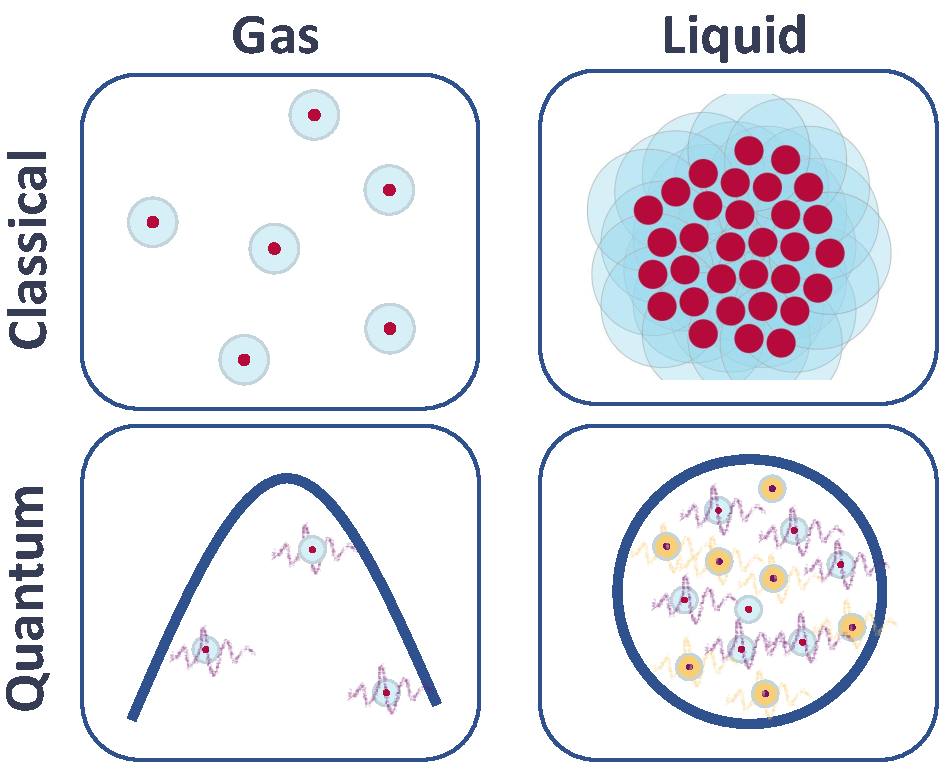
\includegraphics [width = 0.8 \linewidth]{Classical_and_quantum_droplet.pdf}
\end{center}
\caption[Comparison between classical and quantum liquid droplet]{Classical and quantum Liquid-gas phase transition. The upper panel shows a classical liquid-gas phase transition, explained by the famous Van der Waals equation. With this theory, particles interact with short-range hardcore (red solid part) and long-range attraction (light-blue outer). When the temperature lowers to the critical temperature, the sample undergoes a phase transition to be a liquid. As shown in the upper-right block, particles stay close to each other with inter-particle distance around the size of its hardcore. Meanwhile, their long-range parts overlap, showing a strongly correlated feature. For the lower panel, we draw the quantum liquid-gas phase transition for a BEC mixture sample. The thick blue line represents the shared wave function for the condensate part. The particle with a de-Broglie wave-packet represents the quantum depletion due to interaction excitation from the condensate. The right-bottom one shows the BEC mixture liquid droplet, which is the main topic of this thesis.}
\label{Classical_and_quantum_droplet}
\end{figure}

% to quantum matter, quantum gas sample (done: 2021年8月16日21:54:08)
Then, a question arises naturally for cold atom physicists: what about a quantum system? Is there any liquid phase for a Bose-Einstein condensate? A positive answer is made by Petrov in 2015 \cite{petrov2015}. For a dilute ultracold BEC mixture, we do have a liquid phase. However, this kind of liquid is dramatically different from the classical one. First, it is a zero-temperature sample, which means the thermal fluctuation is suppressed. Second, the sample is still dilute with an interparticle distance larger than 100 nm (interacting range typical around several nm). This indicates the system should be still in a weak-interacting case. Finally, quantum fluctuation shows its essential role. However, instead of serving as a driven force for mobility, the quantum fluctuation cures the sample's collapse or implosion. To study this sample, we could understand more profound the beyond mean-field correction of this many-body system.

% introduce quantum depletion and call droplet (done 2021年7月26日17:53:24)
As a new field in ultracold atoms, quantum liquid droplets originated from the deep understanding of the beyond mean-field theory of Bose-Einstein condensate (BEC) and from an innovative and careful extrapolation of textbook theory. In the past 25 years discovery of ultracold gases, mean-field theory (MF theory), as the zero-order solution of a many-body system, dominates the explanation of most phenomena. Especially for Bose-Einstein condensate, it explains plenty of interesting experiment observations, including the state of the equation for in-trap sample, excitation mode, dark soliton, bright solution, BEC collapse and so on. This zero-order approximation considers the condensates as a single wave-function \(\Psi\), which is based on the observation that most atoms share the same ground state, i.e. the \(k=0\) state (for uniform case). However, particles from the condensate could be excited to a finite momentum state due to the interaction between particles. From the microscopic theory of condensate, these particles with \(k>0\) have a fraction of order of \(\sqrt{na^3}\) compared to the condensate part, which occupies a tiny portion when the interaction is weak. Thus, we call it quantum depletion. This tiny portion brings only a tiny correction to its ground-state energy; so, people typical ignore its effect in most cases. However, things get incredibly different in the quantum liquid droplet; here, quantum depletion plays a vital role because the depletion part contributes a competitive energy scale to the mean-field energy. 

% what is quantum droplet? (done 2021年7月26日21:44:05)
Proposed by Petrov in 2015 \cite{petrov2015}, a BEC mixture with overall negative mean-field energy could survive from collapsing and form a quantum droplet. Surprisingly, this theory was first used to explain the self-bound behaviour in the dipolar gas \cite{ferrier2016Liquid,chomaz2016}. Then in 2018, Leticia group \cite{cabrera2018quantum} discovered the first double BEC droplet in a spin mixture of \(^{39}\)K. These two distinctive systems are related to the same theoretical explanation, showing the ubiquity that how important role for the LHY correction in ultracold atoms. For both cases, the mean-field energy approaches zero and is tuned by a Feshbach resonance for an inter-species \(s\)-wave contact interaction. Meanwhile, the LHY correction remains a positive value and grows even fast than the mean-field one when the density of the sample increasing. So, it cures the mean-field collapse. The difference between a dipolar droplet and a mixture BEC droplet is the inter-particle interaction type: for dipolar case, the interaction is anisotropic, which renders an anisotropic sample as well; however, for the BEC mixture case, thanks to the isotropic interaction, the sample shows a perfect spherical shape.

% droplet in different system (done: 2021年8月15日11:40:20)
As mentioned before, Petrov's theory was first used to the dipolar droplet \cite{ferrier2016Liquid,chomaz2016}, which is made of magnetic atoms with anisotropic interaction. Then in 2018, two groups \cite{cabrera2018quantum,semeghini2018self} produced the double BEC droplet exactly matching Petrov's original proposal. Latter, many works sprung up, in both experiment and theory. Leticia's group produce the droplet in a wave-guide \cite{cheiney2018bright}, in which they study the bright soliton to the droplet phase transition. From the low-dimension point of view, many theoretical proposals are developing, including \cite{petrov2016ultradilute,Ilg2018,Cui2021}. In another point of view, i.e. the gas phase sample with near-zero mean-field energy, theory \cite{Jorgensen2018}, and experiment \cite{skov2020} study the changing of monopole mode of an LHY gas. 

% why we study droplet? (done: 2021年8月15日19:44:00)
The initial purpose of our research was to make a heteronuclear droplet. With a rough calculation, we estimate its lifetime could reach about 100 ms, enabling us to do further research such as its excitation spectrum and the self evaporation. However, later we find the lifetime of the sample limited to 10 ms level. We attribute this to the large three-body loss between two species. Then, we have to turn our research goal to study the LHY effects in a double BEC of $^{23}$Na and $^{87}$Rb atoms in two different ways. First, we build the heteronuclear quantum liquid droplet in free space with more than $10^4$ atoms when the interspecies Na-Rb scattering length is tuned into the mean-field collapse regime. Under optimized conditions, a low-number-density droplet with a lifetime exceeding the observation time is observed. We also investigate the liquid-to-gas phase transition and obtain the critical atom numbers at the phase boundary. Second, we measure the release energies of two types of gas-phase mixtures, the pure in-trap gas and the gas formed after a droplet crosses the liquid-to-gas transition, and observe their opposite dependence on the interaction strength.  With calculations based on extended Gross-Pitaevskii equations (eGPEs), our results confirm the crucial contribution of $E_{\rm LHY}$ and its effects in stabilizing the heteronuclear double BEC far into the mean-field collapse region.

\section{Quantum depletion and LHY correction}
\label{sec:intro-LHY}

% Why discuss quantum depletion here (done 2021年8月17日13:20:01)
Back to the motivation of studying quantum droplets, the essential ingredient is the beyond-mend-field effect in a Bose condensate,i.e. the Lee-Huang-Yang (LHY) correction. LHY correction was first introduced by Lee, Huang and Yang in 1957~\cite{lee1957}, as the first-order correction of the ground state of Bose-Einstein condensate. However, due to its mighty contribution, we typically can ignore it. However, when the zero-order mean-field energy is approaching zero, which means the LHY correction could compare to the MF energy or even dominant the sample, we need to treat it more seriously. This section introduces the quantum depletion and LHY correction as a precursor for the next chapter, which discusses the complete theory for the quantum droplet.

% quantum depletion and LHY correction (done 2021年8月17日13:24:47)
Let us consider a Bose-Einstein condensate, with its Hamiltonian as
\begin{equation}
H=\sum_k\epsilon_k\hat{a}_k^\dagger\hat{a}_k+\frac{g}{2V}\sum_{\left\{k_i\right\}}\hat{a}_{k_1}^\dagger\hat{a}_{k_2}^\dagger\hat{a}_{k_3}\hat{a}_{k_4}
\end{equation}
By separating the condensate part and quantum fluctuation part, i.e. considering $a_0$ as $\sqrt{N}$ and write it away from other creation operators (with $k>0$), we have
\begin{equation}
\begin{split}
H=\frac{g N^2}{2V}&+\sum_{k\neq0}\left(\epsilon_k+gn_0\right)\hat{a}_k\dagger\hat{a}_k+\frac{gN}{2V}\sum_{k\neq0}\left(\hat{a}_k^\dagger\hat{a}_{-k}^\dagger+\hat{a}_k\hat{a}_{-k}\right)\\
&+\frac{g\sqrt{N}}{2V}\sum_{k_1+k_2+k_3=0}\left(\hat{a}_{k_1}^\dagger\hat{a}_{k_2}^\dagger\hat{a}_{k_3}+\hat{a}_{k_1}^\dagger\hat{a}_{k_2}\hat{a}_{k_3}\right)+\frac{g}{2V}\sum_{k_i\neq0}\hat{a}_{k_1}^\dagger\hat{a}_{k_2}^\dagger\hat{a}_{k_3}\hat{a}_{k_4}
\end{split}
\end{equation}
Ignore the higher order parts and do the Bogoliubov transition, we can get the diagonalized Hamiltonian as
\begin{equation}
\begin{split}
H\simeq \frac{g N^2}{2V}-\frac{1}{2}\sum _{k\neq 0} \left(\epsilon _k+\frac{g N}{V}-E_k\right)+\sum _{k\neq 0} E_k\hat{\alpha }_k^\dagger\hat{\alpha}_k\\
E_k=\sqrt{\epsilon_k\left(\epsilon_k+\frac{2gN}{V}\right)}=\sqrt{\frac{\hbar^2k^2}{2m}\left(\frac{\hbar^2k^2}{2m}+\frac{2gN}{V}\right)}
\end{split}
\end{equation}
The first part shows the energy shift (MF shift) for the condensate part. Second part shows summation of the energy of all particles with $k>0$, i.e. the quantum depletion. Third part shows the excitation spectrum of the sample and $E_k$ offers the dispersion of the sample. Now, we only consider the ground state properties, i.e. only consider the first two terms of the Hamiltonian. The fraction of depleted particle is
\begin{equation}
\frac{n_{\text{dp}}}{n}=\frac{8}{3\sqrt{\pi }}\sqrt{n a_S^3}
\end{equation}
where, we can directly read that with increasing of $n a_S^3$, more particles get out of the condensate. Meanwhile, these particles will contribute the LHY correction to ground state energy, i.e.
\begin{equation}
\frac{E_{\text{GS}}^R}{V}=\frac{g n^2}{2}\left(1+\frac{128}{15\pi ^{1/2}} \left(n a^3\right)^{1/2}\right)
\end{equation}
where $a=\left|a_S\right|$. We can find the LHY correction is small when density is low and only get important when $n a^3\sim 1$. These correction has been experimentally verified in strongly interacting Bose System \cite{Navon2011}. Thus, we find that this correction beyond mean-field theory increases the energy and increases ``hot'' particles. Moreover, considering the excitation spectrum for $g<0$, we can explain that the high energy excitation (short-wave) cure the unstable system of long-wave-instability, which gives the formation of LHY droplet \cite{petrov2015}.

% Historical study of LHY correction 放在第二章或者第五章

\section{Thesis Outline}
\label{sec:intro-outline}
% Outlines tells contents of each chapter (done: 2021年8月16日20:35:16)
Chapter \ref{Chap:theory} will discuss two fundamental conceptions: quantum scattering and the microscopic theory of a mixture of Bose condensate, which we will revisit many times in the following chapters. Chapter \ref{Chap_Apparatus} will introduce the main upgrades of apparatus for the droplet experiment. Chapter \ref{Chap_Feshbach} aims at achieving a precision mapping between scattering length and magnetic field, which is realized by a binding energy measurement of Feshbach molecules. After being armed with this accurate information of interaction, we detailed demonstrate the production of a hetero-nuclear droplet in Chapter \ref{Chap_droplet}. 
%In Chapter \ref{chap_LowD}, we turn to discuss droplets in low dimensions and try to offer a possibility of studying this fancy effect in the experiment. 
Finally, we summarize the thesis with some outlooks for future directions.

\chapterend

\chapter{Theory}
\label{Chap:theory}

% epigraph
\setlength{\unitlength}{1pt}
\setlength{\epigraphwidth}{10cm}
\epigraph{Law of physicists II: \\ Without theorists, experimentalists tend to falter. \cite{Lee:1992ui}}{--- T. D. Lee\\ \textit{History of the weak interactions (1987)}}

% goal of this chapter and structure of this chapter (done 2021-8-25 17:17:16)
This chapter discusses two fundamental things: quantum scattering theory and the theory of the quantum droplet. The quantum scattering theory is the basis for understanding the couple channel calculation in Chap. \ref{Chap_Feshbach}, which is used to fitting the binding energy of the Feshbach molecule to calibrate Na-Rb molecular potential. We note here that the scattering properties play an essential role in understanding the behaviour of an ultracold sample. The second part describes the microscopic theory for two-species BEC and analytically derives its LHY correction. Then, we demonstrate the theory of droplets made of the dual-species BEC. Latter in the Chap. \ref{Chap_droplet}, we implement both variational calculation and GPELab simulation for comparing to the experiment.

\section{Quantum scattering: Theory}
\label{sec:quan_scat}

We starting from the most general case, writing down a Bose system's Hamiltonian. Considering N spinless Bosons with mass m = 1 in volume V in 3-D space, and with thermal dynamic limit, i.e. N$\to \infty $ and V$\to
\infty $, and $\frac{N}{V}=n\to \text{finite}$), we write down the Hamiltonian
\begin{equation}
\begin{split}
\hat{H}_0&=\frac{1}{2}\int\nabla\hat{\Psi}^\dagger(x)\nabla\hat{\Psi }(x)dx=\frac{V}{(2\pi)^3}\int\epsilon_p^0\hat{a}_p^\dagger\hat{a}_pdp\\
\hat{H}_1&=\frac{1}{2}\int\hat{\Psi}^\dagger(x)\hat{\Psi}^\dagger(x')V(x-x')\hat{\Psi}(x')\hat{\Psi}(x)dxdx'=\frac{1}{2}\frac{V}{(2\pi)^3}\int V(p)\hat{a}_p^\dagger\hat{a}_{p'}^\dagger\hat{a}_{p'-q}\hat{a}_{p+q}dp
\end{split}
\end{equation}
with $\epsilon _p^0=\left.p^2\right/2$
For convenience we set $\hbar $ = 1.
where Fourier transformation for ladder operators are
\begin{equation}
\begin{split}
\hat{\Psi}(x)=\frac{1}{\sqrt{V}}\sum_{p}e^{ipx}\hat{a}_p=\frac{\sqrt{V}}{(2\pi)^3}\int dp e^{i p x}\hat{a}_p\\
\hat{\Psi}^\dagger(x)=\frac{1}{\sqrt{V}}\sum_p e^{-i p x}\hat{a}_p^\dagger=\frac{\sqrt{V}}{(2\pi)^3}\int dp e^{-i p x}\hat{a}_p^\dagger
\end{split}
\end{equation}
The interaction term $V(x-x')$ plays core role. Theoretically, it is hard to solve this problem because the real potential of atom-atom interaction is quite complicated. However, if we consider a special case, such that a bunch of Bose gas is quite dilute, we can use low-energy effective theory to tackle it.

There are three keywords for this special system: short-range interaction, dilute and low-temperature. 
Short-range gives a length scale $r_0$, which represent the inter-particle potential range. 
Dilute means: $n^{1/3}r_0<<1$, where n denote particle number density. 
Low temperature(energy) means $k r_0<<1$, where $k$ denotes momentum.

These three conditions allow us to ignore the complicated real potential between atoms, instead we can use scattering length (we will talk it later) to represent the whole scattering property of this system, especially at very low temperature left only one parameter, the s-wave scattering length $a_S$.

This note's material is arranged as following: first, we briefly talk about the basic scattering problem, which define $a_S$ in low temperature.
Then, we use mean field method solve Bose system, and discuss its ground state and excitation spectrum. Finally, we will go a little bit beyond the mean field theory, talking about quantum depletion and LHY correction.

\subsection{Scattering property}
The stationary Schrodinger equation and the Hamiltonian of the system is
\begin{equation}
\left(-\frac{\hbar ^2}{2m}\nabla ^2+\hat{V}(r)\right)\psi _k(r,\theta ,\phi )=\psi _k(r,\theta ,\phi )
\end{equation}
separating the state into radial and angular parts
\begin{equation}
\psi _k(r,\theta ,\phi )=R_l(k.r)Y_{\text{lm}}(\theta,\phi)
\end{equation}
and then the radial part equation
\begin{equation}
\left(\frac{d^2}{dr^2}+\frac{2}{r}\frac{d}{dr}-\frac{l(l+1)}{r^2}-\frac{2m}{\hbar ^2}V(r)+k^2\right)R_l(k,r)=0
\end{equation}
Then, we already know that the form of wave function when r is very large, i.e.
\begin{equation}
\psi (r)=e^{i k z}+f(k,\theta )\frac{e^{i k r}}{r}
\end{equation}
by spherical expanding we get:
For left side:
\begin{equation}
\psi (r)=\sum _{l =0}^{\infty } R_l(k,r)P_l(\text{Cos}[\theta ])
\end{equation}
For right side:
\begin{equation}
e^{i k z}=\sum _{l=0}^{\infty}(2l+1)i^l(kr)^{-1}\text{Sin}\left[k r-\frac{l \pi }{2}\right]P_l(\text{Cos}[\theta])
\end{equation}
\begin{equation}
f(k,\theta )=\sum _{l =0}^{\infty } f_l(k)P_l(\text{Cos}[\theta ])
\end{equation}
Thus we have the Radial part with different $l$ as
\begin{equation}
R_l(k,r)=(2l+1)i^l(k r)^{-1}\text{Sin}\left[k r-\frac{l \pi }{2}\right]+f_l(k)\frac{e^{i k r}}{r}
\end{equation}
Until now, we can only say that we find the connect between $R_l$ and $f_l$, however it doesn't help. But if we are treating some \pmb{finite range potential}, there exists a general solution:
Suppose that the potential can be written as
\begin{equation}
V(r)=\left\{
\begin{array}{c}
 V(r), r<r_0 \\
 0, r>r_0 \\
\end{array}
\right.
\end{equation}
When $r>r_0$ we have
\begin{equation}
\left(\frac{d^2}{dr^2}+\frac{2}{r}\frac{d}{dr}-\frac{l(l+1)}{r^2}+k^2\right)R_l(k,r)=0
\end{equation}
Solution of this equation has been solved well as following
\begin{equation}
R_l(k,r)=B_l(k)\text{SphericalBesselJ}[l,kr]+C_l(k)\text{SphericalBesselY}[l,\text{kr}]
\end{equation}
When r $\to \infty $, we get the asymptotic from of Bessel function as
\begin{equation}
R_l(k,r)=\frac{1}{k r}\left\{A_l(k)\text{Sin}\left[k r-\frac{l \pi }{2}-\delta _l(k)\right]\right\}
\end{equation}
where
\begin{equation}
A_l(k)=\sqrt{B_l^2(k)+C_l^2(k)},\text{  }\delta _l(k)=\text{ArcTan}\left[\frac{C_l(k)}{B_l(k)}\right]
\end{equation}
Comparing [12] and [16], we get that
\begin{equation}
f_l(k)=\frac{2l+1}{2i k}\left[e^{2i \delta _l(k)}-1\right]
\end{equation}
\begin{equation}
A_l(k)=(2l+1)i^le^{i \delta _l(k)}
\end{equation}
Finally, we have
\begin{equation}
f(k,\theta )=\sum _{l =0}^{\infty } \frac{2l+1}{2i k}\left[e^{2i \delta _l(k)}-1\right]P_l(\text{Cos}[\theta ])
\end{equation}
Now, if we connect the boundary condition inside $r_0$, we can totally solve out the $\delta _l(k)$ then solve out this problem.
For now, we can say that if we get all $\delta _l(k)$, then we solve this problems well. But that is a huge project because there are infinite $l$ and for each $l$, $\delta$ is a function of k, thus we need a good approximation for our system. Then, the last feature, low temperature, can be used. 
%\caption{Figure 1. For higher angular momentum $l$, it's hard to scatter with the short range hard core.}
As shown in figure, particles can hit this finite potential with $l$ less than 
\begin{equation}
l<l_{\max }=\frac{m v r_0}{\hbar }=r_0 k
\end{equation}
where $r_0$ is the potential range. Thus, At low-energy limit, i.e. $r_0k\to 0$, we have $l_{\max }\to 0$, which means we can consider S-wave only.
\begin{equation}
f_0(k)=\frac{1}{2ik}\left[e^{2i\delta_l(k)}-1\right]=\frac{1}{k}e^{i \delta _0(k)}\text{Sin}\left[\delta _0(k)\right]
\end{equation}
Thus, only one parameter $\delta _0(k)$ representing whole process. As historical preference, we introduce an equivalent parameter, scattering length $a_S$
\begin{equation}
a_s=a_0(k)|_{k\to0}=\underset{k\to0}{\text{Lim}}\left[-\frac{1}{k}\text{Tan}\left[\delta _0(k)\right]\right]
\end{equation}
where $a_s$ is independent with $k$, just as what we want.
Conclusion: when we deal with finite range potential scattering, not need to be finite intensity potential, and if the particle's momentum k is so small that $k<<\text{1/a}$, where a is the potential range, we can use only one parameter $a_0$ to describe the whole scattering process. The approximations made here are listed below:
Finite range potential gives $r_0$.
$k\ll 1\left/r_0 \right.$ where k is scattering momentum divided by $\hbar$, and $r_0$ is potential range
Scattering length $a_0$ actually depends on k, however if we consider the limit $k\to 0$, we can ignore this variance.
This very beautiful property gives us a way to deal with not-weak atom-atom scattering problem even with strong interaction.

\subsection{Resonance scattering}


\section{Quantum droplet: Theory}
% 
\subsection{Mean-field theory of Double BEC}
Now, we turn to describe double BEC with mean field theory, which will be used in Bose mixture droplet in journal club.

Hamiltonian for BEC with two species is
\begin{equation}
H_{\text{tot}}=\sum_k\epsilon_{1,k}\hat{a}_{1,k}\dagger\hat{a}_{1,k}+\frac{g_{11}}{2V}\sum_{\left\{k_i\right\}}\hat{a}_{1,k_1}^+\hat{a}_{1,k_2}^+\hat{a}_{1,k_3}\hat{a}_{1,k_4}+\sum_k\epsilon_{2,k}\hat{a}_{2,k}\dagger\hat{a}_{2,k}+\frac{g_{22}}{2V}\sum_{\left\{k_i\right\}}\hat{a}_{2,k_1}^+\hat{a}_{2,k_2}^+\hat{a}_{2,k_3}\hat{a}_{2,k_4}+\frac{g_{12}}{V}\sum_{\left\{k_i\right\}}\hat{a}_{2,k_1}^+\hat{a}_{1,k_2}^+\hat{a}_{1,k_3}\hat{a}_{2,k_4}
\end{equation}
where $k_1+k_2=k_3+k_4$, satisfy momentum conservation.$g_{\text{ii}}$ represent intra-interaction strength, and $g_{12}$ for inter-interaction.
$\hat{a}_{i,k}^+$($\hat{a}_{i,k}$) denote the ladder operator for $i^{\text{th}}$ component.
Because of the special role of the state with k = 0, i.e. condensate, we separate ladder operator into two piece for whole Bose gas
\begin{equation}
\hat{\Psi }_i(x)=\frac{1}{\sqrt{V}}\sum_{p\neq0}e^{ipx}\hat{a}_{i,p}+\frac{1}{\sqrt{V}}\hat{a}_{i,0}=\hat{\Psi }_i'(x)+\frac{1}{\sqrt{V}}\hat{a}_{i,0}
\end{equation}
\begin{equation}
\hat{\Psi }_i\dagger(x)=\frac{1}{\sqrt{V}}\sum_{p\neq0}e^{-ipx}\hat{a}_{i,p}\dagger+\frac{1}{\sqrt{V}}\hat{a}_{i,0}\dagger=\hat{\Psi}'\dagger(x)+\frac{1}{\sqrt{V}}\hat{a}_{i,0}\dagger
\end{equation}
Then we get Hamiltonian as
\begin{equation}
\begin{split}
H=\frac{g_{11}N_1^2+g_{22}N_2^2+2g_{12}N_1N_2}{2V}+\sum _{k\neq 0} \left(\epsilon _{1,k}+\frac{g_{11}N_1+g_{12}N_2}{V}\right)\hat{a}_{1,k}\dagger\hat{a}_{1,k}+\sum_{k\neq 0} \left(\epsilon _{2,k}+\frac{g_{22} N_2+g_{12}N_1}{V}\right)\hat{a}_{2,k}\dagger\hat{a}_{2,k}+\\
\frac{g_{11} N_1}{2V}\sum _{k\neq 0} \left(\hat{a}_{1,k}^+\hat{a}_{1,-k}^++\hat{a}_{1,k}\hat{a}_{1,-k}\right)+\frac{g_{22} N_2}{2V}\sum_{k\neq0}\left(\hat{a}_{2,k}^+\hat{a}_{2,-k}^++\hat{a}_{2,k}\hat{a}_{2,-k}\right)+\frac{g_{12}\sqrt{N_1N_2}}{2V}\sum _{k\neq 0} \left(\hat{a}_{1,k}^+\hat{a}_{2,k}+\hat{a}_{2,k}^+\hat{a}_{1,k}+\hat{a}_{1,k}\hat{a}_{2,-k}+\hat{a}_{2,k}^+\hat{a}_{1,-k}^+\right)
\end{split}
\end{equation}
where we only keep the second order of $N_i$, dropping third and forth order of $N_i$. Then, diagonalize this Hamiltonian by extended Bogoliubov transformation for double BEC, we have
\begin{equation}
H=\frac{g_{11}N_1^2+g_{22}N_2^2+2g_{12}N_1N_2}{2V}+\frac{1}{2}\sum _{k\neq 0} \left(E_++E_--\frac{\hbar ^2k^2}{2m_1}-\frac{\hbar ^2k^2}{2m_2}-\frac{g_{11}N_1+g_{22}N_2}{V}\right)+\sum_{k\neq 0} E_{+,k}\hat{a}_{+,k}\dagger\hat{a}_{+,k}+\sum _{k\neq 0} E_{-,k}\hat{a}_{-,k}\dagger\hat{a}_{-,k}
\end{equation}
where
\begin{equation}
E_{\pm }=\sqrt{\frac{\omega _1^2+\omega _2^2}{2}\pm \sqrt{\left(\frac{\omega _1^2-\omega _2^2}{2}\right){}^2+\frac{g_{12}^2N_1N_2}{V^2}\frac{\hbar
^2k^4}{m_1m_2}}}
\end{equation}
where
\begin{equation}
\omega _i=\sqrt{\frac{\hbar ^2k^2}{2m_i}\left(\frac{\hbar ^2k^2}{2m_i}+\frac{2g_{\text{ii}}N_i}{V}\right)}
\end{equation}
We plot the spectrum for each channel $E_+$ and $E_-$, with $\text{$\delta $g}=\sqrt{g_{11}g_{22}}-g_{12}>0$ and $\text{$\delta $g}=\sqrt{g_{11}g_{22}}-g_{12}<0$
Where we find similar spectrum with one component BEC. For $\text{$\delta $g}<0$, we get complex energy with small $k$, which represent unstable of the system.

\subsection{Ground state energy and LHY correction}
Ground state energy will be
\begin{equation}
E_{\text{GS}}=\frac{g_{11}N_1^2+g_{22}N_2^2+2g_{12}N_1N_2}{2V}+\frac{1}{2}\sum _{k\neq0}\left(E_++E_--\frac{\hbar^2k^2}{2m_1}-\frac{\hbar ^2k^2}{2m_2}-\frac{g_{11}N_1+g_{22}N_2}{V}\right)
\end{equation}
After re-normalization we have
\begin{equation}
E_{\text{GS}}^R=\frac{g_{11}N_1^2+g_{22}N_2^2+2g_{12}N_1N_2}{2V}+\frac{1}{2}\sum _{k\neq 0} \left(E_++E_--\frac{\hbar ^2k^2}{2m_1}-\frac{\hbar^2k^2}{2m_2}-\frac{g_{11}N_1+g_{22}N_2}{V}+\frac{m_1g_{11}^2N_1^2/V^2+m_2g_{22}^2N_2^2/V^2+4\frac{m_1m_2}{m_1+ m_2}g_{12}^2N_1N_2/V^2}{\hbar ^2k^2}\right)
\end{equation}
The second term is LHY term which can be rewritten as
\begin{equation}
E_{\text{LHY}}=\frac{1}{2}\sum _{k\neq0}\left(\sqrt{\frac{\omega _1^2+\omega _2^2}{2}+\sqrt{\left(\frac{\omega_1^2-\omega_2^2}{2}\right){}^2+g_{12}^2n_1n_2\frac{\hbar^4k^4}{m_1m_2}}}+\sqrt{\frac{\omega _1^2+\omega_2^2}{2}-\sqrt{\left(\frac{\omega_1^2-\omega _2^2}{2}\right){}^2+g_{12}^2n_1n_2\frac{\hbar^4k^4}{m_1m_2}}}-\frac{\hbar^2k^2}{2m_1}-\frac{\hbar^2k^2}{2m_2}-g_{11}n_1-g_{22}n_2+\frac{m_1g_{11}^2n_1^2+m_2g_{22}^2n_2^2+4\frac{m_1m_2}{m_1+m_2}g_{12}^2n_1n_2}{\hbar ^2k^2}\right)
\end{equation}
into integral formation
\begin{equation}
\frac{E_{\text{LHY}}}{V}=\int _0^{k_c}\frac{k^2}{4\pi ^2}\left(\sqrt{\frac{\omega_1^2+\omega_2^2}{2}+\sqrt{\left(\frac{\omega_1^2-\omega_2^2}{2}\right){}^2+g_{12}^2n_1n_2\frac{\hbar^4k^4}{m_1m_2}}}+\sqrt{\frac{\omega_1^2+\omega_2^2}{2}-\sqrt{\left(\frac{\omega_1^2-\omega_2^2}{2}\right){}^2+g_{12}^2n_1n_2\frac{\hbar^4k^4}{m_1m_2}}}-\frac{\hbar^2k^2}{2m_1}-\frac{\hbar^2k^2}{2m_2}-g_{11}n_1-g_{22}n_2+\frac{m_1g_{11}^2n_1^2+m_2g_{22}^2n_2^2+4\frac{m_1m_2}{m_1+ m_2}g_{12}^2n_1n_2}{\hbar ^2k^2}\right)dk
\end{equation}
\begin{equation}
\begin{split}
\frac{E_{\text{LHY}}}{V}=C_1\int _0^{k_c}\frac{\tilde{k}^2}{4\pi ^2}\left(\sqrt{\frac{1}{2}\left(\frac{\tilde{k}^2}{2}\left(\frac{\tilde{k}^2}{2}+2\right)+\frac{1}{\gamma^2}\frac{\tilde{k}^2}{2}\left(\frac{\tilde{k}^2}{2}+2y\gamma\right)\right)+\sqrt{\left(\frac{1}{2}\left(\frac{\tilde{k}^2}{2}\left(\frac{\tilde{k}^2}{2}+2\right)-\frac{1}{\gamma^2}\frac{\tilde{k}^2}{2}\left(\frac{\tilde{k}^2}{2}+2y \gamma \right)\right)\right)^2+\frac{xy}{\gamma }\tilde{k}^4}}+\right.\\
\left.\sqrt{\frac{1}{2}\left( \frac{\tilde{k}^2}{2}\left(\frac{\tilde{k}^2}{2}+2\right)+\frac{1}{\gamma ^2}\frac{\tilde{k}^2}{2}\left(\frac{\tilde{k}^2}{2}+2y\gamma \right)\right)-\sqrt{\left(\frac{1}{2}\left(\frac{\tilde{k}^2}{2}\left(\frac{\tilde{k}^2}{2}+2\right)-\frac{1}{\gamma ^2}\frac{\tilde{k}^2}{2}\left(\frac{\tilde{k}^2}{2}+2y\gamma \right)\right)\right)^2+\frac{xy}{\gamma}\tilde{k}^4}}-\frac{\tilde{k}^2}{2}\left(1+\frac{1}{\gamma }\right)-1-y+\frac{1+\gamma y^2+\frac{4xy \gamma}{1+\gamma}}{\tilde{k}^2}\right)d\tilde{k}
\end{split}
\end{equation}

\begin{equation}
\begin{split}
C_1=g_{11}n_1\left(\frac{\sqrt{m_1g_{11}n_1}}{\hbar }\right){}^3\\
\gamma =\frac{m_2}{m_1}\\
x=\frac{g_{12}^2}{g_{11}g_{22}}\\
y=\frac{g_{22}n_2}{g_{11}n_1}\\
\tilde{k}=\frac{\hbar  k}{\sqrt{m_1g_{11}n_1}}
\end{split}
\end{equation}
\begin{equation}
\frac{\omega _1}{g_{11}n_1}=\sqrt{\frac{\hbar^2k^2}{2m_1g_{11}n_1}\left(\frac{\hbar^2k^2}{2m_1g_{11}n_1}+2\right)}=\sqrt{\frac{\tilde{k}^2}{2}\left(\frac{\tilde{k}^2}{2}+2\right)}
\end{equation}
\begin{equation}
\frac{\omega _2}{g_{11}n_1}=\sqrt{\frac{\hbar^2k^2}{2m_2g_{11}n_1}\left(\frac{\hbar^2k^2}{2m_2g_{11}n_1}+2\frac{g_{22}n_2}{g_{11}n_1}\right)}=\sqrt{\frac{1}{\gamma}\frac{\tilde{k}^2}{2}\left(\frac{1}{\gamma}\frac{\tilde{k}^2}{2}+2y\right)}=\frac{1}{\gamma}\sqrt{\frac{\tilde{k}^2}{2}\left(\frac{\tilde{k}^2}{2}+2y\gamma \right)}
\end{equation}
we take out the dimensionless part of it, i.e.
\begin{equation}
E_{\text{GS}}^R=\frac{g_{11}N_1^2+g_{22}N_2^2+2g_{12}N_1N_2}{2V}+\frac{8V}{15\pi^2}m_1^{3/2}\left(g_{11}n_1\right){}^{5/2}f\left(\frac{m_2}{m_1},\frac{g_{12}^2}{g_{11}g_{22}},\frac{g_{22}n_2}{g_{11}n_1}\right)
\end{equation}
Where $f$ is always larger than 0 and is dimensionless.
We will show in this week's journal club that, the second term of LHY correction will actually stabilize the system from collapse and will not require entering strong interaction regime.

\begin{equation}
\frac{1}{2}\left(
\begin{array}{cc}
 n_1 & n_2 \\
\end{array}
\right)\left(
\begin{array}{cc}
 g_{11} & g_{12} \\
 g_{12} & g_{22} \\
\end{array}
\right)\left(
\begin{array}{c}
 n_1 \\
 n_2 \\
\end{array}
\right)
\end{equation}
diagonalize
\begin{equation}
\lambda _+=\frac{g_{11}+g_{22}}{2},\lambda_-=\frac{\sqrt{g_{11}g_{22}}}{g_{11}+g_{22}}\text{$\delta $g}
\end{equation}
\begin{equation}
n_+=\frac{n_1\sqrt{g_{11}}-n_2\sqrt{g_{22}}}{\sqrt{g_{11}+g_{22}}}, n_-=\frac{n_1\sqrt{g_{22}}+n_2\sqrt{g_{11}}}{\sqrt{g_{11}+g_{22}}}
\end{equation}






% from intro about the LHY correction and quantum depletion

\section{Temp: Dilute Bose system: Pseudo-Hamiltonian and Bogoliubov transformation}
As we can use $a_S$ representing scattering process, we can write down a pseudo-potential, which gives the same effect as the original one. This procedure first done by \textit{Fermi} as following
\begin{equation}
V(r)=g \delta (r)\partial _r\cdot r=\frac{4\pi\hbar^2a_S}{m}\delta (r)\partial _r\cdot r
\end{equation}
which is a contact potential only affect two atoms when they have same $r$. The last term $\partial _r\cdot r$ eliminates wave function's divergence at $r\to 0$, due to it has form of $\psi \to 1-\left.a_S\right/r$. if we write the potential as
\begin{equation}
V(r)=g_R\delta (r)
\end{equation}
where $g_R$ denotes the interaction intensity. Note that this $g_R$ cannot be considered as physics quantity due to its divergence at $r\to 0$. However, the relationship between $g_R$ and $g$ can be obtain by \textit{Dyson} Equation.
\begin{equation}
g_R=g+g \Sigma ^* g_R
\end{equation}
where $g_R$ represent normalized interaction strength, and $\Sigma$ represent the proper self-energy of system, i.e.
\begin{equation}
g_R=\frac{4\pi  \hbar ^2a_S}{m}\left(1+\frac{g_R}{V}\sum _{k=0}^{\infty } \frac{1}{\hbar ^2\left.k^2\right/m}\right)
\end{equation}
by just take the second order correction (loop correction), we get
\begin{equation}
g_R=g\left(1+\frac{g}{V}\sum _{k=0}^{\infty } \frac{1}{\hbar ^2\left.k^2\right/m}\right)
\end{equation}
The second term is actually diverge, which represents high energy scattering. This term will only be used when we need to sum over some term with all high energy collision process. In most time, we can just take $g$ as
\begin{equation}
g=\frac{4\pi  \hbar ^2a_S}{m}
\end{equation}
Then, we can rewrite the whole Hamiltonian as following
\begin{equation}
\begin{split}
\hat{H}_0&=\frac{1}{2}\int \nabla \hat{\Psi }\dagger(x)\nabla \hat{\Psi }(x)dx\\
H_1&\simeq \frac{1}{2}\int \hat{\Psi }\dagger(x)\hat{\Psi }\dagger(x')g \delta (x-x')\hat{\Psi }(x')\hat{\Psi }(x)dxdx'=\frac{g}{2}\int \hat{\Psi}\dagger(x)\hat{\Psi }\dagger(x)\hat{\Psi }(x)\hat{\Psi }(x)dx
\end{split}
\end{equation}
Fourier transformation gives the Hamiltonian in momentum space as
\begin{equation}
H_{\text{pseudo}}=\sum_k\epsilon_k\hat{a}_k\dagger\hat{a}_k+\frac{g}{2V}\sum _{\left\{k_i\right\}}\hat{a}_{k_1}^+\hat{a}_{k_2}^+\hat{a}_{k_3}\hat{a}_{k_4}
\end{equation}
where $k_1+k_2=k_3+k_4$, satisfies momentum conservation. This is just the pseudo-Hamiltonian for many-Boson system.
Because of the special role of the state with k = 0, i.e. condensate, we separate ladder operator into two piece for whole Bose gas
\begin{equation}
\hat{\Psi }(x)=\frac{1}{\sqrt{V}}\sum _{p\neq 0} e^{i p x}\hat{a}_p+\frac{1}{\sqrt{V}}\hat{a}_0=\hat{\Psi }'(x)+\frac{1}{\sqrt{V}}\hat{a}_0
\end{equation}
\begin{equation}
\hat{\Psi }\dagger(x)=\frac{1}{\sqrt{V}}\sum _{p\neq 0} e^{-i p x}\hat{a}_p\dagger+\frac{1}{\sqrt{V}}\hat{a}_0\dagger=\hat{\Psi }'\dagger(x)+\frac{1}{\sqrt{V}}\hat{a}_0\dagger
\end{equation}
where $\hat{a}_0=\hat{a}_0\dagger=\sqrt{n}=\sqrt{\frac{N}{V}}$
notice that {``}mean field{''} just means taking some quantum operator as a c-number, which is average of this operator, so the quantum fluctuation is blurred. So, when we use mean field theory to calculate the system ,we need pay attention to what fluctuation we take it from the calculation, then at necessary time, we can get it back.
put them into (31), then simply
\begin{equation}
\begin{split}
H=\frac{g N^2}{2V}&+\sum_{k\neq0}\left(\epsilon_k+gn_0\right)\hat{a}_k\dagger\hat{a}_k+\frac{gN}{2V}\sum_{k\neq0}\left(\hat{a}_k^+\hat{a}_{-k}^++\hat{a}_k\hat{a}_{-k}\right)\\
&+\frac{g\sqrt{N}}{2V}\sum_{k_1+k_2+k_3=0}\left(\hat{a}_{k_1}^+\hat{a}_{k_2}^+\hat{a}_{k_3}+\hat{a}_{k_1}^+\hat{a}_{k_2}\hat{a}_{k_3}\right)+\frac{g}{2V}\sum_{k_i\neq0}\hat{a}_{k_1}^+\hat{a}_{k_2}^+\hat{a}_{k_3}\hat{a}_{k_4}
\end{split}
\end{equation}
Here, we drop the terms with N's order less than $N$, because they became very smaller than formers when temperature is quite low that large amount of atoms are condensate. (If considering the last two term, we will get the Beliaev-Landau Damping.)
\begin{equation}
H_{\text{pseudo}}\simeq\frac{gN^2}{2V}+\sum_{k\neq0}\left(\epsilon _k+g n_0\right)\hat{a}_k\dagger\hat{a}_k+\frac{gn_0}{2}\sum_{k\neq0}\left(\hat{a}_k^+\hat{a}_{-k}^++\hat{a}_k\hat{a}_{-k}\right)\end{equation}
Now, as quadratic form, we can diagonalize it with so called Bogoliubov transformation
\begin{equation}
\begin{split}
\hat{a}_k=u_k\hat{\alpha }_k-v_k\alpha _{-k}^+\\
\hat{a}_{-k}=u_k\hat{\alpha }_{-k}-v_k\alpha _k^+
\end{split}
\end{equation}
where $\alpha _k^+\left(\alpha _k\right)$ is a new ladder operator, which actually denote create(annihilate) a quasi-particle in this condensate system. $u_k$ and $v_k$ is c-number as function of $k$ and $E_k$, which gives the spectrum of quasi-particle. 
Finally, we give out the diagonalized Hamiltonian as
\begin{equation}
\begin{split}
H_{\text{pseudo}}\simeq \frac{g N^2}{2V}-\frac{1}{2}\sum _{k\neq 0} \left(\epsilon _k+\frac{g N}{V}-E_k\right)+\sum _{k\neq 0} E_k\hat{\alpha }_k\dagger\hat{\alpha
}_k\\
E_k=\sqrt{\epsilon _k\left(\epsilon _k+\frac{2 g N}{V}\right)}=\sqrt{\frac{\hbar ^2k^2}{2m}\left(\frac{\hbar ^2k^2}{2m}+\frac{2 g N}{V}\right)}
\end{split}
\end{equation}
%Here needs a figure
%\caption{Figure 2. This plot shows the dissipation relation ship for quasi-particle in the Bose-condensation. When k is small, it looks like a phonon, however, when k goes large it back to a particle-like quasi-particle.}
Note that the gap-less linear low energy excited dissipation relation gives the super fluid property. when $k$ get larger, it turn back to classical particle.
Now, let's consider what happens when $g<0$, i.e. attractive potential between atoms. The excitation spectrum will be
%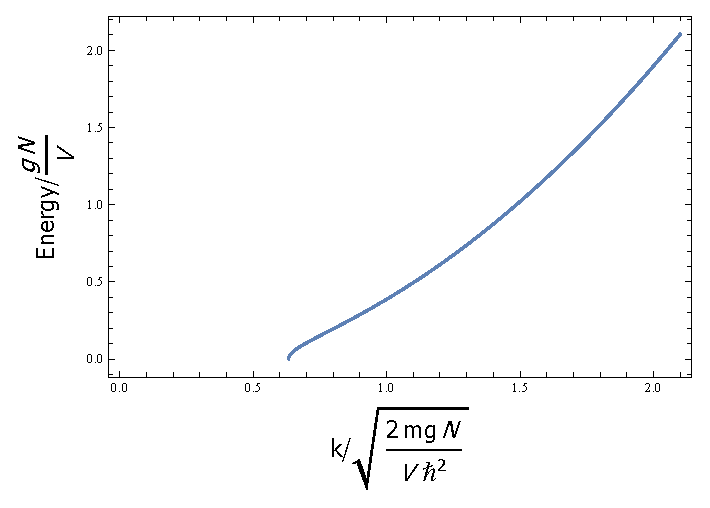
\includegraphics{Note for review_gr2.eps}
%\caption{Figure 3. This plot shows the dissipation relationship for attractive Bose-system.}
We find no excitation for small $k$, which means ground state has non-zero momentum, violating our assumption that condensate stay at $k=0$.
Thus, this result actually tells us that this attractive Bose-gas can not exist stable. We will return to this point later, when we talk about the ground state energy of this Bose system and also for double BEC case.

\subsection{Ground state and LHY correction}
Now we consider the ground state of this system. Directly take the lowest energy level from (38), we have
\begin{equation}
\begin{split}
E_{\text{GS}}=\frac{g N^2}{2V}-\frac{1}{2}\sum _{k\neq 0} \left(\epsilon _k+\frac{g N}{V}-E_k\right)
\end{split}
\end{equation}
where first term represent the mean field energy shift from {``}vacuum{''}, and second term come from quantum fluctuation (at zero temperature), i.e.
\begin{equation}
-\frac{1}{2}\sum _{k\neq 0} \left(\epsilon _k+\frac{g N}{V}-E_k\right)=-\frac{1}{2}\sum _{k\neq 0} \left(\frac{\hbar ^2k^2}{2m}+\frac{g N}{V}-\sqrt{\frac{\hbar
^2k^2}{2m}\left(\frac{\hbar ^2k^2}{2m}+\frac{2 g N}{V}\right)}\right)
\end{equation}
If you plot the term in the summation, you will find it decays with k increasing. However, if we expand it in series, we have 
\begin{equation}
\begin{split}
\frac{\hbar ^2k^2}{2m}&+\frac{g N}{V}-\sqrt{\frac{\hbar ^2k^2}{2m}\left(\frac{\hbar ^2k^2}{2m}+\frac{2 g N}{V}\right)}\\
&=\frac{1}{2}\left(\frac{gN}{V}\right)^2\left(\frac{2m}{\hbar^2}\right)\frac{1}{\pmb{k^2}}-\frac{1}{2}\left(\frac{gN}{V}\right)^3\left(\frac{2m}{\hbar^2}\right)^2\frac{1}{\pmb{k^4}}+\frac{5}{8}\left(\frac{gN}{V}\right)^4\left(\frac{2m}{\hbar^2}\right)^3\frac{1}{\pmb{k^6}}+\text{...}
\end{split}
\end{equation}
with leading proportional to $\frac{1}{k^2}$, we have divergence when sum over k to infinite. This divergence is due to the pseudo-potential with $\delta (r)$ actually does not allow calculation for large $k$, thus, we need do re-normalization to truncate this $\frac{1}{k^2}$ divergence.
Recalling the re normalized interaction $g_R$ in (27), we have
\begin{equation}
g_R=g+\frac{g^2}{V}\sum _k \frac{m}{\hbar ^2k^2}
\end{equation}
Then total energy will be
\begin{equation}
E_{\text{GS}}^R=\frac{gN^2}{2V}-\frac{1}{2}\sum_{k\neq0}\left(\frac{\hbar ^2k^2}{2m}+\frac{gN}{V}-\sqrt{\frac{\hbar^2k^2}{2m}\left(\frac{\hbar^2k^2}{2m}+\frac{2gN}{V}\right)}-\left(\frac{gN}{V}\right)^2\left(\frac{2m}{\hbar ^2}\right)\frac{1}{k^2}\right)
\end{equation}
Directly do this summation, we get the famous LHY correction
\begin{equation}
\frac{E_{\text{GS}}^R}{V}=\frac{g n^2}{2}\left(1+\frac{128}{15\pi ^{1/2}} \left(n a^3\right)^{1/2}\right)
\end{equation}
where $a=\text{Abs}\left[a_S\right]$. Now, we plot ground state energy when $g>0$
Where we can find the LHY correction is small when density is low, and only get important when $n a^3\sim 1$. These correction has been experimentally verified in strong interacting Bose System [PRL 107, 135301].
Then we plot the ground state energy with $g<0$
%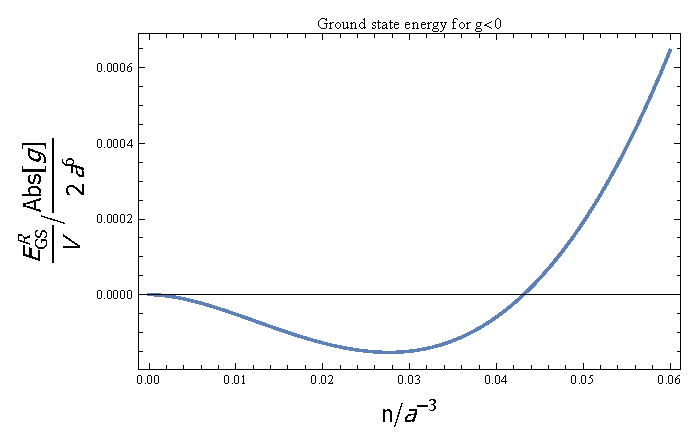
\includegraphics{Note for review_gr3.eps}
Where we find that only when \begin{equation}n a^3>0.028\end{equation}, the ground state energy increase with n increasing, which means stable ground state exist. This stability is reached due to quantum fluctuation resisting the collapse from attractive interacting, which has the same mechanics of liquid droplet in which stability is reached due to Van de Waals force. This so called LHY droplet seems haven{'}t been observed in experiment, I guess main reason is when $n a^3$ get large, the many body loss will be severe, which hides the phenomenon of droplet. We will talk more about the mechanics of LHY droplet when we considering the quantum depletion.

\subsection{Quantum Depletion and Mechanism of LHY Droplet}
Let's now consider: in a ground state of BEC at zero temperature, how many particles will not stay at $k=0$ state? The answer is just directly summation all non-zero k state in the ground state. as following
\begin{equation}
n_{\text{dp}}=\frac{1}{V}\sum _{k\neq 0} v_k^2=\frac{1}{3\pi ^2}\left(\frac{m c}{\hbar }\right)^3\propto \xi ^{-3}
\end{equation}
where $v_k$ is parameter in Bogoliubov transformation, $c =\sqrt{\frac{g n}{2m}}$ is the first sound speed in BEC, and $\xi =\frac{\hbar }{\sqrt{2m g n}}$ is healing length.
The fraction of depleted particle is
\begin{equation}
\frac{n_{\text{dp}}}{n}=\frac{8}{3\sqrt{\pi }}\sqrt{n a_S^3}
\end{equation}
we can directly read that with increasing of $n a_S^3$, more particles get out of the condensate. Meanwhile, these particles will contribute the LHY correction to ground state energy. Thus, we find that this correction beyond mean field theory actually always increase the energy and also increase {``}hot{''} particles. Moreover, if you consider the excitation spectrum for $g<0$, you can explain that the high energy excitation(short-wave)
actually cure the unstable system from long-wave-instability, which gives the formation of LHY droplet.

%For a single species condensate, with the mean-field approximation, we have its energy density propotional to \(n^2\). This is valid for low density case, which satisfies \(na_s^3<<1\). When the condition is brocken, we need a correction to further describe its behaviour, i.e. the LHY correction. From the view of ground state energy, this correction is with order of \(na_s^3\) comparing to the mean-field part, which in most case is too weak to detect. 
%这里从历史角度出发,谈历史上是如何测量LHY correction的

% discuss quantum depletion in this part
%From another point of view, i.e. how many particle stay beyond the zero momentum state, we need to introduce the quantum depletion. Similar to thermal depletion of a condensate, the quantum depletion is excited due to the inter-particle interaction. The depletion density can be written as




\chapterend


\chapter{Apparatus}
\label{Chap_Apparatus}

% epigraph (done 2021-8-24 09:23:49)
\setlength{\unitlength}{1pt}
\setlength{\epigraphwidth}{10.5cm}
\epigraph{工欲善其事,必先利其器。\\ A craftsman must sharpen his tools to do his job.}{--- Confucius\\ \textit{The Analects (5th century BC)}}

% introduction (done 2021-9-16 16:08:33)
This chapter describes the Na-Rb machine and the upgrades we made for our droplet experiment. As most of the setup has been described by the previous thesis \cite{WangFudong2016Soau,LiXiaoke2015Chsd}, we only shortly make a summary in Sec. \ref{sec:machine} for the completeness of this chapter. In Sec. \ref{sec:image}, we turn to the image system upgrades for measuring the droplet sample with several $\mu$m sizes. We design a 15$\times$ magnification image system with a resolution of 2 $\mu$m. Besides, we upgraded the mechanical part onto an electro-translation stage, which can follow the ToF of the free-falling sample without worsening the image resolution. We detailedly describe the high-magnetic field in-situ image scheme for subtracting the sample's density profile reliable. To control more cameras from different manufacturers, I built a multi-camera control platform with image processing called CAMIMA. We will introduce it in Sec. \ref{sec:camima} as a manual for future using and upgrading. Finally, we discuss several improvements such as fast-coil for fast controlling magnetic field (Sec. \ref{sec:fastcoil}), magnetic field gradient compensation (Sec. \ref{subsec:gradientcompen}) and coil antennas for increasing the Rabi frequency of Rb (Na) micro-wave transition (Sec. \ref{subsec:FWLA}).

\section{Overview: the Na-Rb machine I}
\label{sec:machine}

% goal of this Na-Rb machine (done 2021-8-24 10:28:43)
A cold atom machine capable of producing reproducible samples with stable atomic conditions is indispensable for the following experiments. So, even though the Na-Rb machine in our laboratory has been running for longer than eight years, many aspects still need to improve to make the sample condition more stable. \cite{LiLintao2021} describes many efforts we made: optimization of the micro-wave evaporation procedure for Rb sympathies cooling of Na; a new ultra-stable magnetic field servo system for achieving hundred-Gauss with only two mG level fluctuation. Besides stability, producing more atoms is another goal for many experiments because there are always various types of loss during preparing the atomic (or molecular) samples. More numbers of final sample can make detection easier and offer more opportunities to study new physics. In the droplet experiment \cite{guo2021leehuangyang}, if we produce a sample with ten times more numbers (i.e. $10^6$ for each species), we can study more properties of the bulk sample, such as flat-top density profile \cite{petrov2015}, the surface excitation modes \cite{petrov2015} and achieving a longer lifetime.

% overall system (done 2021-9-16 17:18:52)
\begin{figure}[htb]
\begin{center}
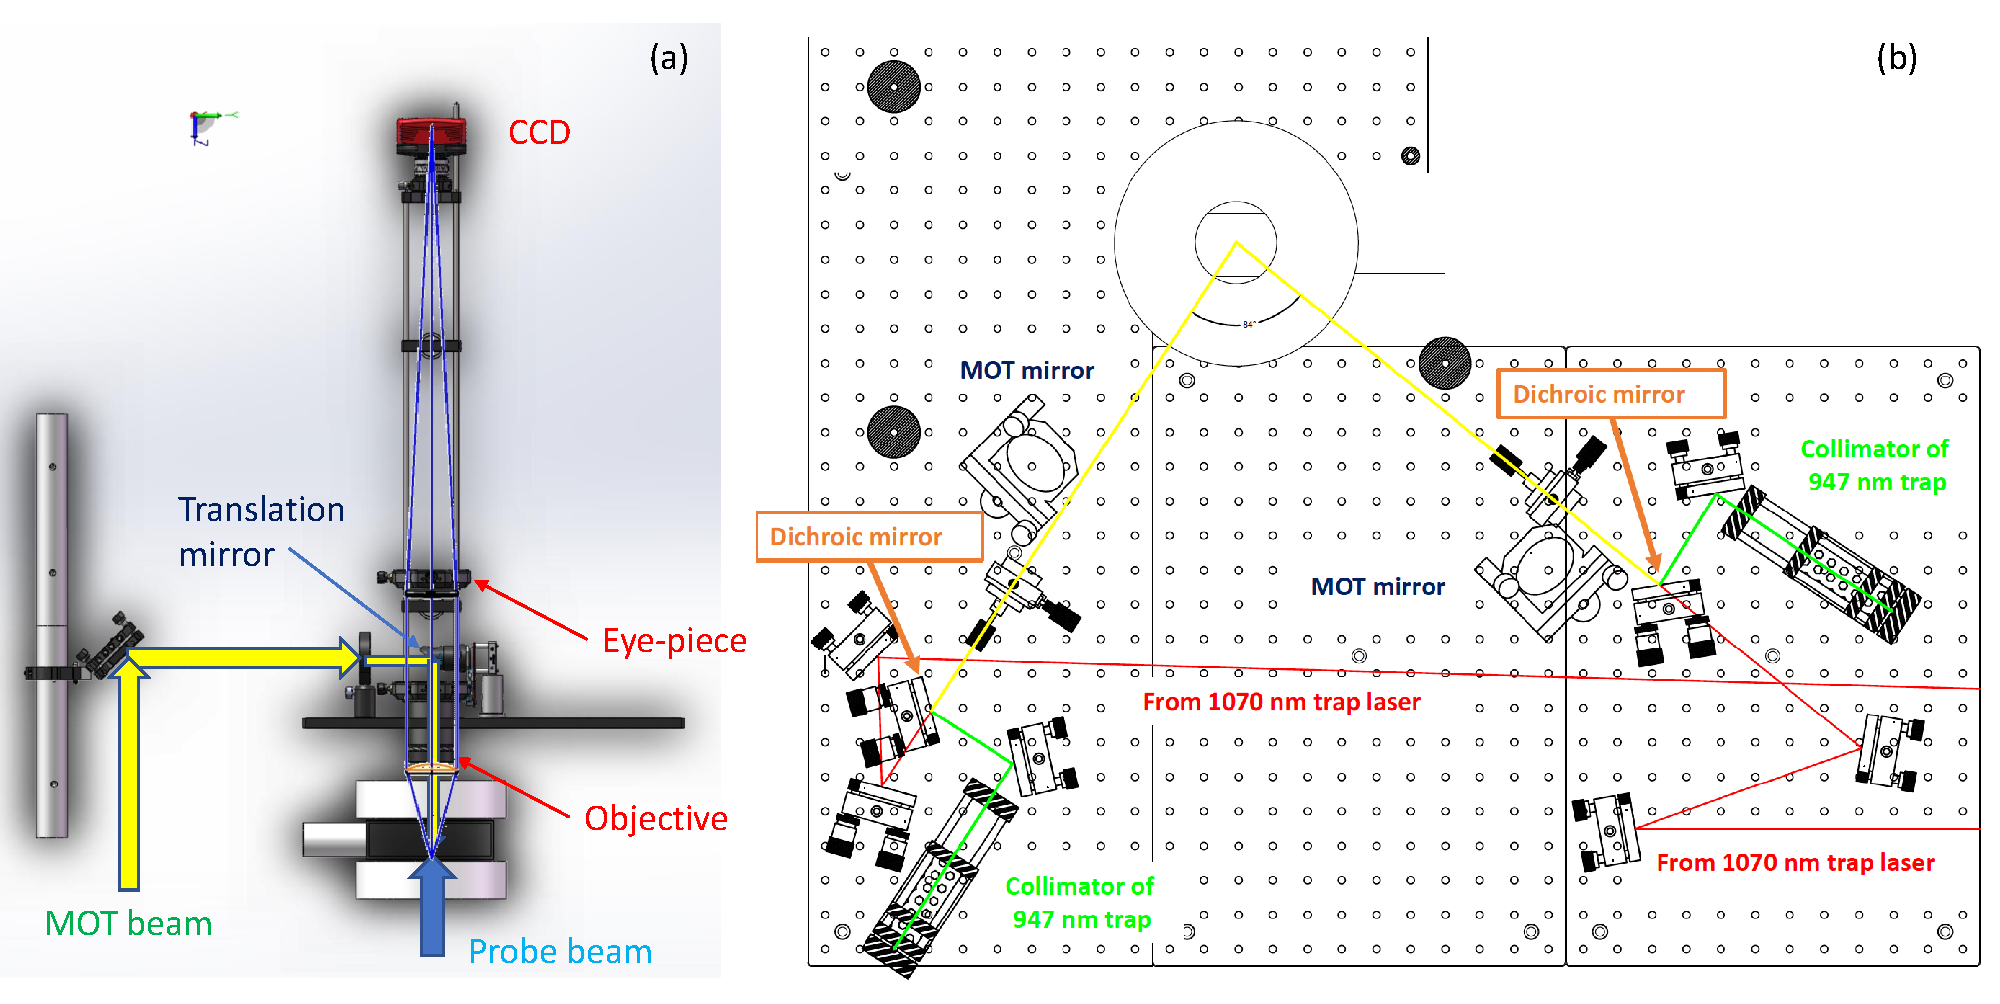
\includegraphics[width = \linewidth]{figures/Apparatus_overall.pdf}
\end{center}
\caption[Front and top view of overall Na-Rb machine]{(a) shows the Front view of the Na-Rb machine. The up-down image(pumping) shares the same optical path with MOT laser. After MOT loading, we switch the mirror cart away to leave path for up-down image. (b) shows the optical trap laser layout as a top view. Image is taken from \cite{LiLintao2021}}
\label{Apparatus_overall}
\end{figure}

\subsection{Producing Na-Rb Bose-Einstein condensate mixtures}

% Dispenser, LIAD method for loading (done 2021-8-25 11:00:14)
Our experiment starts from Na and Rb dispensers. We fire the Rb dispenser every day with a relatively low current of 1.9 A (temperature of less than 500 K). Na dispenser fires only once a month, however, with a relatively high current (3.5 A) and temperature (600 K). The temperature and current conversion chart is shown in Fig, \ref{Apparatus_dispen}. The reason for not firing the Na dispenser at a low current is that the temperature for turning on the Na dispenser (Na starts to spray out) is still too high and breaks the vacuum. Since we use a single chamber design, we have to make the trade-off between the loading rate of MOT and the vacuum condition. Thanks to the light-induced atomic desorption (LIAD) method, we can increase the atoms flux (for both Rb and Na) for MOT loading by turning UV on at the beginning of each shot. Of course, this will degrade the vacuum condition in the chamber, however, after MOT loading, we turn off the UV, and the atom can be absorbed again by the chamber and then the vacuum recovers. The typical lifetime of Rb in the quadruple trap (QT) is 30 s level, and Optical-trap (OT) lifetime is about 20 s. 

% dispenser (done 2021-8-25 10:24:28)
\begin{figure}[htb]
\begin{center}
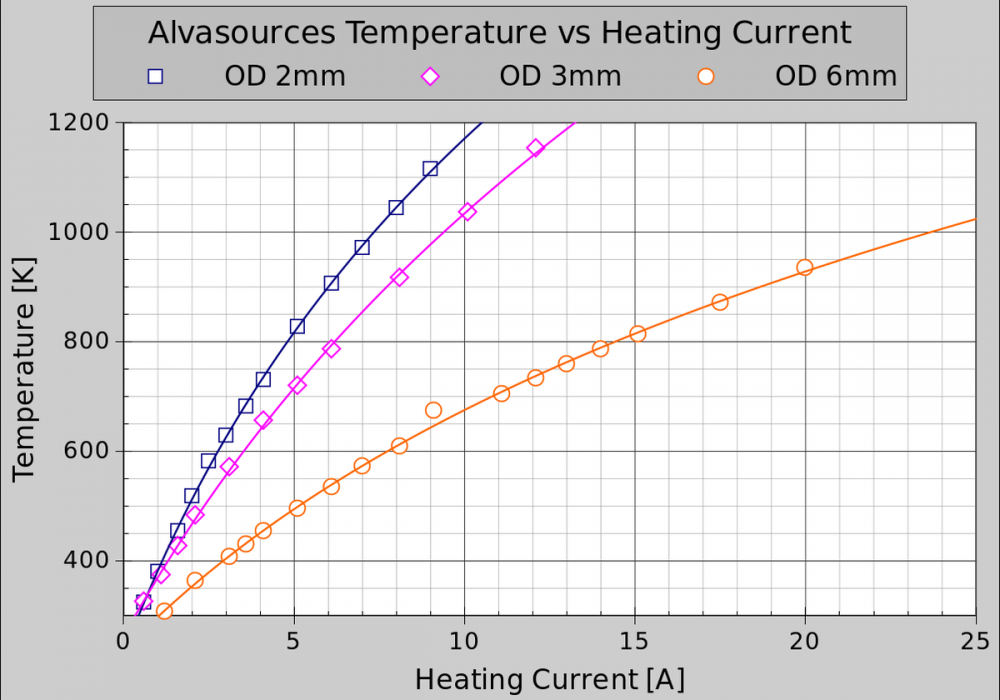
\includegraphics[width = 0.7\linewidth]{figures/Apparatus_dispen.png}
\end{center}
\caption[Temperature-current relationship of dispenser (Image from \href{https://alfavakuo.eu/products/mvs/}{alfavakuo})]{Temperature-current relationship of dispenser (Image from \href{https://alfavakuo.eu/products/mvs/}{alfavakuo}). The dispenser of Na and Rb are both with diameter of 3 mm.}
\label{Apparatus_dispen}
\end{figure}

% CMOT, molasses (done 2021-8-26 14:28:05)
After atoms gradually accumulating within 30 seconds, Na and Rb MOT finally achieves saturation. To avoid collision between Rb and Na that induces an inelastic process, we use a resonance light to push the Rb MOT aside to avoid overlapping Na and Rb. That dual MOT typically can capture $10^{9}$ Rb and $1.5 \times 10^{6}$ Na. To increase its density, we apply a compress-MOT (CMOT) process, which increases the restoring force by far detuning the MOT laser\footnote{in our experiment, we do not increase the magnetic gradient.}. To further increase the phase space density (PSD) of the sample, a molasses process is implemented to cool the sample further. Finally, we load the sample into QT with both species in $\ket{F=1,m_F=-1}$ state.

% In QT and QT evaporation and hybrid trap (done 2021-8-26 14:53:38)
A pair of the anti-Helmholtz coil generates the Quadrupole trap (QT). At the beginning of the time sequence, the magnetic gradient is ramped up to 160 G/cm, served as a conservation trap for capture all atoms from the precooling stage. Then, we do the evaporation cooling for Rb which using a MW to pump atoms from $\ket{F=1,m_F=-1}$ to $\ket{F=2,m_F=0}$. Due to the anti-trapping of $\ket{F=2,m_F=0}$ state, we can remove the high-temperature atoms away from the trap to decrease the overall sample temperature. Na atoms are sympathetically cooled by Rb. Due to Majorana loss bringing anti-evaporation effect, we add a single beam optical trap to shift the minimum position of the whole potential away from the QT centre. This works at the first evaporation stage and helps us obtain a sample with 20 $\mu$K temperature. After that, we adiabatically lower down the QT to 26 G/cm for avoiding severe Majorana loss further. After the MW sweeping to 6833 MHz, we finally achieve a mixture sample with temperature around several $\mu$K. This allows us to load them to an Optical dipole trap to do further cooling and experiment. More details about this hybrid trap can be found in this note of our lab \cite{xiong2013production}.

% In OT and OT evaporation (done 2021-8-26 15:09:24)
Optical trap evaporation is achieved by forcibly reducing the light intensity. In the later stage, the atomic density becomes lower due to the weakening of confinement, which reduces the collision rate, so a slower evaporation rate is required. As a result, the optical trap evaporation is relatively inefficient. Using 1070 crossed OT in our experiment, we typically spend 3 s to obtain a two-species BEC. For a one-dimensional optical trap, the evaporation time requires even longer and may take 5-10s. Therefore, we generally obtain BEC in the 1070 XOT first and then transfer it to other types of optical traps for experiments. Of course, the transfer process will inevitably bring excitation, so it is crucial to deceive an adiabatic process or wait a long enough time for reaching the ground state.

% state preparation (done 2021-8-26 20:11:43)
Since we need the Feshbach resonance between Na and Rb both in  $\ket{F=1,m_F=1}$ state, we need transfer atoms from $\ket{F=1,m_F=-1}$ to the target state. The easiest and most robust way is the adiabatic-rapid passage (ARP). By applying an RF(or MW) field to couple the initial and target state, we can detune its detuning from the blue (red) side to the red (blue) side. Following the dressed state, atoms start from $\ket{F=1,m_F=-1}$ however end with $\ket{F=1,m_F=1}$. This procedure needs enough adiabaticity, which is time-consuming; however, it is robust from the system's power fluctuation and time precision. We carry out the transition under a low magnetic field, which enables us couple the $\ket{F=1,m_F=-1}$ state to $\ket{F=1,m_F=0}$ and then to $\ket{F=1,m_F=1}$. For latter experiments that need $\ket{F=1,m_F=0}$, we can apply a relatively high magnetic field to decouple these two transitions. More details can be found in the previous thesis \cite{WangFudong2016Soau,LiXiaoke2015Chsd,LiLintao2021}.

% 1070 and 946 ODT (done 2021-8-26 15:24:14)
\begin{figure}[htb]
\begin{center}
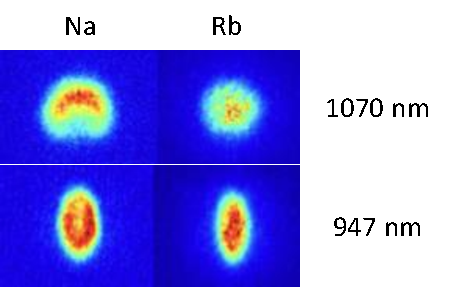
\includegraphics[width = 0.6\linewidth]{figures/OT_1070-946.pdf}
\end{center}
\caption[Na and Rb samples in 946 and 1070 nm ODT (image from \cite{LiLintao2021})]{Na and Rb samples in 946 and 1070 nm ODT (image from \cite{LiLintao2021}). Due to gravitational sag difference, Na in 1070 ODT is buoyant above Rb. In 946 nm ODT, Rb stays at the centre of Na, showing the sag difference's excellent compensation.}
\label{OT_1070-946}
\end{figure}

% BEC mixture (done 2021-8-26 16:49:43)
In our experiment, Na has a relatively large interaction strength $g_{Na}$ (even its scattering length is smaller than Rb, its mass three times smaller than Rb.), so at the beginning of OT evaporation, it is Na sympathetically cooling Rb. However, typically Na becomes BEC before Rb does because of a higher transition temperature, which is mainly due to the higher trap frequency of Na in the 1070 nm ODT. After that, the evaporation is mainly for the Rb sample, and we can achieve a two-species BEC with an almost balanced number at the final. This number ratio actually can be tuned by changing the evaporation ending in QT. For the double BEC sample in ODT, Na is immiscible with Rb in the case of a low magnetic field. Thus, Na shows a crescent shape which is because of the gravitational sag difference of two samples (shown in Fig. \ref{OT_1070-946}). In order to obtain a relatively pure BEC sample, we lower down the optical trap to a relatively shallow level, such as about 80 Hz for Na in 1070 ODT. We check the purity of the BEC sample by observing the BEC sample without any thermal part for whatever ToF. Then, we say that the sample is pure enough. However, to characterize the temperature of this sample, correspondingly the BEC fraction, is typically hard, which is beyond the range of this thesis.

% number ratio control (done 2021-8-26 17:54:39)
In many experiments, we need to control the number ratio of Na and Rb. The typical method is to adjust the optical trap's relative position to the QT's zero-point. By modifying this distance, we can determine the atomic number of Rb after the QT evaporation. Rb will be less evaporated and more Rb atoms remain for a longer distance, vice versa. Because the Na number is much less than Rb, with sympathetically cooled, the Na number mainly unchanges. However, the temperature will be the same as Rb. Subsequently, the evaporation of loading into OT is dominated by Na, as mentioned before. Therefore, the number ratio of Na and Rb can be manipulated by changing the number of the remaining Rb after QT evaporation.

% 946 trap (done 2021-8-27 10:40:15)
As described in \cite{LiLintao2021}, we build an optical trap with magic wavelength, which offers the same trap frequency for both Na and Rb. As shown in Fig. \ref{OT_1070-946}, Rb stays at the centre of Na. We can benefit a lot from this wavelength, such as increasing the overlap between Na and Rb and consequently increasing the Feshbach molecule's conversion rate or enhancing the signal of the polaron experiment. Our droplet experiment uses this sag-difference-free trap to achieve better overlap and form droplets with lower density and longer lifetime, which will be discussed in Chap. \ref{Chap_droplet}.

\subsection{Producing Na-Rb Feshbach molecules}
% motivation (done 2021-8-26 18:49:35)
In our laboratory, the original intention of producing Feshbach molecules is to make the ground state molecule of NaRb further. After successfully making the ground state molecule \cite{PhysRevLett.116.205303}, the mission of this machine becomes the study of heteronuclear mixture BEC. The core ingredient of research on this set-up consequently involves adjusting inter-particle interaction through the Feshbach resonance. Many interesting physics problems can be studied, such as Effimov state, polaron, spinor. Then the essential parameter is the FR parameter, i.e. how the scattering length of the inter-species changes with the magnetic field. The detailed calibration and calculation will be demonstrated in Chap. \ref{Chap_Feshbach}. We note that the scattering properties near resonance will be most affected by the shallowest bound state, so the precision measurement of the bound state will give accurate scattering properties in turn. Therefore, we need to synthesize FR molecules and study their properties.

% method (done 2021-8-27 10:40:51)
Our experiment starts from an optically trapped ultracold mixture of $^{23}$Na and $^{87}$Rb atoms, both in their lowest hyperfine state $\ket{F = 1, m_F = 1}$~\cite{wang2013observation,wang2015formation,jia2020}. Magnetoassociation starts from an initial magnetic field of 350 G, just above the FR at $B_0 = 347.64$ G. The magnetic field is ramped down across the resonance to form FMs, and then to 335.6 G. At this field, the FMs have a nearly zero magnetic dipole moment; this allows us to remove the residual atoms with a short and strong magnetic field gradient without losing molecules. Afterwards, the magnetic field is ramped up to a range of target values below $B_0$ for further experiments. Following this procedure, we can routinely obtain a pure sample of $^{23}$Na$^{87}$Rb FMs with a typical temperature of 300 nK and a trap lifetime of more than 30 ms. This short lifetime is due to near-resonance photon scattering by the 947 nm optical trap light~\cite{Guo2017,jia2020}, which is provided by a home-built diode laser system. In another experiment on $^{23}$Na$^{87}$Rb, in which a single-frequency 1064 nm laser is used as the optical trap light, FM lifetimes greater than 100 ms have been observed~\cite{Wang2019,guo2021leehuangyang}. Nevertheless, the current lifetime is more than enough for the present work, as we need only 10 ms for magnetic field stabilization and less than 1 ms for dissociation.

\section{Image system upgrades}
\label{sec:image}

% motivation: why upgrade image system (done 2021-8-27 11:04:57)
The previous image system is composed of an f=100mm (\#49360-INK) and f=300 mm (\#49368-INK) pair from Edmund optics, which can support a resolution of about 3 $\mu$m (N.A.=0.13) as shown in Fig. \ref{old_image}. This imaging system is built with discrete elements, which cannot move
as a whole. Thus, it is only proper for imaging for a small region; otherwise, both spherical aberration and coma shows up if moving only the camera or the lens set. We need to do the ToF for samples for the droplet experiment, and the displacement reaches about 2 mm. If we change the camera position, the resolution for imaging sample with large displacement, i.e. at the edge of field-of-view, will be degraded. So, we improved our resolution by two means: First, we increase the imaging system's resolution by using a long working distance objective; secondly, we build a whole block by mounting all optical elements and cameras onto an electric translation stage. In the rest of this section, we discuss the absorption image method for a dense atomic cloud, introduce a high-magnetic-field image scheme, and discuss the number calibration method.

% old imaging system (done 2021-9-16 17:21:13)
\begin{figure}[htbp]
\begin{center}
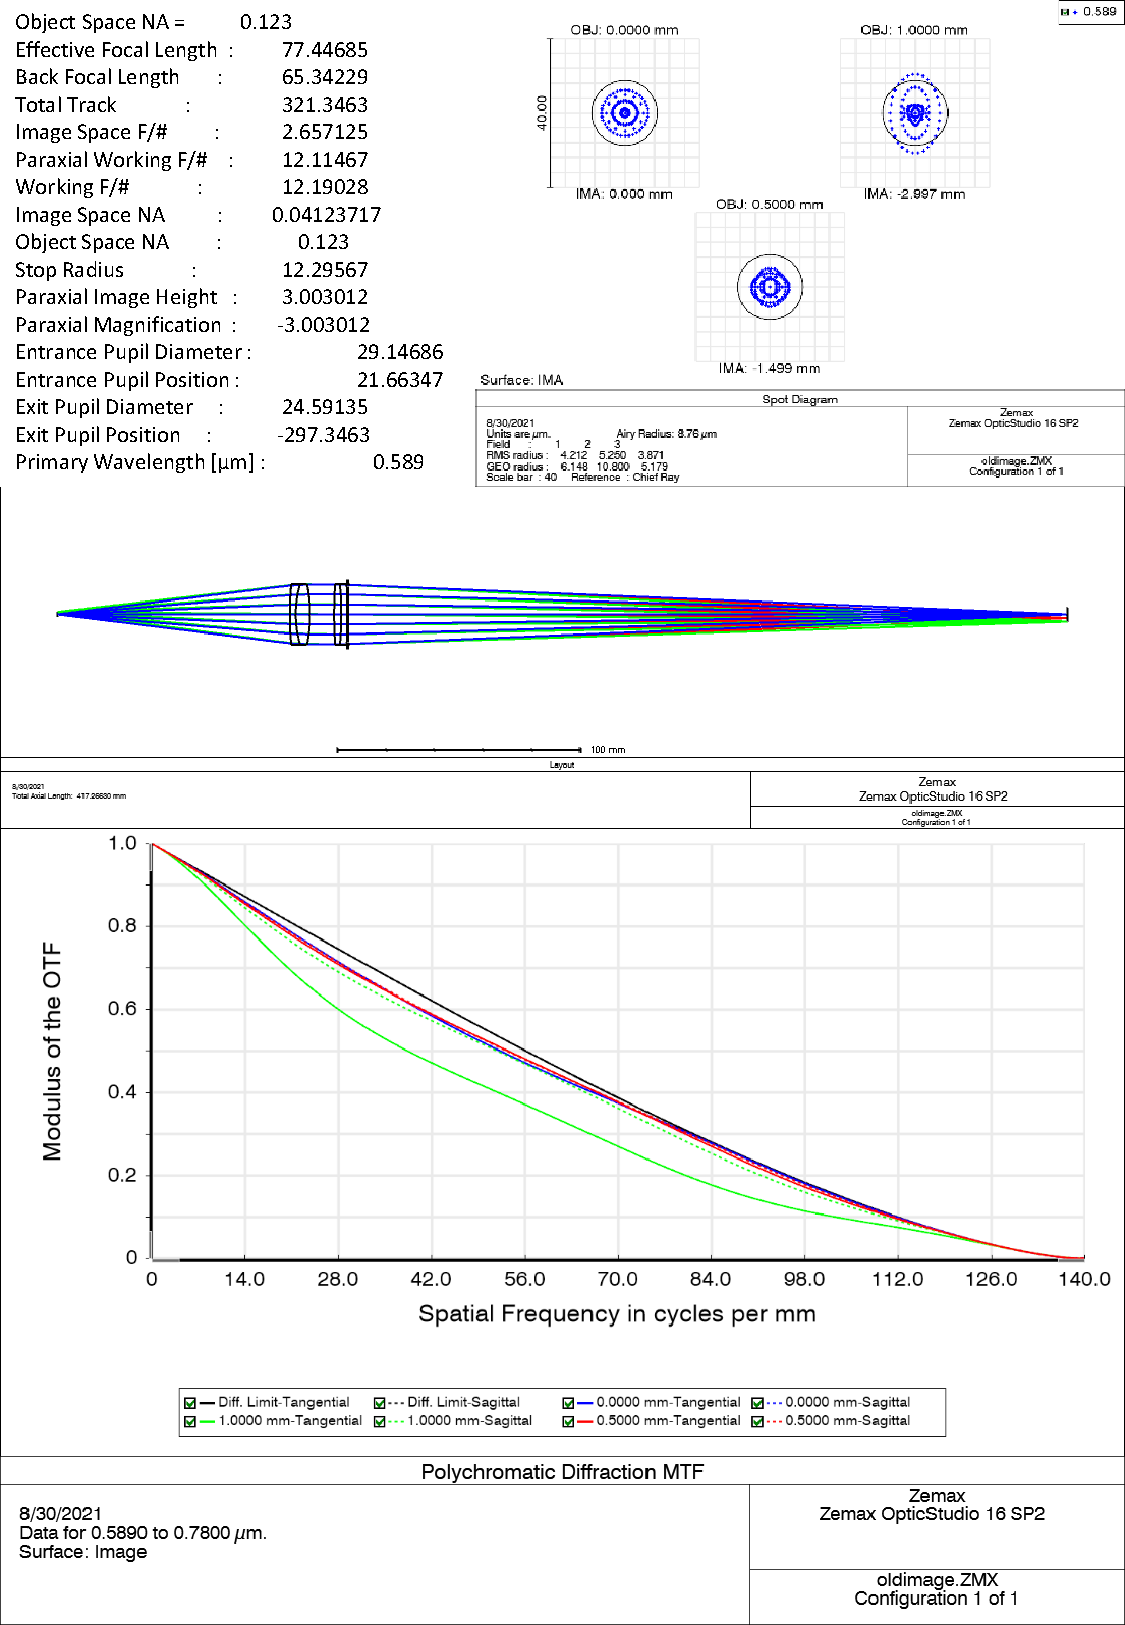
\includegraphics[width = \linewidth]{figures/old image.pdf}
\end{center}
\caption[3x image system simulation by Zemax]{3x image system simulation by Zemax. From the spot diagram and MTF calculation, we can read out a large field-of-view of this system.}
\label{old_image}
\end{figure}

\subsection{High resolution image system}

% optical design (done 2021-8-27 14:44:36)
The characteristic length for a droplet is typical of several $\mu$m, as shown in Sec. \ref{Chap_droplet}. In order to resolve this tiny sample, we need a better imaging system with resolution reaching $\mu$m level. The old imaging system with an f=100mm objective is not enough since its N.A. is 0.13 with an airy radius of about 4 $\mu$m. So, we use an objective with a shorter focal length to increase N.A. The most convenient way is using a microscope with a long working distance. So, we choose a 10X Mitutoyo plan-apo infinity-corrected Long-WD objective with an effective focal length of 20 mm. Its working distance reaches 34 mm, enough for our application without blocking any optical path, such as MOT or optical trap. We can use the same eyepiece (Edmund \#49368) with f=300 mm and directly image the atom onto the camera thanks to the infinity-correction property. 

% mechanical design (done 2021-8-27 15:09:52)
As shown in Fig. \ref{image_system}, We use the cage system from Thorlabs to build the main body of the imaging system. A $45^\circ$ mirror reflects the probe beam in the vertical direction. This avoids the diffraction light from optical dipole trap scattering to CCD and affects the image quality. The dichromatic mirror can be tuned to ensure the Na image is at the centre of Na CCD. Moreover, we add a ring adjuster for Rb CCD to fine-tune its position. This is mainly for focusing on both Na and Rb. Because there always be a chromatic shift for two different wavelengths (589 nm for Na and 780 nm for Rb). So, when focusing on the system, we first focus the Na by move the set-up as a whole, i.e. move the objective on focus to the atom. Then, we tune the ring adjuster to focus Rb onto the camera. One mistake is that we choose an adjuster too fine (4 mm for ten turns), so the adjustment procedure typical take a long time. As mentioned before, the whole system is mounted onto an electric translation stage controlled by an Arduino. Code and control can be found in Lintao's thesis \cite{LiLintao2021}.

% High-field image scheme (done 2021-8-27 15:12:52)
\begin{figure}[htb]
\begin{center}
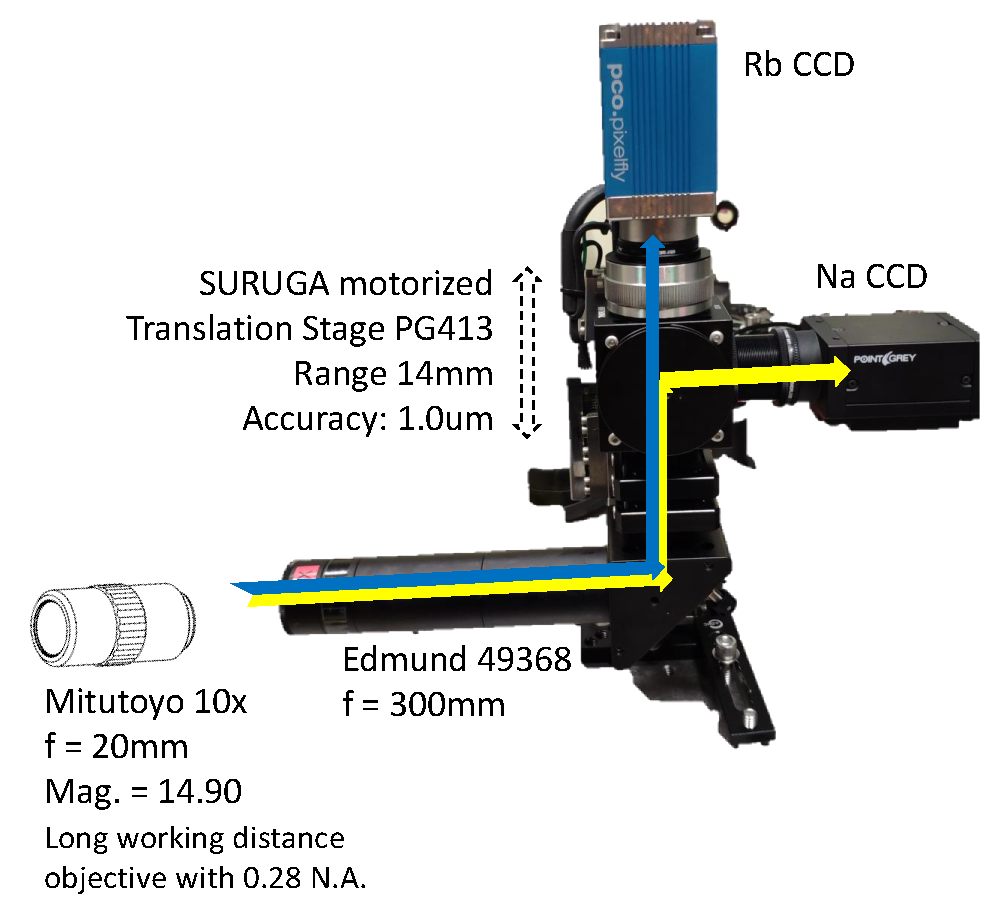
\includegraphics[width = 0.8\linewidth]{figures/image_system.pdf}
\end{center}
\caption[New compact imaging system]{New compact imaging system. The whole set-up is mounted on a electric translation stage from SURUGA. The objective can be switched between a Mitutoyo 10x microscope and a typical f=100 mm achromatic lens. Then follows a f=300 mm eyepiece for focusing. A dichromatic mirror splits Rb and Na probe into two CCDs.}
\label{image_system}
\end{figure}

% cell wall effect (done 2021-8-27 15:35:56)
Even though we use a powerful objective with an Airy radius of 1 $\mu$m, there exists a critical issue that the cell wall is 3 mm thick. So, we need to check the imaging system's performance with this 3 mm window before the objective. We did not do any correction for this glass wall because our primary goal is to increase the magnification. Even the resolution only increase twice will be enough for observing droplet signals. The 3 mm window will decrease the resolution\footnote{A tutorial for standard object correction ring can be found \href{ http://www.mvi-inc.com/wp-content/uploads/Use-of-the-Correction-Ring-on-the-Objective.pdf}{here}. Moreover, the effects of thick glass on an imaging system can be found on \href{https://www.thorlabs.com/newgrouppage9.cfm?objectgroup_id=9895&pn=TL2X-SAP}{Thorlabs} under the tag of correction collar}. Since when the focused beam goes through the glass wall, light with a different angle will bend by different amplitude and finally, they cannot converge to a single point as without the glass. This effect is severe when the N.A. goes higher.

% resolution test (done 2021-9-16 19:04:44)
\begin{figure}[htb]
\begin{center}
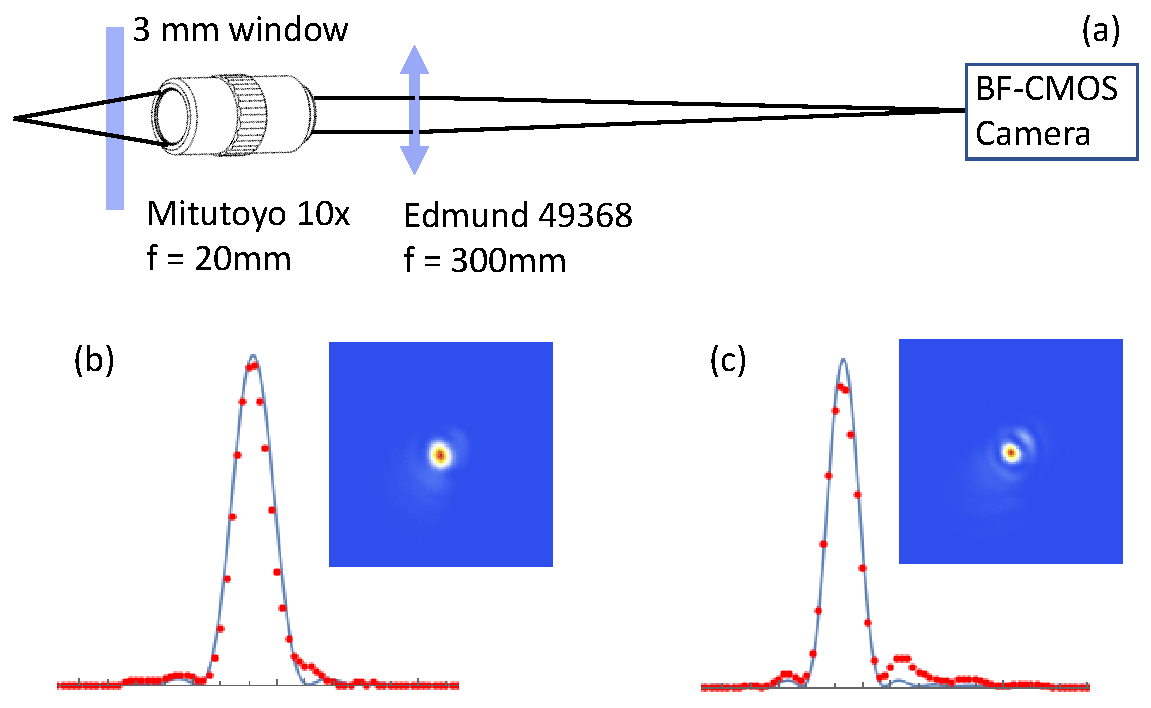
\includegraphics[width = 0.9\linewidth]{figures/Apparatus_image-reso.pdf}
\end{center}
\caption[Image resolution test of 15x image system]{Image resolution test of 15x image system. (a) shows the test method. a 2 $\mu$m pin-hole is used as target. Image is taken be a pixel-size 3.45 $\mu$m Blackfly CMOS camera. (b) and (c) shows the airy disk we measured for Rb and Na.}
\label{image_reso}
\end{figure}

% test resolution (done 2021-8-27 15:49:18)
Before putting it online, we first test its resolution offline with a USAF1951 target and 2 $\mu$m pinhole. Here, we show the measured Airy disk in Fig. \ref{image_reso}. By simply fitting the pattern with the Airy function, we get the resolution for Na(Rb) is 1.7(2.3) $\mu$m. So we now have a high resolution and commercial and cheap image system. 

% Translation stage (done 2021-8-27 16:44:06)
Because we will do ToF measurement for several tens of ms, i.e. about 2 mm away from the centre of view-of-field, spherical aberration and coma can worsen the image quality. This can be shown by Zemax by a tilted angle of input light (Fig. \ref{image_reso}). We use a high magnification imaging system with a short focal length of 20 mm. This makes its field-of-view very small. So, we need to move the whole imaging system along with the atomic sample. So, we build the imaging system very compact and mount it onto a translation stage controlled by a computer. The translation stage is mounted vertically with a step resolution of 1 $\mu$m. We use an Arduino board to control the driver. Finally, we can change the position of our image system at will shot by shot. To avoid the movement changing affecting the EM field around the cell, we make each movement at the interval of two shots.

\subsection{High magnetic field absorption image}
\label{subsec:high_mag_absop_image}

% goal (done 2021-8-27 16:47:15)
To probe the droplet without distortion, we need the imaging scheme reliable, which means the method can recover the density profile of the sample as accurate as possible. Since a typical droplet sample has OD above 50 for Rb and 10 for Na, a typical absorption image method cannot be used directly, which is because the absorption image's SNR is limited when the sample OD is too high. As plotted in Fig. \ref{SNR_OD}, weak probe intensity (less than one saturation intensity) can only support OD smaller than 3 \cite{guo2021SNR}. Increasing the probe intensity to achieve the saturation absorption image can increase the threshold of OD to probe. However, higher intensity could cause several other problems: first, calibration could be hard to do or cause a significant error because the nonlinear response of the absorption. second, for a high density sample the re-scattering problem could introduce the effect beyond the aforementioned theory. So, we conceive a partial pumping method and a high-magnetic field absorption imaging scheme for the high-OD samples.

% SNR of absorption image as a function of OD (done 2021-9-18 15:21:00)
\begin{figure}[htb]
\begin{center}
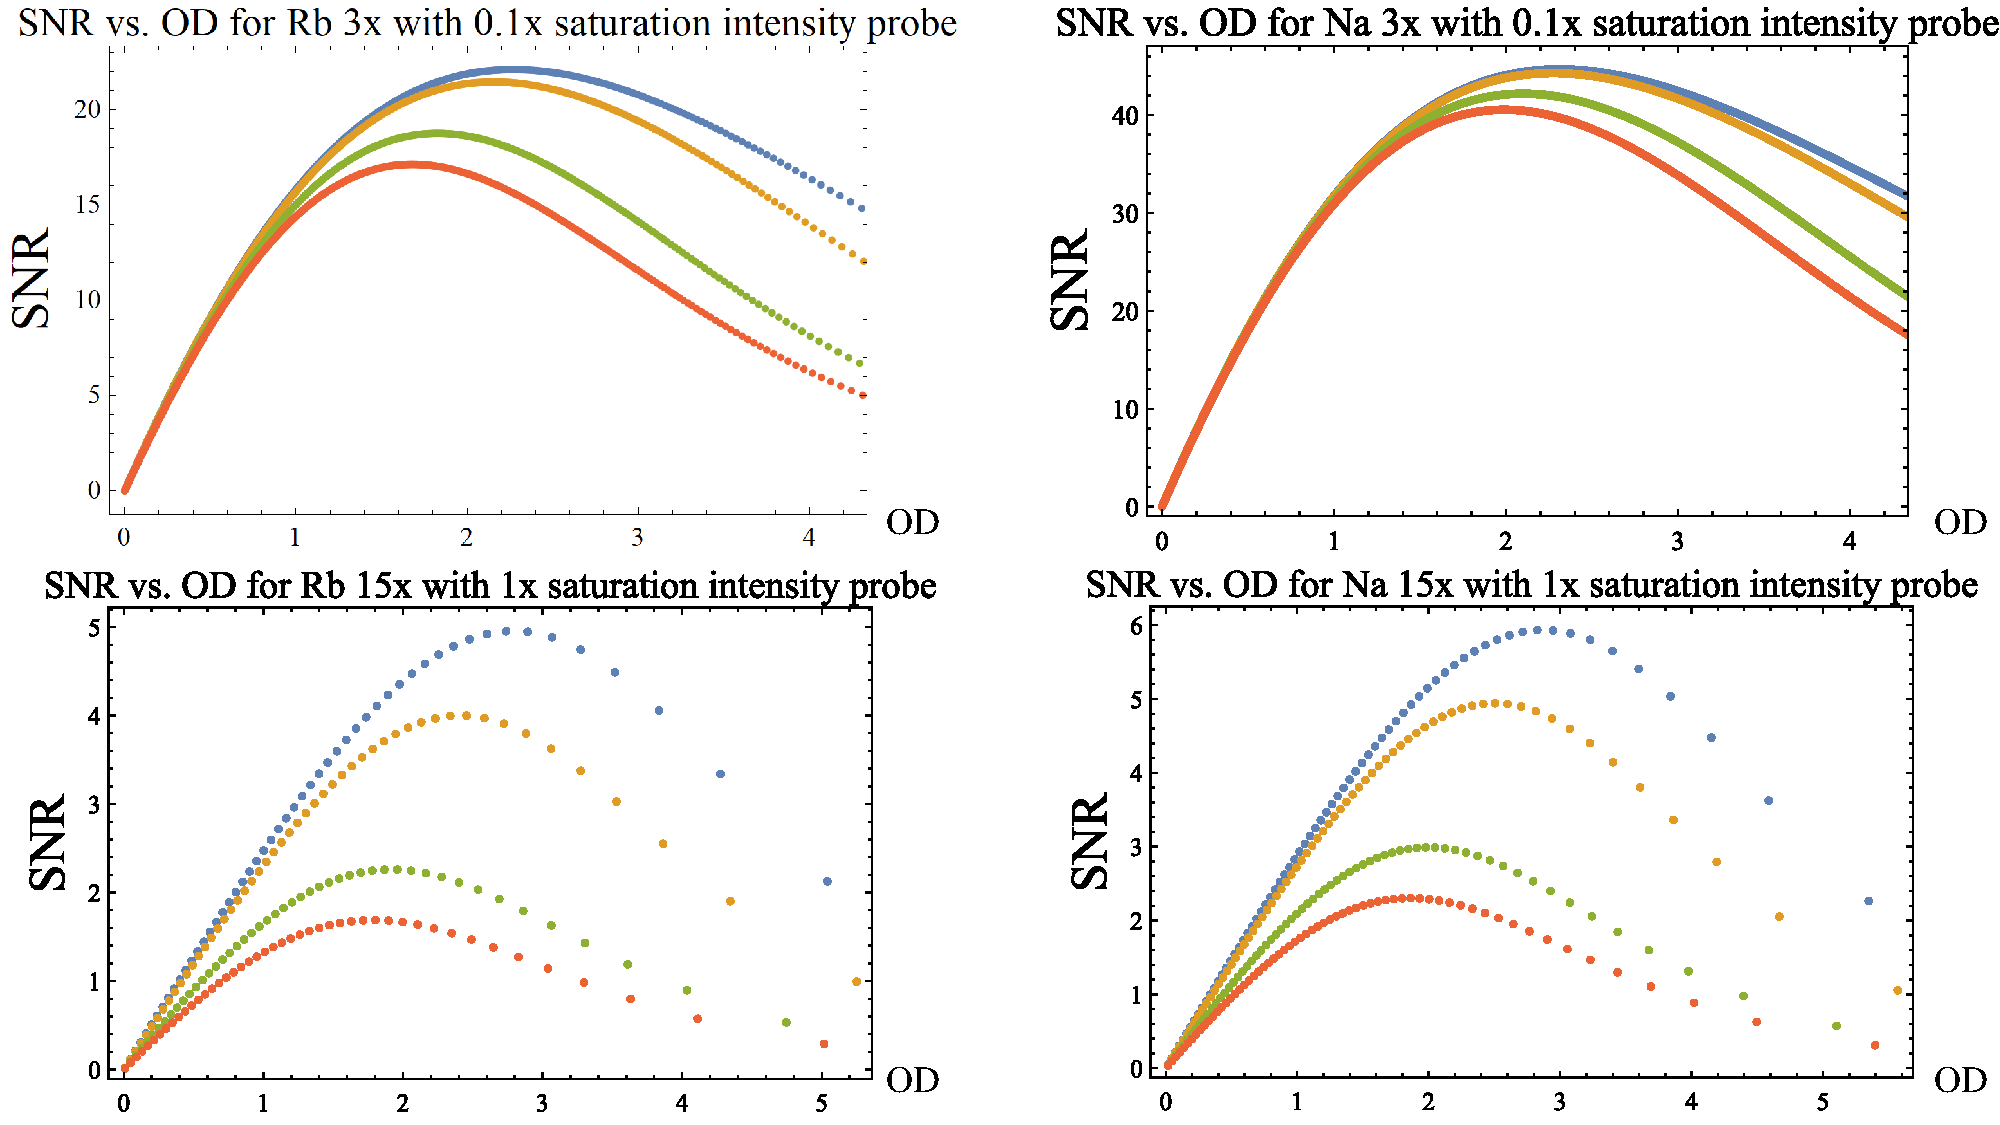
\includegraphics[width = \linewidth]{figures/Apparatus_AI_SNR.pdf}
\end{center}
\caption[SNR of absorption image as a function of OD]{SNR of absorption image as a function of OD. Above two panels are our 3x image system, and Lower two panels are our 15x image system. Blue dots for PCO-sCMOS camera; yellow dots for BFS-PGE-31S4; green dots for PCO double-image camera; orange dots for Pointgrey 51S5.}
\label{SNR_OD}
\end{figure}

% image scheme (done 2021-8-27 17:47:45)
Thus, we first decrease the sample's density; however, we keep its profile unchanged. Then, we apply the typical absorption image. This is what we called the partial pumping method for absorption image. A typical way to pump a small portion of the sample to the image transition is by MW or light. As shown in Fig. \ref{image_system}, our sample is at $\ket{F=1,mF=1}$ state, which is non reacting with the absorption light. Then, we use a pumping laser to pump atoms to exited state $\ket{m_J=1/2,m_I=3/2}$; then, with spontaneous radiation, atoms accumulate onto $\ket{F=2,m_F=2}$ state. Finally, we use the cycling transition from this state to $\ket{m_J=3/2,m_I=3/2}$ state to do the absorption image. Here the pumping can also be done by the MW pulse. However, our original MW had a Rabi freq less than 10 kHz, which could consume 100 $\mu$s or even longer apply a $\pi$ pulse. This would make the sample's shape changed a lot when we probe it by the image light. We will get back to this point when we discuss our upgrades of the Full-wave loop-antenna in Sec. \ref{subsec:FWLA}. 

% High-field image scheme (done 2021-8-27 16:52:34)
\begin{figure}[htbp]
\begin{center}
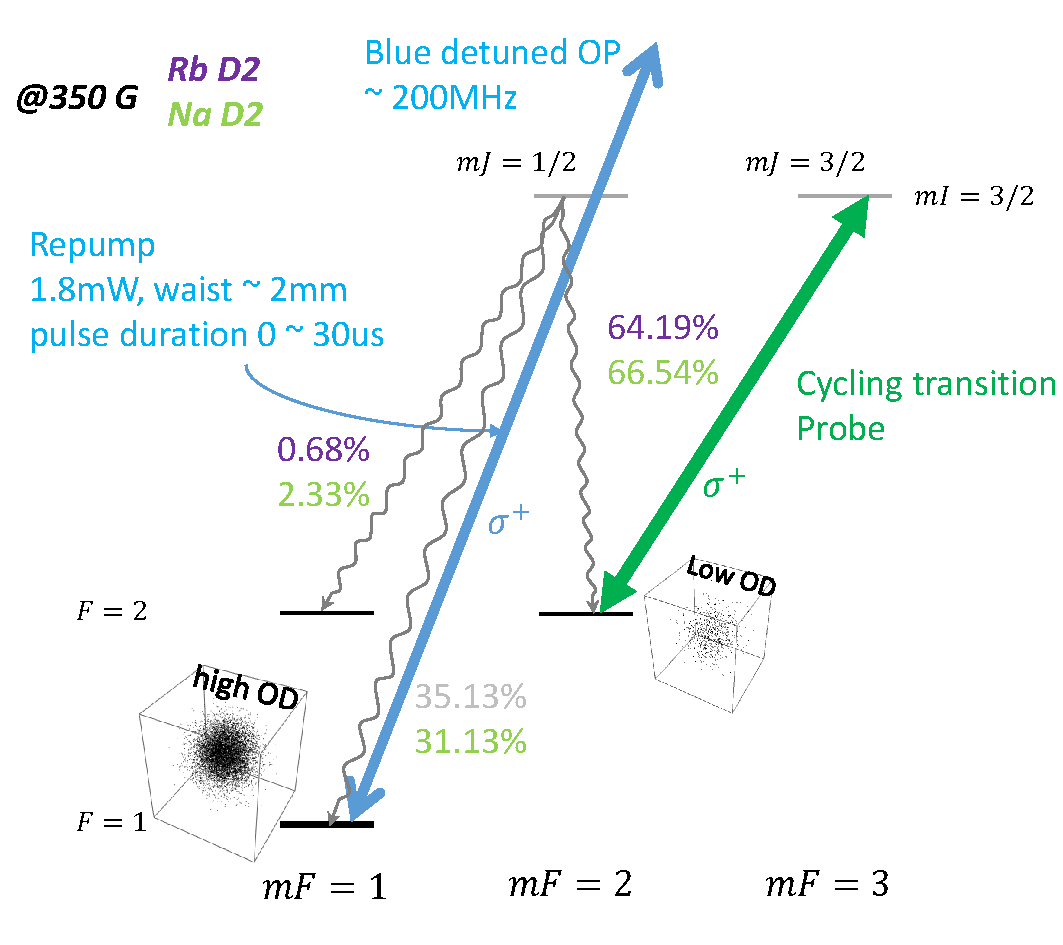
\includegraphics[width = 0.8\linewidth]{figures/High-field image scheme.pdf}
\end{center}
\caption[image scheme for Na(Rb) $\ket{F=1,m_F=1}$ state under 350 G magnetic field]{image scheme for Na(Rb) $\ket{F=1,m_F=1}$ state under 350 G magnetic field. The ground states are labelled with F and $m_F$; the excited states are labelled with $m_J$ and $m_I$. The imaging procedure is divided into two steps: first, pumping atoms from $\ket{F=1,m_F=1}$ to $\ket{m_J=1/2,m_I=3/2}$. After atoms accumulating to $\ket{F=2,m_F=2}$ state, we drive the cycling transition for absorption image. By blue detuning about 200 MHz of the pumping light, we can control the pumping ratio to control the OD for the image transition.}
\label{High-field image sheme}
\end{figure}

% partial pumping (done 2021-8-27 18:02:39)
So, we choose the pumping laser instead of tuned to on resonance, and we make it large detuned away from the transition and make its intensity high. This method ensures the whole sample feel around the same intensity because large detuning and intensity make the atoms only absorb a tiny portion of the light. Even for a very dense sample, the unevenness of the saturation effect can be avoided. As plotted in Fig. \ref{High-field image sheme}, Na partial pumping a small portion of the sample to $\ket{F=2,m_F=2}$ state, which then can be detected directly. The pumping ratio can be controlled by the duration of the pumping laser. As shown in Fig. \ref{partial pumping}, the OD of pumped Na atoms as a function of the pumping duration is plotted. We can see that we have an almost linear pumping speed for the first several tens of us, and after 50 $\mu$s we have a saturation effect. This saturation effect is used to calibrate latterly. For our experiment, to decrease the OD to less than 3, we typical using a detuning 200-300 MHz and pumping only several $\mu$s to achieve a portion less than 10 per cent. Then a typical low-intensity absorption image can afford it.

% partial_pumping (done 2021-8-27 17:50:32)
\begin{figure}[htb]
\begin{center}
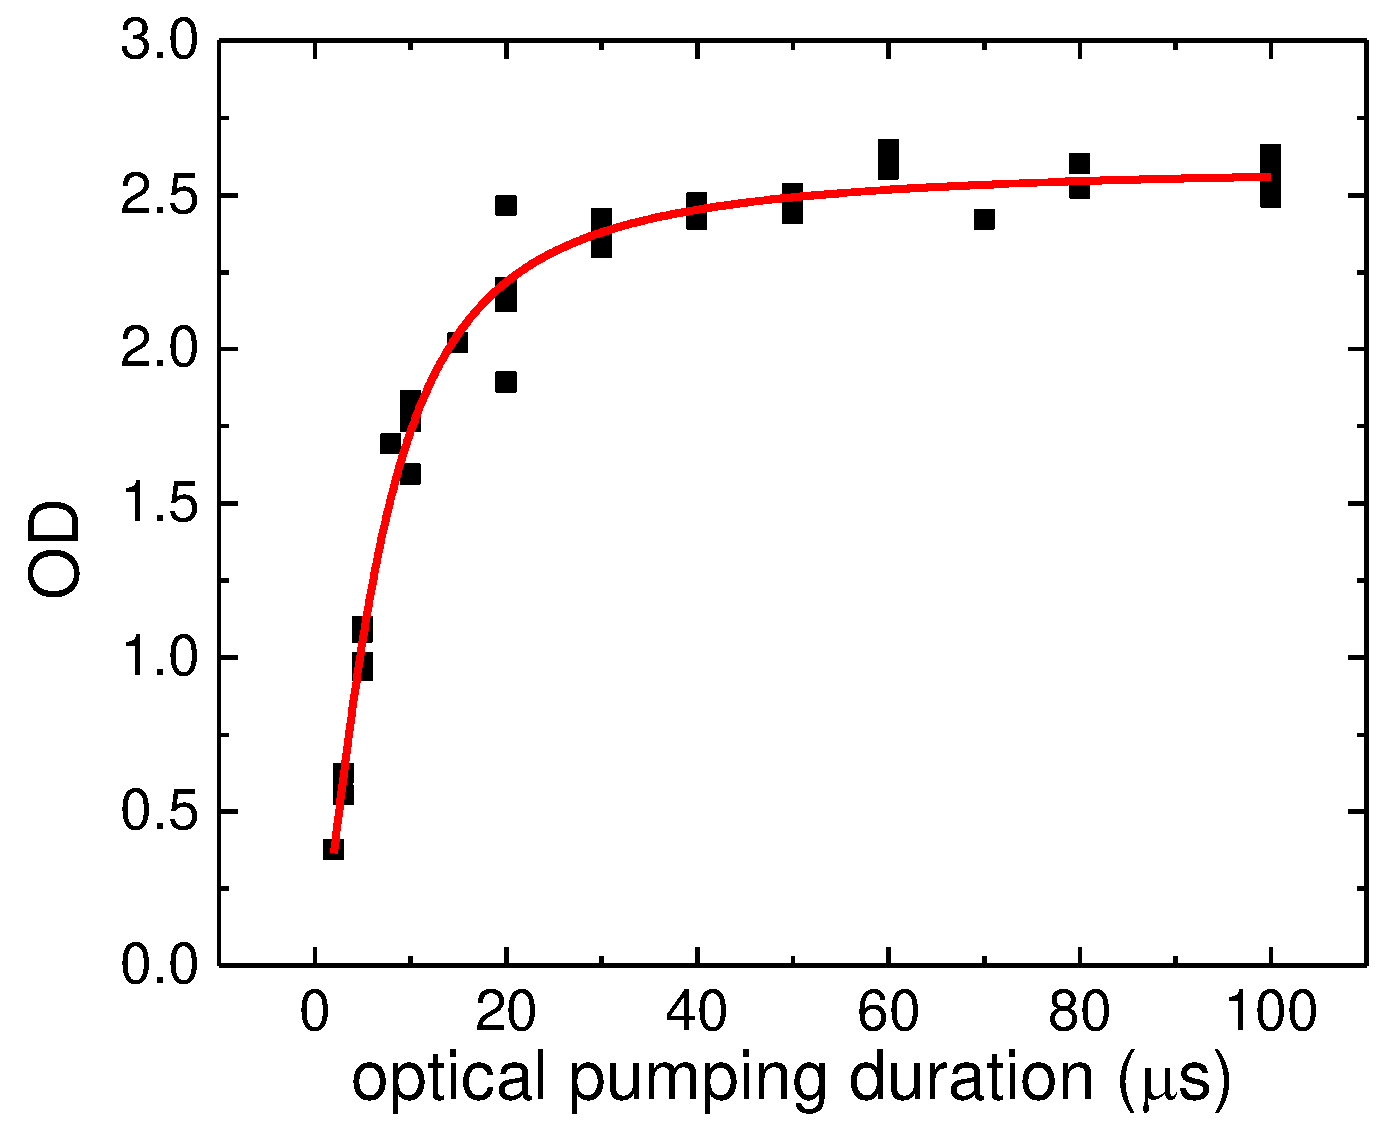
\includegraphics[width = 0.8\linewidth]{figures/partial_pumping.pdf}
\end{center}
\caption[Partial pumping portion as function of pump duration]{Partial pumping portion as a function of pump duration. Here shows the partial pumping for Na with 200 MHz blue detuning of the pumping light.}
\label{partial pumping}
\end{figure}

\subsection{Atomic number calibration}

% overall and method(done 2021-9-20 11:47:23)
In the previous subsection \ref{subsec:high_mag_absop_image}, in order to perform absorption imaging on samples with higher optical density (OD), we use the partial pumping method to reduce its OD. However, in order to ensure the signal-to-noise ratio of the imaging, we usually do not use the probe light whose intensity is much smaller than the saturation intensity. Therefore, considering that the droplet experiment requires atomic number measurement, we need to do a more careful atomic number calibration for our high field absorption imaging. The principle of calibration is mainly derived from the calibration of several parameters in absorption imaging. For now weak probe light intensity, the expression of absorption imaging is
\begin{equation}
\frac{dI(x,y)}{dz}=-n(x,y,z)\sigma_{eff}(\delta,I,others)I(x,y)
\end{equation}
In above formula, $\sigma_{eff}$ represents the effective cross-section of atoms, which is related to probe detuning, intensity and other parameters such as polarization. By separating intensity and detuning, we have
\begin{equation}
\sigma_{eff}(\delta,I,others)=\frac{\sigma^*(others)}{(1+(\frac{2\delta}{\Gamma})^2)+\frac{I}{I^*_{sat}(others)}}
\end{equation}
Probe light transmits along the $z$ direction and has a distribution in $x$-$y$ plane. $n(x,y,z)$ is density distribution of a bulk sample. When we do absorption image, we actually probe the column density
\begin{equation}
\label{sat_absorp_formula}
\int n(x,y,z)dz=\frac{OD(x,y)}{\sigma^*(others)}=\frac{1}{\sigma^*(others)}[ln(\frac{I_{in}}{I_{out}})+\frac{I_{in}-I_{out}}{I^*_{sat}(others)}]
\end{equation}
Thus, in the following calibration, we mainly calibrate two parameters: $I^*_{sat}(others)$ and $\sigma^*(others)$.

% calibrate saturation intensity: beta (done 2021-9-20 23:29:58)
First, we follow \cite{reinaudi2007strong} to calibrate $I^*_{sat}(others)$, which we called it $\beta$-calibration. We define
\begin{equation}
I^*_{sat}(others)=\beta I^0_{sat}
\end{equation}
where $I^0_{sat}=\frac{\hbar \omega A_{21}}{2 \sigma_0}$ is the ideal saturation intensity. To calibrate the beta, we use different camera light intensities to probe the same sample and then directly plot the od without correlation, i.e. $ln(\frac{I_{in}}{I_{out}})$. As shown in Fig. \ref{Image_beta_calibration}, the y-axis represents the counting rate of probe light which is proportional to light intensity $I_{in}$; x-axis is the od without correction we mentioned before. Via formula \ref{sat_absorp_formula} We can fit this curve and then get $CR_{sat}^{eff}$. We use counting rate instead of light intensity, mainly because CR can be read directly on the camera. Using the effective saturated CR to obtain the corrected od is more directly than using $\beta$. In other words, for the correction of imaging, we don't actually care about the value of $\beta$, and it is actually enough to have saturated CR. Finally, in Table. \ref{tab:image_cali}, we offer the effective saturated CR  of Na and Rb in the two different image systems we used. At the same time, we point out here that the $\beta$ value depends on various parameters, including light polarization, camera parameters, projection parameters of the imaging system, etc. Therefore, the number calibration of each system should be done separately. Through this engineering method, all unexpected parameters are absorbed into a single variable.

% Image_beta_calibration (done 2021-9-20 14:11:12)
\begin{figure}[htb]
\begin{center}
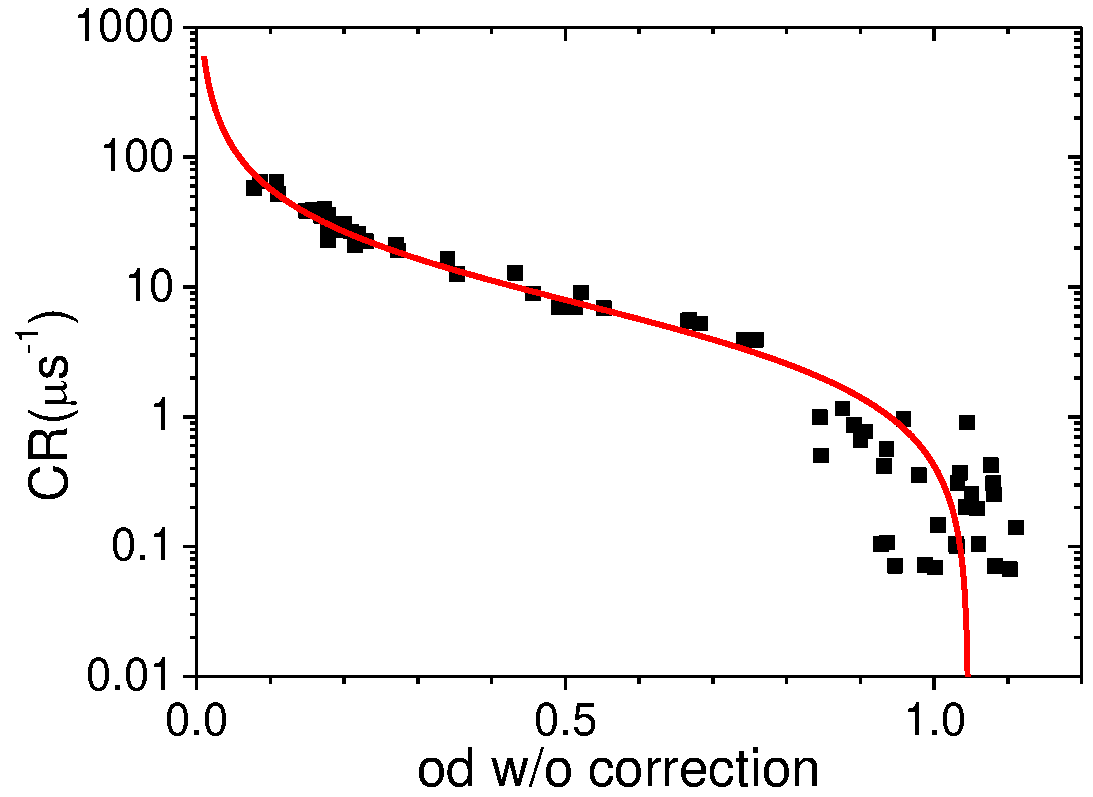
\includegraphics[width = 0.8\linewidth]{figures/Image_beta_calibration.pdf}
\end{center}
\caption[$\beta$-calibration of Rb 15x absorption image]{$\beta$-calibration of Rb 15x absorption image. CR is counting rate, i.e. average counting over probe duration. od w/o correction is $ln(I_{in}/I_{out})$ without correcting the saturation effect.}
\label{Image_beta_calibration}
\end{figure}

% calibrate alpha (done 2021-9-20 23:38:36)
The above calibration for saturated light intensity avoids the OD change of the sample from different probe intensities. However, considering the expression \ref{sat_absorp_formula}, in order to obtain the column density distribution of the sample, we also need an effective scattering cross-section $\sigma_{eff}$. In order to obtain this parameter, we need to compare the OD obtained by absorption image to the column density of the actual atom density distribution. The point to be emphasized here is that we do not use the parameters in the $\beta$-calibration to correct the cross-section because of light imperfection, such as polarization, etc. The two are not entirely consistent. On the other hand, we use the partial pumping method. Therefore, we hope that this effective cross-section parameter can absorb the imperfection of pumping, such as leakage to the other states, which does not result in 100\% pumping. We put this part of the calibration into the alpha. This part will not affect the saturation intensity of the probe but will affect the number of atoms counted at the end.

% methods of alpha calibration (done 2021-9-21 08:59:23)
For $\alpha$-calibration, we define
\begin{equation}
\sigma^*(others)=\frac{1}{\alpha} \sigma^0_{sat}
\end{equation}
Two methods can be used: one is from \cite{hung2011situ}, which directly compare the density distribution of BEC in-trap with, and directly compare the density distribution of the atom calculated by trap freq with the OD distribution obtained from the photo to obtain the corresponding $\alpha$-coefficient. The other is the number of atoms obtained through the BEC-thermal phase transition and the thermal part's temperature measurement. The corresponding alpha coefficient is obtained by comparing the total OD measured by the photo. The former method is more feasible for a sample with a larger in-trap size because the in-trap sample is typical $\mu$m level, which is difficult to avoid the impact due to the imaging resolution. The latter method can avoid this problem because the measurement of the total atomic number can be obtained from longer ToF. Therefore, in our experiment, we finally adopted the latter one.

% 待补充
% method BEC-thermal transition
% BEC-thermal的phase transition和原子数以及温度的关系是

% summary (done 2021-9-23 11:58:33)
In general, through the above two steps, we can accurately obtain the density distribution of the atom. Adding the high-field imaging method introduced in the Subsec. \ref{subsec:high_mag_absop_image}, we finally offer a complete imaging plan for the droplet experiment. This solution is also suitable for in-situ imaging samples with relatively high OD, such as in-trap BEC, bright solitons, etc. Furthermore, achieving enough resolution by upgrading the imaging system is essential as another aspect of the requirement to retrieve density distribution.

% CR and alpha table (done 2021-9-23 11:58:46)
\begin{table}[]
\begin{tabular}{|l|l|l|l|l|l|l|l|l|}
\hline
   & \begin{tabular}[c]{@{}l@{}}Image\\ system\end{tabular} & \begin{tabular}[c]{@{}l@{}}Mag.\\ field\end{tabular} & \begin{tabular}[c]{@{}l@{}}Probe\\ polar.\end{tabular} & \begin{tabular}[c]{@{}l@{}}OP\\ det.\end{tabular} & $CR_{sat}^{eff}$ & \begin{tabular}[c]{@{}l@{}}$I_{sat}$\\ (mW/$cm^2$)\end{tabular} & $\beta$ & $\alpha$ \\ \hline
Rb & 3x                                                     & LF                                                       & Circular                                               & 0 MHz                                             & 87(4)       & 2.792                                                           & 1.67    & 1.59     \\ \hline
Rb & 15x                                                    & HF                                                       & Horizo.                                                & 0 MHz                                             & 5.7(3)      & 5.421                                                           & 3.25    & 3.75     \\ \hline
Rb & 15x                                                    & HF                                                       & Horizo.                                                & 215MHz                                            & 5.7(3)     & 5.421                                                           & 3.25    & 4.54     \\ \hline
Na & 3x                                                     & LF                                                       & Circular                                               & 0 MHz                                             & 288(5)    & 5.862                                                           & 0.95    &          \\ \hline
Na & 15x                                                    & HF                                                       & Horizo.                                                & 140 MHz                                           & 24(1)     &                                                                 &         & 3.76     \\ \hline
\end{tabular}
\caption[Summary of image calibration]{Summary of image calibration}
\label{tab:image_cali}
\end{table}


\section{CAMIMA: a multi-camera and image process platform}
\label{sec:camima}

% What is CAMIMA and why we need to develop it? (done 2021-8-27 18:27:20)
CAMIMA is a multi-camera control platform with image processing functions. Thanks to various camera adaptors provided by the Image Acquisition Toolbox in MATLAB, CAMIMA can support multiple types of camera, including USB cameras from PointGrey, PCO and Migtex, Web camera and other general type of cameras. The primary time sequence is tailored for the absorption image for the cold atom experiment. However, it is very convenient to switch to other sequences such as fluorescence imaging. After acquiring images from the camera, there are extendable and programmable image processing functions for post-processing images. Users can easily re-program the time sequence and processing sequence for various scenarios, e.g. denoising or de-fringe process, fluorescence image and so on.

% components description (done 2021-8-27 18:41:59)
The software is made of four parts: 
\begin{itemize}[noitemsep,topsep=0pt]
\item CAMIMA: Main control for converting data from different camera to a uniform image stream, which easier for following processing.
\item VUIMA: For showing and processing images from each image stream. VUIMA can be opened multiple.
\item CAMSET: Setting program for various cameras. Inside it, there is a general setting panel adaptation for specific type of camera.
\item FITSET: For general purpose fitting progress. fitting function can be edited as will.
\end{itemize}

\subsection{licensing, versions and updates}
% licensing (done 2021-8-27 18:42:40)
This programs is a free software: you can redistribute them and/or modify them under the terms of the GNU General Public License, version 3, as published by the Free Software Foundation. The full text of the license is available from \href{https://www.gnu.org/licenses/}{https://www.gnu.org/licenses/} and is included in the file COPYING included in the distribution.

% Version control (done 2021-8-27 18:42:47)
For adapting different version of MATLAB and its Appdesigner toolbox, CAMIMA can run under following versions:
\begin{itemize}[noitemsep,topsep=0pt]
\item MATLAB2016
\item MATLAB2020
\end{itemize}

% download and updates (done 2021-8-27 18:42:51)
Software downloads and updates are made available via github:
\begin{itemize}[noitemsep,topsep=0pt]
\item \href{https://github.com/guozc12/CAMIMA}{https://github.com/guozc12/CAMIMA}
\end{itemize}

\subsection{Using the software: a basic guide}
\subsubsection{Prerequisites}
% prerequisite (done 2021-8-27 18:43:49)
Before installing CAMIMA, one need to install MATLAB with a version later than 2016. The listed several add-ons are needed.
\begin{itemize}[noitemsep,topsep=0pt]
    \item MATLAB (later than Ver. 2016)
    \item Appdesigner™ in MATLAB
    \item Image Acquisition Toolbox™ in MATLAB
    \item uitree in MATLAB
\end{itemize}

\subsubsection{Start CAMIMA}
% add Camima_main, i.e. main interface (done: 2021年8月4日21:43:37)
\begin{figure}[htb]
\begin{center}
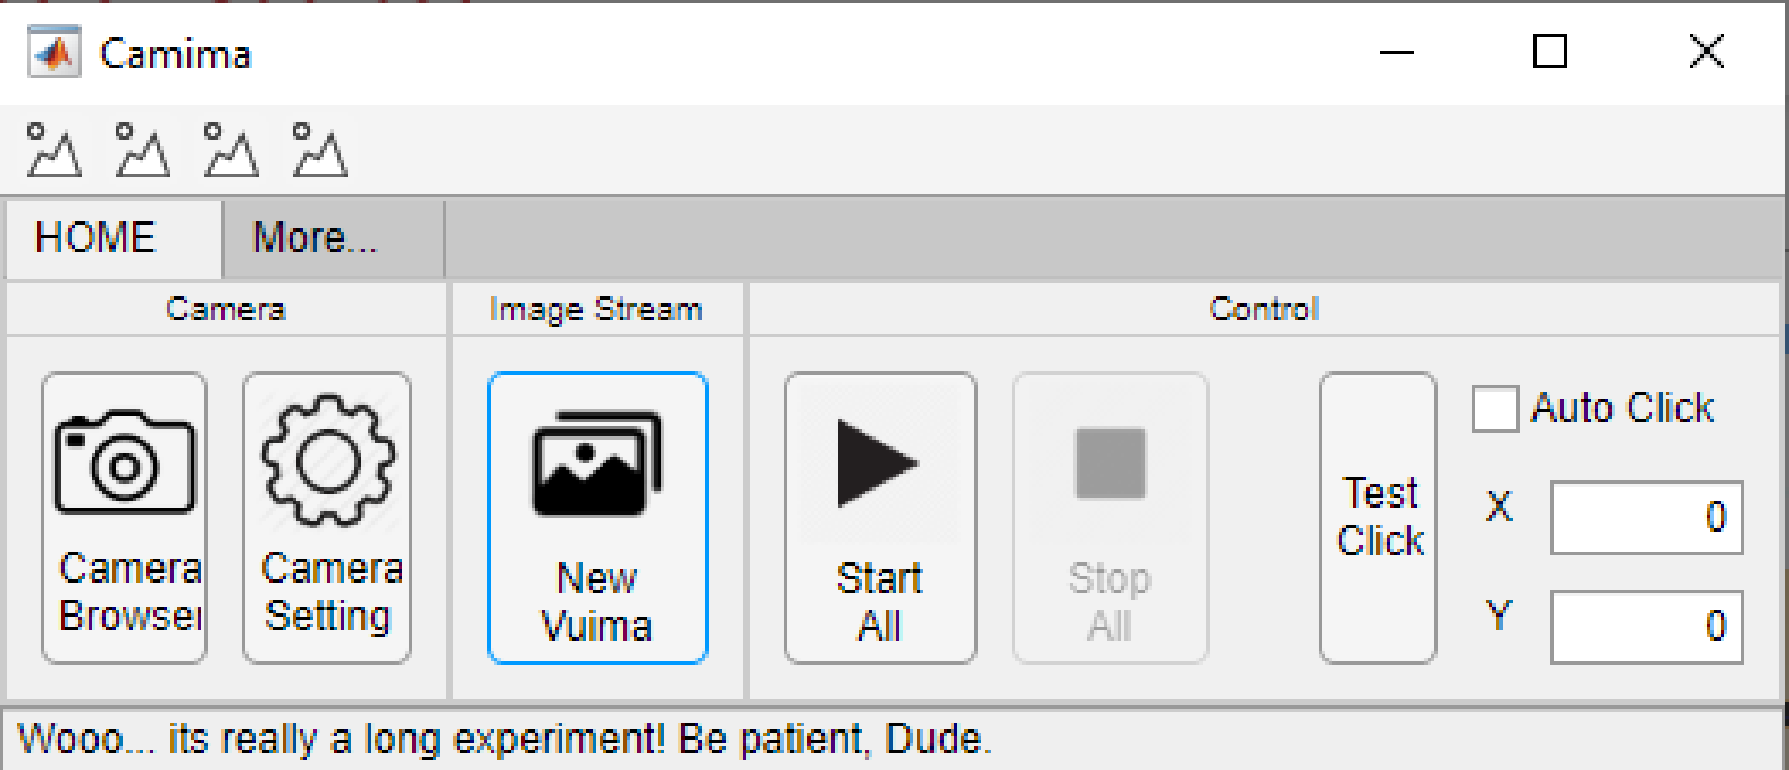
\includegraphics [width = 0.8 \linewidth]{Camima_main.pdf}
\end{center}
\caption[CAMIMA main panel]{CAMIMA Main panel.}
\label{Camima_main}
\end{figure}

% introducing the main panel (done: 2021年8月4日21:43:48)
Open the CAMIMA.mlapp in Appdesigner. Then click the Run button to run the main CAMIMA program. As shown in Fig. \ref{Camima_main}, a small panel shows you entrances for different functions:
\begin{itemize}[noitemsep,topsep=0pt]
    \item Camera Browser: Open a new panel for searching and initializing all installed cameras. (As shown in Fig. \ref{Camima_CamTree})
    \item Camera Setting: Open a new panel (CAMSET) to control each camera directly. (Fig. \ref{Camima_Camset})
    \item New VUIMA: Open an image processing panel (VUIMA) for viewing images and automatic image processing. (Fig. \ref{Camima_Vuima})
    \item Start All: For quick starting everything, including start acquisition for every camera
    \item Stop All: For quick stopping everything.
    \item Test Click: for setting a button, click after each shot with the written position on the right side.
\end{itemize}

\subsubsection{Setting cameras by CAMSET}
% camera adaptors for different venders

% add Camima_CamTree, i.e. Camera browser (done 2021-8-29 11:57:06)
\begin{figure}[htb]
\begin{center}
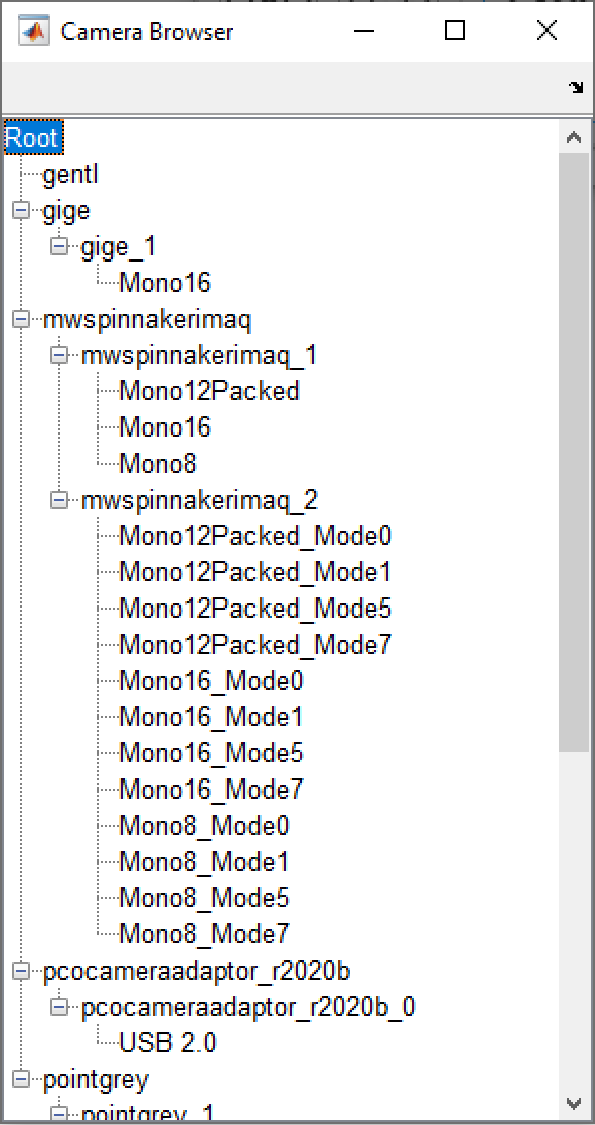
\includegraphics [width = 0.4 \linewidth]{figures/Camima_CamTree.pdf}
\end{center}
\caption[CamTree: show all available cameras for acquiring images]{CamTree shows all available cameras for acquiring images. When click the ``Camera Browser'' button in CAMIMA main panel, this tree window pops up and show you a full list of all available cameras.}
\label{Camima_CamTree}
\end{figure}

% Control the camera (2021-9-14 16:58:49)
As shown in Fig. \ref{Camima_Camset}, after catching each camera, we can control the camera manually, such as previewing, get a snap by the manual trigger and setting various parameters controlling the camera. For cameras from different vendors, the general settings are different. Thus, we generate a list in a new window, as shown in the right panel of Fig. \ref{Camima_Camset}. Users can change the private properties of the camera, such as exposure time, binning and other higher-level parameters. The ROI (Region-of-interest) can only be set when the camera is stopped as shown in the right-middle of CAMSET panel. Parameters for automatic triggering can be set in the right-bottom panel of the CAMSET window. By the way, as we mentioned before, our program can support various types of cameras which is listed as follows:

% Types of camera supported (2021-9-14 17:33:16)
\begin{itemize}[noitemsep,topsep=0pt]
    \item PointGrey USB camera
    \item BlackFly USB camera
    \item PCO USB camera
    \item camera with GIGE (web cam)
    \item other general types of camera
\end{itemize}

% add Camima_Camset, i.e. Camera setting (done 2021-8-29 11:50:03)
\begin{figure}[htb]
\begin{center}
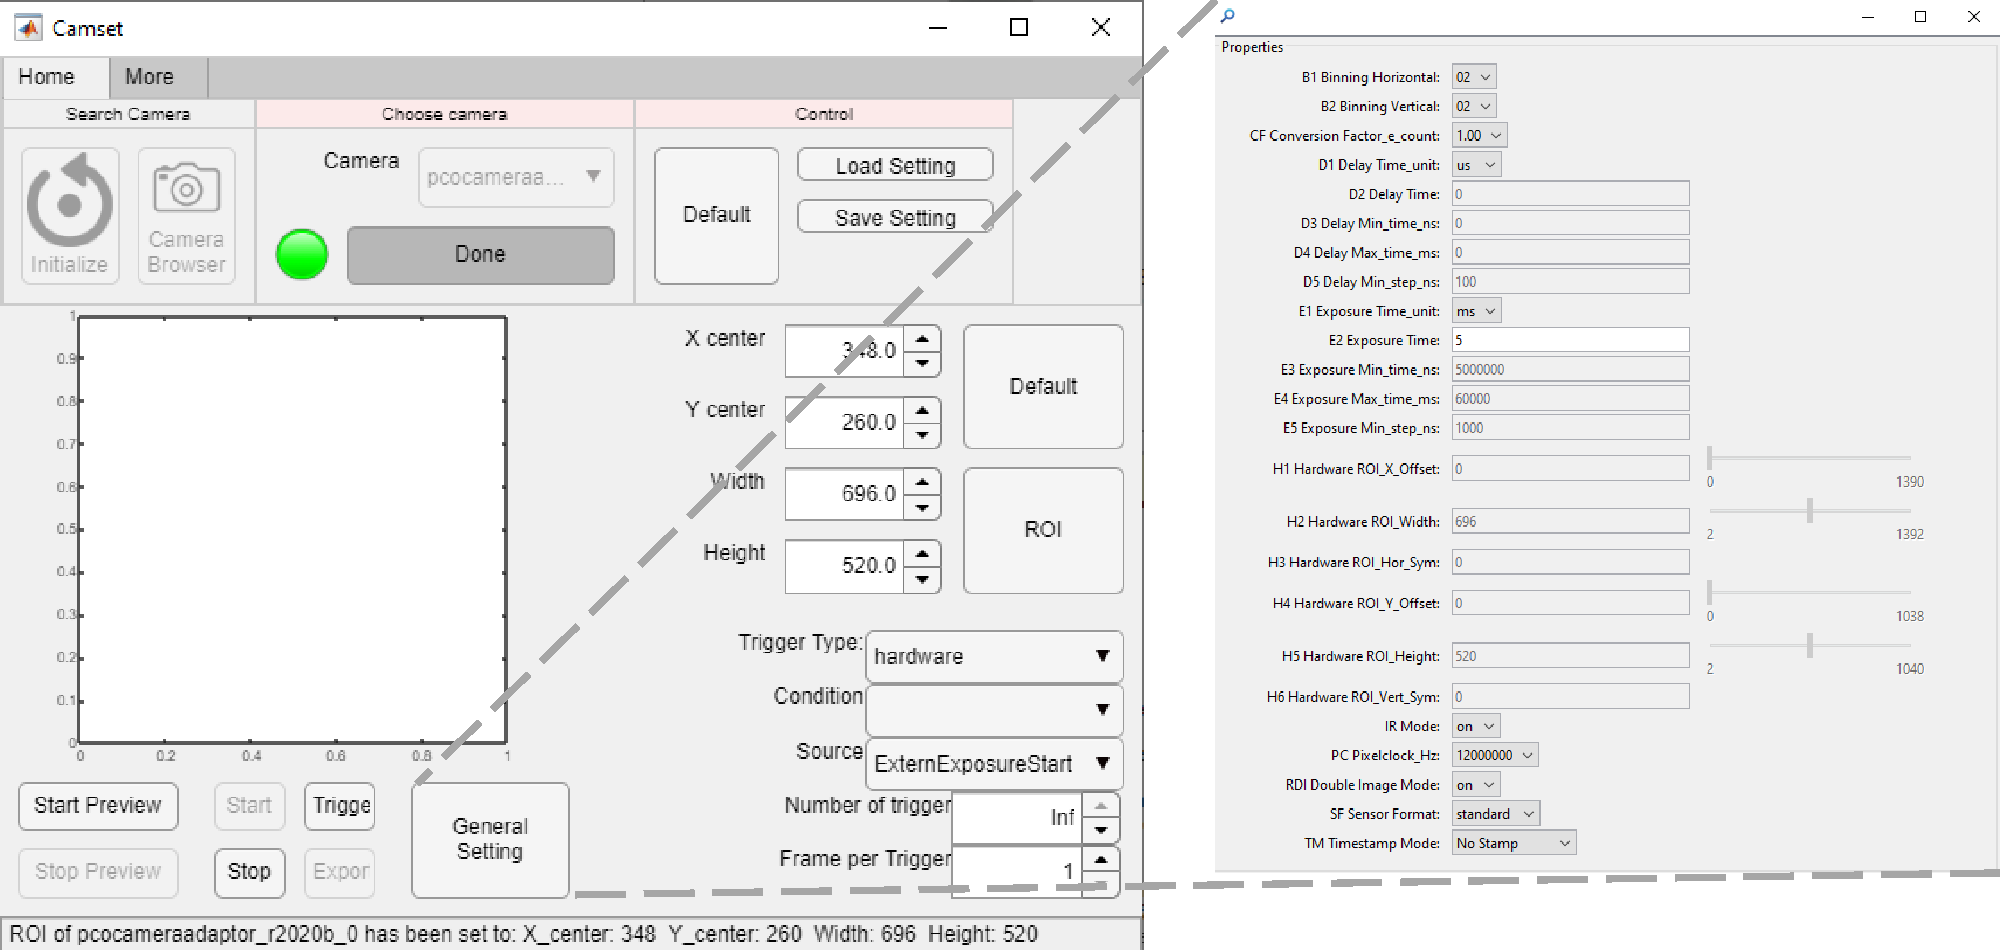
\includegraphics [width = \linewidth]{Camima_Camset.pdf}
\end{center}
\caption[CAMSET: a module of CAMIMA used to control and set cameras]{CAMSET is a module of CAMIMA used to control and set cameras. By switching the toggle, one can control multiple cameras. Besides the general setting, such as ROI and acquisition sequence, it also offers a specific entrance for each camera.}
\label{Camima_Camset}
\end{figure}

\subsubsection{Image acquisition}

% add Camima_Vuima, i.e. Viewing the image (done 2021-8-29 11:46:52)
\begin{figure}[htb]
\begin{center}
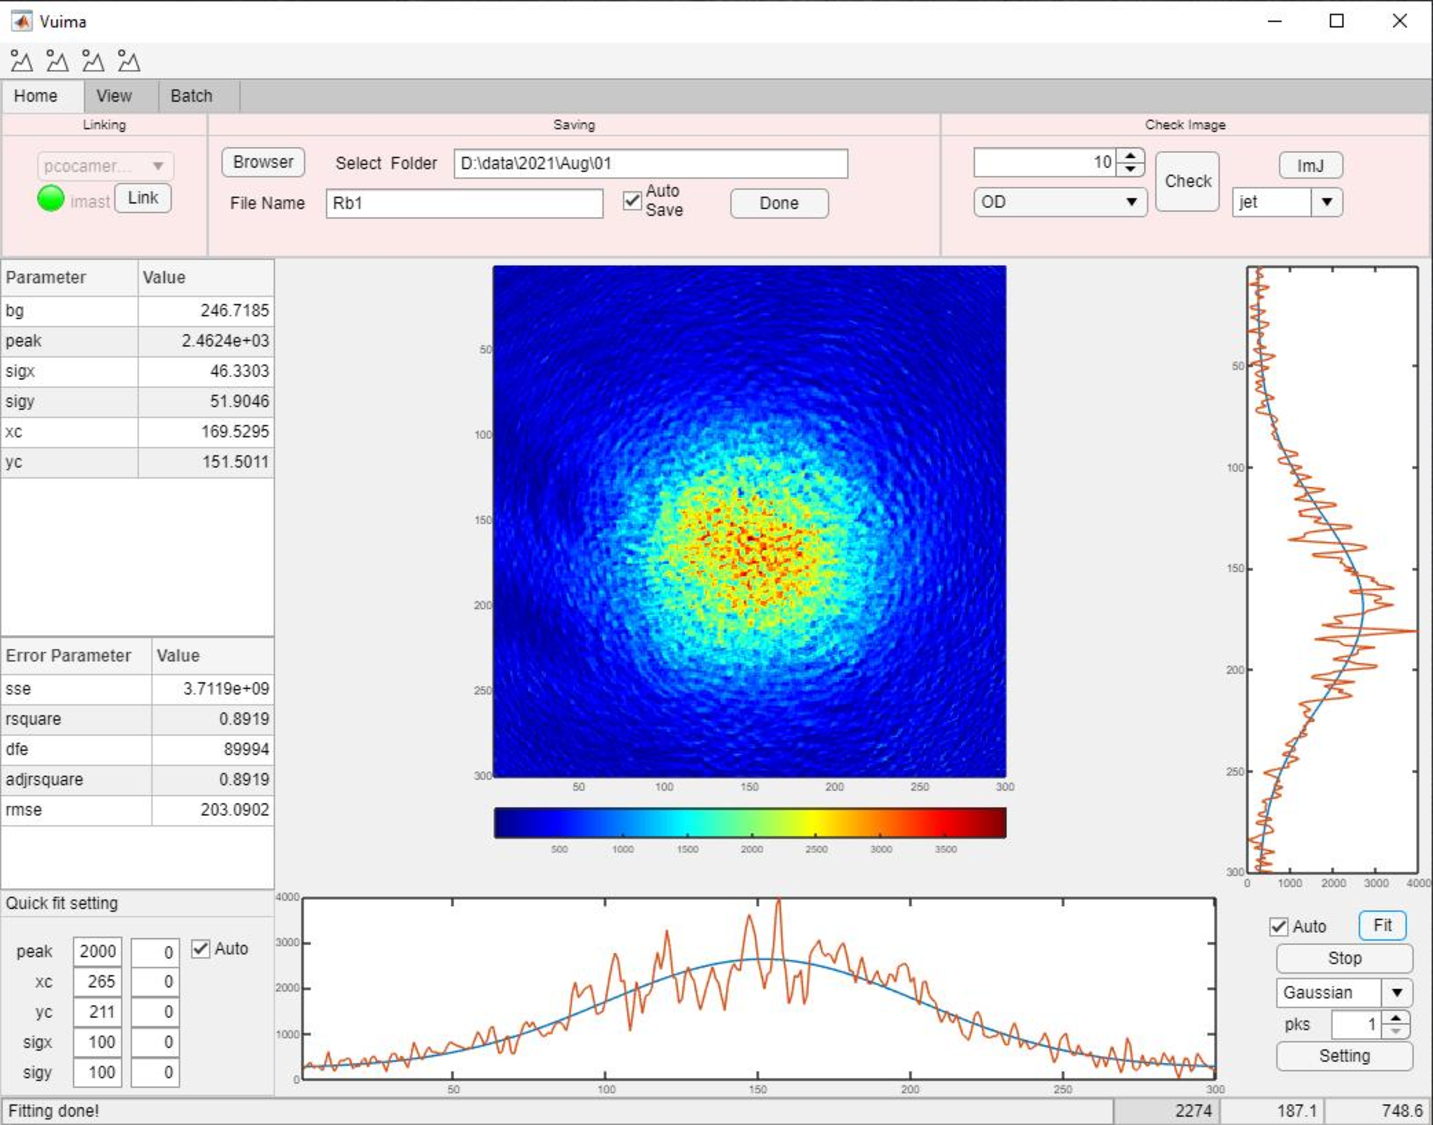
\includegraphics [width = \linewidth]{Camima_Vuima.pdf}
\end{center}
\caption[VUIMA: a module of CAMIMA used to preview image]{VUIMA is a module of CAMIMA used to preview image. The VUIMA window can be opened multiple for each image stream. Besides previewing the image, it can show the fitting results comparing to the raw data. It offers entrance for setting arbitrary fitting function.}
\label{Camima_Vuima}
\end{figure}

% time sequence of image acquisition (done 2021-9-16 20:33:38)
After configuring the camera, the platform is ready for automatic image acquisition. By setting the trigger, we can integrate the camera as part of the control system. For absorption imaging, we take three pictures for each imaging, which is achieved by setting three triggers to the camera. The picture will be temporarily cached in memory. Trigger the event by setting the number of triggers. For example, after receiving three triggers, start processing the absorption imaging picture and calculate the OD picture. For specific details of absorption imaging, please refer to that section. When we have multiple cameras that need acquisition data, each camera can complete the data collection independently.

% converting camera data to image stream (done 2021-9-16 20:38:54)
Some cameras, such as PCO, have a double image. Then, we need to divide the data collected by the camera. In order to ensure the versatility of subsequent image processing and avoid the need for different codes for different cameras, we use an adaptor to convert the raw data from cameras to independent image streams. The settings of the camera and the acquisition of the camera are in the \textit{camera stream}. Then it generates image streams. For example, a single imaging camera only provides one image stream, while a PCO double-image camera can provide two image streams. Select a specific image stream to do subsequent processing. In this way, we can say that a specific image stream is displayed in a window, i.e. VUIMA.

% show and pre-process of images on VUIMA (done 2021-9-16 21:02:31)
One VUIMA is connected to one image stream. Users can select the existing image stream in the link in the upper left corner of the VUIMA panel. As the collected images are generated, VUIMA is responsible for pre-processing the images. The statistical data will be given in the lower right corner, including the number of photons in pure light photos, by setting the exposure time, calculating the light intensity, and giving a preliminary count. For the three images collected, the data needs to be cleaned first. VUIMA first removes abnormal points and take average around them. Then it processes the OD images. Because the Log function is used, in order to avoid too many abnormal values, we adopt the cut-Log method to treat points with OD smaller than -0.2 as 0. This works for most pictures and can detect abnormal cases when sometimes the trigger is broken. For some pictures with a low signal-to-noise ratio, this limit can be modified to a lower value to ensure the authenticity of the data. Subsequently, the processed OD picture will be displayed in the middlebox, and fitting will be carried out simultaneously. The fitting result displays on the right and bottom of Vuima, in the form of slices along with the raw data points. The specific fitting will be introduced in the next section.

\subsubsection{post processing of image}

% add Camima_Fitset, i.e. Setting the fitting (done 2021-8-29 11:54:52)
\begin{figure}[htbp]
\begin{center}
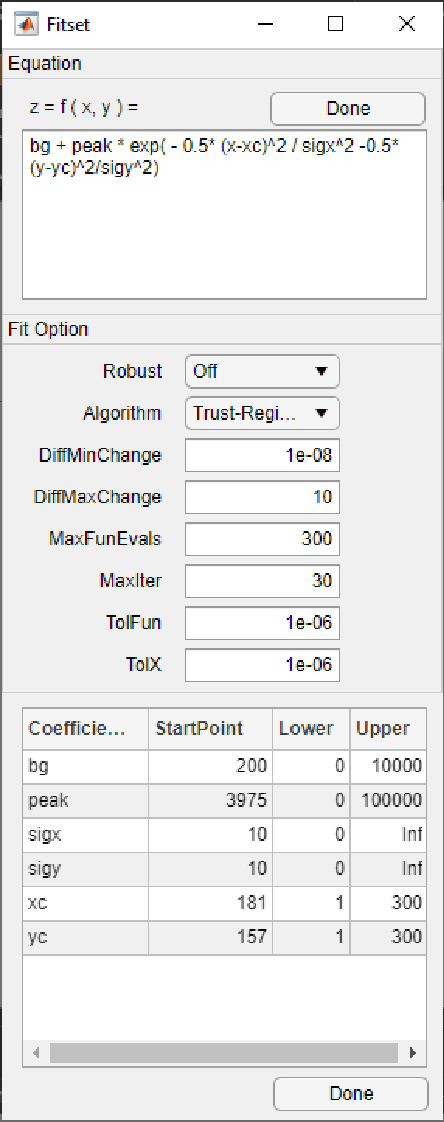
\includegraphics [width = 0.4\linewidth]{Camima_Fitset.pdf}
\end{center}
\caption[FITSET: a module of CAMIMA used to set arbitrary fitting function]{FITSET is a module of CAMIMA used to set arbitrary fitting function. Besides the default fitting functions written under the toggle button, this module offers function for easily generate arbitrary fitting function.}
\label{Camima_Fitset}
\end{figure}

% fitting of image (done 2021-9-16 21:18:21)
We first perform preliminary fitting on the collected pictures. The fitting function can be selected in the panel in the lower right corner of VUIMA. Thermal sample adopts 2D-Gaussian, BEC adopts parabola and so on. Multiple peaks can be selected. For mixed samples, one can choose a mixed model. At the same time, a user-defined module can be opened in the FITSET window. The general fitting takes typical 3-10 seconds, which can ensure that the analysis result can be obtained immediately and the decision can be made within a shot. Of course, Users can try to increase this speed. For the peak model, whether single-peak or multi-peak, one can manually select the initial value or automatically select the initial value. You can see the initial value selection in the lower-left corner of the Vuima panel. As the peak increases, more blanks can be added. The fitting result will also be stored in a CSV file for real-time import to the origin to give further analysis, such as temperature, number, density, and other parameters. At the same time, it is very convenient to compare multiple shots, draw pictures, etc.

% statistic data from image (done 2021-9-16 21:26:40)
The fitting data is first displayed in the table on the left. Users can get fitting errors by sliding the form to the left. In addition, indicators such as r-square value are given in the middle on the left. Adj-square is used to indicate which model is better to use when the model is not clear. In order to facilitate the data analysis after the experiment, Vuima has developed a batch processing module for batch processing of a large number of pictures. Because of the convenience of programming, this function has a high degree of freedom, and users can freely add the codes they want to process in the module.


\subsection{Vision and outlooks}

% Vision (done 2021-9-16 21:31:37)
From the perspective of experimental physics, there are two primary purposes for using or developing new technologies: The first is to detect physical quantities that were previously undetectable through technological advancement. The second is to improve the efficiency of experiments and work through technological advancement. The former makes the frontiers of experimental physics one step forward, while the latter can make experiments one step further away from industrialization. Cold atom physics has been developed for more than two decades. Nowadays, with the rise of quantum computing, it is time to consider further substituting industrialization methods into experimental research to pave the way for research-industry transformation.

% Purpose of developing the program (done 2021-9-16 21:35:49)
Strictly speaking, CAMIMA is only the second half of the entire cold atom experiment timing system, which is the data acquisition part. A complete experiment sequence system should be able to record all the data of each experiment: including sequence setting parameters, checking and testing parameters. Generally, we will focus the laboratory data on only what we want to control, such as a specific frequency or power, and what we want to see, such as absorption imaging pictures. However, all measured quantities are part of the experiment. A complete record has two advantages: First, a complete record includes complete monitoring, which can avoid out-of-control conditions. Second, a complete record can make the data of each shot more valuable. For example, the data collected on different days is comparable. Through systematic data analysis, there will be unpredictable discoveries. Furthermore, these are inseparable from introducing new, efficient data acquisition technology and data analysis and processing technology. In general, martial arts in the world can only be broken quickly. The pursuit of efficiency is the eternal theme of science and research.

\section{Fast magnetic field control}
\label{sec:fastcoil}

% why we need fast-magnetic control (done 2021-9-16 22:33:50)
As we mentioned in the section about Feshbach resonance, by tuning the magnetic field, we can easily control the scattering properties of atoms, i.e. the interaction strength. In the previous set-up, we use a large Helmholtz coil with 70 turns. The coil's inductance is three mH, which is huge, introducing a significant time constant. So, even using a driver with 100V(check), we will have a rising slope of about 1 ms, which is not fast enough for our requirement to control the interaction. Our request depends on the time scale of the research object. For example, a typical BEC with a scattering length of 100 $a_0$ order will have a time scale of less than 1 ms. Thus, we need a new magnetic field control system with the time scale of $\mu$s level to control the interaction fast. Then we can make sure the sample's size of other parameters changing much slower than the interaction changes.

% fast coil design (done 2021-9-23 11:59:31)
\begin{figure}[htb]
\begin{center}
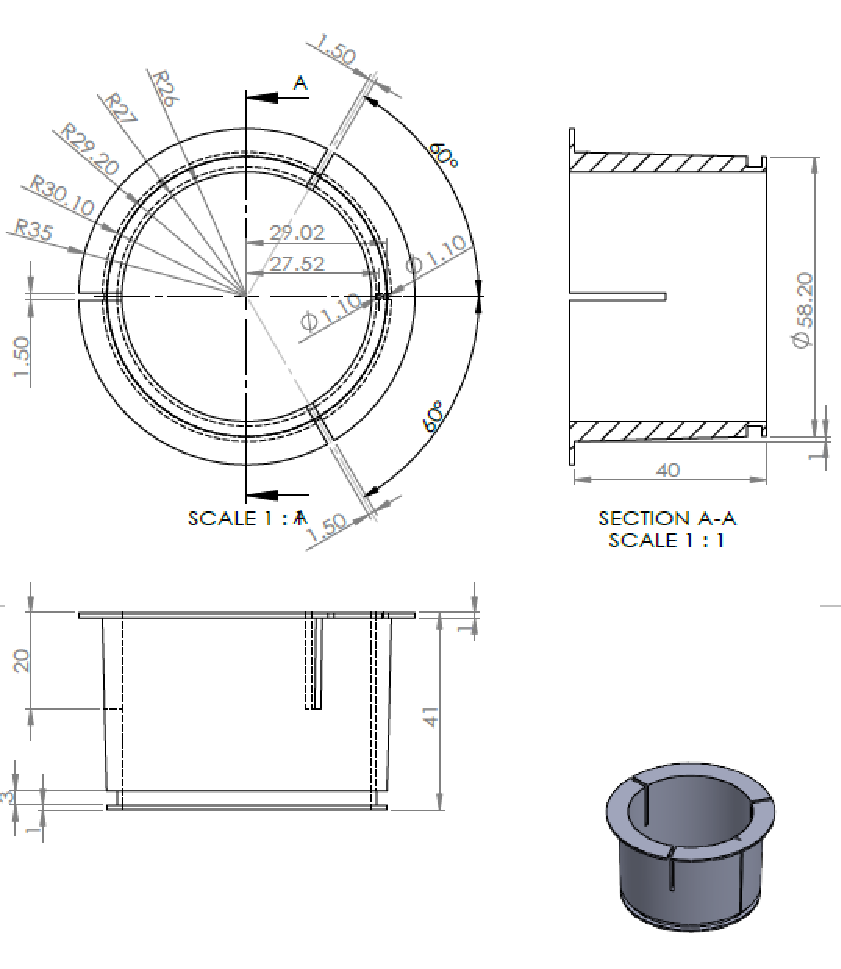
\includegraphics [width = 0.6\linewidth]{Apparatus_coil_holder.pdf}
\end{center}
\caption[Fast coil holder]{Fast coil holder for adapted to existing main coil system.}
\label{Apparatus_coil_holder}
\end{figure}

% What is fast coil and how to build one. (done 2021-9-16 22:41:19)
So, with the above request, we need to build another coil that can generate a small but fast magnetic field. The limitation is the coil's inductance, so we reduce its turns to as few as possible. However, with fewer tunes, the magnetic field can generate a less magnetic field. So we need to make a trade-off here. Finally, we choose a diameter 60 mm coil pair with six turns for each one. Also, to generate a larger magnetic field, we put it as close as possible to the cell. The set-up with the main Feshbach coil is shown in Fig. \ref{Apparatus_coils}. To adapt our previous large coil, we designed a holder made of polyvinyl as shown in \ref{Apparatus_coil_holder}. Moreover, the holder winding with the fast coil is inserted into the 2-inch optical path to avoid blocking the MOT beam.

% current driver and its test data (done 2021-9-17 10:21:11)
To drive this fast coil, we need a current driver that fast turns on/off and makes a precision control of the current with tiny leaking current. So, with Lintao's help, we design a fast coil driver with two groups of JFET. Each group is several JFETs set in cascade. This design uses the intrinsic fast-changing property of JFET compared to MOSFET, which typically possesses large junction capacitance. Also, cascade sets of JFETs can reduce the leak current from the base since after several levels the current in the base can be reduced to $\mu$A level or even better. The driver schematic and simulation by Tina-TI can be found in the appendix. \ref{chap:M&E}.

% fast coil couple with main coil and environment (done 2021-9-23 12:02:43)
\begin{figure}[htbp]
\begin{center}
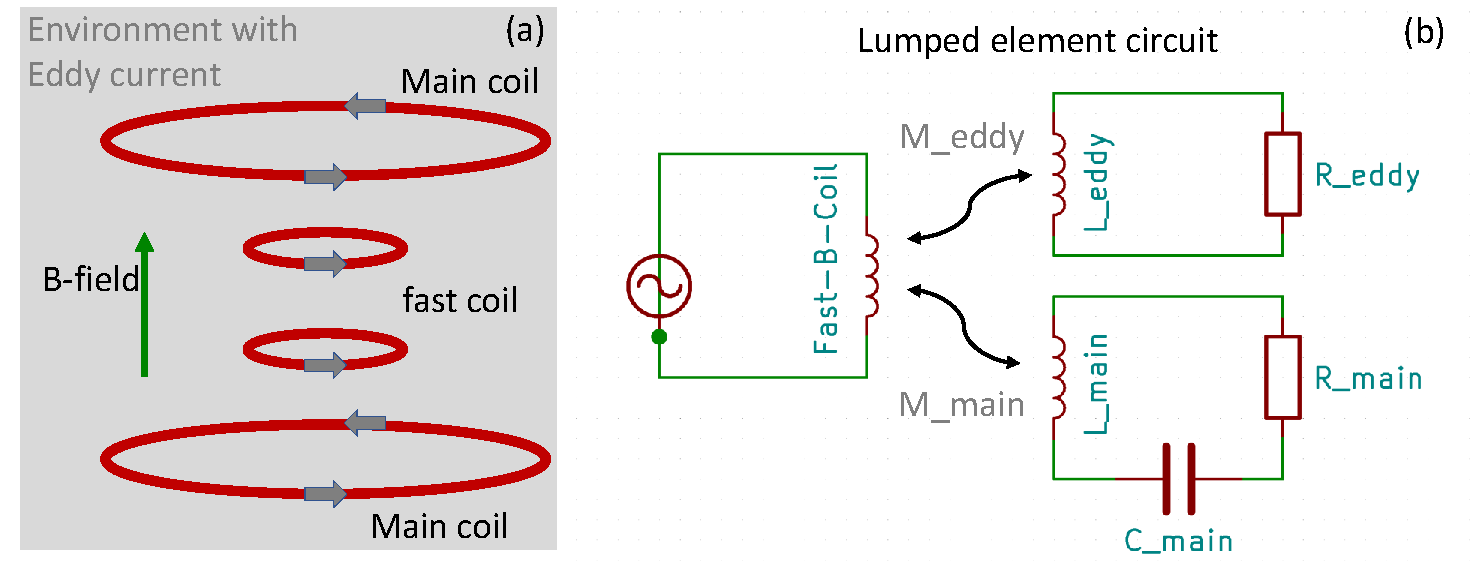
\includegraphics [width = \linewidth]{Apparatus_coils.pdf}
\end{center}
\caption[Fast coil, main coil and environment]{(a) set-up with main coil for generating hundred-Gauss level magnetic field and fast coil can change magnetic field in $\mu$s time scale. There is also the coupling between these coils and environment, such as metal optical board around the coil or cables for connecting antennas. (b) Lump circuit for simulating the system with two coils and the environment.}
\label{Apparatus_coils}
\end{figure}

% design of fast coil (done 2021-9-21 21:55:54)
Two parts of the fast coil are put as close as possible to avoid introducing more curvature since the cell is too large for the Helmholtz condition. Finally, the fast coils are separated 70 mm with a diameter of 60 mm. Each coil has an inductance of less than 5 $\mu$H. This enables us to generate a magnetic with a slew rate larger than 500 G/ms. In other words, we can change the magnetic field with several $\mu$s when working around the Feshbach resonance. As shown in Table. \ref{tab:coils}, by injecting 1 A, we can get 0.67 G (set in Helmholtz type). Our current controller can bear a surge current of less than 10 A as we use two TIP31. So, finally, we can get a maximum magnetic field of 6.7 G which is definitely enough as a fast trim in daily experiments.


% add table here about fast coil and main coil (done 2021-9-21 21:56:05)
\begin{table}[htbp]
\centering
\begin{tabular}{|l|l|l|}
\hline
                        & Main coil      & Fast coil             \\ \hline
Coil sepa. to atom (mm) & 25 – 85        & 35                    \\ \hline
Coil radius (mm)        & 52 – 90        & 30                    \\ \hline
Coil inductance         & $\sim$3 mH     & $\sim$5 $\mu$H        \\ \hline
Magnetic field per A    & $\sim$8.2 G    & $\sim$0.67 G          \\ \hline
Ramp speed              & $\sim$0.6 G/ms & \textgreater{}500 G/ms\\ \hline
Number of turns         & 70             & 6                     \\ \hline
\end{tabular}
\caption[Parameter table of main coil and fast coil]{Parameter table of main coil and fast coil}
\label{tab:coils}
\end{table}

% coupling of fast coil and main coil (done 2021-10-28 17:19:01)
As explained in \cite{cumby2012exploring}, we need to consider the coupling of the fast coil, the main coil and the environment. Since, these coupling will cause oscillation and jiggle when quenching the current in the fast coil. As modeled by the lump elements, as shown in Fig. \ref{Apparatus_coils}. The Fast coil are simulated as a inductance driven by a current source. fast coil has mutual inductance with main coil and the environment. The main coil is viewed a RLC circuit and the environment only as a RL circuit. With this lump circuit simulation, we can qualitatively figure out however these three things coupled to each other. However, more detailed parameter can only be achieved by measure the response of the system. By adding a quenching signal, we can get the response of the whole system. Then, we can do feed-forward to compensate the overshooting or jiggles since the speed of fast coil is about 1000 times faster than the Main coil and the environment.

% Why we need dynamic compensation
There are two reasons for us to do the dynamic compensations, first is the coupling of the fast coil and main coil, and the environment will cause a jigger when we quench the current of the fast coil. To avoid this jigger, we feed-forward set the current to compensate for this overshooting. The second is for the droplet experiment: because the magnetic field generated by the main Feshbach coil has a gradient, when we do ToF, the magnetic field at atom position changes with time. So, to keep the magnetic field on atoms unchanged with ToF, we need this dynamic compensation. For the first case, the compensation needs very fast, so we use the fast coil. For the second one, it is a relatively slow-changing process. So we only use the shim coil to do the compensation. 

\section{Other Technical Issues}
\subsection{Magnetic field gradient compensation}
\label{subsec:gradientcompen}

%Why we need to compensate the B-field gradient (done 2021-9-24 17:34:04)
As mentioned before, we use a pair of Feshbach coils to generate a large bias magnetic field to control the Feshbach resonance. However,  the imperfection of the coil, such as asymmetry of coils and imperfection of distance between up-down Helmholtz coils, renders a gradient and curvature of the magnetic field. This effect can be easily detected by the free-falling of atoms in the high magnetic field. If one finds that the atom's acceleration deviates from gravity acceleration, there must be a gradient. Another evidence is the MW (RF) spectroscopy for an elongated sample that could detect the horizontal gradient. When we free-falling Rb or Na under a high magnetic field, if the acceleration becomes different from gravity, we can use it as an indicator of magnetic field gradient.

% What is our gradient looks like? (done 2021-9-17 22:37:43)
Before talking about cancelling this gradient, we first measure it. The method is simple, following the MW transition calibration method, we apply the MW pulse coupling the $\ket{1,-1}$ and $\ket{2,0}$ state. To get the spatial distribution of the magnetic field, we first let the atom free-fall, then apply the MW pulse at different ToF. Even though the gradient affects the atom's position by adding an extra acceleration, considering the small effect related to gravity, this can be neglected. Not only exists the gradient but also the the curvature of the magnetic field because the spatial changing B-field is definitely more than linear. By a simple quadratic curve fitting, we get the curvature of about $2.47 \times 10^3$ G/cm$^2$ and an average gradient of about xx G/cm. One thing that needs to be noticed here is that we measured only the magnetic field gradient in the vertical direction, which is our main contribution. As we can see in the horizontal direction, the acceleration is even much lower than that in the vertical direction, which infer that this gradient should come mainly from the wrong distance of the Helmholtz coil.

% gradient compensation method
\begin{figure}[htb]
\begin{center}
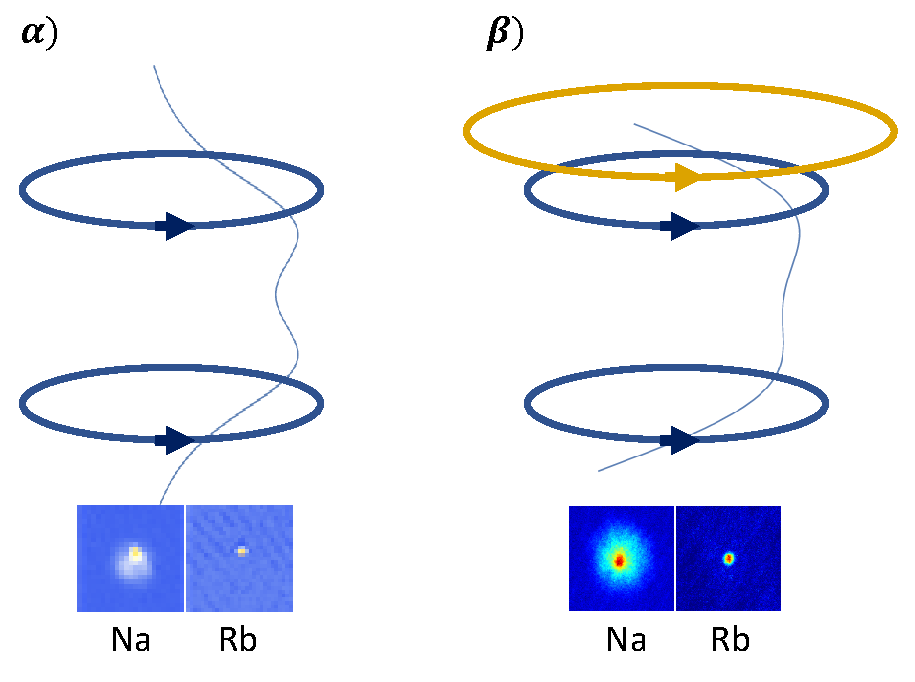
\includegraphics [width = 0.7 \linewidth]{Apparatus_gradient-compen.pdf}
\end{center}
\caption[Method of compensating the magnetic field gradient]{$\alpha$) B-field curvature and gradient affects free falling of atoms. $\beta$) Using only UP shim coil to compensate gradient.}
\label{Apparatus_gradient-compen}
\end{figure}

% How to compensate the gradient and curvature (done 2021-9-17 23:42:44)
It is hard to totally compensate the curvature because it will need to entirely recover the Helmholtz condition, which requires a much larger magnetic field to be added to the existing system. So, to solve the problem we meet, we degenerate to compensate the average gradient to zero inside the interesting ToF we care. So, we can add another magnetic gradient in the vertical direction and adjust its current to find the best compensation point. We use one of the up-down shim coil (e.g. up coil) as a preliminary test. As shown in Fig. \ref{Apparatus_gradient-compen}, we can generate an inverse direction gradient opposite to the main coil. 

% add find compensation point method (done 2021-10-28 18:17:22)
\begin{figure}[htb]
\begin{center}
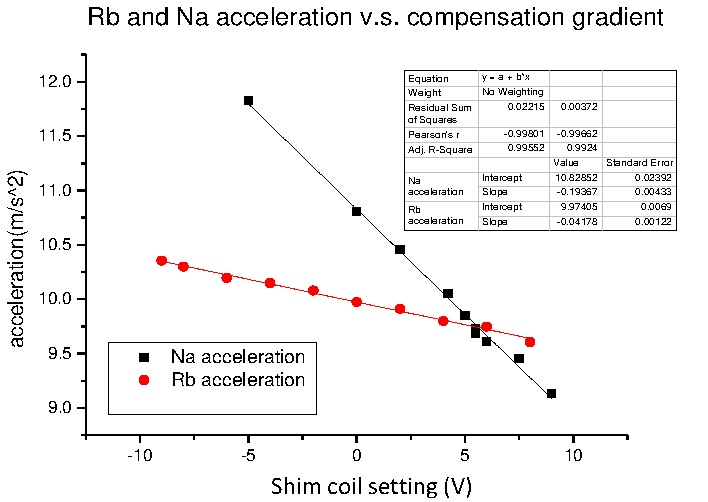
\includegraphics [width = 0.7  \linewidth]{Apparatus_compen_method.pdf}
\end{center}
\caption[Method of searching the compensation point]{By searching the cross point of Na and Rb sharing the same acceleration, we find the compensation point.}
\label{Apparatus_compen_method}
\end{figure}

% find the best compensation point (done 2021-9-17 23:54:51)
We change the current of the shim coil and test the acceleration of the atom to find the compensation point. As the dipole moment of Na and Rb is quite different, we can also find the intersect point of them, which represents zero average gradient compensation point, as shown in Fig. \ref{Apparatus_compen_method}. Finally, we tune the shim coil to the current at the intersection. We measure the magnetic field with the MW spectroscopy method and compare the result with the previous non-compensation one, as shown in Fig. \ref{Apparatus_mag_before_after}. It is evident that the mean gradient is reduced significantly; however, the curvature is still there. The compensated gradient on average (we take the 10 ms ToF as an average position) are about 0.11 G/cm, which should be enough to observe BEC mixture free-falling.

% before and after compensation measurement
\begin{figure}[htb]
\begin{center}
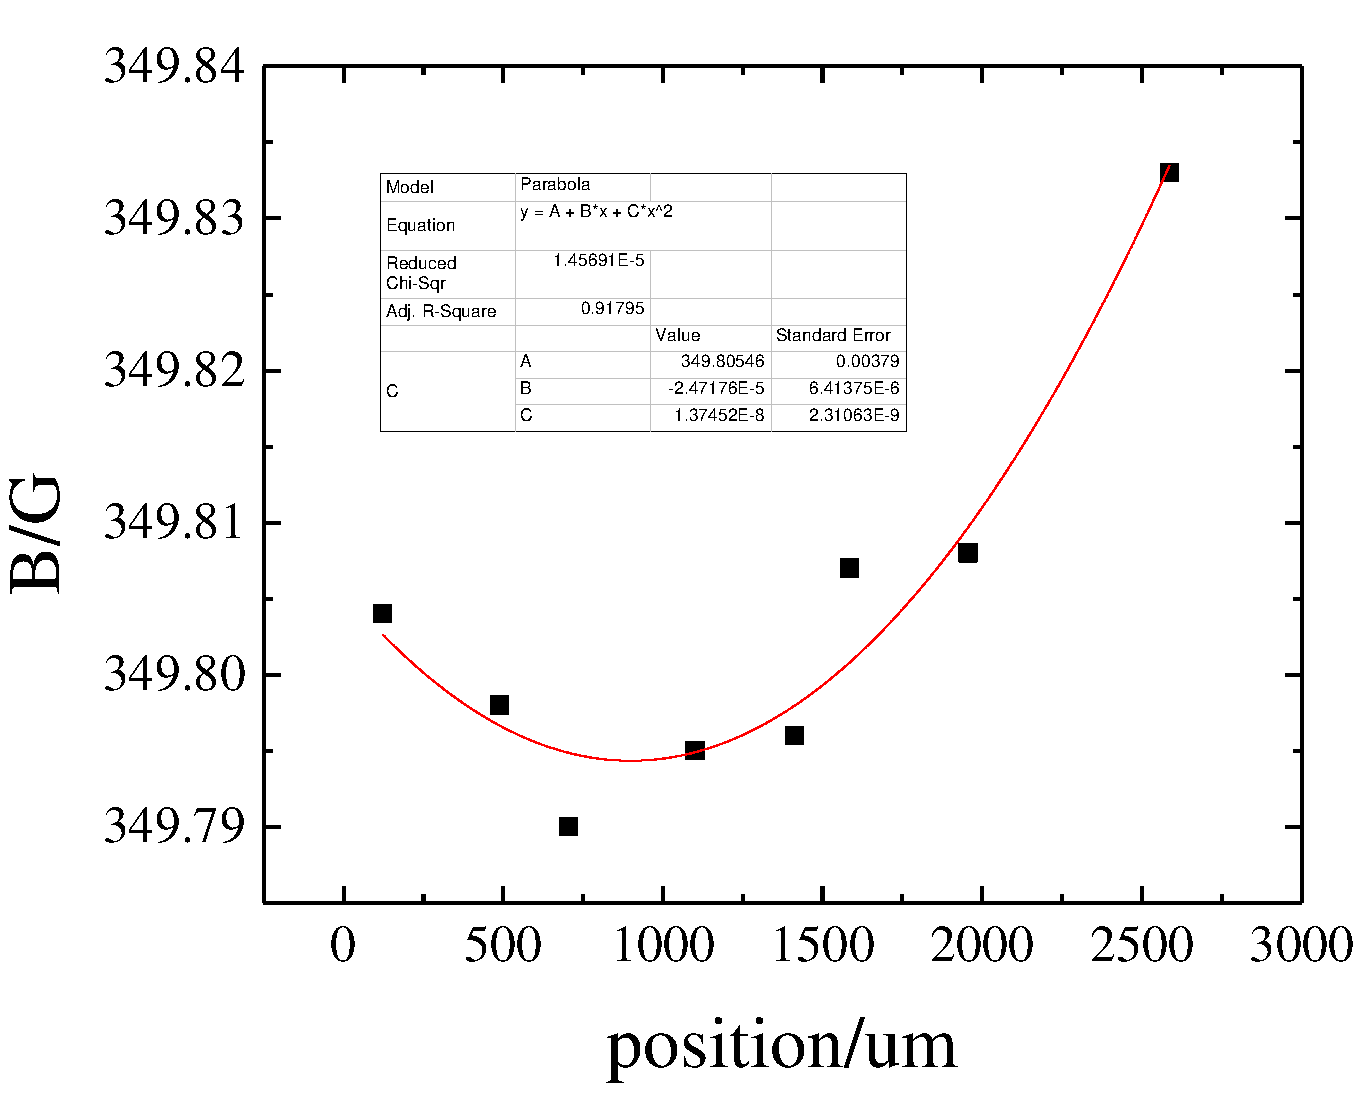
\includegraphics [width = 0.7 \linewidth]{Apparatus_mag_before_after.pdf}
\end{center}
\caption[Magnetic field spatial distribution at vertical direction after compensation]{Shows the magnetic field spatial distribution at vertical direction after compensation. It still remains gradient and curvature, however much smaller than the one before compensation. We fit it with a quadratic function to get the local gradient and curvature for compensation later.}
\label{Apparatus_mag_before_after}
\end{figure}

\subsection{Microwave full-wave loop antenna}
\label{subsec:FWLA}

% Why we need to build the 2.57GHz and 7.5GHz full-wave loop antenna (done 2021-9-22 00:15:26)
As described in SubSec. \ref{subsec:high_mag_absop_image}, the internal states of atoms can be controlled by the electromagnetic wave. Typically, to drive transition between two different hyperfine states, we need to use micro-wave(MW), which has a wavelength of about 0.3 m to 3 m, i.e. 300MHz to 300 GHz for frequency in the vacuum. The hyperfine splittings for Na and Rb atoms are 1.7 GHz and 6.8 GHz at zero magnetic fields. When the magnetic field increasing to 350 G (since we typically use the 347 G Feshbach resonance to control the inter-species interaction), the splitting between $\ket{F=1,m_F=1}$ and $\ket{F=2, m_F=2}$ states are 2.6 GHz and 7.5 GHz for Na and Rb separately. Thus, we need an antenna that can work well at this frequency. Here, ``work well'' commonly has two meanings: First, the antenna's standing wave ratio (SWR) is approaching 1, which means it can transmit most power to coil instead of reflecting it back to the power amplifier. Secondly, we need the atom to feel the largest amplitude of E-field because the transitions between different F-state is mainly connected by electron dipole, i.e. an electrical dipole transition. (here, need more carefully check) So, the antenna's position, including its distance to the atom and its direction angle, is critical to maximizing the utility of the antenna. We can define the efficiency for the above two processes as $\mu_{trans}$ and $\mu_{anta}$, and the total efficiency is just their multiplication.

% talk about near-field and far-field difference (done 2021-9-22 00:21:18)
A commercial antenna is typically designed to work well in the far-field region. The radiation power declines inversely proportional to the distance. Thus, to increase the power on the atom, we put the antenna to the atom as close as possible. However, this renders the radiation on the atom turns to be near-field instead of far-field. As depicted in Fig. \ref{antenna_EM}, the electric and magnetic field line of a dipole antenna is plotted as blue and red separately. At a considerable distance of the antenna, the electric field line is almost perpendicular to the \(\hat{r}\) direction. However, when getting closed, it shows more portions to the \(\hat{\theta}\) direction. This tells us that the near-field electromagnetic field of the antenna behaves quite different from its far-field one. Both electric and magnetic field lines are perpendicular to the Poynting vector in the far-field region, which shows its radiation properties. However, the near-field cannot be treated as radiation; instead, we typically treat it as a ``quasi-stati'' field. A quasi-static field means the distribution of EM field is the same as it in electrostatics, except an oscillation in magnitude with \(e^{i\omega t}\). In engineering, these study is essential to wireless-charging, proximity sensors and so on.

% near-field and far field EM field of antenna (done 2021-9-22 00:26:56)
\begin{figure}[htb]
\begin{center}
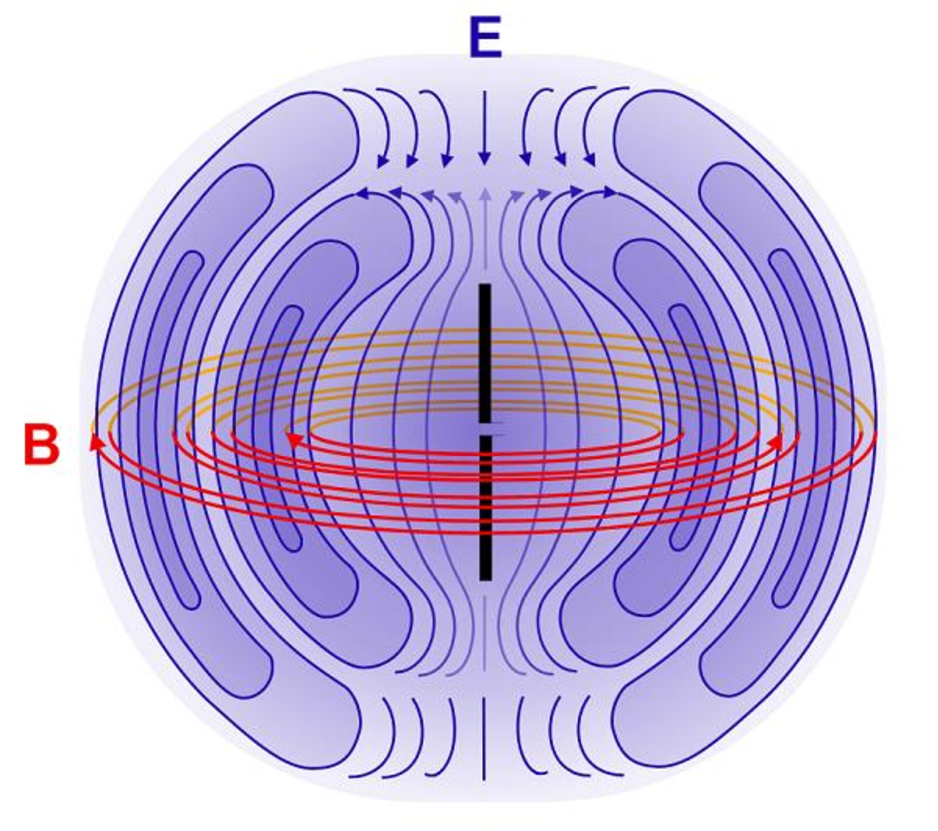
\includegraphics [width =0.5 \linewidth]{Apparatus-EM_field_antenna.pdf}
\end{center}
\caption[Electromagnetic field of a dipole antenna]{Electromagnetic field of a dipole antenna (image from \href{https://www.everythingrf.com/community/what-is-the-difference-between-a-monopole-and-dipole-antenna}{Everythingrf Website}). The near-field and far-field distribution are quite different as described in text.}  
\label{antenna_EM}
\end{figure}

% what previous one done, and what's the problem of it (done 2021-9-22 01:22:59)
Previously, we used a horn antenna for Rb MW transition at 6.8GHz. The distance between horn and atom is about 10-15 cm. The problem to put the antenna closer to the atom is its colossal size which could block the optical path, and its metallic body could disturb the strong magnetic field of a large Feshbach coil, causing a gradient on the atom. So the nearest position we can put is about 10 cm away from the atom, and the Rabi frequency of Rb $\ket{1,1}$ to $\ket{2,2}$ transition at 350 G (7.5 GHz) is less than 1 kHz with a 40 W power amplifier. The correspondents \(\pi/2\) pulse duration is about 250 $\mu$s which is too long for most of our experiments, such as high magnetic field image or too weak for dissociating the FR molecule. Thus, we need to upgrade it to enhance the Rabi frequency.

% full-loop antenna (done 2021-10-29 12:47:53)
\begin{figure}[htb]
\begin{center}
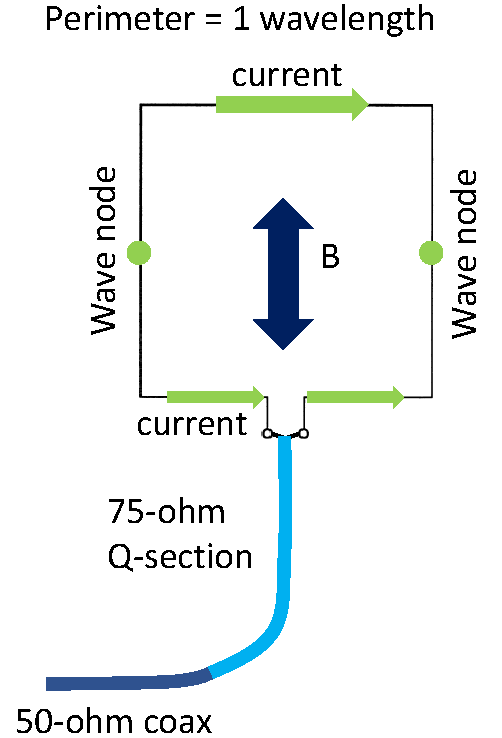
\includegraphics [width =0.5 \linewidth]{Apparatus_full_antenna.pdf}
\end{center}
\caption[Full loop antenna and Q-section for impedance matching]{Full loop antenna and Q-section for impedance matching. The parameter of the loop is set to be one wavelength of the emitting MW. The 75-ohm Q-section is for impedance matching.}  
\label{Apparatus_full_antenna}
\end{figure}

% How to improve? what is full-wave loop antenna? (done 2021-10-29 12:55:03)
So, a naive solution is to put the antenna as close to the cell as possible and try to shrink its size smaller and thinner. Therefore, the loop antenna will be a proper choice. A loop antenna is just a simple loop connected to the signal generator. However, for our case with frequencies at 2.6 GHz and 7.5 GHz, The wavelength is around several cm to tens of cm. This is comparable to our coil size, which could introduce a severe problem with impedance matching. A standard solution is making the perimeter of the loop antenna just a full wavelength, which is called the full-wave loop antenna as shown in Fig. \ref{Apparatus_full_antenna}. When the scale of the antenna is closed to wavelength, the distribution of radiation becomes quite different to those small-loop antennas. This can be explained by a simplified picture, as shown in Fig. \ref{Apparatus_full_antenna}. At the joint place, and directly opposite current changes with the largest amplitude, and there placed two nodes at the quarter wavelength place to the joint. However, the current almost has the same phase on the whole coil for a small loop antenna. Therefore, they have different radiation patterns.

% How the antenna works? (done 2021-10-29 13:00:50)
According to the near-field quasi-static EM field theory, the maximum radiation appears at \(\lambda/4\) away from the coil plane. Furthermore, the power at the centre of the coil is zero, which is different from the case of a small-loop coil. For our case with $f=2.6$GHz, the wavelength is about 12 cm. So, we place the coil 3 cm away from the atom to achieve the largest power. For the 7.5 GHz case for Rb MW in a high magnetic field, we set the perimeter of the loop to 4 cm. However, we cannot put the coil 1 cm away from the atom due to the distance limitation. Finally, by making the trade-off between the optical paths and MW power, we set the tiny coil at the side of the cell with a 45-degree angle and distance to atom about 3 cm. 

% Set-up and impedance matching (done 2021-9-22 02:35:26)
After preparing the coil, we set up the standard MW power amplifier circuit for it. Before the amplifier, we add a switch controlled by a TTL signal, and the signal generator is an SG-386. The critical point to increase the efficiency from power amplifier to the coil, i.e. \(\eta_{trans}\), we need carefully consider the impedance matching from the transmission wire to the loop coil. As shown in Fig. \ref{Apparatus_full_impedance}, we demonstrate several full-wave loop antennas with different shapes. They have different impedance; the ideal one is rectangular with an aspect ratio of 1:2, with 50 Ohm impedance. However, for our case with a round shape, we have the coil with 133 Ohm. Our transmission line and power amplifier are all 50 Ohm, so we need to match impedance. We use a balloon, i.e. a 75 Ohm transition line, to enhance the transmission rate. As shown in Fig. \ref{Apparatus_full_antenna}, the signal can be reflected at the boundary of two lines with different impedance. Boundaries of 50-to-75 and 75-to-133 offer two reflection waves. If we choose a proper length of the 75 Ohm line, we can cancel the reflection thanks to their superposition. 

% different shape and impedance (done 2021-10-29 13:12:09)
\begin{figure}[htb]
\begin{center}
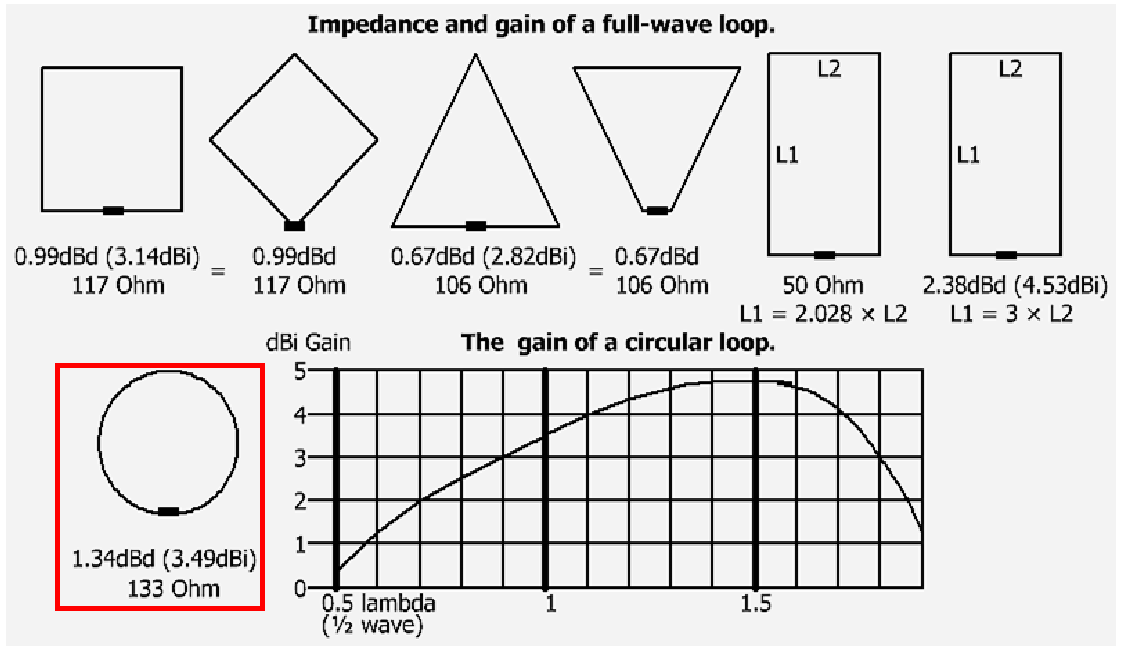
\includegraphics [width =0.8 \linewidth]{Apparatus_full_impedance.pdf}
\end{center}
\caption[Impedance of full-wave loop antenna with different shapes]{(image from \href{https://pa0fri.home.xs4all.nl/Ant/Quad/quadeng.htm}{pa0fri.home}) Impedance of full-wave loop antenna with different shapes. In our experiment, we use the round-shape to matching the optical path of MOT beam. In experiment in LH24C, the 1:2 rectangular is better since there is no need to do the impedance matching.}  
\label{Apparatus_full_impedance}
\end{figure}

% Test of the coil (done 2021-9-22 02:43:53)
Even though we know how long the q-section line should be, we still need to do the offline test for its performance because the length of several cm is too short to allow uncertainties from the imperfection of the coil's shape and impedance. These incomplete can cause the phase of reflection wave shifting and decline the effect of impedance matching. Therefore, we build a series of coils with different lengths of its q-section and measure its return loss rate by a directional coupler. As shown in Fig. \ref{SWR_measure_method}, we send the signal into the output port of a coupler, and the reflecting wave from the antenna (connecting on the input port of the coupler) will be coupled a small portion into the coupled port and detected by an analyser spectrum. By calculating the reflecting power and injection power, we plot the return loss rate as a function of the length of the q-section line in Fig. \ref{antenna_return_loss}. We find the period does coincident with the half of wavelength. There is a shift that could be attributed to the imperfection of the q-section line. By fitting with a sine function, we extract the period, shift and so on. Finally, We can now build the coil with the lowest return loss for covering our usage frequency.

% test the SWR by directional coupler (done 2021-10-29 13:06:48)
\begin{figure}[htb]
\begin{center}
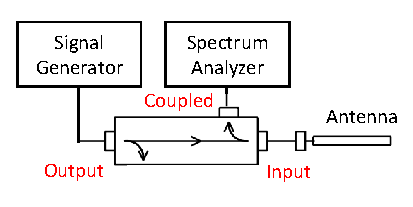
\includegraphics [width =0.7 \linewidth]{Apparatus-measure_SWR.pdf}
\end{center}
\caption[Test method of the return loss of the antenna]{Test the return loss of the antenna by a directional coupler. Noticed that the input signal is sent from the Output port of the coupler.}
\label{SWR_measure_method}
\end{figure}

% Online test (need more modification)
Finally, we put the coil onto the atom cell. First, we test the transmission rate of the coil online to make sure the impedance matching works well since the offline test with an environment open; however; however, the online environment is full of different metals around the coil, which could change the boundary condition and shift the impedance of the coil. So, we use the same method to test the transmission rate of the coil, as shown in Figure. The bandwidth is about xxx MHz. Then, we test the Atomic Rabi frequency to measure the final performance of the coil. We apply the MW pulse for Na at 350 G and get the Rabi frequency at different freq or detuning?. As shown in Figure, we test the saturation power and get a Rabi maximum of about 100kHz(check the number). This could allow us to make a pi pulse within 10 us which is enough for most cases such as optical pumping in the high field and MW spectroscopy.

% return loss measurement
\begin{figure}[htb]
\begin{center}
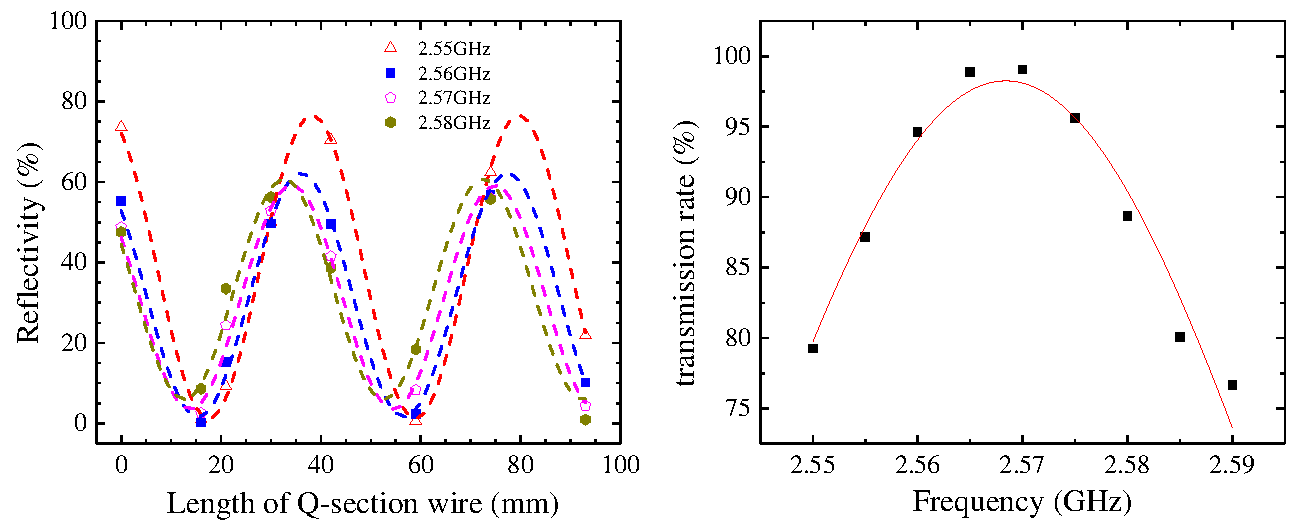
\includegraphics [width =0.95 \linewidth]{Apparatus-loop-antenna_retrun_loss.pdf}
\end{center}
\caption[Test of the return loss by changing the lengths of the Q-sections]{Test the return loss the full-wave loop antenna by changing the length of the Q-section line. Right side shows the band width test which provides a bandwidth of 67 MHz. }  
\label{antenna_return_loss}
\end{figure}

% about 6.8 7.5Ghz coil (done 2021-9-22 11:43:16)
After confirming that the 2.6 GHz coil does work, we built the 7.5 GHz coil, which could also increase the Rabi freq for Rb at high field. This one is similar to the Na coil with a parameter of 4 cm, which is relatively too small even to put it onto the science cell because it will block some part of the MOT beam. So, we choose to sacrifice power by arranging the coil on one edge of the cell, which increases the distance between the coil and atoms to about 3 cm. The best working distance for the 7.5 GHz coil is \(\lambda/4\), i.e. 1 cm, so for 3 cm distance, we get a power of about 1/3 compared to the maximum one. In order to pump atoms to the target state within tens $\mu$s, the required Rabi frequency needs about 10 kHz. Our online test shows a Rabi frequency of 10 kHz, allowing a 50 $\pi$-pulse for fast removing Rb atom from Feshbach molecules. Thanks to this new antenna, we can remove the horn antenna since the coil still works for 6.8 GHz with a transition rate of about \(10\%\), even its impedance matching point is 7.5 GHz. For typical MW evaporation, very little power is enough. Finally, removing the horn antenna leaves us much more space for future building optics layout.

% Rabi (done 2021-10-29 13:15:45)
\begin{figure}[htb]
\begin{center}
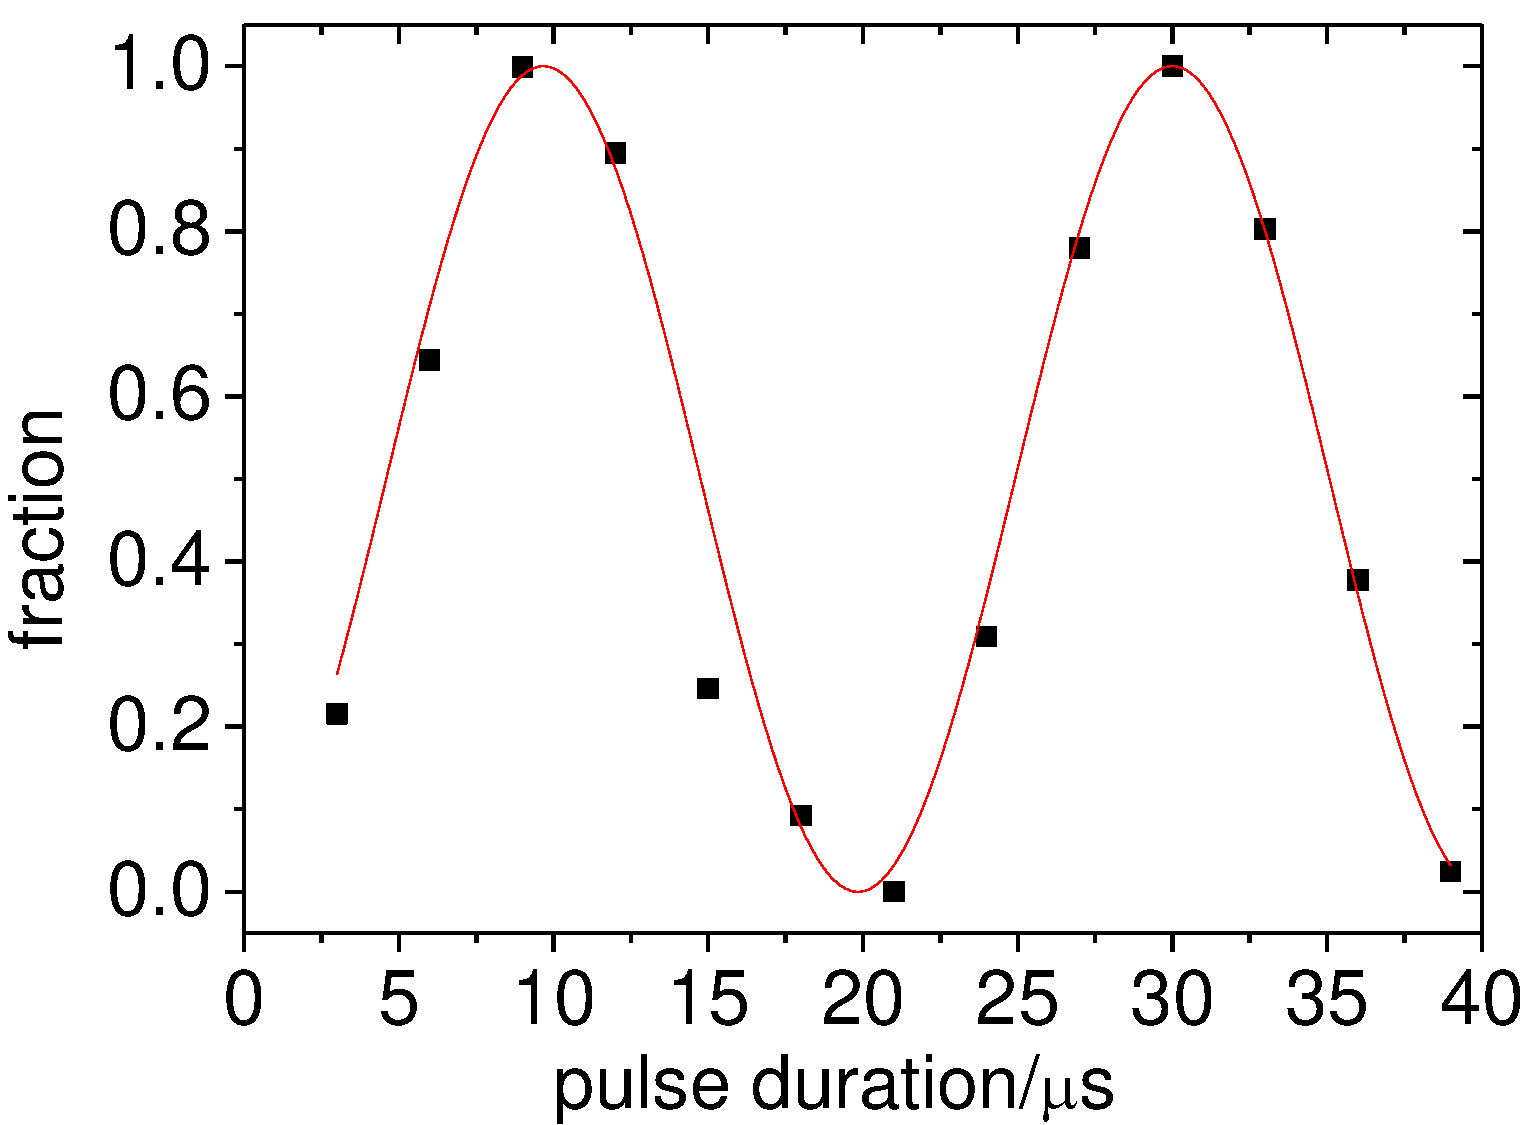
\includegraphics [width =0.7 \linewidth]{antenna_rabi.pdf}
\end{center}
\caption[Test Rabi oscillation of Na $\ket{1,1}$ to $\ket{2,2}$ under 350 Gauss magnetic field]{Test Rabi oscillation of Na $\ket{1,1}$ to $\ket{2,2}$ under 350 Gauss magnetic field. We can achieve a Rabi frequency of 50 kHz, which enable us pump atom to the target cycling transition within 10 $\mu$s.}  
\label{antenna_rabi}
\end{figure}

\chapterend
\chapter{Precision characterisation of a Feshbach Resonance}
\label{Chap_Feshbach}

% epigraph (done: 2021年8月19日13:15:22)
\setlength{\unitlength}{1pt}
\setlength{\epigraphwidth}{11.5cm}
\epigraph{In physical science a first essential step in the direction of learning any subject is to find principles of numerical reckoning and methods for practicably measuring some quality connected with it. \cite{thomson_2011}}{--- William Thomson, 1st Baron Kelvin \\ \textit{Electrical Units of Measurement (1883)}}

\section{Overview}
% Introduction and purpose (done: 2021年8月19日13:19:11)
This chapter presents our precision calibration of a Na-Rb Feshbach resonance at 347.64 G. The purpose of inserting this chapter before discussing the droplet experiment is to require a precision map of the scattering length (actually not only Na-Rb but also Na-Na and Rb-Rb) as a function of the magnetic field. This narrative order is convenient for discussing the droplet experiment; however, the research in chronological order is tortuous as described in Sec. \ref{sec:intro-overview}. I learned my lesson that one should not trust any unverified data. Previous measurements of Feshbach resonance(FR) parameters of Na and Rb, by three-body-loss (3B-loss) spectrum or associating method, both encountered intrinsic systematic errors, such as thermal averaging or shifting \cite{Bartenstein2005, Zurn2013}. Due to the 
high sensitivity of the droplet phase diagram, we need the scattering length map as accurate as possible. So, we implemented the dissociation method to refine the results of FR parameters at 347.64 G resonance. In the rest of this section, we will introduce what Feshbach resonance (FR) is, discuss the previous measurement results, and finally offer the arrangement of this chapter.

% what is a FR and why use FR (done: 2021年8月13日12:45:54)
Feshbach resonance as a powerful toolbox plays its essential role in cold atom experiments. With this nob, we can tune the interaction between atoms by applying an external field. Thus, it is used to explore the few-body (or many-body) physics and form molecules that open a new field in ultracold physics. Feshbach resonance requires two channels to couple to each other. One is the open channel (or entrance channel), with which collision can produce atoms, i.e. the energy of the collision pair is larger than the asymptotic energy of the channel. Another is the closed channel which offers bound states with the set energy instead of scattering state\cite{RevModPhys.82.1225}. When the energy of one bound state in the closed channel approaching the open channel threshold (typically set to be 0), the resonance happens. Near the resonance $B_0$, the two-body scattering length is approximate as
\begin{equation}
a(B) = a_{\rm bg}\left(1+\frac{\Delta}{B-B_0}\right),
\label{FR}
\end{equation}
where $a_{\rm bg}$ is the slowly varying background scattering length, and $\Delta$ is the resonance width. By simply scanning the magnetic field, the scattering length $a$ and thus the effective two-body contact interaction can be changed from repulsive (for $a > 0$) to attractive (for $a < 0$). The capability of manipulating the interaction strengths has been playing a vital role in the study of exotic physics such as the controlled collapse~\cite{donley2001}~or soliton formation in Bose-Einstein condensates (BEC)~\cite{Khaykovich2002,Strecker2002}, the BEC-BCS crossover in quantum-degenerate Fermi gases~\citep{PhysRevLett.92.040403,PhysRevLett.92.120403,Bartenstein2004,Bourdel2004}, and more recently the formation of dilute quantum droplets~\cite{petrov2015,ferrier2016Observation,cabrera2018quantum}. In addition, FRs are used to associate atomic pairs and form weakly bound Feshbach molecules (FMs)~\cite{Kohler2006}. Combined with a subsequent two-photon Raman process, this has led to the creation of long-sought ultracold ground-state molecules~\cite{ni2008,Takekoshi2014,Molony2014,Park2015,PhysRevLett.116.205303,VOGES2020}.

% Na-Rb FR previous measurements (done 2021年8月19日13:50:52)
The typical way of tuning the scattering length by an FR in the cold atom experiment is to control the magnetic field. When the magnetic field is tuned to the vicinity of the resonance, we have a large scattering length, thus can increase the two-body collision rate. This method enables us to enhance the three-body loss rate \cite{wang2013observation}, and by scanning the magnetic field, we can obtain a loss dip (as shown in Fig. \ref{FR_loss}). This phenomenon can be used to characterize an FR directly at first glance. By a simple Gaussian fitting to extract the peak, we obtain the resonance position. The problem of calibrating an FR by this method mainly comes from the existence of lots of Efimov states near the resonance. These three-body bound states render a severe three-body loss and then broaden or shift the measurement of resonance position \cite{RevModPhys.82.1225}. Later in 2015, \cite{wang2015formation} used the association method to calibrate the 347 G and 478 G Na-Rb FR again. However, the asymmetric associating spectrum still reveals the thermal broadening and shifting, leading to inaccuracy measurement of FR parameters \cite{Bartenstein2005, Zurn2013}.

% Show a figure for one FR loss spectrum (done 2021年8月19日13:39:31)
\begin{figure}[htb]
\begin{center}
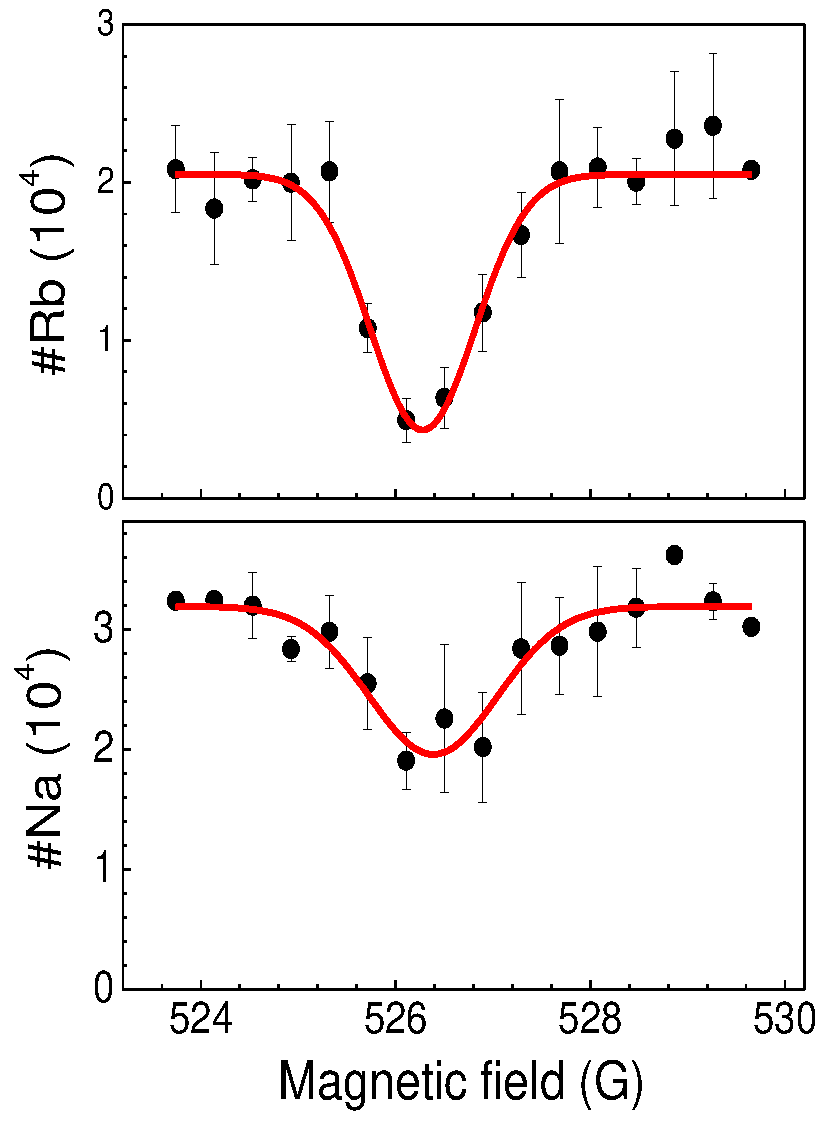
\includegraphics[width = 0.5\linewidth]{FR_loss.pdf}
\end{center}
\caption[One example of loss spectrum of Feshbach resonance.]{shows the loss spectrum of one Feshbach resonance of Na$\ket{F=1,m_F=0}$ and Rb$\ket{F=1,m_F=0}$.}
\label{FR_loss}
\end{figure}

% Introduce the dissociating method (done 2021年8月19日14:16:11)
Thus, in this Chapter, we use the most accurate method, i.e. the dissociating method, to calibrate the FR of Na and Rb at 347.64 G. To obtain an accurate map of scattering length, we need the knowledge of the molecular bound state. Recalling the discussion in chap. \ref{Chap:theory}, when we talk about quantum scattering, we typically use a pseudopotential to substitute the real complex interaction potential. However, we have to go back to the complicated real potential to obtain its scattering properties before having the scattering length. Then, an accurate map of the molecule potential is essential. Historically, people use the hot molecule to get the spectrum and then inversely deduct the potential curve \cite{}. However, this spectrum is typical only for deeply bound molecule states, which contains little information about the weakly bound states and thus the Feshbach resonances. However, our experiments need the scattering length near a Feshbach resonance, related to shallow bound states near or approaching zero when the external magnetic field is tuned across specific values. Thus, similar to the associating method, our goal is clear that we need a method to obtain these bound states energy accurately. However, to avoid the systematic error in the associating method (as shown in Fig. \ref{FR_asso}), we first form a pure molecule sample and then dissociate. Thinking in the coordinate of one molecule, one would find that this dissociation process can avoid thermal effects and thus improve the measurement accuracy. After obtaining the information of bound states, we can fit them by the coupled-channel calculation to get the Na-Rb potential. Finally, we achieve the accurate scattering length map as a function of the magnetic field. 

% Show a figure of association spectrum (done 2021年8月19日15:54:40)
\begin{figure}[htb]
\begin{center}
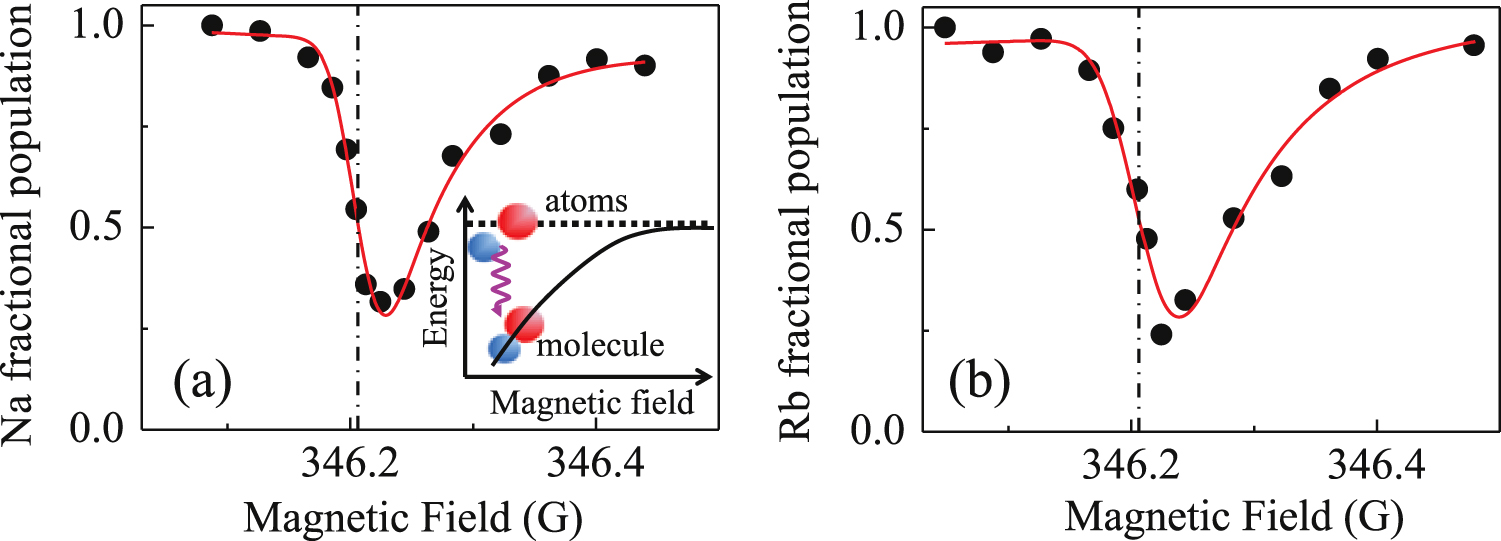
\includegraphics[width = 0.9\linewidth]{FR_asso.jpg}
\end{center}
\caption[Association spectrum of Na and Rb near 347.64 G. (Image from \cite{wang2015formation})]{Image from \cite{wang2015formation}. (a) and (b) shows the Na and Rb residue signal when doing the associating of Feshbach molecules. The dash-dot line shows the association limit, which corresponding to the zero-energy of the bound state. For a magnetic field less than the threshold, there are still association signals indicating the thermal effect. These thermal shifting and broadening smoothen the kink at the associating limit.}
\label{FR_asso}
\end{figure}

% arrangement of this chapter (done 2021年8月19日16:08:42)
The rest of this chapter is arranged as follows: Sec. \ref{sec:cali_FR} describes the method of dissociation measurement of FR molecule binding energy. Then, we apply the coupled-channel (c.c.) calculation fitting the data to obtain an accurate molecule potential curve. Finally, we achieve an accurate scattering length map. In Sec. \ref{sec:FR_spec_more}, we present ten more Feshbach resonance loss spectrums with different spin configurations of Na and Rb. They are compared to a c.c. calculation. We measured most elastic resonances and some of the inelastic, which process imaginary part of scattering length. This information can be used as a map for further exploration of a variety of Bose mixtures. Moreover, in the second part of Sec. \ref{sec:FR_spec_more} we demonstrate c.c. calculations for Rb-Rb and Na-Na both in $\ket{F=1,m_F=1}$ states. We find that the Na intraspecies interaction shows a very smooth variation from 54.5 $a_0$ (at 0 Gauss) to 64 $a_0$ (at around 900 G). This renders our estimation of Na-Na intraspecies scattering length shift about $10\%$ in the droplet paper \cite{guo2021leehuangyang}, from 54.45 $a_0$ to 60.05 $a_0$.

\section{Na-Rb Feshbach resonance at 347.64 G}
\label{sec:cali_FR}

% Method overview (done 2021年8月19日17:03:40)
This section\footnote{Announcement: most materials in this section is from our paper \cite{guo2021tunable}, which could lead to resemblance.} reports new measurements of binding energies for the state that causes the FR near 347.64 G. To reach the highest accuracy, we implement the dissociation method~\cite{Bartenstein2005,Zurn2013,Chin2005radio,Chapurin2019} to measure the binding energies. We achieve magnetic field stability at the mG level. The data are used to refine the interaction potentials for the $X^1\Sigma^+$ and $a^3\Sigma^+$ electronic states by fitting to coupled-channel bound-state calculations. We then use coupled-channel scattering calculations to obtain a highly accurate mapping $a(B)$ for the FR near 347.64~G. This has become a cornerstone for our recent experiment on the heteronuclear Na-Rb~quantum droplet\cite{guo2021leehuangyang}. 

% Method details (done 2021年8月19日17:27:49)
By applying a radio-frequency pulse to drive a bound-free transition~\cite{Bartenstein2005,Zurn2013,Chapurin2019}. The binding energy is obtained by subtracting the free-free transition energy from the bound-free transition energy. In the current work, as shown schematically in Fig.~\ref{FR_dis}(a), the FM lies very close in energy to the free atom pair. In this case, the dissociation can be driven by magnetic field modulation spectroscopy~\cite{Claussen2003,Thompson2005}. As illustrated in Fig.~\ref{FR_dis}(b), this is implemented by adding a small-amplitude oscillation to the magnetic field after the magnetoassociation. The oscillating magnetic field can be expressed as $B+A\times{\rm sin}(2\pi f t)$, with $B$ the final magnetic field that determines $E_{\rm b}$, and $A\ll B_0-B $. $B_0$ is the resonance magnetic field and $f$ is the modulation amplitude and frequency. Dissociation starts to occur when $f$ matches $E_{\rm b}/h$. For $f > E_{\rm b}/h$, the excess energy is converted to kinetic energy of the free atoms as $E_{\rm k} = hf - E_{\rm b}$. Due to the variation of the bound-free Franck-Condon factor with $E_{\rm k}$~\cite{Chin2005radio}, the dissociation spectrum is typically asymmetric and broad with respect to $f$.

% section outlines (done 2021年8月19日17:27:43)
In the rest part of this section, we first detailedly describe experimental measurement. Then, after obtaining the binding energies, we demonstrate the coupled-channel modelling for fitting. Finally, we compare the new calibrated parameters of Feshbach resonance at 347.64 G to the previous measurements.

% dissociation method and time sequence (done 2021年8月19日17:28:20)
\begin{figure}[htb]
\begin{center}
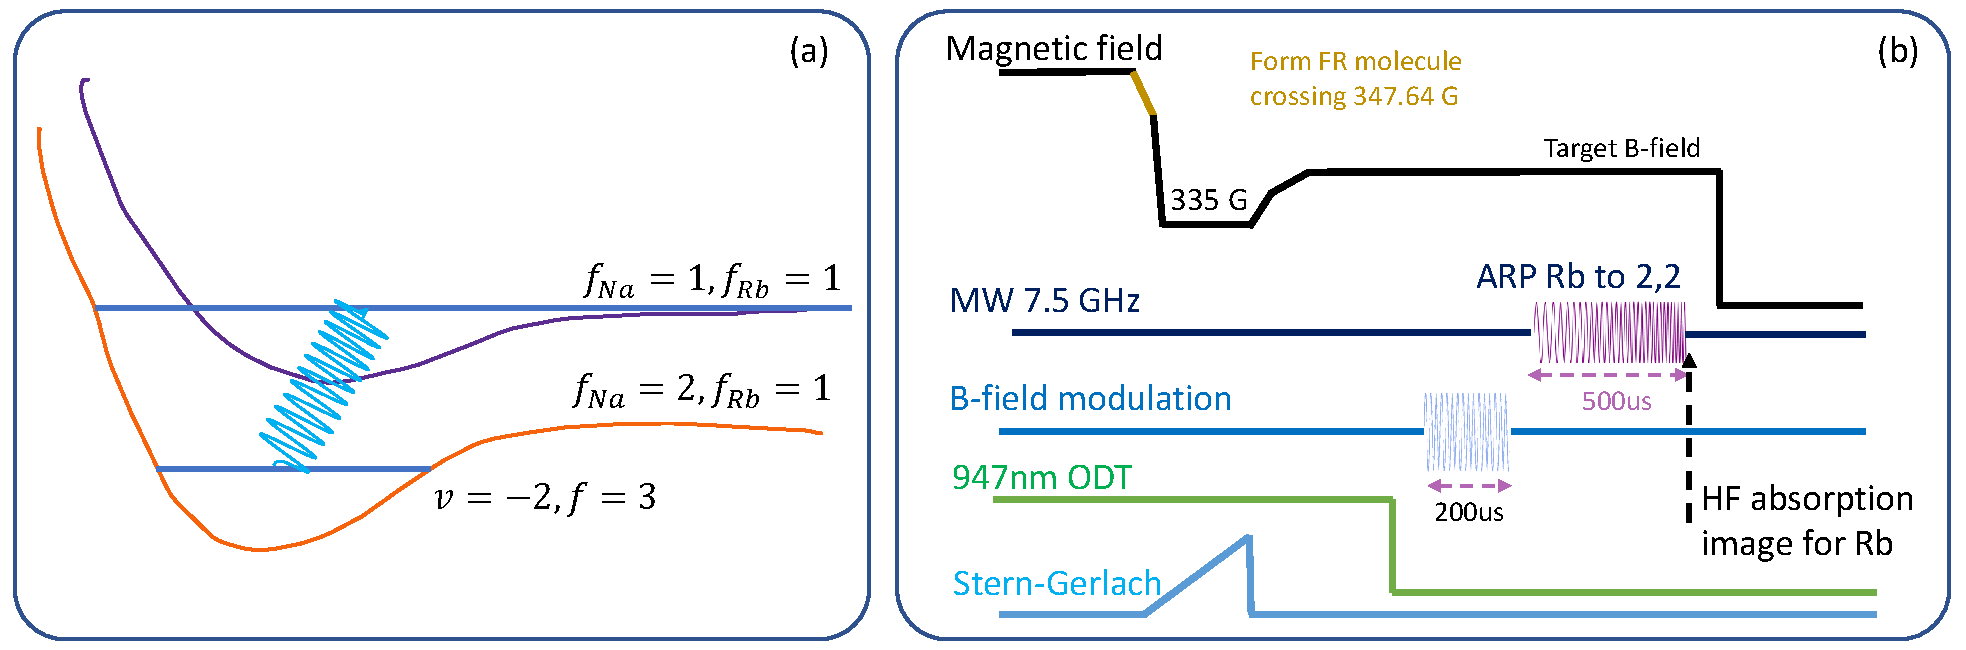
\includegraphics[width = \linewidth]{FR_dis.pdf}
\end{center}
\caption[Time sequence for measuring binding energy of Feshbach molecules]{Measuring the binding energy of a Feshbach molecule with magnetic field modulation spectroscopy. (a) The binding energy of the FM is $E_{\rm b}$. An oscillating magnetic field can drive a bound-free transition. (b) The FMs are first created by ramping the magnetic field across $B_0$. After the magnetic field is stabilized to its final value, a small-amplitude sinusoidal oscillation at frequency $f$ near $E_{\rm b}/h$ is added to dissociate the FMs and measure the binding energy. See the text for a more detailed description of the magnetic field ramping procedure.}
\label{FR_dis}
\end{figure}

\subsection{Measurement of the Na-Rb Feshbach molecule binding energy}

% produce atom to molecule (done 2021年8月19日17:47:03)
Our experiment starts from an optically trapped ultracold mixture of $^{23}$Na and $^{87}$Rb atoms, both in their lowest hyperfine state $\ket{F = 1, m_F = 1}$~\cite{wang2013observation,wang2015formation,jia2020}. Magnetoassociation starts from an initial magnetic field of 350 G, just above the FR at $B_0 = 347.64$ G. The magnetic field is ramped down across the resonance to form FMs, and then to 335.6 G. At this field, the FMs have a nearly zero magnetic dipole moment; this allows us to remove the residual atoms with a short and strong magnetic field gradient without losing molecules. Afterwards, the magnetic field is ramped up to a range of target values below $B_0$ for further experiments. Following this procedure, we can routinely obtain a pure sample of $^{23}$Na--$^{87}$Rb FMs with a typical temperature of 300 nK and a trap lifetime of more than 30 ms. This short lifetime is due to near-resonance photon scattering by the 947 nm optical trap light~\cite{Guo2017,jia2020}, which is provided by a home-built diode laser system. In another experiment on $^{23}$Na--$^{87}$Rb, in which a single-frequency 1064 nm laser is used as the optical trap light, FM lifetimes greater than 100 ms have been observed~\cite{Wang2019,guo2021leehuangyang}. Nevertheless, the current lifetime is more than enough for the present work, as we need only 10 ms for magnetic field stabilization and less than 1 ms for dissociation.

% remove residue atom (done 2021年8月19日21:54:33)
To obtain a high-quality dissociation spectrum, we need a pure molecule sample. If there remain atoms inside the molecule sample, though very few, because the dissociated atoms are few, it is hard to distinguish the dissociated one from the residue one. On the other hand, this part of the atom could be associated to molecules which makes the spectrum hard to subtract information. To remove residue atoms from molecules, we need to identify them by different properties, such as magnetic dipole, mass, transition frequency. To blast atoms away, we need to obtain the acceleration of atoms as large as possible and keep the molecule unaffected. The typical methods can be magnetic gradient, species-dependent optical dipole force (tune-in, tune-out trap) and resonance light for atoms. In our experiment, we originally apply the magnetic gradient at 335 G, where FMs possess zero magnetic dipoles. This method typically requires 1-2 ms to separate atoms all away from molecules, which is slow. The main limitation is the slew rate of coil current due to large coil inductance. So, later we change the method: we first transfer atoms to $\ket{F=2,m_F=2}$~state by light or by MW, then use the image cycling transition to remove the atom. With the newly upgraded full-wave loop antenna, we can achieve a high Rabi frequency for Na and Rb, both up to 50 kHz. Then, a ten us pulse could transfer all atoms to the cycling transition ground state $\ket{F=2,m_F=2}$. Then, the probe light with several saturation-intensity can blast all atoms away within less than 10 $\mu$s. More details can be found in Chap. \ref{Chap_Apparatus}.

% magnetic field modulation method (done 2021年8月19日22:07:29)
The magnetic field modulation is generated by a single loop coil driven by a low-frequency high power radio frequency amplifier. The single loop coil is placed just above the vacuum cell and coaxially with the Feshbach coils so that a modulation depth of several mG can be added to the large magnetic field. The coil has a limited modulation bandwidth of about 2 MHz. The optical trap was turned off 50 $\mu$s before applying the magnetic field modulation pulse to avoid the AC-Stark shift from the trapping light. This also reduces possible systematic errors induced by mean-field shifts of both the FMs and the free atoms as the density of FMs is lowered down. The magnetic field modulation pulse duration is chosen empirically so that the fraction of dissociation is no more than $70\%$. This is a compromise for detection signal-to-noise ratio and the requirement for using the Fermi Golden rule to fit the dissociation lineshape, which is only strictly followed for weak coupling. 

% dissociation curve 
\begin{figure}[htb]
\begin{center}
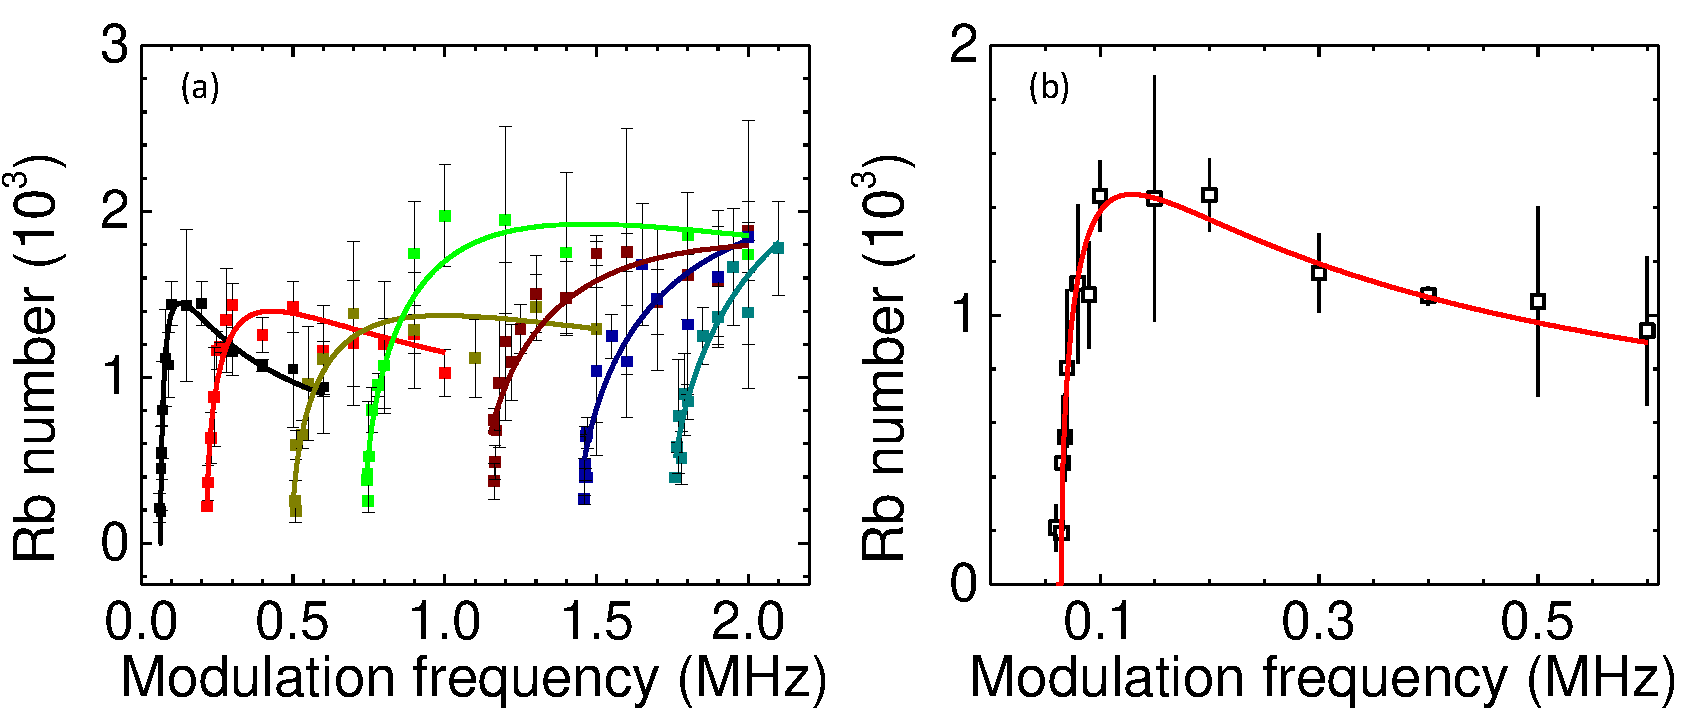
\includegraphics[width = 0.95\linewidth]{FR_spec.pdf}
\end{center}
\caption[Feshbach molecule dissociation spectrum]{Feshbach molecule dissociation spectrum at magnetic field of (a) 347.371 G, and (b) 346.000 G. The red solid curves are fitted to Eq.~\ref{eq2} to extract the FM binding energies. Because of the limited modulation bandwidth of the single-loop coil, only part of the spectrum is accessible in (b).}
\label{FR_spec}
\end{figure}

% dissociation signal (done 2021年8月21日20:22:49)
The dissociation signal is detected by absorption imaging of the fragmented $^{87}$Rb atoms. Fig.~\ref{FR_spec}(a) shows several examples of dissociation spectrum versus the modulation frequency $f$ for FMs from 347.371(5) G to 345.713(5) G. Here the magnetic field is measured with radio frequency spectroscopy of the Rb atoms. Threshold behaviors are clearly visible in all dissociation spectra. Fig.~\ref{FR_spec}(b) shows the enlargement of 347.371 G dissociation spectrum in (a). There is no dissociation is observed for $f$ below 60 kHz. Since the dissociation process involves no moment transfer, the dissociation threshold is an accurate measurement of the binding energy $E_b$ of the FM. Above this threshold, the profile of the spectrum is determined by the overlap between the wave functions of the bound and free states. As the excessive energy $hf-E_b$ will be converted into the relative motion of the two atoms, the wave function of the free atoms and thus the bound-free transition rate changes with $f$. Following~\cite{Mohapatra2015}, the lineshape of magnetic field modulation spectroscopy can be represented as
\begin{equation}
N_{Rb}(f) \propto \frac{\sqrt{hf-E_b}}{hf}.
\label{eq2}
\end{equation}
From this lineshape, a dissociation maximum should be observed at $f = 2E_b/h$, afterwards, the signal will decay with a long tail following $1/\sqrt{f}$. The spectrum in Fig.~\ref{FR_spec}(b) follows this lineshape well. For the spectrum with $E_b>1$~MHz in Fig.~\ref{FR_spec}(a), the maximum is not reached due to the limited modulation bandwidth. 

% subtract kink point, i.e. the binding energy (done 2021年8月21日20:30:58)
To determine the dissociation threshold, we fit each spectrum with Eq.~\ref{eq2}. For partial dissociation spectra like Fig.~\ref{FR_spec}(b), we have verified with simulated data that $E_{\rm b}$ can still be determined with uncertainties less than 5 kHz. The variation of $E_{\rm b}$ with magnetic field, over a range from 0.061 MHz to 1.739 MHz, is plotted in Fig.~\ref{FR_bind} as black open circles. The error bar for each $E_{\rm b}$ is smaller than the symbol size. The uncertainty in the measured magnetic field is $\pm3$~mG. 

%%% Binding energy vs. Magnetic field (done 2021年8月22日11:34:39)
\begin{figure}[htbp]
\begin{center}
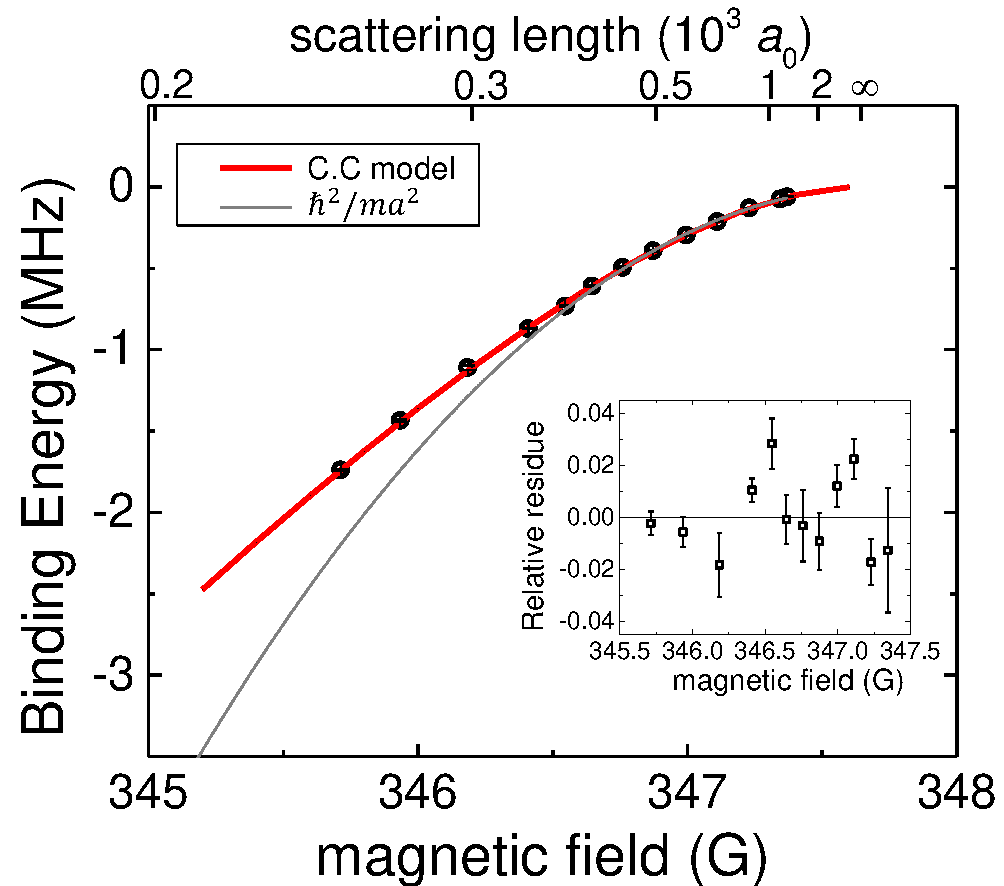
\includegraphics[width = 0.9\linewidth]{FR_bind.pdf}
\end{center}
\caption[Binding energy of $^{23}$Na$^{87}$Rb Feshbach molecules at 347.64 G]{Binding energy of $^{23}$Na$^{87}$Rb Feshbach molecules created via the FR near 347.64 G in the entrance channel Na$\ket{1,1}$+Rb$\ket{1,1}$. The black open circles are the data points measured with the dissociation method. The error bars are smaller than the symbol size. The solid red curve is from the coupled-channel (c.c.) fitting, while the thin black curve is from the universal model. Inset shows the relative residue between the experiment data and the c.c. fitting.}
\label{FR_bind}
\end{figure}

% compare association method and dissociation method (done 2021年8月22日12:05:27)
Figure~\ref{FR_asso} shows $E_{\rm b}$ for FMs that were obtained in 2015 with the association method\cite{wang2015formation} near the resonances at 347.64 G. In that work~\cite{wang2015formation}, the binding energy was fitted using the square-well model~\cite{Lange2009} with a fixed background scattering length $a_{\rm bg} = 66.77a_0$. This value of $a_{\rm bg}$ was obtained from the coupled-channel modelling of the several Feshbach resonances observed with atom-loss spectroscopy in 2013~\cite{wang2013observation}. However, the square-well model requires $a_{\rm bg}$ much larger than the interaction range, which is set by the mean scattering length of the van der Waals potential \cite{Gribakin1993}; this is $\bar{a} = 55.2\,a_0$ for $^{23}$Na$^{87}$Rb. This condition is not satisfied for the Feshbach resonances considered here. It is also well known that resonance positions measured by atom-loss spectroscopy are not accurate enough due to the complicated dynamics of three-body recombination. These issues all contribute to the inaccuracy of the Feshbach resonance parameters determined previously~\cite{wang2015formation}. In the following, we solve these issues with a new coupled-channel modelling of the binding energies of the FMs.

\subsection{Coupled-channel modeling and Feshbach resonance parameters}
\label{sec:cc}

% introduction about method of calibration molecular potential (done 2021年8月22日17:49:00)
After obtaining the Feshbach molecule's binding energy, we measure out how the highest shallow bound state energy varies with the magnetic field. This very shallow bound state is affected mainly by the shortest part and the long-range part ($C_6$, $C_8$, $C_{10}$) of the molecular potential curve. So, by the above measurement, we can calibrate the potential more precisely, especially at short and long-range since a typical molecular potential is achieved by the Fourier-transform molecular spectroscopy\cite{Pashov2005}, which mainly use the information for the deep binding bound state, i.e. middle range potential. We can achieve a more accurate molecular potential for Na and Rb by combining the spectroscopy data for mid-range and the measurement of shallow bound state for short and long-range. 

% what is c.c. calculation (done 2021年8月22日18:11:18)
Coupled-channel calculations rely on expanding the total wavefunction for a pair of interacting atoms in a basis set that represents the electron and nuclear spins and the relative rotation of the atoms (the partial wave $L$). Substituting this expansion into the total Schr\"odinger equation produces a set of coupled differential equations that can be solved to obtain either bound-state or scattering properties. The Hamiltonian for the interacting pair is
\begin{equation}
\label{full_H}
\hat{H} =\frac{\hbar^2}{2\mu}\left[-\frac{1}{R}\frac{d^2}{dR^2}R
+\frac{\hat{L}^2}{R^2}\right]+\hat{H}_\textrm{A}+\hat{H}_\textrm{B}+\hat{V}(R),
\end{equation}
where $R$ is the internuclear distance, $\mu$ is the reduced mass, and $\hbar$ is the reduced Planck constant. $\hat{L}$ is the two-atom rotational angular momentum operator. The single-atom Hamiltonians $\hat{H}_i$ contain the hyperfine couplings and the Zeeman interaction with the magnetic field. The interaction operator $\hat{V}(R)$ contains the two isotropic Born-Oppenheimer potentials, for the $X^1\Sigma_g^+$ singlet and $a$ $^3\Sigma_u^+$ triplet states, and anisotropic spin-dependent couplings which arise from dipole-dipole and second-order spin-orbit coupling. In the present work, scattering calculations are carried out using the MOLSCAT package
\cite{molscat:2019,mbf-github:2020} and bound-state calculations use the related packages BOUND and FIELD \cite{mbf-github:2020}. The scattering wavefunction is expanded in a fully uncoupled basis set that contains all allowed spin and rotational functions, limited by $L_{\rm max}=2$. The numerical methods are similar to those used in Ref.\ \cite{Berninger:Cs2:2013}, so will not be described in detail here.

% molecular potential structure (done 2021年8月22日18:11:15)
The interaction potential used here is based on the potential curves for the $X^1\Sigma^+$ and $a^3\Sigma^+$ states of NaRb, originally obtained by fitting to Fourier transform (FT) molecular spectroscopy~\cite{Pashov2005} and later refined by Feshbach spectroscopy with ultracold atoms~\cite{wang2013observation}. The potential curve for each electronic state, with spin $S=0$ (singlet) or 1 (triplet), has three parts: (1) a high-order power-series in the well region, which is the part best determined by FT spectroscopy; (2) a long-range extrapolation, outside internuclear distance $R_{{\rm LR},S}$, which uses theoretical dispersion coefficients and a simple exchange term; (3) a short-range extrapolation, inside $R_{{\rm SR},S}$, which uses a simple repulsion of the form $A_S + B_S/R^N_S$. $R_{{\rm SR},S}$ is usually chosen as a distance just outside the inner turning point of the potential at zero energy. For particular values of $R_{{\rm SR},S}$ and $N_S$, $A_S$ and $B_S$ are usually determined so that the short-range extrapolation has the same value and derivative at $R_{{\rm SR},S}$ as the mid-range power-series potential \footnote{This constraint was applied in the present work, but for the potential of Ref.\ \cite{wang2013observation} there are derivative discontinuities at $R_{{\rm SR},S}$.}.

% fitting to get new potential (done 2021年8月22日18:11:35)
Our goal is to adjust the interaction potential to fit the measured FM binding energies, while retaining as much as possible its ability to reproduce the FT spectra. We therefore keep the two power series that represent the singlet and triplet potential wells fixed at the fitted values of Ref.\ \cite{wang2013observation}. We also retain the long-range extrapolation in its original form, with the dispersion coefficients unchanged. We vary only the parameters $R_{{\rm SR},S}$ and $N_S$ that define the short-range extrapolations. For the triplet potential, $R_{{\rm SR},1}$ is held at its original value from Ref.\ \cite{wang2013observation}, and $N_1$ is varied; this provides sufficient flexibility to adjust the singlet scattering length and reproduce resonance positions and binding energies. For the singlet potential, however, the original value of $R_{{\rm SR},0}$ is so close to the turning point that varying $N_0$ does not allow enough change in the potential to reproduce the experimental data. In this case $N_0$ is held at its original value from Ref.\ \cite{wang2013observation}, and $R_{{\rm SR},0}$ is varied.

% add potential parameters
Here attaches the new potential parameters for Na and Rb $X^1\Sigma_g^+$ singlet and $a$ $^3\Sigma_u^+$ triplet states.
\lstset{
    backgroundcolor=\color{backcolour},   
    commentstyle=\color{codegreen},
    keywordstyle=\color{magenta},
    numberstyle=\tiny\color{codegray},
    stringstyle=\color{codepurple},
    basicstyle=\ttfamily\footnotesize,
    breakatwhitespace=false,         
    breaklines=true,                 
    captionpos=b,                    
    keepspaces=false,                 
    numbersep=5pt,                  
    showspaces=false,                
    showstringspaces=false,
    showtabs=false,                  
    tabsize=2
}
\linespread{1.0}
\begin{lstlisting}
Analytic potential energy curve for the NaRb a3Sigma+ state
(for definition of parameters see C. Samuelis et al. PRA 63, 012710 (2000)) 
-------------------------------------
Potential is given with respect to the dissociation limit which is set to 0!

For R <= 4.65 A

U(R)=A+B/R^alpha

A	-232.9656123524    cm-1
B	10710621685.47      cm-1 A^alpha 
alpha       11.492

For 4.65 < R < 11.30 A

U(R)=Sum_i[a_i*((R-R_m)/(R+b*R_m))^i]

b     -0.4700
R_m   5.60071538 A 
a_0  -203.35070852 cm-1
a_1   0.122517410860683240E+01 cm-1
a_2   0.968561681714175506E+03 cm-1
a_3  -0.167358901820848331E+03 cm-1
a_4  -0.115108986132623340E+04 cm-1 
a_5   0.538103153477437104E+03 cm-1
a_6   0.576427139041465671E+04 cm-1
a_7  -0.137759208524156093E+05 cm-1
a_8  -0.484354206699185452E+05 cm-1
a_9   0.876873287464803143E+05 cm-1
a_10  0.242372373596938676E+06 cm-1
a_11 -0.283727768851481727E+06 cm-1
a_12 -0.762367745318190078E+06 cm-1
a_13  0.433100100910781766E+06 cm-1
a_14  0.150133971696866141E+07 cm-1
a_15 -0.489081569236799405E+05 cm-1
a_16 -0.164041059210233274E+07 cm-1
a_17 -0.680259713656829204E+06 cm-1
a_18  0.665168317123337765E+06 cm-1
a_19  0.606016435356653412E+06 cm-1
a_20  0.137434664322447614E+06 cm-1
  
For R>=11.30 A

U(R)=-C_6\R^6-C_8\R^8-C_10\R^10+A_ex*R^gamma*exp(-beta*R)

C_6    0.129463596372576691E+08 cm-1 A^6
C_8    0.358980000000000000E+09 cm-1 A^8
C_10   0.130601455102733498E+11 cm-1 A^10
A_ex   0.31859846D+05 cm-1 A^(-gamma)
gamma  5.00810   
beta   2.20850 A^-1

--------------------------------
Analytic potential energy curve for the NaRb X1Sigma+ state
(for definition of parameters see C. Samuelis et al. PRA 63, 012710 (2000) 
--------------------------------
Potential is given with respect to the dissociation limit which is set to 0!

For R <= 2.7256 A

U(R)=A+B/R^alpha

A           -8490.090071421    cm-1
B           450828.6299011      cm-1 A^alpha 
alpha   4.06143861049682720

For 2.7256 < R < 11.30 A

U(R)=Sum_i[a_i*((R-R_m)/(R+b*R_m))^i]

b     -0.2100
R_m    3.64340736 A
a_0   -5030.50869783 cm-1
a_1   -0.662030723944292271E-01 cm-1
a_2    0.253807725995464061E+05 cm-1
a_3    0.929104757521979809E+04 cm-1
a_4   -0.211814748606123285E+05 cm-1
a_5   -0.284181834656136671E+05 cm-1
a_6    0.210407753693068798E+04 cm-1
a_7   -0.851968733976350748E+06 cm-1
a_8   -0.123216494098773529E+07 cm-1
a_9    0.383640579108661637E+08 cm-1
a_10   0.109125343263982777E+08 cm-1
a_11  -0.109331126199059677E+10 cm-1
a_12   0.540863749615297675E+09 cm-1
a_13   0.203930014933835602E+11 cm-1
a_14  -0.222458146577416687E+11 cm-1
a_15  -0.258727375257563232E+12 cm-1
a_16   0.419458345047378906E+12 cm-1
a_17   0.226157469213112939E+13 cm-1
a_18  -0.493156268638760059E+13 cm-1
a_19  -0.133732693094783848E+14 cm-1
a_20   0.391427433409150078E+14 cm-1
a_21   0.491914424477468672E+14 cm-1
a_22  -0.214673998282790187E+15 cm-1
a_23  -0.736821254504513125E+14 cm-1
a_24   0.806693583557253000E+15 cm-1
a_25  -0.249784752437157937E+15 cm-1
a_26  -0.198517974510287375E+16 cm-1
a_27   0.172480088271182725E+16 cm-1
a_28   0.281094984850021900E+16 cm-1
a_29  -0.441448085841028300E+16 cm-1
a_30  -0.122221795646213325E+16 cm-1
a_31   0.552071157529799900E+16 cm-1
a_32  -0.210051881065563800E+16 cm-1
a_33  -0.244906408631624500E+16 cm-1
a_34   0.238499017935224850E+16 cm-1
a_35  -0.611040299017092875E+15 cm-1

For R>=11.30 A

U(R)=-C_6\R^6-C_8\R^8-C_10\R^10-A_ex*R^gamma*exp(-beta*R)

C_6    0.129463596372576691E+08 cm-1 A^6
C_8    0.358980000000000000E+09 cm-1 A^8
C_10   0.130601455102733498E+11 cm-1 A^10
A_ex   0.31859846E+05 cm-1 A^(-gamma)
gamma  5.00810   
beta   2.20850 A^-1
\end{lstlisting}

% continuing (done 2021年8月22日18:12:09)
The shape of the curve of $E_{\rm b}$ as a function of $B$ is quite insensitive to variations in the singlet and triplet scattering lengths, represented by $R_{{\rm SR},0}$ and $N_1$. It is therefore sufficient to fit to one binding energy from each FR. For the resonance near 347.64 G, we choose the point with $E_{\rm b}/h = 0.611(6)$~MHz at 346.646(5) G, while for the resonance near 478.7 G, we choose the point with $E_{\rm b}/h = 0.400$~MHz at 478.052(10) G. The parameters $R_{{\rm SR},0}$ and $N_1$ are then adjusted so that these binding energies are reproduced essentially exactly. The resulting values are $R_{{\rm SR},0}=2.7256$~\AA\ and $N_1=11.492$. The singlet and triplet scattering lengths calculated from the fitted potentials are  $a_{\rm s} = 106.474 a_0$ and $a_{\rm t} = 68.864 a_0$, respectively. These are $0.27 a_0$ smaller and $0.24 a_0$ larger than the values of Ref.\ \cite{wang2013observation}, indicating that the triplet potential needs to be slightly more repulsive than the original at short range, while the singlet potential needs to be slightly less repulsive.

% obtain FR parameters (done 2021-8-22 18:12:32)
We use the fitted potentials to calculate the $s$-wave scattering length $a(B)$. We find that each resonance is well represented by Eq.~\ref{FR}. The parameters $B_{0}$, $\Delta$ and $a_{\rm bg}$ are obtained as described by Frye and Hutson \cite{Frye2017}, and are given in Table~\ref{tab1}. In Fig.~\ref{FR_bind}, the binding energies calculated from the universal model $E_{\rm b} = \hbar^2/2\mu a(B)^2$ using the new $a(B)$ is also shown. Compared with the coupled channel results (red solid curve), this reproduces the data only for $E_{\rm b}< 0.6$ MHz. 

% Parameters of the two low-field $s$-wave Feshbach resonances (done 2021年8月19日22:40:53)
\begin{table}[htb]
\caption{Parameters of the two low-field $s$-wave Feshbach resonances for the entrance channel Na$\ket{1,1}$+Rb$\ket{1,1}$.}
\label{tab1}\centering
\begin{tabular}{ c | c | c | c }
\hline\hline
$B_0$ (G) & $\Delta$ (G) & $a_{\rm bg}$ ($a_0$) & reference\\
\hline
347.648 & 4.255  & 76.33 & this work\\
347.64 & 5.20  & 66.77 & \cite{wang2015formation}\\
347.75 & 4.89  & 66.77 & \cite{wang2013observation}\\
\hline
478.714 & 3.491  & 71.55 & this work\\
478.83 & 4.81  & 66.77 & \cite{wang2015formation}\\
478.79 & 3.80  & 66.77 & \cite{wang2013observation}\\
\hline \hline
\end{tabular}
\end{table}

% comparison(done 2021-8-22 18:18:23)
In the present fit, the resonance near 347.64 G has shifted by about 0.08 G compared to Ref.\ \cite{wang2013observation}. The resonance near 487.7 G has shifted by more than 0.1 G. These shifts produce substantial changes in the calculated scattering lengths. Moreover, in Ref.\ \cite{wang2013observation}, the calculated scattering length was fitted using the formula
\begin{equation}
a(B)=a_{\rm bg} \left[1 + \frac{\Delta_0}{B-B_0} + \frac{\Delta_1}{B-B_1} + \dots\right],
\label{eq:FRsum}
\end{equation}
with a single $B$-independent background scattering length $a_{\rm bg}$ for all resonances. This formula breaks down when the background scattering length varies significantly between resonances. In the present work, Eq.~\ref{FR} is found to be a good local representation for each resonance, but significantly different values of $a_{\rm bg}$ are needed for the resonances at 347.64 G and 487.7 G. Such behavior can arise from many sources, including the changing spin character of atomic states with magnetic field and the presence of additional resonances not included in the summation of Eq.\ \ref{eq:FRsum}. As shown in Fig.~\ref{FR_para}, for the resonance near 347.64 G, the scattering lengths calculated with the new potential differ by about $20a_0$ from those of Ref.\ \cite{wang2015formation} in the region from 349.8 G to 350.0 G that is important for studies of Na-Rb quantum droplets. This change is significant and largely explains the discrepancies initially observed between experiment and theory in Ref.\ \cite{guo2021leehuangyang}.



%%% Binding energy vs. Magnetic field (done 2021年8月22日18:18:11)
\begin{figure}[htbp]
\begin{center}
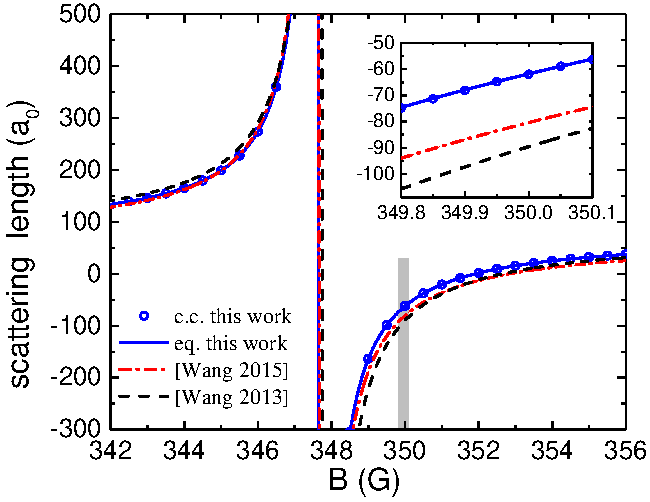
\includegraphics[width = 0.9\linewidth]{FR_para.pdf}
\end{center}
\caption[Scattering length as function of magnetic field]{Comparison of the mapping between magnetic field and scattering length with Feshbach resonance parameters obtained in this work, using coupled-channel results directly (blue open circles) and fitted to Eq.~\ref{FR} (blue solid curve) and , and in Ref.~\cite{wang2015formation} (red dash-dotted curve) and Ref.~\cite{wang2013observation} (black dashed curve), both using Eq.~\ref{eq:FRsum}. The region of interest for the droplet experiment~\cite{guo2021leehuangyang}, marked with a vertical gray bar, is enlarged in the inset. }
\label{FR_para}
\end{figure}

% some explanation for c.c. (done 2021年8月22日18:18:55)
All the coupled-channel calculations use a basis set that includes functions for partial waves $L = 0$ and $L =2$, with the effective dipolar coupling function of Ref.\ \cite{wang2013observation} unchanged. Omitting the $L = 2$ basis functions causes shifts that are on the same level as the experimental uncertainties: the calculated resonance positions and binding-energy curves shift down by between 3 and 4 mG. It is possible to include additional partial waves, but we expect the shifts to be very small. In contrast to Ref.\ \cite{wang2013observation}, we do not include any variation of the atomic hyperfine coupling with internuclear distance.


\section{Na-Rb, Na-Na and Rb-Rb scattering lengths summery}
\label{sec:FR_spec_more}
% overview (done 2021-8-22 18:37:21)
Besides the Feshbach resonance at 347.64 G, different combinations of the spin state of Na and Rb possess plenty of FRs. Ref.~\cite{wang2013observation} investigated the entrance channels $\ket{m_F=1}+\ket{m_F=1}$ and $\ket{m_F=-1}+\ket{m_F=-1}$ and in total observed three $s$-wave and two $p$-wave FRs. In addition, ten more $s$-wave FRs were predicted for collisions between pairs of atoms in different $F = 1$ hyperfine Zeeman states. In this section, we report the experimental observation of several of these FRs below 1000 G in 5 hyperfine Zeeman combinations. We believe these FRs will find important applications in the future, for example, in the investigation of BEC mixtures and quantum droplets with more than two components~\cite{ma2021}. 

% some words on the Na-Na scattering length (done)
With the powerful tool, MOLSCAT \cite{molscat:2019,mbf-github:2020}, we can get more precise maps of scattering length and magnetic field. Since even the background scattering length varies when the external field changes, the value of the scattering length, especially for a finite (not low) field, should be treated with more care. Here we find that the Na-Na 1,1 state have a smoothly varying background scattering length from low field to around 900 G (near the FR). Its value starts from 54.45 $a_0$ to about 64 $a_0$. For our droplet experiment, under about 350 G magnetic field, the Na-Na scattering length is 60.05 $a_0$ which is larger about 10\% than at low field.

\subsection{Na-Rb scattering length for different spin combination}

% experiment preparation state (done 2021-8-22 18:52:27)
For simplicity, we will denote the collision channel of a pair of $^{23}$Na+$^{87}$Rb atoms by $\ket{m_F^{\rm Na}}+\ket{m_F^{\rm Rb}}$. In ref.~\cite{wang2013observation}, both the $\ket{1}+\ket{1}$ and the $\ket{-1}+\ket{-1}$ channels were investigated and in total 3 $s$-wave and 2 $p$-wave FRs were observed. As shown in Fig. \ref{FR_more}, we detect more FRs in different combinations. The experiment for this section starts from optically trapped thermal mixtures of Na and Rb both in the $\ket{-1}+\ket{-1}$ channel. The number of atoms for both species are typically around $10^5$ and the sample temperatures are about 1~$\mu$K. The atoms are then transferred to selected hyperfine Zeeman levels with radio frequency (rf) rapid adiabatic passages. For each species, the $\ket{-1}\rightarrow \ket{0}$ and the $\ket{0}\rightarrow \ket{1}$ Zeeman splittings are very similar. In addition, these splittings in different species are also very similar to each other. To avoid cascade transitions and to realize species-selective state control, the state transfers are performed at 100 G where the transitions are all different by more than 500 kHz. With this method, we are able to prepare the Na-Rb mixture in all the 9 possible $m_F$ combinations of their $F = 1$ states. Then, we ramp the magnetic field to different values and hold the samples for 50 ms before releasing the atoms from the optical trap and measuring the remained numbers of atoms. Intersperses FRs manifest as losses of atoms in both $^{23}$Na and $^{87}$Rb~atoms as a result of enhanced interspecies three-body recombination rates. As presented in Fig.~\ref{FR_more}, guided by the predictions in~\cite{wang2013observation}, we observe 10 FRs in 6 hyperfine Zeeman combinations. 

%%% figure of 10 more FR spectroscopy (done 2021年8月22日18:52:16)
\begin{figure}[htb]
\begin{center}
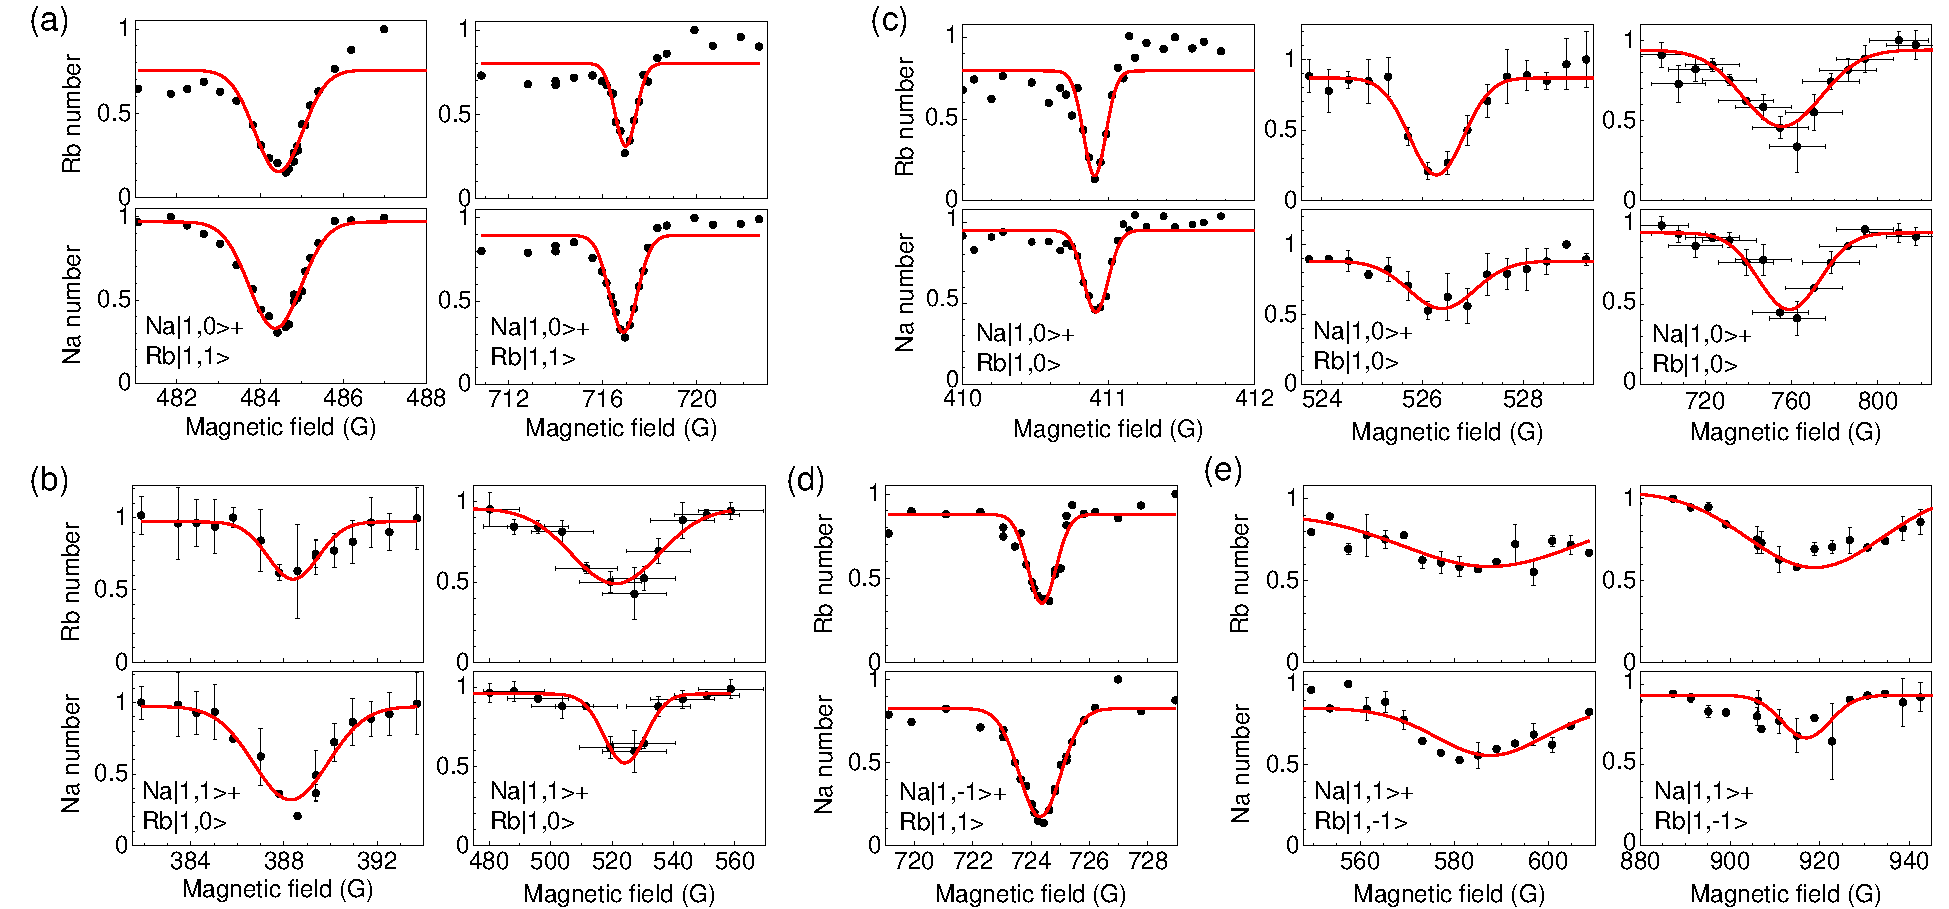
\includegraphics[width = \linewidth]{FR_more.pdf}
\end{center}
\caption[Loss spectroscopy of Feshbach resonance with different spin combinations]{Feshbach resonances in $^{23}$Na-$^{87}$Rb, observed by losses for atoms in the $F = 1$ hyperfine states. (a) and (b) are for the two channels in the $M_F = 1$ manifold; (c), (d) and (e) are for the three channels in the $M_F = 0$ manifold. The typical holding time at each magnetic field is 50 ms. The solid curves are from Gaussian fitting to determine the lineshape center. Error bars for the atom numbers represent one standard deviation. The large error bars for the magnetic field for the several broad loss spectra are due to less precise magnetic field control in these cases (see text).}
\label{FR_more}
\end{figure}

% implement c.c. calculation (done 2021年8月23日10:09:31)
We have carried out coupled-channel calculations of resonance parameters for both elastic and decayed resonances, using the interaction potentials obtained in Sec.~\ref{sec:cc}. The results are included in Table~\ref{fst}. For elastic resonances, the resonance positions for the lowest threshold of each $M_F$ is first located with the FIELD program~\cite{mbf-github:2020}. The FRs are then characterized using the MOLSCAT program~\cite{molscat:2019,mbf-github:2020} following the elastic procedure of Ref.~\cite{Frye2017}, which converges on the resonance position $B_0^{\rm cc}$, the elastic resonance width $\Delta$, and the background scattering length $a_{\rm bg}$. Here $a_{\rm bg}$ is a local background scattering length that is different for each resonances. In the current calculation, we have not included the spin-spin interaction, so that both the quantum number $L$ of the partial wave and its projection $M_L$ are conserved in the calculation. Since $M_{\rm tot} = m_F^{\rm Na}+m_F^{\rm Rb} + M_L$ is conserved, only closed channels with $M_F = m_F^{\rm Na}+m_F^{\rm Rb}$ the same as the colliding atoms can cause FRs.

% FR spectroscopy and c.c. calculation table (done 2021年8月23日10:11:19)
\begin{sidewaystable}[thp]
\caption[Summary table of Na-Rb Feshbach resonances with different spin combinations]{Comparison of experimental resonance positions $B_0^{\rm exp}$ with theoretical parameters for interspecies FRs below 1000 G in $^{23}$Na-$^{87}$Rb, for the nine $F = 1$ entrance channels. $L$ indicates the partial wave of the entrance channel. $B_0^{\rm exp}$ is the mean of the centers of the loss spectra for $^{23}$Na and $^{87}$Rb in Fig.~\ref{FR_more}, determined by Gaussian fitting. Error bars represent one standard deviation. The theoretical values are from coupled-channel calculations using the singlet and triplet potential-energy curves described in Sec.~\ref{sec:cc} with the latest potential parameters. $B_0^{\rm cc}$, $\Delta$, and $a_{\rm bg}$ are the theoretical position, elastic width, and background scattering length, respectively. The last column ``inel.?'' indicates whether the FR is subject to inelastic losses from spin exchange. For decayed FRs with inelastic losses, the resonant scattering length $a_{\rm res}$ and the inelastic width $\Gamma_{\rm inel}$ are also listed.}
\label{fst}\centering
\begin{tabular}{l|c|l|c|c|c|c|c|c}
\hline\hline
Entrance channel 				& $L$ & $B_0^{\rm exp}$(G)	& $B_0^{\rm cc}$(G)	& $\Delta$(G)	& $a_{\rm bg}$($a_0$) & $a_{\rm res}$($a_0$) & $\Gamma_{\rm inel}$(G)	& inel.? \\
\hline
Na$\ket{1,1}$ + Rb$\ket{1,1}$   & 0    	& 347.61(2)       	& 347.645 			& 4.258  			 & 76.328  	& & & N     \\
					        	& 0 	& 478.82(3)        	& 478.712 			& 3.495  			 & 71.548   & & & N     \\ \hline
Na$\ket{1,1}$ + Rb$\ket{1,0}$   & 0    	& 388.5(2)          & 388.577 			& 5.684  & 78.441                 &6548.8 & $-0.13617$& Y     \\
								& 0    	& 522(10)           & 524.286 			& 1.010  & 74.332                 & 12.906& $-11.634$& Y     \\ \hline
Na$\ket{1,0}$ + Rb$\ket{1,1}$   & 0   	&  	--		        & 358.078 			& <0.001  & 80.108                & & & N     \\
								& 0   	& 484.45(5)         & 484.569 			& 4.476  & 77.258                 & & & N     \\
								& 0		& 	--				& 570.441			& <0.001	& 73.784			 & & & N \\
								& 0   	& 716.97(6)         & 717.166 			& 5.593  & 72.998                 & & & N     \\  \hline
Na$\ket{1,1}$ + Rb$\ket{1,-1}$ 	& 0    	& 587(3)         & 580.686 			& 0.241  & $82.389 - 0.0072 i $  & $2.3917 + 0.87566 i$&$-16.596$& Y     \\
							  	& 0    	& 920(1)         & 913.431 			& 0.091  & $81.139 + 0.0352 i$ & $0.47768 + 0.12885 i$& $-30.861$& Y     \\ \hline
Na$\ket{1,0}$ + Rb$\ket{1,0}$  	& 0    	& 410.90(1)         & 409.810 			& 0.176  & 82.328                 & & & N     \\
    							& 0    	& 526.29(3)         & 526.548 			& 5.676  & 78.132                 &23515 &$-0.03772$ & Y     \\
    							& 0    	& 759(13)           & 768.781 			& 1.638  & 75.495                 &19.983 &$-12.373$ & Y     \\ \hline
Na$\ket{1,-1}$ + Rb$\ket{1,1}$ 	& 0    	& --		        & 419.648 			& <0.001  & 80.109                &0.25533 &$-0.34477$ & Y     \\
								& 0    	& --        		& 516.986 			& 0.003  & 79.401                 & & & N     \\	
								& 0    	& 724.38(4)         & 727.270 			& 4.870  & 76.444                 & & & N     \\ \hline
Na$\ket{1,0}$ + Rb$\ket{1,-1}$  & 0    	& --          		& -- 			& -- & --                             & & & N     \\ \hline
Na$\ket{1,-1}$ + Rb$\ket{1,0}$  & 0    	& --          		& 609.754 			& 0.416 & 80.572                  & & & N     \\
								& 0		& --				& 759.441			& 5.676 & 78.826				  & & & N \\ \hline	
Na$\ket{1,-1}$ + Rb$\ket{1,-1}$ & 0    	& 899.8(3)          & 900.317 			& -0.315 & 79.270                 & & & N     \\
								& 1    	& 954.2(3)          & 954.755 			&   &         				      & & & N     \\
								& 1    	& 954.5(3)          & 955.024 			&   &         					  & & & N     \\
\hline \hline
\end{tabular}
\end{sidewaystable}
%% END of Table

% 1+1 and -1+-1 both elastic channel (done 2021-8-23 14:58:09)
\begin{figure}[tb]
\begin{center}
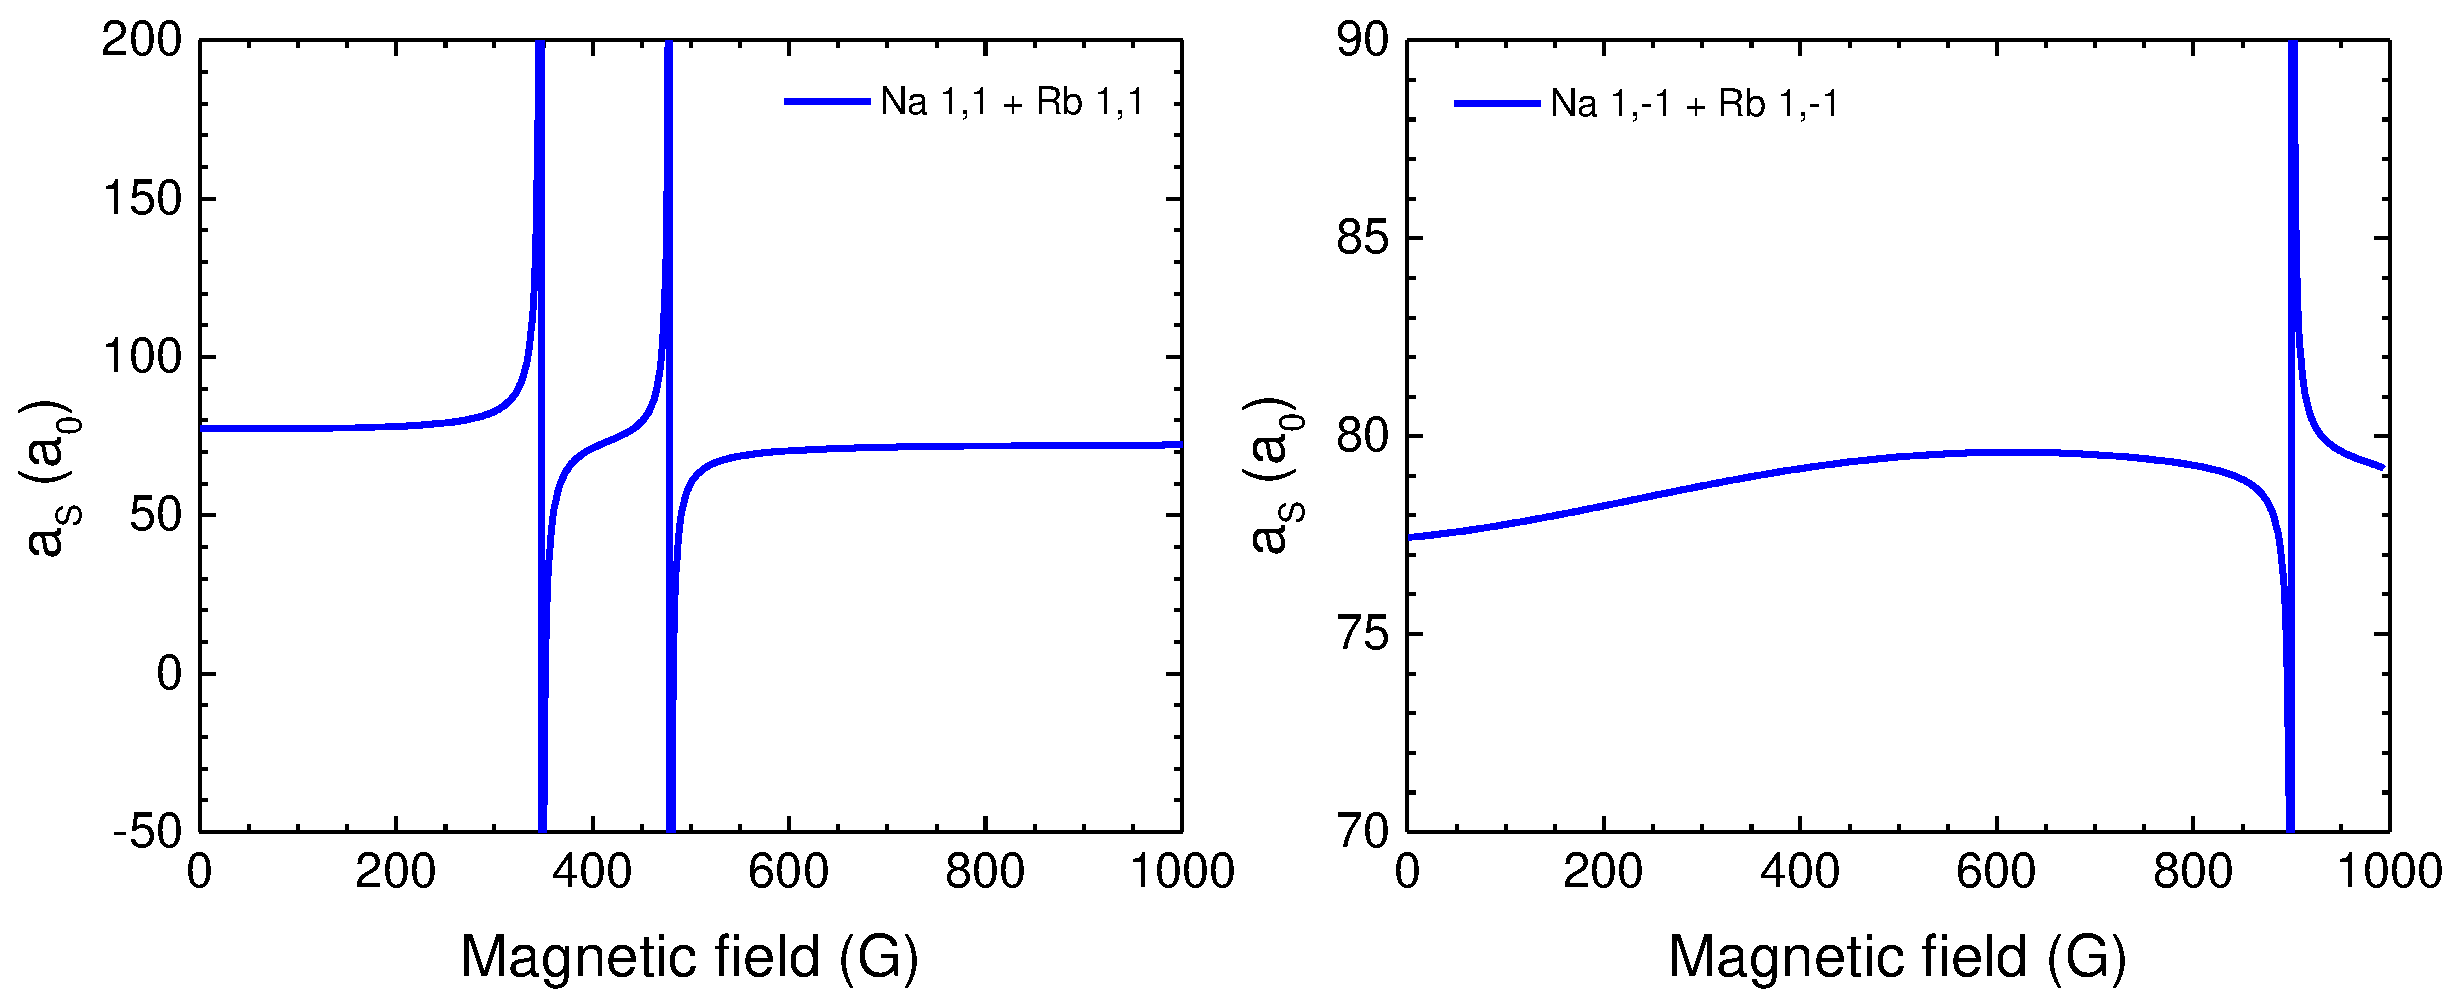
\includegraphics[width = \linewidth]{FR_groupAE.pdf}
\end{center}
\caption[Scattering lengths of Na$\ket{1}$+Rb$\ket{1}$ and Na$\ket{-1}$+Rb$\ket{-1}$ elastic channels]{Both Na$\ket{1}$+Rb$\ket{1}$ and Na$\ket{-1}$+Rb$\ket{-1}$ are elastic channels. Here we only plot the real part of the scattering length since there is no imaginary part. Two resonances show in Na$\ket{1}$+Rb$\ket{1}$ channel and one in Na$\ket{-1}$+Rb$\ket{-1}$ channel. A smooth variation of the scattering length is obvious in Na$\ket{-1}$+Rb$\ket{-1}$ channel.}
\label{FR_groupAE}
\end{figure}

% about elastic channel (done 2021-8-23 14:57:59)
As shown in Table~\ref{fst} and in Fig. \ref{FR_groupAE}, Na$\ket{1}$+Rb$\ket{1}$ Na$\ket{-1}$+Rb$\ket{-1}$ are two channels with all resonances elastic, which means there is no possible for the scattering to other channels. These resonances are a pole as shown in the scattering length plot following the $1/(B-B_0)$ variation. If only considering the two-body collision, one would not have the loss peak as shown in Fig. \ref{FR_loss} or Fig. \ref{FR_more}, because increasing the scattering length only means increasing the elastic collision rate. So, the loss peaks in those measurements are the result of the three-body loss.

% group B for total M=1 (done 2021-8-23 14:51:43)
\begin{figure}[htb]
\begin{center}
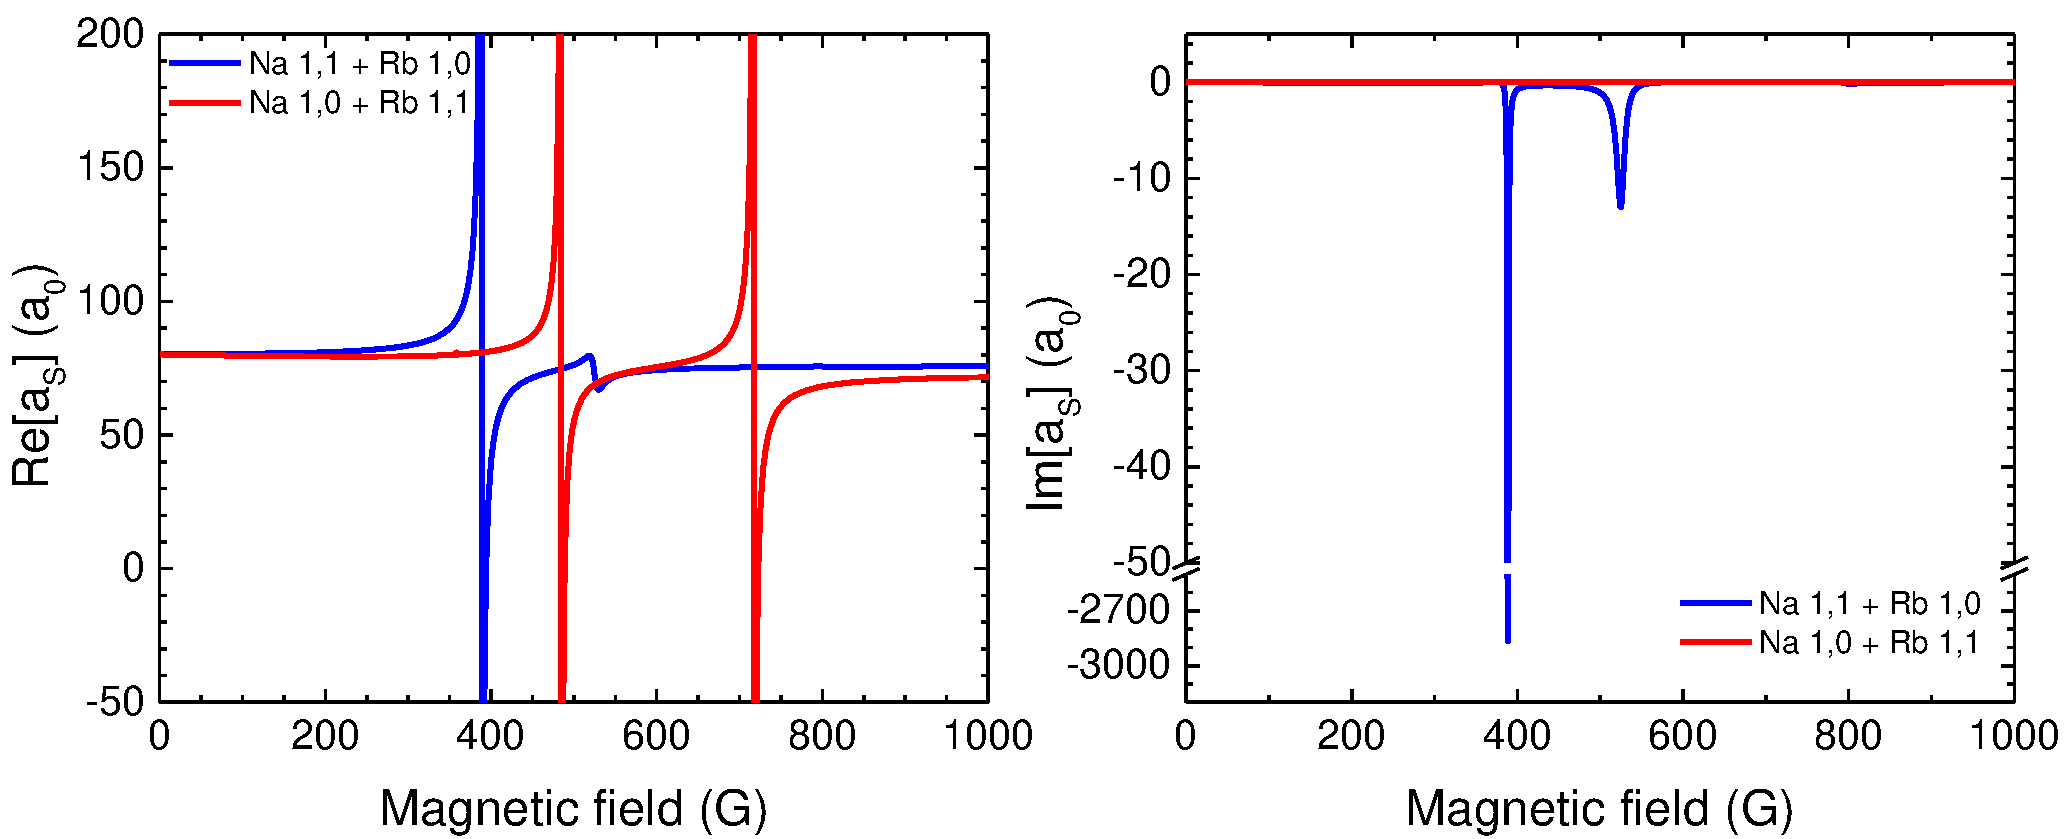
\includegraphics[width = \linewidth]{FR_groupB.pdf}
\end{center}
\caption[Scattering lengths of $M_F=1$ channels]{Scattering lengths of $M_F=1$ channels, including Na$\ket{1}$+Rb$\ket{0}$ and Na$\ket{0}$+Rb$\ket{1}$. Left(right) shows the real(imaginary) part of the scattering length. For Na$\ket{1}$+Rb$\ket{0}$ channel there are two inelastic resonance with non-zero imaginary part of scattering length.}
\label{FR_groupB}
\end{figure}
% group C for total M=0 (done 2021年8月24日12:12:39)
\begin{figure}[htb]
\begin{center}
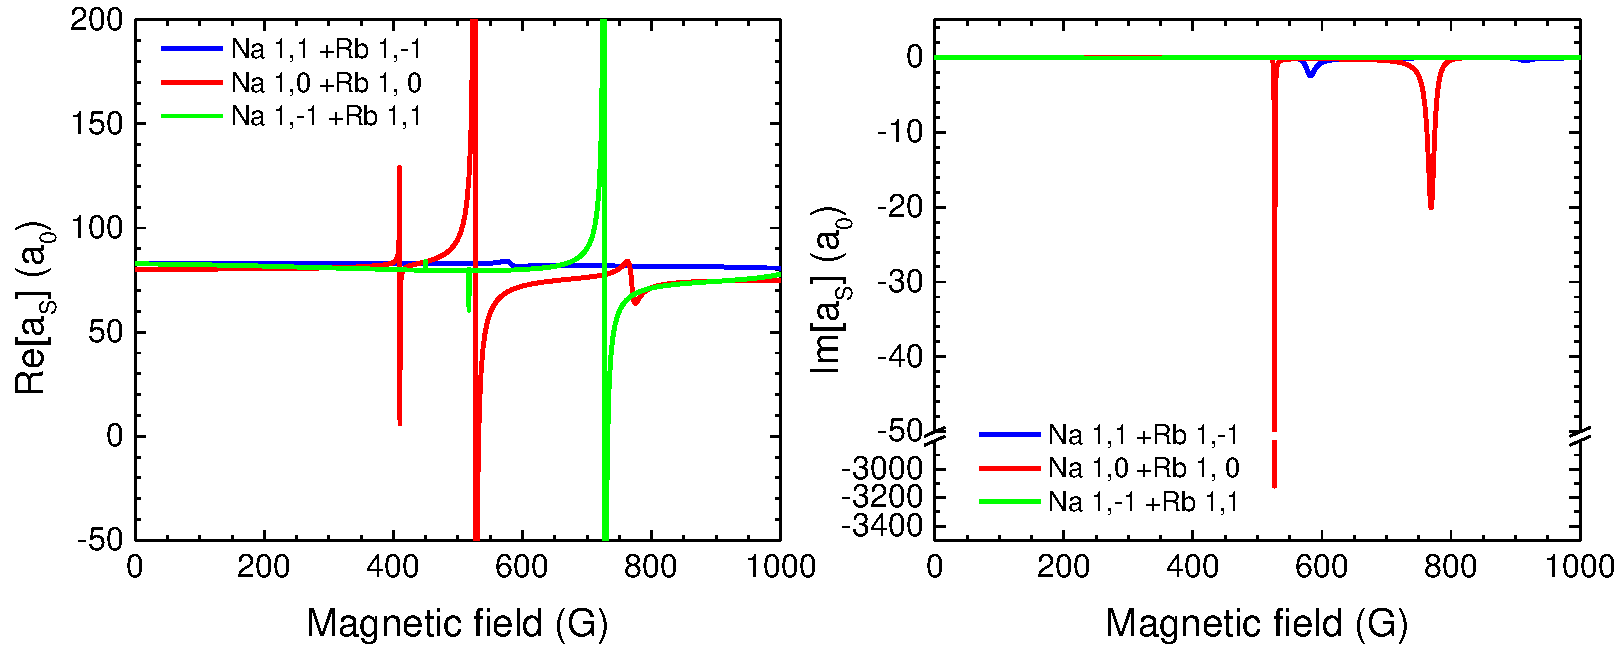
\includegraphics[width = \linewidth]{FR_groupC.pdf}
\end{center}
\caption[Scattering lengths of $M_F=0$ channels]{Scattering lengths of $M_F=0$ channels, including Na$\ket{1}$+Rb$\ket{-1}$, Na$\ket{0}$+Rb$\ket{0}$ and Na$\ket{-1}$+Rb$\ket{1}$. Left(right) shows the real(imaginary) part of the scattering length.}
\label{FR_groupC}
\end{figure}

% about inelastic channel I (done 2021年8月24日12:08:25)
When an inelastic channel is present, the states at the threshold are quasi-bound, so using FIELD is more complicated. Instead, the FRs are located by computing the scattering lengths for magnetic fields up to 1000 G using the MOLSCAT program~\cite{molscat:2019,mbf-github:2020}. Once an FR is located, the resonance parameters are then determined following the regularized scattering length or fully complex procedure of Ref.~\cite{Frye2017}. In this case, the scattering length is complex and shows an oscillation rather than a pole at resonance \cite{Hutson:res:2007}. Such a resonance is termed decayed, and the procedure generates the resonant scattering length $a_{\rm res}$ and the inelastic width $\Gamma_{\rm inel}$ in addition to $B_0^{\rm cc}$, $\Delta$ and $a_{\rm bg}$.

% about inelastic channel II (done 2021年8月24日12:09:06)
The calculation reproduces all the observed $s$-wave resonances. As shown in Table~\ref{fst}, the deviations between $B_0^{\rm cc}$ and $B_0^{\rm exp}$ are within 0.5 G for most of the elastic FRs, labelled by ``N'' in the last column ``inel?''. The only exception is the resonance observed at 410.9 G for the entrance channel $\ket{0} + \ket{0}$, for which $B_0^{\rm cc}$ is 1.1 G lower. As shown in Fig.~\ref{FR_Zeeman-BC}(b), this channel features a nearby switchover between the relative channel energies near 450 G. The four $s$-wave resonances for the entrance channels $\ket{1}+\ket{1}$ and $\ket{0}+ \ket{1}$ all have calculated resonance widths $\Delta$ of several Gauss. They should all be useful for investigating Na--Rb mixtures with tunable interactions. These resonances also have rather small calculated effective ranges, on the order of 10s of $a_0$; thus, using the scattering lengths should be sufficient for most applications.

% Zeeman energy for $M_F=1$ and $M_F=0$ channels (done 2021-8-23 10:26:28)
\begin{figure}[htb]
\begin{center}
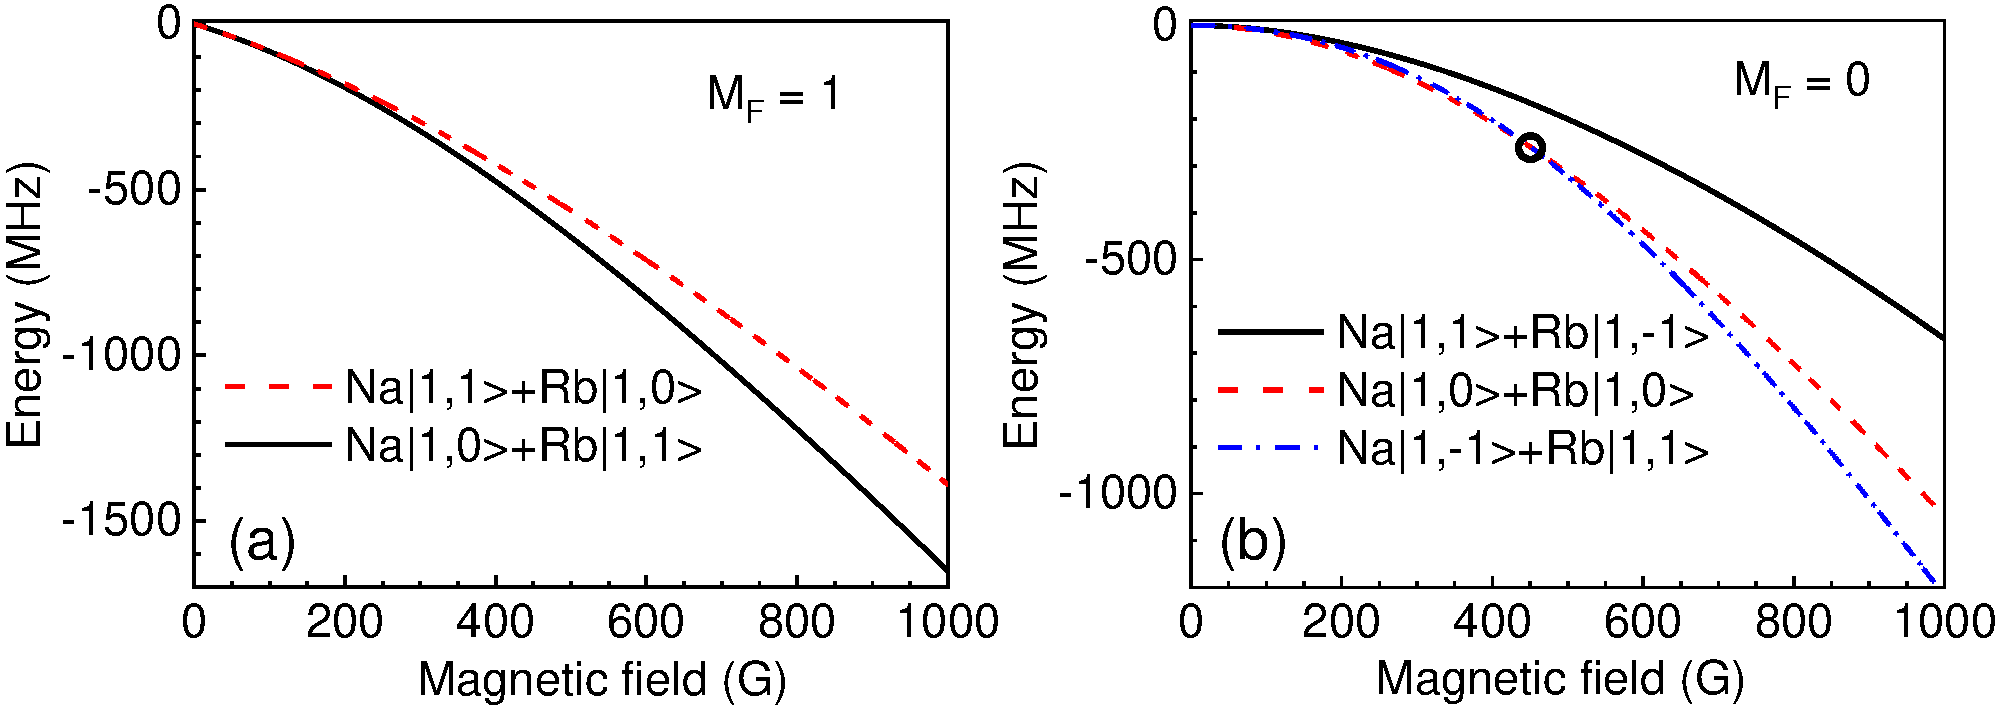
\includegraphics[width = \linewidth]{FR_Zeeman-BC.pdf}
\end{center}
\caption[Zeeman energy for $M_F=1$ and $M_F=0$ channels]{(a) Channel energies for the manifold with $M_F = 1$ for magnetic field up to 1000 G. (b) The same for the manifold with $M_F = 0$. The energies of the channels $\ket{0}+\ket{0}$ and $\ket{-1}+\ket{1}$ cross each other near 450 G, as marked by the black open circle. For each $M_F$, atom pairs in higher-energy channels can undergo inelastic loss by spin exchange to the lower-energy channels.}
\label{FR_Zeeman-BC}
\end{figure}

% about inelastic channel III (done 2021-8-24 12:09:25)
The decayed FRs can have very different characters, depending on $a_\textrm{res}$ and/or $\Gamma_\textrm{inel}$. When $a_\textrm{res}$ is large and $\Gamma_\textrm{inel}\ll\Delta$, the resonance \emph{may} be fairly similar to the elastic case and be dominated by three-body loss. However, when $a_\textrm{res}$ is small and $\Gamma_\textrm{inel}$ is comparable to or larger than $\Delta$, the loss is more likely to be dominated by two-body loss. This looks to be the case for the resonances at 522 G for $\ket{1}+\ket{0}$, at 759 G for $\ket{0}+\ket{0}$, and the unobserved one at 420 G for $\ket{-1}+\ket{1}$. It is also true for both resonances for $\ket{1}+\ket{-1}$, but for those there is a significant \emph{background} loss characterized by the imaginary part of $a_\textrm{bg}$.

% group D for total M=-1 (done 2021年8月24日12:12:28)
\begin{figure}[htb]
\begin{center}
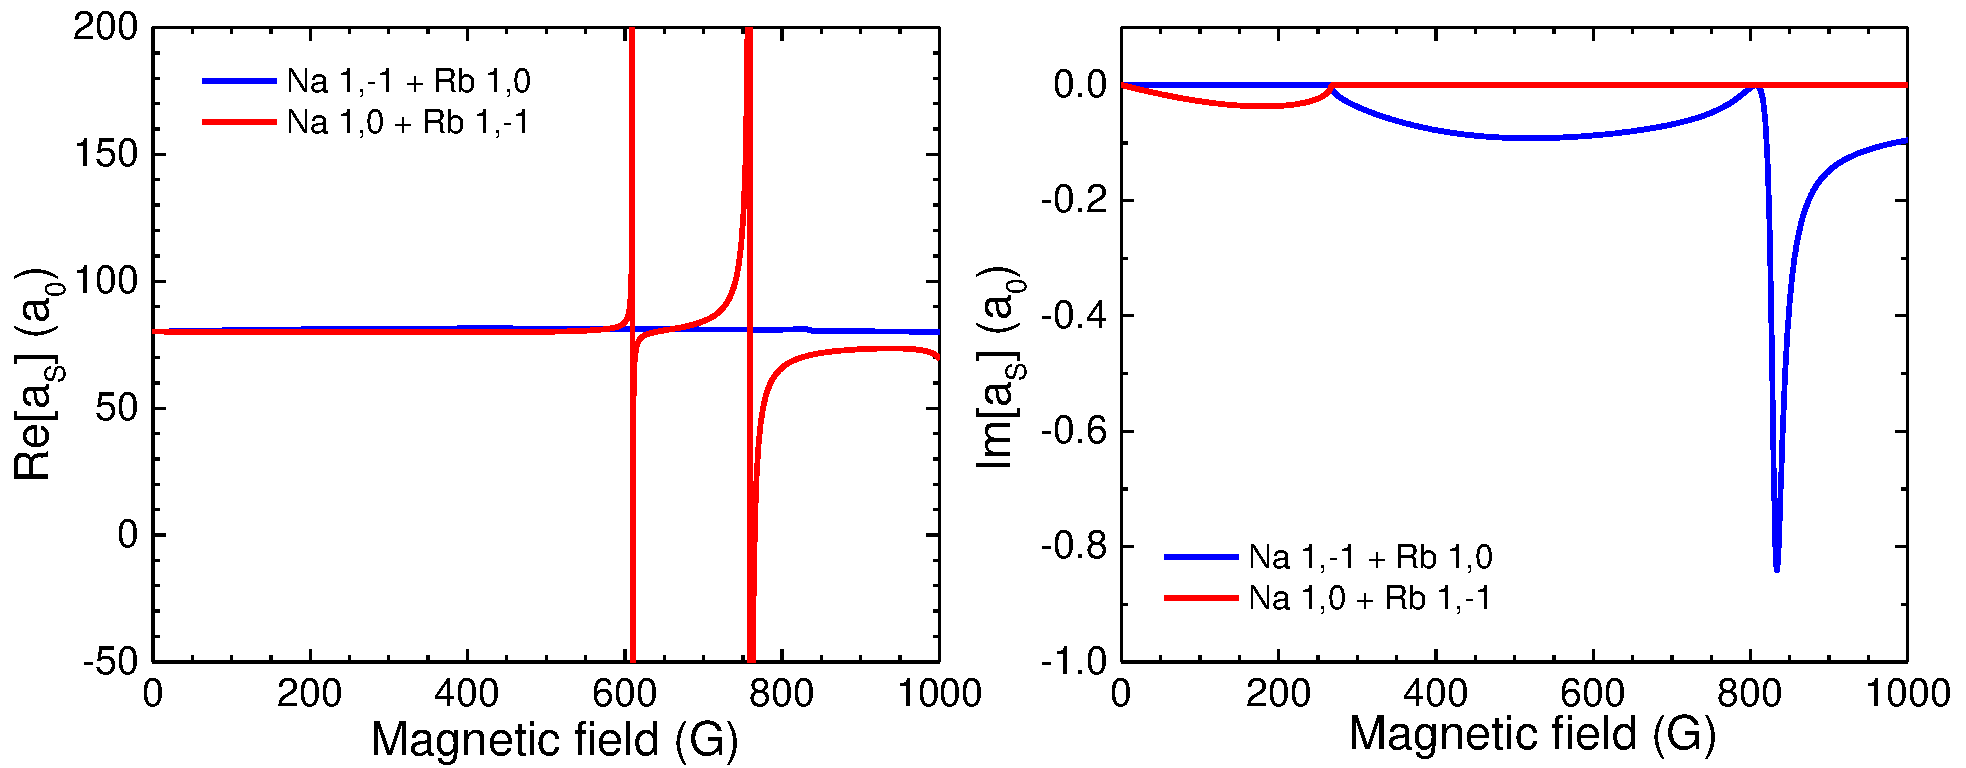
\includegraphics[width = \linewidth]{FR_groupD.pdf}
\end{center}
\caption[Scattering lengths of $M_F=-1$ channels]{Scattering lengths of $M_F=-1$ channels, including Na$\ket{0}$+Rb$\ket{-1}$ and Na$\ket{-1}$+Rb$\ket{0}$. Left(right) shows the real(imaginary) part of the scattering length.}
\label{FR_groupD}
\end{figure}

% about inelastic channel IV
For the decayed resonances with $\Gamma_\textrm{inel} <1$ at 388 G for $\ket{1}+\ket{0}$ and at 526 G for $\ket{0}+\ket{0}$, the calculated resonance positions $B_0^{\rm cc}$ agree with the measured resonance positions $B_0^{\rm exp}$ very well. However, deviations up to several Gauss are observed for inelastic resonances with large $\Gamma_\textrm{inel}$. These can be attributed to several factors. For the two resonances with very broad observed loss spectra at 522 G for $\ket{1}+\ket{0}$ and at 759 G for $\ket{0}+\ket{0}$, the resonance centers have large uncertainties near 10 G. In addition, in presence of the background loss, the two-body loss induced by these resonances has an asymmetric (Fano-like) profile and its measured peak is not at $B_0$. Finally, although we have not studied them carefully, some nearby intraspecies FRs in Na or Rb may also affect the measurements of the resonance positions.

% about those not observed
Several resonances predicted by the coupled-channel calculation are not observed experimentally. Most of these are very narrow ones with calculated $\Delta$ in the mG range. No resonance is found from the calculation for the entrance channel $\ket{0}+\ket{-1}$. In addition, we have not searched experimentally for FRs in the entrance channel $\ket{-1}+\ket{0}$ although the calculation indicates that two resonances should exist.

% about p-wave resonances and some comments
Table~\ref{fst} also lists the several $p$-wave FRs observed by~\cite{wang2013observation} for the entrance channels $\ket{1}+\ket{1}$ and $\ket{-1}+\ket{-1}$. As mentioned above, we have not attempted to improve the agreement between the current calculation and the experiment by including the dependence of the atomic hyperfine coupling on $R$. We note that Ref.~\cite{Cui2018}, which presented a compilation of FRs for alkali atoms calculated with multichannel quantum defect theory (MQDT), identified the resonance near 284 G as a ``broad'' $p$-wave resonance. It would be possible to perform a full-scale coupled-channel fitting to these resonances. This, however, is not pursued here as it would involve further adjustments to the potential parameters, beyond those used in Ref.\cite{guo2021leehuangyang}. In view of the inaccuracy of the loss spectroscopy compared with the measurements of FM binding energies, we believe such fitting is not currently justified.

\subsection{Na-Na and Rb-Rb scattering length}

% calculation
Besides interspecies Na-Rb scattering properties, we also study the intraspecies scattering length for Na-Na and Rb-Rb, because the droplet experiment needs all three scattering lengths. Out calculation directly send the potential file from \cite{} to MOLSCAT \cite{} and then use the molscat modular to obtain the scattering length. The Feshbach resonances for Na-Na and Rb-Rb are all far away from 347 G, where we study the droplet \cite{}. However, Na-Na scattering length varies with magnetic field very smoothly, even without resonance. As shown in Fig. \ref{FR_NaNa}, From 0 to around 800 G, we have a scattering length changing from 54.5 $a_0$ to about 64 $a_0$. For magnetic field around 350 G, i.e. the field for forming droplet sample, the scattering length for Na-Na is 60.05 $a_0$. This value is about 10\% larger than in a low magnetic field. 

% Na-Na 1,1 scattering length (done 2021-8-23 14:44:27)
\begin{figure}[htb]
\begin{center}
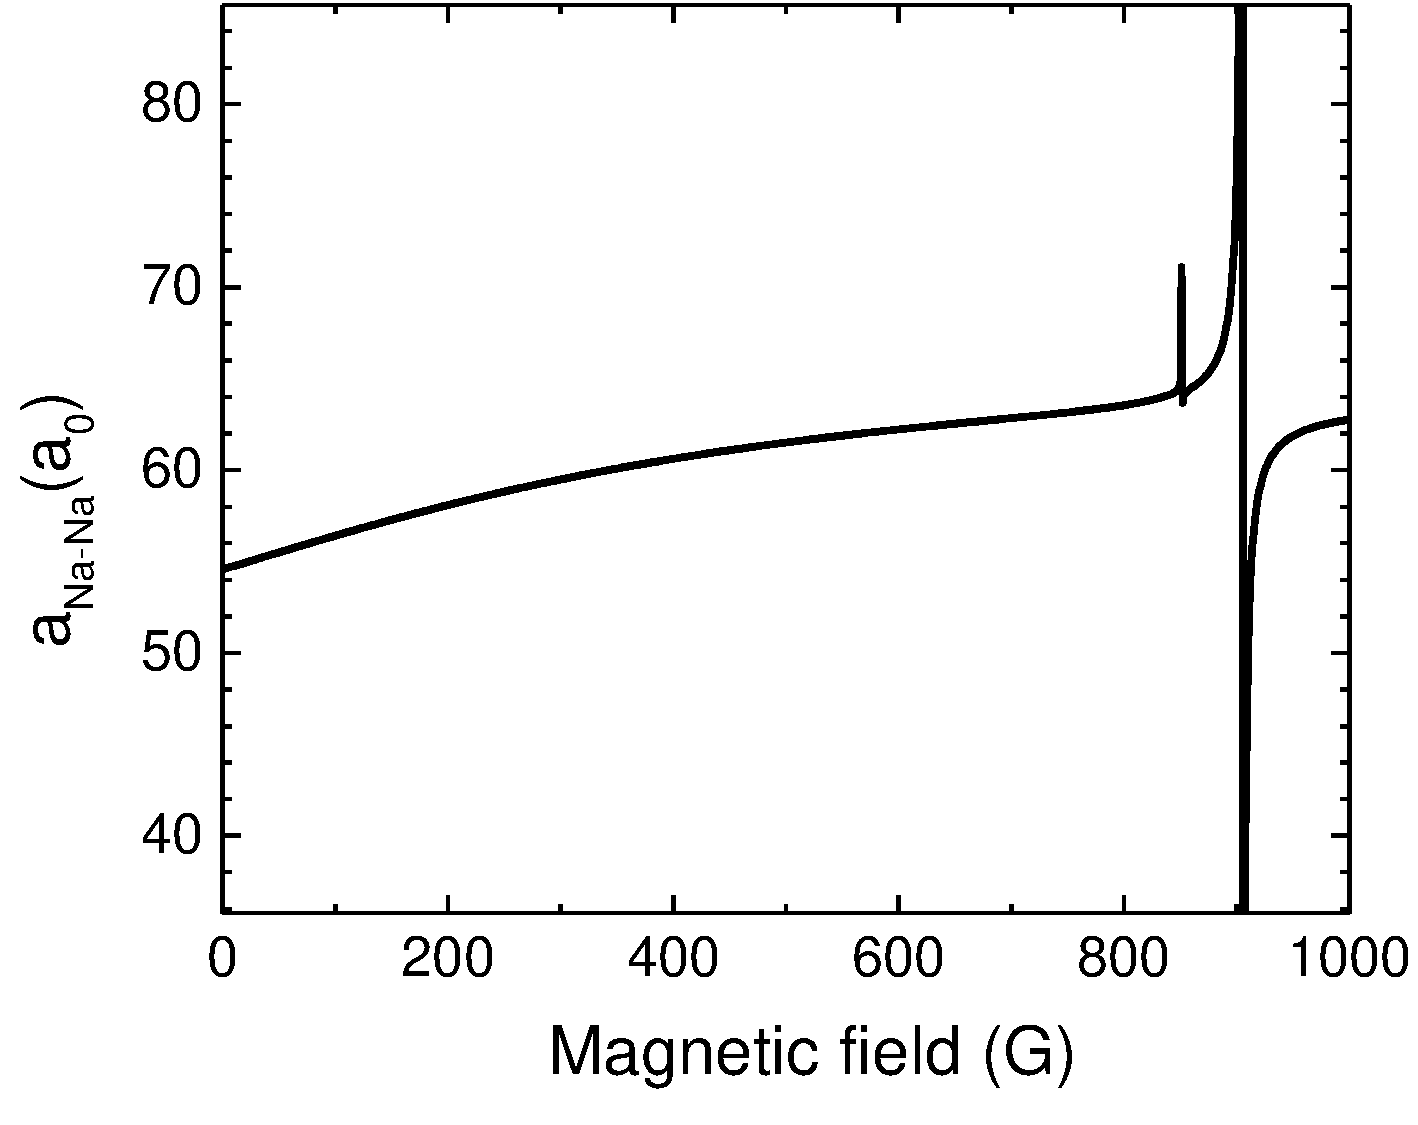
\includegraphics[width = 0.7\linewidth]{FR_NaNa.pdf}
\end{center}
\caption[Na$\ket{1,1}$ + Na$\ket{1,1}$ scattering length as a function of magnetic field]{Na$\ket{1,1}$ + Na$\ket{1,1}$ scattering length as a function of magnetic field. A smooth changing from }
\label{FR_NaNa}
\end{figure}

% more comments
Verifying the Na-Na scattering length value is not easy since the smooth-changing background scattering length only has about 10\% to 20\% variation. Typical methods for measuring $s$-wave scattering length, such as measurement of elastic collision rate by tracing the thermalization process\cite{} or by measuring the BEC expansion\cite{}, are all difficult and need precisely calibration of some other physical parameter (such as atomic number in the second method). These measurements are prone to have an error with 10\% to 20\%. On the other hand, the coupled-channel calculation is the most precise method and is an ab initio calculation that offers reliable numbers. So, we directly take the calculated one.

\chapterend
\chapter{Quantum droplet of hetero-nuclear Bose mixture}
\label{Chap_droplet}

% epigraph (done 2021-9-30 09:06:25)
\setlength{\unitlength}{1pt}
\setlength{\epigraphwidth}{10cm}
\epigraph{Law of physicists I: \\ Without experimentalists, theorists tend to drift. \cite{Lee:1992ui}}{--- T.D. Lee\\ \textit{History of the weak interactions (1987)}}

% 历史在这里讲

% Overview and structure of theory part of this chapter (done 2021-10-7 20:49:40)
This chapter discusses the heteronuclear droplets formed by the Bose-Einstein condensate mixture of Na and Rb. We first re-analyze the droplet, however, with a finite volume instead of homogeneous density distribution. This is to compare with experiments since an actual quantum droplet we build in the experiment always has a specific size due to a limited atomic number. We make a rough estimation by analyzing the energy scales of each term. Then, continuing with the analytical solution in Sec. \ref{sec:droplet_ana}, we implement the variational calculation. We use a simple Gaussian trial function to help understand how different energy scales compete in the finite-size droplets. Its specific size mainly requires introducing a kinetic energy term (i.e. quantum pressure). In order to better understand the droplet sample, we simulate it with extended Gross–Pitaevskii equation (eGPE). In this part, we give the derivation of the extended GPE especially for the two-species BEC sample near zero MF energy region.

% Overview and structure of experiment part of this chapter (done 2021-10-7 22:54:47)
In Sec. \ref{sec:droplet_experiment}, we experimentally study Na-Rb droplet and measure the phase diagram of liquid-gas phase transition, which is the central part of our experimental research. The experimental method is simple and straightforward. We directly let the sample do Time-of-Flight and observe the non-expansion signal. This method avoids the complexity of the optical-levitation method however need more effort to eliminate the inhomogeneity of the magnetic field. In order to cooperate with this scheme, we upgrade our system on both control of magnetic field and imaging method, referring to Sec. \ref{sec:image} and Sec. \ref{sec:fastcoil} for details. Later, in Sec. \ref{sec:LHY_gas}, we study the gaseous LHY sample. This research aims to explore the behaviour of a gaseous sample under the dominance of LHY energy instead of MF energy. This research is a supplement to the study of LHY gas by measuring the trap frequency \cite{skov2020}. After understanding the droplet formation process, we realize that the previous process of preparing droplets is far from adiabatic, which resulted in significant limitations on the sample life and the number of atoms. So we improve the preparation scheme to achieve a droplet sample with more numbers as shown in Sec. \ref{sec:mode_match}. 
%Finally, Sec. \ref{sec:droplet_molecule} shows our efforts on using droplets to form the Feshbach molecules. Although the conversion efficiency has no improvement, we have greatly reduced the temperature of the molecules and provide a promising path for the future production of degenerate Feshbach molecules.


\section{Quantum droplet with finite size}
\label{sec:finite_size}

% overall of this section (done 2021-10-8 09:20:57)
In Sec. \ref{sec:droplet_ana}, we calculate the quantum liquid analytically, showing the mean-field and LHY energy expressions. Then we obtain the equilibrium density of the system. This calculation ignores the system's quantum pressure (kinetic energy), which means it is only proper for homogeneous bulk samples. However, in our experiments, due to the limitation of the atomic number, we currently cannot obtain a sample with a large enough number allowing us to ignore its edge. Thus, in this section, we first analyse the quantum pressure caused by the finite volume then show its influence on the quantum liquid droplet. 

% introducing energy expression (done 2021-10-14 23:14:55)
The total energy of the system consists of three parts; in addition to the interaction energy (Mean-field energy and LHY correction), there is also the quantum pressure due to the finite size of the sample. This can also be explained by the uncertainty principle since the finite size can be viewed as a size limitation and will introduce a finite momentum (energy). The total energy expression of this finite-size droplet sample is
\begin{equation}
\begin{split}
E_{\text{total}}&=E_{\text{kin}}+E_{\text{MF}}+E_{\text{LHY}}\\
E_{\text{kin}}&=N \frac{\hbar ^2}{2m}\int \left| \nabla \phi (\pmb{r})\right| ^2 \, dr^3\\
E_{\text{MF}}&=\frac{g}{2}N^2\int \left| \phi (\pmb{r})\right| ^4 \, dr^3,\quad g=\frac{2\pi  \hbar ^2a_S}{m/2}
\end{split}
\end{equation}
where $N$ is particle number, $m$ is its mass, $g$ is the interaction strength which is proportional to scattering length $a_S$. Note that here we write down the formula with only single species, however later we need to extend it to double species case, which is just summation along two species for all $N$ and $g_{ij}$. The LHY correction expression needs an infinite integration which is will be explained later.

% explain three terms (done 2021-10-22 11:46:21)
Locally, MF energy is proportional to $n^2$, and LHY correction is proportional to $n^{5/2}$. The kinetic energy (quantum pressure) is proportional to the square of the derivation of the wave function. For a homogeneous bulk sample, just as we mentioned in Chap. \ref{Chap:theory}, the quantum pressure term is zero. However, considering a finite size sample, the rapid decreasing of the wave function on the boundary (the density inside is limited and the outside is the vacuum) introduces additional kinetic energy. This kinetic energy tends to reduce the variation rate of the wave function (density) on the boundary. So it tends to inflate the sample. This term does not exist in a classic system but only in a quantum system which is the same as the LHY term. 

% surface tension and core pressure (done 2021-10-22 11:47)
Another phenomenon called surface tension can be explained by MF energy on the boundary. At the boundary, density is lower than at the core part, and the positive energy of LHY is much smaller than the attraction energy of MF. So the attraction force is dominated by MF energy and offer surface tension similar to the classical liquid. From another perspective, MF energy is a zero-order approximation, both existing in classical and quantum systems. This surface tension will cause the pressure at the core to be higher than the homogeneous sample. In the finite droplet case, because the environment is with zero pressure, thus the core of the sample will have a pressure higher than zero. This can be offered by the LHY term, as we mentioned in Chap. \ref{Chap:theory}, the LHY term increase faster than the MF term with increasing density. So, the LHY repulsion overcomes the MF attraction at the core and support the sample without collapsing.

% droplet density distribution (done 2021-10-22 12:24:37)
\begin{figure}[htb]
\begin{center}
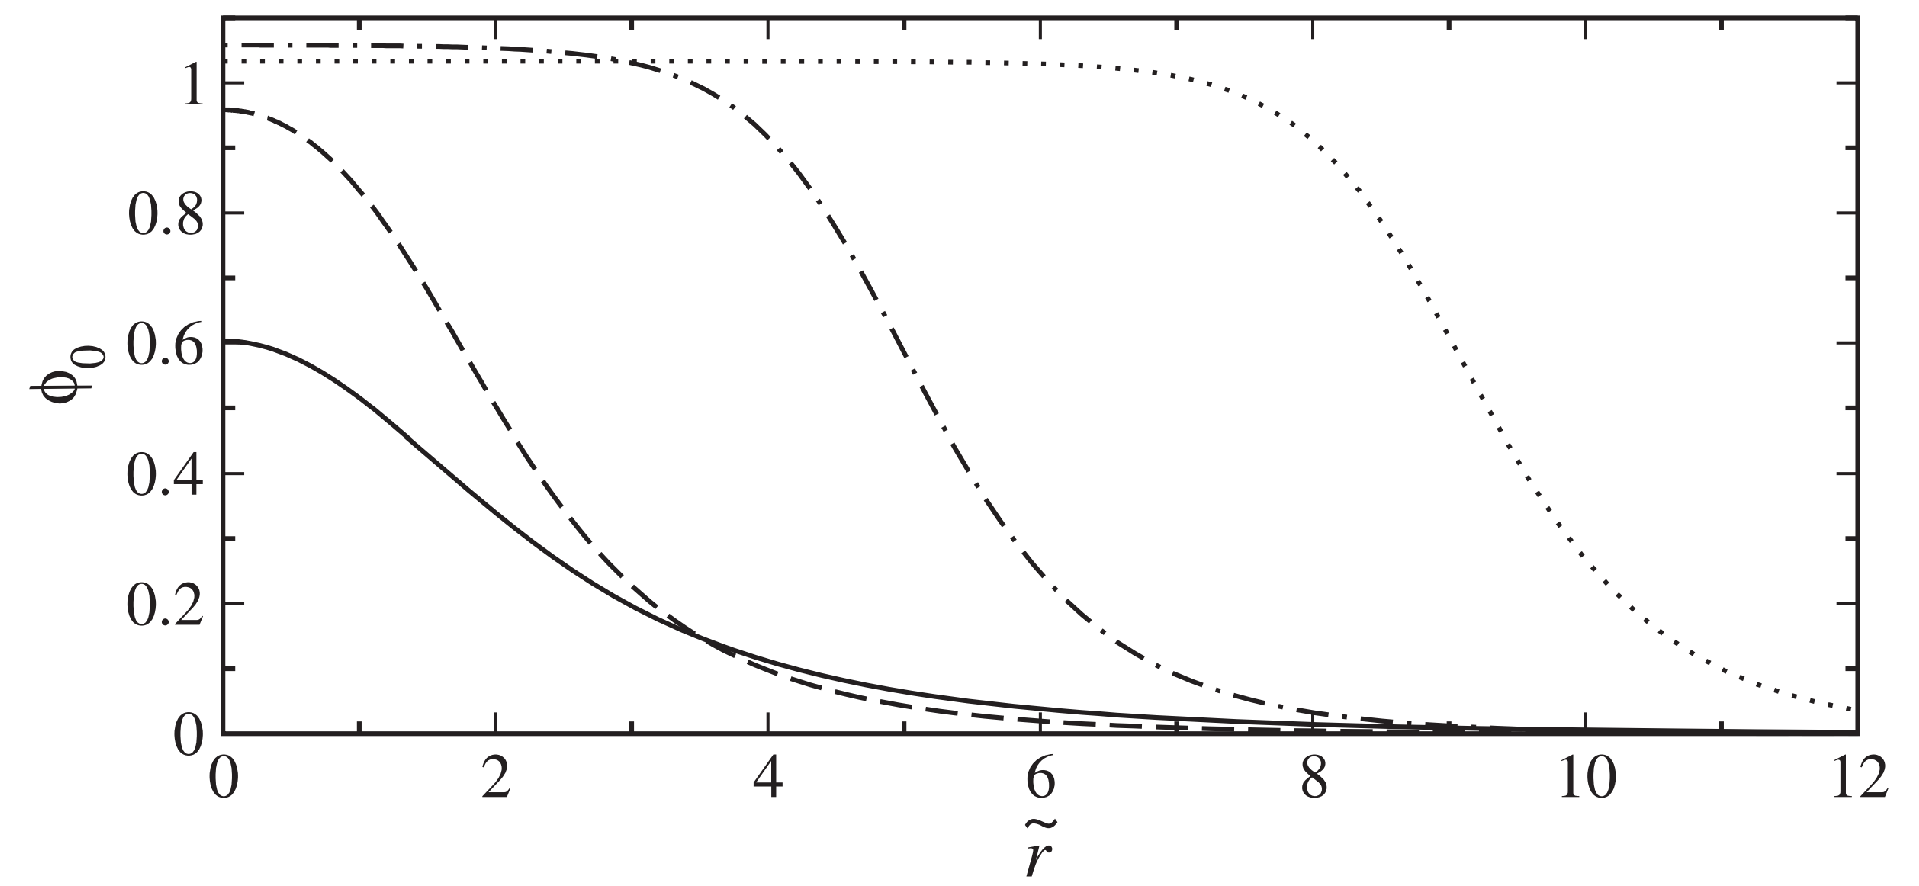
\includegraphics[width = 0.8\linewidth]{droplet_density_dis.pdf}
\end{center}
\caption[Droplet density distribution and edge effect]{Figure shows the density distribution of a finite-size droplet. The edge size is of about one $\hat{r}$ which provides the surface tension. Figure from \cite{petrov2015}.}
\label{droplet_density_dis}
\end{figure}

% quantum droplet with trap (done 2021-10-22 12:11:21)
In addition to the quantum droplet of free space, we also discuss the sample of in trap. For the in-trap sample, we need to add an additional energy term of the trap. So, the total energy is made of four parts now. For a sample with finite size, trap energy and quantum pressure behaves opposite. Small size introduces higher quantum pressure but reduces trap energy and vice versa. This is similar for MF and LHY energy, where MF energy is negative; however, LHY energy is positive. For samples with specific sizes, these two-term compete with each other. Analyzing such a sample with two groups of energies competing with each other is not straightforward. Therefore, the calculation of the variational method we introduced in Sec. \ref{sec:var_cal} can help us understand better. This part is explained carefully in sec. For more detailed calculations, please refer to \cite{Liu2020}.

\section{Variational calculation}
\label{sec:var_cal}

% overall of this section (done 2021-10-14 23:28:26)
In this section, we introduce the variational calculation of droplets. Variational calculations can help us better understand the energy competition in the system. From the analysis in the previous section, we can read that whatever the quantum pressure or the interaction energy in a quantum droplet of finite volume,  they all depend on the system's wave function distribution. Thus, a pure analytical calculation lacks information and can not reveal how these different energies compete with each other.

% why we use variational method instead of directly using GPE simulation (done 2021-10-14 23:47:19)
A more accurate method is the finite element method, which treats the entire wave function as a function of space coordinates. Then it uses a variational method to adjust the value of the wave function at each spatial position, reducing the overall system's energy, thereby providing a more accurate solution. However, the calculation of the three-dimensional system consumes vast computing resources, which is incapable of ordinary personal computers. In order to understand the behaviour of the system, we need an intermediate model to help us establish the relationship between various causes and effects. After this step, the subsequent GPE simulation will be more straightforward.

% section structure (done 2021-10-29 20:56:48)
This section first reviews the variational calculation of single species BEC and defines the so-called release energy. We explain how release energy reflects the interaction and the measurement of the second-order correlation function. At the same time, this also gives an experimental measurement method, i.e. the direct TOF method. Then we show the introduction of the Gaussian variational method in the double-species system. Although it is a very rough approximation, the calculation should be pretty effective for the case with a relatively small atomic number and the droplet sample far away from the top-flat density distribution at the centre. This will be verified in subsequent calculations. We imitate the dimensionless parameters of the single-species BEC and introduce two dimensionless parameters to characterize the double-species BEC in the trap. Thereby it is convenient to describe the system and compare it with different species combinations.

% more details (done 2021-10-29 21:03:11)
We calculate two items by the variational method: 1. LHY gas in a harmonic trap and the released energy when expansion in free-space. 2. Droplet with magnetic field gradient and how the critical number is shifting. We start from a single BEC in a harmonic trap and review the variational method with Gaussian Ansatz. Noted that, we get the $\chi $= - 0.67 there is a collapse point, which offers no solution. Then, we plot the release energy curve. The release energy is just the sum of kinetic energy in the trap plus the interaction energy. For the Double BEC near-zero MF energy, the behaviour of the sample is very similar to a single BEC, as the $\lambda_+$ branch requires minimum density, leaving only the $\lambda_-$ branch. So, assuming that Na and Rb share the same wave function, we can use the result from the single BEC part. By choosing the correct characteristic value, we can make a comparison for experimental data.

% GPE vs. variational method (done 2021-10-29 21:05:50)
We also use the eGPE to calculate the release energy in Sec. \ref{sec:eGPE}, due to Gaussian Ansatz does not fit for large atomic number cases. We find a great overlap between our experiment and the eGPE simulation. In comparing the MF and LHY cases, we can say that we measured the LHY energy for the zero-MF with a shift from 0.75$\hbar \omega $ to about 1.3 $\hbar\omega$. This relatively large shift is definite beyond MF theory. The eGPE simulation cannot give out physics explanation. However, the variational method can. So, we plot all kinds of energy as a function of the variational parameter $w$. This plot can explain several questions: 1. How do these different energies compete? What is the meaning of the meta-stable state of a droplet? 2. What parameter do we need to characterize the LHY term? Moreover, how large is this term compared to the MF term and others? 3. what will happen if the initial state does not match the droplet state? Will the expansion over the local maximum and miss the droplet formation?

% more(done 2021-10-29 21:06:08)
Finally, we add one more variational parameter to the Gaussian Ansatz to explain the shift of critical numbers when the magnetic field gradient exists. The main idea is that Na and Rb wavefunction will surfer a tiny centre shifting $\delta $, which decrease the absolute value of Mean-Field energy between Na and Rb. Because the $E_{\text{MF$\_$Rb}-\text{Na}}$ is the product of their density. So the overlap will change dramatically. However, The rest part of MF and LHY energy will keep. So, this gradient will decrease the binding term when we are in the droplet region, which shifts the critical number above.

\subsection{Single species BEC in harmonic trap}

% Hamiltonian and energy (done 2021-10-16 06:58:29)
We first recall the textbook result of the variational solution about a single BEC in harmonic trap. Here, we introduce the Gaussian ansatz as an approximation. Considering N Bosons in a harmonic trap with trap frequency of $\omega _0$, its ground state energy is made of 
\begin{equation}
\begin{split}
E_{\text{kin}}&=N \frac{\hbar ^2}{2m}\int \left| \nabla \phi (\pmb{r})\right| ^2 \, dr^3\\
E_{\text{trap}}&=N\int \left| \phi (\pmb{r})\right| ^2V_{\text{trap}}(\pmb{r})dr^3,\text{   }V_{\text{trap}}(\pmb{r})=\frac{1}{2}m \omega _0^2\pmb{r}^2\\
E_{\text{MF}}&=\frac{g}{2}N^2\int \left| \phi (\pmb{r})\right| ^4 \, dr^3,\quad g=\frac{2\pi  \hbar ^2a_S}{m/2}
\end{split}
\end{equation}
where we for now ignore the LHY correction. For convenience we define the harmonic length $a_{\text{ho}}=\sqrt{\frac{\hbar }{m \omega _0}}$.

% Gaussian ansatz and variational energy (done 2021-10-16 07:03:10)
Now, we use variational method to calculate the wave-function in trap. the Gaussian ansatz is 
\begin{equation}
\phi (\pmb{r})=\frac{1}{\pi^{3/4}\left(w^3a_{\text{ho}}^3\right){}^{1/2}}e^{-\frac{\pmb{r}^2}{2w^2a_{\text{ho}}^2}}
\end{equation}
where the $w$ is the variational parameter. Then, we have
\begin{equation}
\begin{split}
E_{\text{kin}}&=N \frac{\hbar^2}{2m}\int \left|\nabla\phi(\pmb{r})\right|^2 dr^3=N\hbar\omega_0\frac{3}{4w^2}\\
E_{\text{trap}}&=N\int\left|\phi(\pmb{r})\right| ^2 V_{\text{trap}}(\pmb{r})dr^3 = N\hbar\omega_0\left(\frac{3}{4} w^2\right)\\
E_{\text{MF}}&=\frac{g}{2}N^2\int\left|\phi(\pmb{r})\right|^4dr^3=N \hbar\omega_0\left(\frac{1}{\sqrt{2\pi}}\frac{a_SN}{a_{\text{ho}}}\frac{1}{w^3}\right)
\end{split}
\end{equation}
i.e. total energy 
\begin{equation}
E_{\text{tot}}(w)=N\hbar\omega_0\left(\frac{3}{4}\frac{1}{w^2}+\frac{3}{4}w^2+\frac{1}{\sqrt{2\pi}}\frac{a_SN}{a_{\text{ho}}}\frac{1}{w^3}\right)
\end{equation}

% minimize energy to get ground state (done 2021-10-16 07:03:00)
Then we minimize the $E_{\text{tot} }$ with the constrain of $\int\phi\phi^*dr^3=N$
\begin{equation}
E_{\text{tot}}(w)-\mu N=N \hbar  \omega _0\left(\frac{3}{4}\frac{1}{w^2}+\frac{3}{4}w^2+\frac{1}{\sqrt{2\pi }}\frac{a_SN}{a_{\text{ho}}}\frac{1}{w^3}\right)-\mu  N
\end{equation}
To get the $w$ of ground state, we take the derivative of $E_{\text{tot}}$
\begin{equation}
{\partial _w\left(\frac{3}{4}\frac{1}{w^2}+\frac{3}{4}w^2+\frac{1}{\sqrt{2\pi }}\frac{\chi }{w^3}\right)}=-\frac{3}{2 w^3}+\frac{3 w}{2}-\frac{3 \chi }{\sqrt{2 \pi } w^4}
\end{equation}
where we use $\chi $ represent the dimensionless quantity $\frac{a_SN}{a_{\text{ho}}}$.

\begin{itemize}[noitemsep,topsep=0pt]
    \item If tuning $g=0$, i.e. the non-interacting case, we get back to the single particle picture. The wave-function is a Gaussian with size of harmonic length, i.e. $w=1$
    \item With increasing $\chi $, we have larger size (larger $w$), and finally, when reach $\chi >>1$ limit, we turn to the Thomas-Fermi limit.
    \item For $\chi <0$, we have attractive Bose gas, with collapse point at $\chi =-0.671$ \cite{}
\end{itemize}

\subsection{Double BEC in harmonic trap with near zero-MF interaction}

% Hamiltonian and energy
Now we turn to our double species case, i.e. $N_{\text{Rb}}$ Rb and $N_{\text{Na}}$ Na in a harmonic trap with trap frequency of $\omega_{\text{Rb}}$ and $\omega _{\text{Na}}$, we have ground state energy of
\begin{equation}
\begin{split}
E_{\text{kin}}&=N_{\text{Na}}\frac{\hbar^2}{2m_{\text{Na}}}\int \left| \nabla \phi _{\text{Na}}(\pmb{r})\right|^2dr^3+N_{\text{Rb}}\frac{\hbar ^2}{2m_{\text{Rb}}}\int\left|\nabla\phi_{\text{Rb}}(\pmb{r})\right|^2dr^3\\
E_{\text{trap}}&=N_{\text{Na}}\int\left|\phi_{\text{Na}}(\pmb{r})\right|^2V_{\text{trap}-\text{Na}}(\pmb{r})dr^3+N_{\text{Rb}}\int\left|\phi _{\text{Rb}}(\pmb{r})\right|^2V_{\text{trap}-\text{Rb}}(\pmb{r})dr^3\\
E_{\text{MF}}&=\frac{g_{\text{Na}}}{2}N_{\text{Na}}^2\int\left|\phi_{\text{Na}}(\pmb{r})\right|^4dr^3+\frac{g_{\text{Rb}}}{2}N_{\text{Rb}}^2\int\left|\phi_{\text{Rb}}(\pmb{r})\right|^4dr^3\\
&\qquad\qquad\qquad\qquad+g_{\text{Rb},\text{Na}}N_{\text{Na}}N_{\text{Rb}}\int\left|\phi_{\text{Rb}}(\pmb{r})\right|^2\left|\phi_{\text{Na}}(\pmb{r})\right|^2dr^3\\
E_{\text{LHY}}&=\int\frac{256\sqrt{\pi}\hbar^2}{15}\left(m_{\text{Na}}^{-2/5}a_{\text{Na}}\left|\phi_{\text{Na}}(\pmb{r})\right|^2+m_{\text{Rb}}^{-2/5}a_{\text{Rb}}\left|\phi_{\text{Rb}}(\pmb{r})\right|^2\right)^{5/2}dr^3
\end{split}
\end{equation}
where
\begin{equation}
\begin{split}
&V_{\text{trap}-\text{Rb}}(\pmb{r})=\frac{1}{2}m_{\text{Rb}}\omega _{\text{Rb}}^2\pmb{r}^2,V_{\text{trap}-\text{Na}}(\pmb{r})=\frac{1}{2}m_{\text{Na}} \omega _{\text{Na}}^2\pmb{r}^2\\
g_{\text{Rb}}&=\frac{2\pi\hbar^2a_{\text{Rb}}}{\left.m_{\text{Rb}}\right/2},\text{}g_{\text{Na}}=\frac{2\pi\hbar^2a_{\text{Na}}}{\left.m_{\text{Na}}\right/2},\text{     }g_{\text{Rb},\text{Na}}=\frac{2\pi  \hbar ^2a_{\text{Rb},\text{Na}}}{m_{\text{Rb}}m_{\text{Na}}/\left(m_{\text{Rb}}+m_{\text{Na}}\right)}\\
\end{split}    
\end{equation}
As we are dealing with the case of $E_{\text{MF}}\to 0$, we can make several approximation:
\begin{itemize}[noitemsep,topsep=0pt]
    \item Two BECs share the same wave-function $\phi (\pmb{r})$
    \item Gaussian Ansatz
\end{itemize}
With the first approximation, we can rewrite the Hamiltonian as
\begin{equation*}
\begin{split}
E_{\text{kin}}&=\left(\frac{N_{\text{Na}}}{m_{\text{Na}}} +\frac{N_{\text{Rb}}}{m_{\text{Rb}}}\right)\frac{\hbar ^2}{2}\int \left| \nabla \phi (\pmb{r})\right|^2 dr^3=\frac{N}{m} \frac{\hbar ^2}{2}\int \left| \nabla \phi (\pmb{r})\right| ^2 \, dr^3\\
E_{\text{trap}}&=\frac{1}{2}\left(m_{\text{Rb}} \omega _{\text{Rb}}^2N_{\text{Rb}}+m_{\text{Na}} \omega _{\text{Na}}^2N_{\text{Na}}\right)\int \left|\phi (\pmb{r})\right| ^2\pmb{r}^2dr^3=\frac{1}{2}m \omega ^2N\int \left| \phi (\pmb{r})\right| ^2\pmb{r}^2dr^3\\
E_{\text{MF}}&=\frac{g_{\text{Na}}N_{\text{Na}}^2+g_{\text{Rb}}N_{\text{Rb}}^2+2g_{\text{Rb},\text{Na}}N_{\text{Na}}N_{\text{Rb}}}{2}\int \left| \phi(\pmb{r})\right| ^4 \, dr^3=\frac{g}{2}N^2\int \left| \phi (\pmb{r})\right| ^4 \, dr^3\\
E_{\text{LHY}}&=\frac{8\left(m_{\text{Na}}^{3/5}g_{\text{Na}}N_{\text{Na}}+m_{\text{Rb}}^{3/5}g_{\text{Rb}}N_{\text{Rb}}\right)^{5/2}}{15\pi ^2\hbar ^3}\int\left| \phi (\pmb{r})\right| ^5dr^3=\frac{8m^{3/2}\Gamma ^{5/2}N^{5/2}}{15\pi ^2\hbar ^3}\int \left| \phi (\pmb{r})\right| ^5 dr^3
\end{split}
\end{equation*}
Now, we recover to the single component case, with new mass, number, trap frequency and interaction strength following \pmb{ the negative branch} as shown in \cite{petrov2015}
\begin{equation}
E_{\text{MF}-}=\lambda _-n_-^2, \quad\text{with}\quad \lambda _-=\frac{\text{$\delta$g}\sqrt{g_{\text{Rb}}g_{\text{Na}}}}{\left(g_{\text{Na}}+g_{\text{Rb}}\right)}\quad\text{and}\quad n_-=\frac{n_{\text{Rb}}\sqrt{g_{\text{Na}}}+n_{\text{Na}}\sqrt{g_{\text{Rb}}}}{\sqrt{g_{\text{Na}}+g_{\text{Rb}}}}
\end{equation}
Thus, we can define the new number and interaction strength as
\begin{equation}
\begin{split}
N&=N_-=\frac{N_{\text{Rb}}\sqrt{g_{\text{Na}}}+N_{\text{Na}}\sqrt{g_{\text{Rb}}}}{\sqrt{g_{\text{Na}}+g_{\text{Rb}}}}\\
g&=\frac{4\pi  \hbar ^2a_S}{m}=2\lambda _-=\frac{2\text{$\delta $g}\sqrt{g_{\text{Rb}}g_{\text{Na}}}}{\left(g_{\text{Na}}+g_{\text{Rb}}\right)},\text{  }\text{$\delta $g}=g_{\text{Rb},\text{Na}}+\sqrt{g_{\text{Rb}}g_{\text{Na}}}
\end{split}
\end{equation}
Then, we have
\begin{equation}
\begin{split}
m&=\frac{N m_{\text{Na}}m_{\text{Rb}}}{N_{\text{Na}}m_{\text{Rb}}+N_{\text{Rb}}m_{\text{Na}}}\\
\omega&=\sqrt{\frac{\left(N_{\text{Na}}m_{\text{Rb}}+N_{\text{Rb}}m_{\text{Na}}\right)\left(m_{\text{Rb}}\omega_{\text{Rb}}^2N_{\text{Rb}}+m_{\text{Na}}\omega_{\text{Na}}^2N_{\text{Na}}\right)}{N^2m_{\text{Na}}m_{\text{Rb}}}}\\
\Gamma&=\frac{m_{\text{Na}}^{3/5}g_{\text{Na}}N_{\text{Na}}+m_{\text{Rb}}^{3/5}g_{\text{Rb}}N_{\text{Rb}}}{m^{3/5}N}=\frac{4\pi  \hbar ^2A}{m}
\end{split}
\end{equation}
For convenience we define the harmonic length
\begin{equation}
a_{\text{ho}}=\sqrt{\frac{\hbar }{m \omega }}=\sqrt{\hbar \sqrt{\frac{N_{\text{Na}}m_{\text{Rb}}+N_{\text{Rb}}m_{\text{Na}}}{\left(m_{\text{Rb}}
\omega _{\text{Rb}}^2N_{\text{Rb}}+m_{\text{Na}} \omega _{\text{Na}}^2N_{\text{Na}}\right)m_{\text{Na}}m_{\text{Rb}}}}}
\end{equation}
With Gaussian Ansatz
\begin{equation}
\phi (\pmb{r})=\frac{1}{\pi ^{3/4}\left(w^3a_{\text{ho}}^3\right){}^{1/2}}e^{-\frac{\pmb{r}^2}{2w^2a_{\text{ho}}^2}}
\end{equation}
We get the similar formula as the single BEC near zero-MF point, and its total energy is
\begin{equation}
E_{\text{tot}}(w)=N\hbar\omega\left(\frac{3}{4}\frac{1}{w^2}+\frac{3}{4}w^2+\frac{1}{\sqrt{2\pi}}\chi\frac{1}{w^3}+\frac{512}{75 \pi ^{7/4}}\sqrt{\frac{2}{5}}\xi\frac{1}{ w^{9/2}}\right)
\end{equation}
where
\begin{equation}
\chi =\frac{a_SN}{a_{\text{ho}}}, \xi =\left(\frac{A}{a_{\text{ho}}}\right){}^{5/2}N^{3/2}
\end{equation}

%%%%%%%%%%%%%%%%%%%%%%%%%%%%%%%%%%%%
% finish to here 2021-10-15 20:56:29


Released energy is

\begin{equation}E_{\text{release}}=\frac{\left(\frac{3}{2}m_{\text{Rb}}N_{\text{Rb}}v_{\text{Rb}}^2+\frac{3}{2}m_{\text{Na}}N_{\text{Na}}v_{\text{Na}}^2\right)}{N}\end{equation}

\begin{equation}
\begin{split}
\frac{E_{\text{release}}}{\hbar\omega_{\text{ho}}}&=\frac{\left(\frac{3}{2}m_{\text{Rb}}N_{\text{Rb}}v_{\text{Rb}}^2+\frac{3}{2}m_{\text{Na}}N_{\text{Na}}v_{\text{Na}}^2\right)}{N}\frac{1}{\hbar\sqrt{\frac{\left(N_{\text{Na}}m_{\text{Rb}}+N_{\text{Rb}}m_{\text{Na}}\right)\left(m_{\text{Rb}}\omega _{\text{Rb}}^2N_{\text{Rb}}+m_{\text{Na}} \omega _{\text{Na}}^2N_{\text{Na}}\right)}{N^2m_{\text{Na}}m_{\text{Rb}}}}}\\
&=\frac{\left(m_{\text{Rb}}N_{\text{Rb}}v_{\text{Rb}}^2+m_{\text{Na}}N_{\text{Na}}v_{\text{Na}}^2\right)}{2\hbar}\frac{3\sqrt{m_{\text{Na}}m_{\text{Rb}}}}{\sqrt{\left(N_{\text{Na}}m_{\text{Rb}}+N_{\text{Rb}}m_{\text{Na}}\right)\left(m_{\text{Rb}}\omega_{\text{Rb}}^2N_{\text{Rb}}+m_{\text{Na}}\omega _{\text{Na}}^2N_{\text{Na}}\right)}}
\end{split}
\end{equation}

about the $\chi $

\begin{equation}\chi =\frac{a_SN}{a_{\text{ho}}}=\frac{g \frac{m_{\text{Na}}m_{\text{Rb}}}{N_{\text{Na}}m_{\text{Rb}}+N_{\text{Rb}}m_{\text{Na}}}}{4\pi  \hbar
^2}\frac{\left(\frac{N_{\text{Rb}}\sqrt{g_{\text{Na}}}+N_{\text{Na}}\sqrt{g_{\text{Rb}}}}{\sqrt{g_{\text{Na}}+g_{\text{Rb}}}}\right){}^2}{\sqrt{\hbar
\sqrt{\frac{N_{\text{Na}}m_{\text{Rb}}+N_{\text{Rb}}m_{\text{Na}}}{\left(m_{\text{Rb}} \omega _{\text{Rb}}^2N_{\text{Rb}}+m_{\text{Na}} \omega _{\text{Na}}^2N_{\text{Na}}\right)m_{\text{Na}}m_{\text{Rb}}}}}}\end{equation}

about the $\xi $

\begin{equation}\xi =\left(\frac{A}{a_{\text{ho}}}\right){}^{5/2}N^{3/2}=\left(\frac{\left(\frac{ m_{\text{Na}}m_{\text{Rb}}}{N_{\text{Na}}m_{\text{Rb}}+N_{\text{Rb}}m_{\text{Na}}}\right){}^{2/5}}{4\pi
 \hbar ^2}\frac{m_{\text{Na}}^{3/5}g_{\text{Na}}N_{\text{Na}}+m_{\text{Rb}}^{3/5}g_{\text{Rb}}N_{\text{Rb}}}{\sqrt{\hbar \sqrt{\frac{N_{\text{Na}}m_{\text{Rb}}+N_{\text{Rb}}m_{\text{Na}}}{\left(m_{\text{Rb}}
\omega _{\text{Rb}}^2N_{\text{Rb}}+m_{\text{Na}} \omega _{\text{Na}}^2N_{\text{Na}}\right)m_{\text{Na}}m_{\text{Rb}}}}}}\right){}^{5/2}\end{equation}

\subsection{How magnetic field gradient affect droplet}

When we put $N_{\text{Rb}}$ Rb and $N_{\text{Na}}$ Na in free space, with magnetic gradient $\nabla $B, we take the center-of-mass as original point.
Consider gradient force
\begin{equation}
F=N_{\text{Rb}}\mu _{\text{Rb}}\nabla B+N_{\text{Na}}\mu _{\text{Na}}\nabla B
\end{equation}
The acceleration of whole sample is
\begin{equation}
\mathcal{A}_{\text{center of mass}}=F/m=\frac{N_{\text{Rb}}\mu _{\text{Rb}}+N_{\text{Na}}\mu _{\text{Na}}}{N_{\text{Rb}}m_{\text{Rb}}+N_{\text{Na}}m_{\text{Na}}}\nabla B
\end{equation}
So, in the coordinate of center of mass, we have Na and Rb with acceleration on different direction
\begin{equation}
\mathcal{A}_{\text{Rb}}=\frac{\mu _{\text{Rb}}\nabla B}{m_{\text{Rb}}}-\frac{N_{\text{Rb}}\mu _{\text{Rb}}\nabla B+N_{\text{Na}}\mu _{\text{Na}}\nabla
B}{N_{\text{Rb}}m_{\text{Rb}}+N_{\text{Na}}m_{\text{Na}}}
\end{equation}
\begin{equation}
\mathcal{A}_{\text{Na}}=\frac{\mu _{\text{Na}}\nabla B}{m_{\text{Na}}}-\frac{N_{\text{Rb}}\mu _{\text{Rb}}\nabla B+N_{\text{Na}}\mu _{\text{Na}}\nabla
B}{N_{\text{Rb}}m_{\text{Rb}}+N_{\text{Na}}m_{\text{Na}}}
\end{equation}
and their relationship is
\begin{equation}
m_{\text{Rb}}\mathcal{A}_{\text{Rb}}N_{\text{Rb}}=-m_{\text{Na}}\mathcal{A}_{\text{Na}}N_{\text{Na}}
\end{equation}
Now, we can take gradient as an external field and the formula of the energy coming from this gradient is
\begin{equation}
E_{\text{gradient}}=N_{\text{Na}}m_{\text{Na}}\mathcal{A}_{\text{Na}}\int \left| \phi _{\text{Na}}(\pmb{r})\right|^2dr^3+N_{\text{Rb}}m_{\text{Rb}}\mathcal{A}_{\text{Rb}}\int\left|\phi _{\text{Rb}}(\pmb{r})\right|^2dr^3
\end{equation}
Other terms of energy as following
\begin{equation}
\begin{split}
E_{\text{kin}}&=N_{\text{Na}}\frac{\hbar^2}{2m_{\text{Na}}}\int\left|\nabla\phi_{\text{Na}}(\pmb{r})\right|^2dr^3+N_{\text{Rb}}\frac{\hbar^2}{2m_{\text{Rb}}}\int\left|\nabla\phi_{\text{Rb}}(\pmb{r})\right|^2dr^3\\
E_{\text{trap}}&=N_{\text{Na}}\int\left|\phi_{\text{Na}}(\pmb{r})\right|^2V_{\text{trap}-\text{Na}}(\pmb{r})dr^3+N_{\text{Rb}}\int\left|\phi_{\text{Rb}}(\pmb{r})\right|^2V_{\text{trap}-\text{Rb}}(\pmb{r})dr^3\\
E_{\text{MF}}&=\frac{g_{\text{Na}}}{2}N_{\text{Na}}^2\int\left|\phi _{\text{Na}}(\pmb{r})\right|^4dr^3+\frac{g_{\text{Rb}}}{2}N_{\text{Rb}}^2\int\left|\phi_{\text{Rb}}(\pmb{r})\right|^4dr^3\\
&\qquad\qquad+g_{\text{Rb},\text{Na}}N_{\text{Na}}N_{\text{Rb}}\int\left|\phi_{\text{Rb}}(\pmb{r})\right|^2\left|\phi_{\text{Na}}(\pmb{r})\right|^2dr^3\\
E_{\text{LHY}}&=\int\frac{256\sqrt{\pi}\hbar^2}{15}\left(m_{\text{Na}}^{-2/5}a_{\text{Na}}\left|\phi_{\text{Na}}(\pmb{r})\right|^2+m_{\text{Rb}}^{-2/5}a_{\text{Rb}}\left|\phi_{\text{Rb}}(\pmb{r})\right|^2\right)^{5/2}dr^3
\end{split}
\end{equation}
where
\begin{equation}
\begin{split}
V_{\text{trap}-\text{Rb}}(\pmb{r})&=\frac{1}{2}m_{\text{Rb}}\omega _{\text{Rb}}^2\pmb{r}^2\\
V_{\text{trap}-\text{Na}}(\pmb{r})&=\frac{1}{2}m_{\text{Na}} \omega _{\text{Na}}^2\pmb{r}^2\\
g_{\text{Rb}}&=\frac{2\pi\hbar^2a_{\text{Rb}}}{\left.m_{\text{Rb}}\right/2}\\
g_{\text{Na}}&=\frac{2\pi\hbar^2a_{\text{Na}}}{\left.m_{\text{Na}}\right/2}\\
g_{\text{Rb},\text{Na}}&=\frac{2\pi\hbar^2a_{\text{Rb},\text{Na}}}{m_{\text{Rb}}m_{\text{Na}}/\left(m_{\text{Rb}}+m_{\text{Na}}\right)}
\end{split}
\end{equation}
Gaussian Ansatz with center shifts
\begin{equation}
\begin{split}
\phi _{\text{Na}}(x,y,z)=\frac{1}{\pi ^{3/4}\left(w^3a_{\text{ho}}^3\right){}^{1/2}}e^{-\frac{x^2+\left(y-\frac{m_{\text{Rb}}N_{\text{Rb}}\delta
_y}{m_{\text{Rb}}N_{\text{Rb}}+m_{\text{Na}}N_{\text{Na}}}\right){}^2+z^2}{2w^2a_{\text{ho}}^2}}\\
\phi _{\text{Rb}}(x,y,z)=\frac{1}{\pi ^{3/4}\left(w^3a_{\text{ho}}^3\right){}^{1/2}}e^{-\frac{x^2+\left(y+\frac{m_{\text{Na}}N_{\text{Na}}\delta
_y}{m_{\text{Rb}}N_{\text{Rb}}+m_{\text{Na}}N_{\text{Na}}}\right){}^2+z^2}{2w^2a_{\text{ho}}^2}}
\end{split}
\end{equation}
Then, we have 
\begin{equation}
\begin{split}
E_{\text{kin}}&=N_{\text{Na}}\frac{\hbar^2}{2m_{\text{Na}}}\int\left|\nabla\phi_{\text{Na}}(\pmb{r})\right|^2dr^3+N_{\text{Rb}}\frac{\hbar^2}{2m_{\text{Rb}}}\int\left|\nabla\phi_{\text{Rb}}(\pmb{r})\right|^2dr^3\\
E_{\text{trap}}&=\frac{1}{2}\left(m_{\text{Rb}}\omega_{\text{Rb}}^2N_{\text{Rb}}+m_{\text{Na}}\omega_{\text{Na}}^2N_{\text{Na}}\right)\int\left|\phi(\pmb{r})\right|^2\pmb{r}^2dr^3=\frac{1}{2}m\omega^2N\int\left|\phi(\pmb{r})\right|^2\pmb{r}^2dr^3\\
E_{\text{MF}}&=\frac{g_{\text{Na}}N_{\text{Na}}^2+g_{\text{Rb}}N_{\text{Rb}}^2+2g_{\text{Rb},\text{Na}}N_{\text{Na}}N_{\text{Rb}}}{2}\int\left|\phi(\pmb{r})\right|^4dr^3=\frac{g}{2}N^2\int\left|\phi(\pmb{r})\right|^4dr^3\\
E_{\text{LHY}}&=\frac{8}{15\pi^2\hbar^3}\left(m_{\text{Na}}^{3/5}g_{\text{Na}}N_{\text{Na}}+m_{\text{Rb}}^{3/5}g_{\text{Rb}}N_{\text{Rb}}\right)^{5/2}\int\left|\phi(\pmb{r})\right|^5dr^3\\
&=\frac{8}{15\pi^2\hbar^3}m^{3/2}\Gamma^{5/2}N^{5/2}\int\left|\phi (r)\right|^5dr^3
\end{split}
\end{equation}
Put the center shift Gaussian into it, we have
\begin{equation}
\begin{split}
E_{\text{tot}}[w]=&N\hbar\omega\left(\left(-\mu_{\text{eff}}\nabla B\right)\delta +\frac{3}{4}\frac{1}{w^2}+\frac{3}{4}w^2+\frac{1}{\sqrt{2\pi}}\frac{a_SN}{a_{\text{ho}}}\frac{1}{w^3}\left(\lambda e^{-\delta^2}\right)\right.\\
&\left.\qquad\qquad\qquad+\frac{512}{75\pi^{7/4}}\sqrt{\frac{2}{5}}\left(\frac{A}{a_{\text{ho}}}\right){}^{5/2}N^{3/2}\frac{1}{w^{9/2}}\right)
\end{split}
\end{equation}
When, $\delta $ is a small value, we have $e^{-\delta ^2}=1-\delta ^2$, thus we have
\begin{equation}
\begin{split}
E_{\text{tot}}[w]&=N\hbar\omega\left[\left(\frac{3}{4}\frac{1}{w^2}+\frac{3}{4}w^2+\frac{1}{\sqrt{2\pi}}\chi\frac{1}{w^3}+\frac{512}{75\pi^{7/4}}\sqrt{\frac{2}{5}}\xi\frac{1}{w^{9/2}}\right)\right.\\\
&\qquad\qquad\qquad\left.+\lambda\delta^2-\left(\mu_{\text{eff}}\nabla B\right)\delta\right]
\end{split}
\end{equation}
where
\begin{equation}
\begin{split}
\chi&=\frac{a_SN}{a_{\text{ho}}}\\
\xi&=\left(\frac{A}{a_{\text{ho}}}\right){}^{5/2}N^{3/2}
\end{split}
\end{equation}

\section{extended GPE solution}
\label{sec:eGPE}

% overall of this section (done 2021-10-15 21:06:03)
Although the variational method used in the previous section provides a general physical image, the method will get meaningless results when the system deviates from the reasonable parameter interval because we use a rough Gauss ansatz. So we need more accurate numerical calculations to compare with experimental data. Since quantum depletion takes only a tiny portion of our system, it is reasonable to use the local density approximation to calculate the wave function of the condensate part. Therefore, we only need to add LHY correction to the MF shift as a high-level correction, then use this extended GPE to calculate the system to get the condensate wave function of the system.

% section structure and adopt Minardi approximation (done 2021-10-17 11:16:11)
In this section, let us first revisit the calculation of MF and LHY correction of the double BEC system. Then we first derive the single species GPE. Then imitating this process, the derivation of the extended GPE of double-species is provided. When calculating the LHY correction, if we adopt the method of infinite integration, the amount of calculation will increase. So we imitated \cite{Minardi2019} and adopted an approximation with an error of less than 15\%. The rationality of this approximation essentially stems from the symmetry of exchanging two species. If two species have the same mass, such as two spin states of the same atomic species, the approximation gets back to the analytical solution as shown in \cite{petrov2015}.

% Hamiltonian (done 2021-10-17 11:23:15)
Hamiltonian for BEC with two components is
\begin{equation}
\begin{split}
H_{\text{tot}}=\sum_k\epsilon_{1,k}\hat{a}_{1,k}^\dagger\hat{a}_{1,k}+&\frac{g_{11}}{2V}\sum_{\left\{k_i\right\}}\hat{a}_{1,k_1}^\dagger\hat{a}_{1,k_2}^\dagger\hat{a}_{1,k_3}\hat{a}_{1,k_4}+\sum_k\epsilon_{2,k}\hat{a}_{2,k}^\dagger\hat{a}_{2,k}\\
&+\frac{g_{22}}{2V}\sum_{\left\{k_i\right\}}\hat{a}_{2,k_1}^\dagger\hat{a}_{2,k_2}^\dagger\hat{a}_{2,k_3}\hat{a}_{2,k_4}+\frac{g_{12}}{V}\sum_{\left\{k_i\right\}}\hat{a}_{2,k_1}^\dagger\hat{a}_{1,k_2}^\dagger\hat{a}_{1,k_3}\hat{a}_{2,k_4}
\end{split}
\end{equation}
where $k_1+k_2=k_3+k_4$, satisfy momentum conservation. $g_{\text{ii}}$ represent intra-interaction strength, and $g_{12}$ for inter-interaction. $\hat{a}_{i,k}^\dagger(\hat{a}_{i,k})$ denote the ladder operator for $i^{\text{th}}$ component, i.e. 
\begin{equation}
\hat{a}_{i,0}=\sqrt{N_i}
\end{equation}

% ground state energy (done 2021-10-17 12:14:10)
As calculated in Chap. \ref{Chap:theory}, ground state energy is
\begin{equation}
\begin{split}
E_{\text{GS}}=&\frac{g_{11}N_1^2+g_{22}N_2^2+2g_{12}N_1N_2}{2V}\\
&\quad+\frac{1}{2}\sum _{k\neq 0} \left(E_++E_--\frac{\hbar ^2k^2}{2m_1}-\frac{\hbar^2k^2}{2m_2}-\frac{g_{11}N_1+g_{22}N_2}{V}\right)
\end{split}
\end{equation}
After re-normalization we have the second term, called LHY correction, which can be rewritten with as 
\begin{equation}
\begin{split}
\mathcal{E}_{\text{LHY}}&=C_1\int_0^{\infty}\frac{15}{32}\tilde{k}^2\left\{\surd\left[\frac{1}{2}\left(\frac{\tilde{k}^2}{2}\left(\frac{\tilde{k}^2}{2}+2\right)+\frac{1}{\gamma^2}\frac{\tilde{k}^2}{2}\left(\frac{\tilde{k}^2}{2}+2y \gamma\right)\right)\right.\right.\\
&\qquad\qquad\left.\left.+\sqrt{\left(\frac{1}{2}\left(\frac{\tilde{k}^2}{2}\left(\frac{\tilde{k}^2}{2}+2\right)-\frac{1}{\gamma^2}\frac{\tilde{k}^2}{2}\left(\frac{\tilde{k}^2}{2}+2y\gamma\right)\right)\right)^2+\frac{x y}{\gamma}\tilde{k}^4}\right]\right.\\
&\qquad\left.+\surd\left[\frac{1}{2}\left(\frac{\tilde{k}^2}{2}\left(\frac{\tilde{k}^2}{2}+2\right)+\frac{1}{\gamma^2}\frac{\tilde{k}^2}{2}\left(\frac{\tilde{k}^2}{2}+2y\gamma\right)\right)\right.\right.\\
&\qquad\qquad\left.\left.-\sqrt{\left(\frac{1}{2}\left(\frac{\tilde{k}^2}{2}\left(\frac{\tilde{k}^2}{2}+2\right)-\frac{1}{\gamma^2}\frac{\tilde{k}^2}{2}\left(\frac{\tilde{k}^2}{2}+2y\gamma\right)\right)\right)^2+\frac{xy}{\gamma}\tilde{k}^4}\right]\right.\\
&\qquad\left.-\frac{\tilde{k}^2}{2}\left(1+\frac{1}{\gamma}\right)-1-y+\frac{1+\gamma y^2+\frac{4xy\gamma}{1+\gamma}}{\tilde{k}^2}\right\}d\tilde{k}
\end{split}
\end{equation}
where
\begin{equation}
\begin{split}
C_1=\frac{8}{15\pi ^2}g_{11}n_1\left(\frac{\sqrt{m_1g_{11}n_1}}{\hbar }\right){}^3, \gamma =\frac{m_2}{m_1},\\
x=\frac{g_{12}^2}{g_{11}g_{22}},y=\frac{g_{22}n_2}{g_{11}n_1},\tilde{k}=\frac{\hbar  k}{\sqrt{m_1g_{11}n_1}}
\end{split}
\end{equation}
using \begin{equation}f\left(\frac{m_2}{m_1},\frac{g_{12}^2}{g_{11}g_{22}},\frac{g_{22}n_2}{g_{11}n_1}\right)\end{equation} replacing the tedious integral, we have
\begin{equation}\mathcal{E}_{\text{LHY}}=\frac{8}{15\pi ^2}\frac{m_1^{3/2}\left(g_{11}n_1\right){}^{5/2}}{\hbar ^3}f(\gamma ,x,y)\end{equation}

% LHY converge check (done 2021-10-29 22:02:56)
\begin{figure}[htb]
\begin{center}
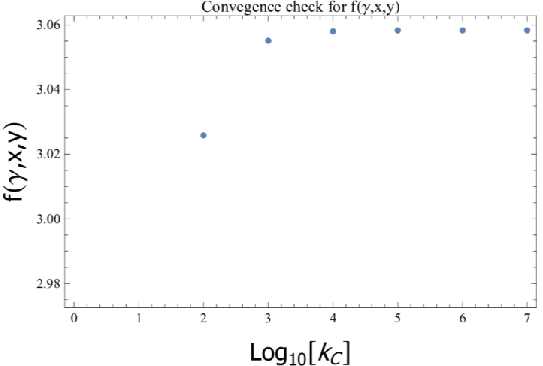
\includegraphics [width =0.7 \linewidth]{LHY_converge.pdf}
\end{center}
\caption[Convergence test of $f(\gamma ,x,y)$]{Convergence test of $f(\gamma ,x,y)$}  
\label{LHY_converge}
\end{figure}

% Minardi approximation
Now, we calculate $f(\gamma ,x,y)$ numerically for our Rb-Na Bose mixture system. First we do this integration and check its convergence. We plot $f(\gamma ,x,y)$ with increasing upper bound of integration $k_C$ to test its convergence, as shown in Fig. \ref{LHY_converge}. We can say that integration up to order of 6 has converged. Then, we calculate $f(\gamma ,x,y)$ with different $x$, i.e. with different B-field. Compare with Minardi's approximation
\cite{Minardi2019}, where they propose a analytical approximation which will be more convenient for deriving GPE with LHY correction. Here is the formula:
\begin{equation}
f(z,u=1,x)\simeq \left(1+z^{3/5}x\right)^{5/2}
\end{equation}
where
\begin{equation}
z=m_2/m_1, x=\frac{g_{22}n_2}{g_{11}n_1},u=\frac{g_{12}^2}{g_{11}g_{22}}
\end{equation}
Here, $u$ is set to be 1, because we only consider the case with near-zero MF energy, i.e. $g_{12}\approx\sqrt{g_{11}g_{22}}$ Now, we compare the numerical solution with the Minardi's approximation. Plot of List of f($\gamma $,x,y) for numerical one and Minardi's approximation. we can see that, there are mainly several percentage error by using this formula. And the maximum error is about 15$\%$. So, keep this error in mind about the LHY energy. (as show in Fig. \ref{LHY_Minardi})

% LHY_Minardi (done 2021-10-29 22:04:30)
\begin{figure}[htb]
\begin{center}
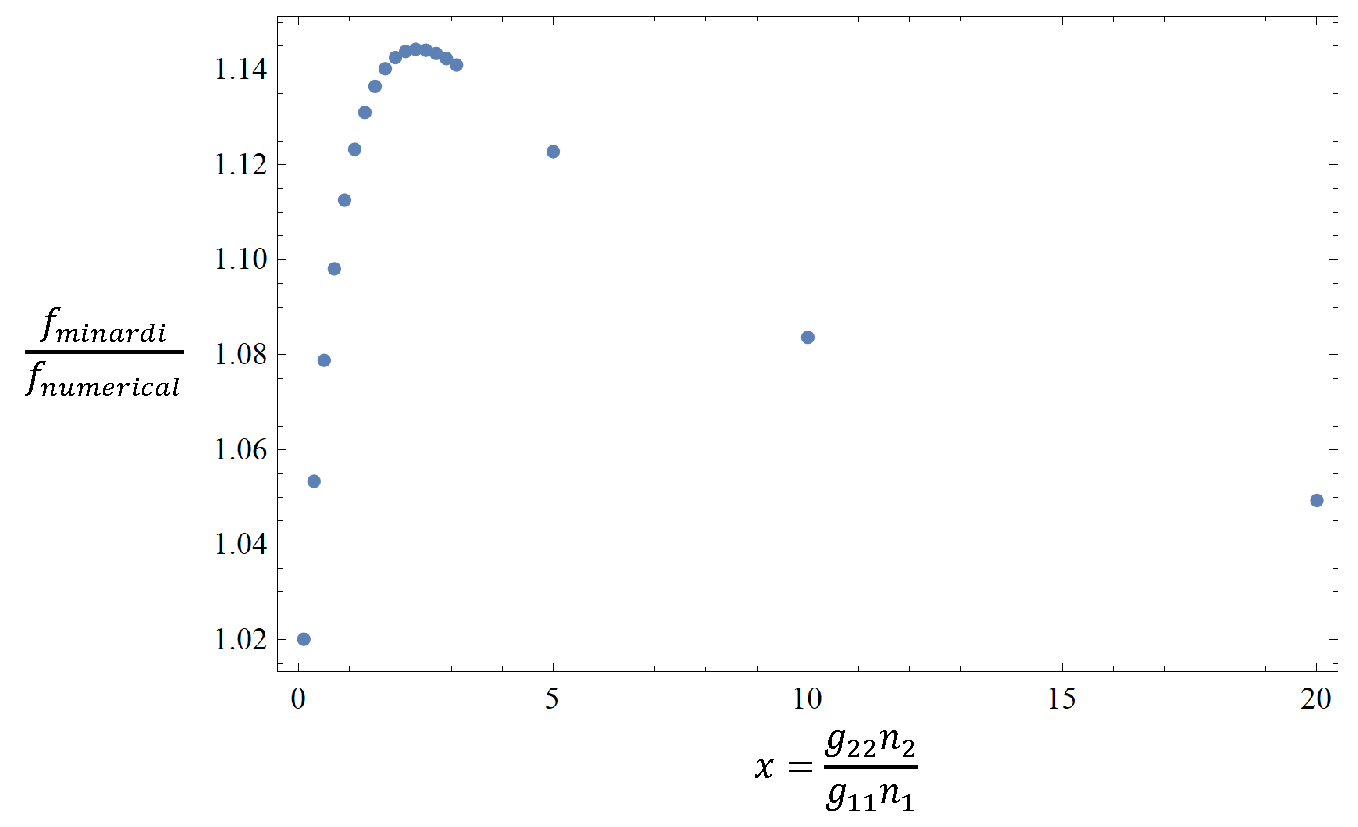
\includegraphics [width =0.85 \linewidth]{LHY_Minardi.pdf}
\end{center}
\caption[Compare the numerical solution and Minardi's approximation of $f(\gamma ,x,y)$]{Compare the numerical solution and Minardi's approximation of $f(\gamma ,x,y)$. The maxinum deviation is about 15\% when $g_{22}n_2/g_{11}n_1$ is around 2.}
\label{LHY_Minardi}
\end{figure}

% why we adopt this approximation (done 2021-10-29 22:04:52)
The subsequent GPE calculation requires a considerable amount of calculation. For example, for a 3D sample, if we split $2^7$ in each direction, then the calculation amount is to give an estimate. If the above infinite integral method is used to calculate the local of each grid LHY correction, then the amount of calculation will be huge. Therefore, if there is an analytical expression that can calculate the LHY correction, the amount of calculation will be significantly reduced. So Minardi approximation is a good starting point.

\subsection{Derivation of GPE for single species BEC}

% Derivation of single BEC GPE
First, we assume the many-body wave function is a product state
\begin{equation}
\Psi \left(\overset{\rightharpoonup }{r}_1,\overset{\rightharpoonup }{r}_2,\ldots  ,\overset{\rightharpoonup }{r}_N\right)=\sum _{i=1}^N \psi \left(\overset{\rightharpoonup}{r}_i\right)
\end{equation}
Then, we have
\begin{equation}
E\left(\psi ,\psi ^*\right)=N\int dr^3\left(\frac{\hbar ^2}{2m}\left| \nabla \psi (r)\right| ^2+V(r)\left| \psi (r)\right| ^2+\frac{1}{2}N g\left|\psi (r)\right| ^4\right)
\end{equation}
define the Variation
\begin{equation}
X\left(\psi ,\psi ^*\right)=E\left(\psi ,\psi ^*\right)-\mu  N\int dr^3\left| \psi (r)\right| ^2
\end{equation}
take the variation of $X\left(\psi ,\psi ^*\right)$, we have
\begin{equation}
\begin{split}
\delta  X\left(\psi ,\psi ^*\right)&=N\int dr^3\left[\frac{\hbar ^2}{2m}\left(\nabla \psi ^*(r)\nabla \delta \psi (r)+\nabla \psi (r)\nabla \delta \psi ^*(r)\right)\right.\\
&\left.\qquad\qquad+(V(r)-\mu )\left(\psi ^*(r)\delta  \psi (r)+\psi (r)\delta  \psi ^*(r) \right)\right.\\
&\left.\qquad\qquad+N g\left(\psi ^2(r)\delta  \psi ^*(r)+\psi ^{*2}(r)\delta\psi (r)\right)\right]\\
&=N\int dr^3\left[\frac{\hbar ^2}{2m}\left(\nabla \psi (r)\nabla \delta \psi ^*(r)\right)+(V(r)-\mu )\left(\psi (r)\delta  \psi ^*(r) \right)\right.\\
&\left.\qquad\qquad+N g\left(\psi^2(r)\psi ^*(r)\delta  \psi ^*(r)\right)\right]+c.c.
\end{split}
\end{equation}
for the first part, by using integrating by part method:
\begin{equation}
\begin{split}
\int dr^3\left(\nabla \psi (r)\nabla \delta \psi ^*(r)\right)&=\delta \psi ^*(r)\nabla \psi (r)|_0^{\infty }-\int dr^3\left(\nabla ^2\psi (r)\delta
\psi ^*(r)\right)\\
&=\int dr^3\left(-\nabla ^2\psi (r)\right)\delta \psi ^*(r)
\end{split}
\end{equation}
Then, take the variance to be zero, we have GPE
\begin{equation}
\begin{split}
-\frac{\hbar ^2}{2m}\left(\nabla ^2\psi (r)\right)+(V(r)-\mu )\psi (r)+N g\left(\psi ^2(r)\psi ^*(r)\right)=0\\
-\frac{\hbar ^2}{2m}\left(\nabla^2\psi^*(r)\right)+(V(r)-\mu)\psi ^*(r)+N g\left(\psi ^{*2}(r)\psi (r)\right)=0
\end{split}
\end{equation}

\subsection{Derivation of extended GPE for double species}
First, we assume the many-body wave function is a product state
\begin{equation}
\Psi \left(\overset{\rightharpoonup }{r}_1,\overset{\rightharpoonup }{r}_2,\ldots  ,\overset{\rightharpoonup }{r}_N\right)=\sum _{i=1}^N \psi \left(\overset{\rightharpoonup
}{r}_i\right)
\end{equation}
Then, we have
\begin{equation}
\begin{split}
E\left(\psi ,\psi ^*\right)=&N\int dr^3\left[\frac{\hbar ^2}{2m}\left(\nabla \psi ^*(r)\nabla \psi (r)\right)+V(r)\left(\psi ^*(r)\psi (r)\right)\right.\\
&\left.+\frac{1}{2}N g\left(\psi ^*(r)\psi (r)\right)^2+C \left(\psi ^*(r)\psi (r)\right)^{5/2}\right]
\end{split}
\end{equation}
define the Variation
\begin{equation}
X\left(\psi ,\psi ^*\right)=E\left(\psi ,\psi ^*\right)-\mu  N\int dr^3\left(\psi ^*(r)\psi (r)\right)
\end{equation}
take the variation of $X\left(\psi ,\psi ^*\right)$, we have
\begin{equation}
\begin{split}
\delta  X\left(\psi ,\psi ^*\right)&=N\int dr^3\left[\frac{\hbar ^2}{2m}\left(\nabla ^2\psi (r)\delta \psi ^*(r)\right)+(V(r)-\mu )\left(\psi (r)\delta\psi ^*(r) \right)\right.\\
&\left.+N g\left(\psi ^2(r)\psi ^*(r)\delta \psi ^*(r)\right)+\frac{5C}{2}(\psi (r))^{5/2}\left(\psi ^*(r)\right)^{3/2}\delta \psi ^*(r)\right]+c.c.
\end{split}
\end{equation}
where C is constants which already expressed the Last Part.
thus, we have eGPE
\begin{equation}
-\frac{\hbar ^2}{2m}\nabla ^2\psi (r)+(V(r)-\mu )\psi (r)+N g\left|\psi (r)\right|^2\psi(r)+\frac{5C}{2}\left|\psi (r)\right|^3\psi (r)=0
\end{equation}

% double species BEC
First, we assume the many-body wave function is a product state
\begin{equation}
\Psi \left(\overset{\rightharpoonup }{r}_1,\overset{\rightharpoonup }{r}_2,\ldots  ,\overset{\rightharpoonup }{r}_N\right)=\sum _{i=1}^N \psi _1\left(\overset{\rightharpoonup
}{r}_i\right)\sum _{i=1}^N \psi _2\left(\overset{\rightharpoonup }{r}_i\right)
\end{equation}
Then, we have
\begin{equation}
E\left(\psi _1,\psi _1{}^*,\psi _2,\psi _2{}^*\right)=\int dr^3\left(
\begin{array}{cc}
 \psi _1^* & \psi _2^* \\
\end{array}
\right).\left(
\begin{array}{cc}
 \mathcal{H}_{11} & \mathcal{H}_{12} \\
 \mathcal{H}_{21} & \mathcal{H}_{22} \\
\end{array}
\right).\left(
\begin{array}{c}
 \psi _1 \\
 \psi _2 \\
\end{array}
\right)+E_{\text{LHY}}
\end{equation}

where $\mathcal{H}_{ij}$ represent the Hamiltonian density of fields
\begin{equation}
\begin{split}
\mathcal{H}_{11}&=N_1\left(\frac{\hbar ^2}{2m_1}(\nabla )^2+V_1(r)+\frac{1}{2}N_1g_{11}\left(\psi _1{}^*(r)\psi _1(r)\right)\right)\\
\mathcal{H}_{22}&=N_2\left(\frac{\hbar ^2}{2m_2}(\nabla )^2+V_2(r)+\frac{1}{2}N_2g_{22}\left(\psi _2{}^*(r)\psi _2(r)\right){}^2\right)\\
\mathcal{H}_{12}&=\mathcal{H}_{21}^{\dagger }=N_1N_2g_{12}\left(\psi _1{}^*(r)\psi _1(r)\right)\left(\psi _2{}^*(r)\psi _2(r)\right)
\end{split}
\end{equation}
and LHY term has been expressed in the last part.
define the Variation
\begin{equation}
X\left(\psi ,\psi ^*\right)=E\left(\psi ,\psi ^*\right)-\mu _1 N_1\int dr^3\left(\psi _1{}^*(r)\psi _1(r)\right)-\mu _2 N_2\int dr^3\left(\psi
_2{}^*(r)\psi _2(r)\right)
\end{equation}

Finally, we have eGPE for 
\begin{equation}
\begin{split}
i \hbar \frac{\partial\psi_1}{\partial t}=\left(-\frac{\hbar^2\nabla^2}{2m_1}+V_1+g_{11}n_1+g_{12}n_2+\frac{\delta  \mathcal{E}_{\text{LHY}}}{\delta n_1}\right)\psi _1\\
i \hbar \frac{\partial \psi _2}{\partial t}=\left(-\frac{\hbar ^2\nabla ^2}{2m_2}+V_2+g_{22}n_2+g_{12}n_1+\frac{\delta  \mathcal{E}_{\text{LHY}}}{\delta n_2}\right)\psi _2
\end{split}
\end{equation}

\subsection{eGPE for GPELAB with Minardi approximation}

\begin{equation}
\begin{split}
i \hbar \frac{\partial\psi_1}{\partial t}=\left(-\frac{\hbar^2\nabla^2}{2m_1}+V_1+g_{11}n_1+g_{12}n_2+\frac{\delta  \mathcal{E}_{\text{LHY}}}{\delta n_1}\right)\psi _1\\
i \hbar \frac{\partial \psi _2}{\partial t}=\left(-\frac{\hbar ^2\nabla ^2}{2m_2}+V_2+g_{22}n_2+g_{12}n_1+\frac{\delta  \mathcal{E}_{\text{LHY}}}{\delta n_2}\right)\psi _2
\end{split}
\end{equation}
where$n_i=N_i\psi _i^*\psi _i=N_i|\psi _i|^2$ and 
\begin{equation}
\frac{\delta  \mathcal{E}_{\text{LHY}}}{\delta  n_1}=\frac{8}{15\pi^2}\frac{m_1^{3/2}\left(g_{11}\right){}^{5/2}n_1^{1/2}}{\hbar^3}\left(\frac{5}{2}n_1f(\gamma,x,y)-\frac{g_{22}n_2}{g_{11}}\frac{\partial f(\gamma ,x,y)}{\partial y}\right)
\end{equation}
\begin{equation}
\frac{\delta  \mathcal{E}_{\text{LHY}}}{\delta  n_2}=\frac{8}{15\pi^2}\frac{m_1^{3/2}\left(g_{11}\right){}^{3/2}g_{22}n_1^{3/2}}{\hbar ^3}\frac{\partial
f(\gamma ,x,y)}{\partial y}
\end{equation}
if we using the approximation formula, we have
\begin{equation}
\mathcal{E}_{\text{LHY}}=\frac{8}{15\pi ^2}\frac{m_1^{3/2}\left(g_{11}n_1\right){}^{5/2}}{\hbar ^3}\left(1+\gamma ^{3/5}y\right)^{5/2}
\end{equation}
Then, 
\begin{equation}
\begin{split}
\frac{\delta  \mathcal{E}_{\text{LHY}}}{\delta  n_1}&=\frac{8}{15\pi^2}\frac{m_1^{3/2}\left(g_{11}\right){}^{5/2}n_1^{1/2}}{\hbar^3}\left(\frac{5}{2}n_1\left(1+\gamma^{3/5}y\right){}^{5/2}-\frac{5}{2}\frac{g_{22}n_2}{g_{11}}\left(1+\gamma ^{3/5}y\right)^{3/2}\gamma ^{3/5}\right)\\
&=\frac{4}{3\pi^2}\frac{m_1^{3/2}\left(g_{11}\right){}^{5/2}n_1^{3/2}}{\hbar^3}\left(1+\gamma^{3/5}y\right)^{3/2}
\end{split}
\end{equation}
\begin{equation}
\begin{split}
\frac{\delta  \mathcal{E}_{\text{LHY}}}{\delta n_2}&=\frac{8}{15\pi^2}\frac{m_1^{3/2}\left(g_{11}\right){}^{3/2}g_{22}n_1^{3/2}}{\hbar^3}\frac{5}{2}\left(1+\gamma^{3/5}y\right)^{3/2}\gamma ^{3/5}\\
&=\frac{4}{3\pi^2}\frac{\gamma^{3/5}m_1^{3/2}\left(g_{11}\right){}^{3/2}g_{22}n_1^{3/2}}{\hbar^3}\left(1+\gamma ^{3/5}y\right)^{3/2}
\end{split}
\end{equation}
Finally, we have extended GPE as
\begin{equation}
\begin{split}
i \hbar \frac{\partial \psi _1}{\partial t}=\left(-\frac{\hbar ^2\nabla ^2}{2m_1}+V_1+g_{11}n_1+g_{12}n_2+\frac{4}{3\pi ^2}\frac{g_{11}m_1^{3/5}}{\hbar
^3}\left(g_{11}n_1m_1^{3/5}+g_{22}n_2m_2^{3/5}\right){}^{3/2}\right)\psi _1\\
i \hbar \frac{\partial \psi _2}{\partial t}=\left(-\frac{\hbar ^2\nabla ^2}{2m_2}+V_2+g_{22}n_2+g_{12}n_1+\frac{4}{3\pi ^2}\frac{g_{22}m_2^{3/5}}{\hbar
^3}\left(g_{11}n_1m_1^{3/5}+g_{22}n_2m_2^{3/5}\right){}^{3/2}\right)\psi _2
\end{split}
\end{equation}
Now, we need do Dimension-Reduction, 
\begin{equation}
\begin{split}
i \frac{\partial \Psi _1}{\partial T}&=\left[-\frac{m\pmb{\nabla }^2}{2m_1}+\frac{V_1}{\hbar  \omega }+4\pi  \frac{m}{m_1}\frac{ N_1a_{11}}{a}\Psi_1^*\Psi _1+2\pi \frac{ m }{m_{12}}\frac{N_2a_{12}}{a}\Psi _2^*\Psi _2\right.\\
&\left.+\frac{128\pi ^{1/2} }{3} \frac{a_{11}}{a}\left(\frac{m}{m_1}\right){}^{2/5}\left(\frac{N_1a_{11}}{a}\left(\frac{m}{m_1}\right){}^{2/5}\Psi _1^*\Psi _1\right.\right.\\
&\left.\left.+ \frac{N_2a_{22}}{a}\left(\frac{m}{m_2}\right){}^{2/5}\Psi _2^*\Psi _2\right){}^{3/2}\right]\Psi_1\\
i \frac{\partial \Psi _2}{\partial T}&=\left[-\frac{m\pmb{\nabla }^2}{2m_2}+\frac{V_2}{\hbar  \omega }+4\pi  \frac{m}{m_2}\frac{\text{  }N_2a_{22}}{a}\Psi_2^*\Psi _2+2\pi \frac{ m }{m_{12}}\frac{N_1a_{12}}{a}\Psi _1^*\Psi _1\right.\\
&\left.+\frac{128\pi ^{1/2} }{3}\frac{a_{22}}{a}\left(\frac{m}{m_2}\right){}^{2/5}\left(\frac{N_1a_{11}}{a}\left(\frac{m}{m_1}\right){}^{2/5}\Psi _1^*\Psi _1\right.\right.\\
&\left.\left.+ \frac{N_2a_{22}}{a}\left(\frac{m}{m_2}\right){}^{2/5}\Psi _2^*\Psi _2\right){}^{3/2}\right]\Psi_2
\end{split}
\end{equation}
where we set $V_1$ and $V_2$ as harmonic trap, and it gives the characteristic length and time. Actually, this characteristic length and time can be arbitrary.
\begin{equation}
\begin{split}
g_{11}=\frac{4\pi  \hbar ^2a_{11}}{m_1}, g_{22}=\frac{4\pi  \hbar ^2a_{22}}{m_2}, g_{12}=\frac{2\pi  \hbar ^2a_{12}}{m_{12}}, m_{12}=\frac{m_1m_2}{m_1+m_2}\\
T=\omega  t, \overset{\rightharpoonup }{R}=\left.\overset{\rightharpoonup }{r}\right/a, \Psi =\psi  a^{3/2}, a=\sqrt{\frac{\hbar }{m \omega }}
\end{split}
\end{equation}
By the way, we can calculate the Nonlinear-Energy function. (Just for fun, not for GPELAB)
Recall LHY energy term
\begin{equation}
\begin{split}
\mathcal{E}_{\text{LHY}}=\frac{8}{15\pi ^2}\frac{m_1^{3/2}\left(g_{11}n_1\right){}^{5/2}}{\hbar ^3}\left(1+\left(\frac{m_2}{m_1}\right){}^{3/5}\frac{g_{22}n_2}{g_{11}n_1}\right){}^{5/2}\\
=\frac{256\sqrt{\pi }\hbar ^2}{15}\left(m_1^{-2/5}a_{11}n_1+m_2^{-2/5}a_{22}n_2\right){}^{5/2}
\end{split}
\end{equation}
Do Dimension-Reduction, we have
\begin{equation}
\frac{\mathcal{E}_{\text{LHY}}}{\hbar\omega\left/a^3\right.}=\frac{256\pi^{1/2}}{15}\left(\frac{N_1a_{11}}{a}\left(\frac{m}{m_1}\right){}^{2/5}\Psi_1^*\Psi_1+\frac{N_2a_{22}}{a}\left(\frac{m}{m_2}\right){}^{2/5}\Psi _2^*\Psi _2\right){}^{5/2}
\end{equation}

\section{Na-Rb Hetero-nuclear quantum droplet}
\label{sec:droplet_experiment}

This section\footnote{This section is mainly from our paper \cite{guo2021leehuangyang}.} demonstrates our experiment study on the quantum droplet made of Na-Rb BEC mixture. Our experiment starts from an optically trapped double BEC of $^{23}$Na and $^{87}$Rb (denoted as species 1 and 2 hereafter, respectively) both prepared in their lowest-energy hyperfine Zeeman level $\ket{F = 1, m_F = 1}$~\cite{wang2015double}. To reveal the LHY effects, we focus on the near-zero MF region with $\delta g = g_{12} + \sqrt{g_{11} g_{22}} \approx 0$. Here $g_{ij} = 2\pi\hbar^2 a_{ij}/M_{ij}$ are the two-body interaction constants, with $a_{ij}$ the scattering lengths and $M_{ij}$ the reduced masses. To reach this regime, we use the Na-Rb Feshbach resonance at $B_0 = 347.648$~G to tune the Na-Rb scattering length. The scattering length is represented as $a_{12} = a_\text{bg}\big(1-\Delta/(B-B_0)\big)$ [upper panel of Fig.~\ref{fig1}(a)], with background scattering length $a_\text{bg} = 76.33a_0$ and resonance width $\Delta = 4.255$~G~\cite{wang2013observation}. Near $B_0$ the intraspecies scattering lengths $a_{11} = 60.05a_0$~\cite{Knoop2011} and $a_{22} = 100.13a_0$~\cite{Kempen2002} remain almost constant. 

%% add figure1 here
\begin{figure}[hbt]
\begin{center}
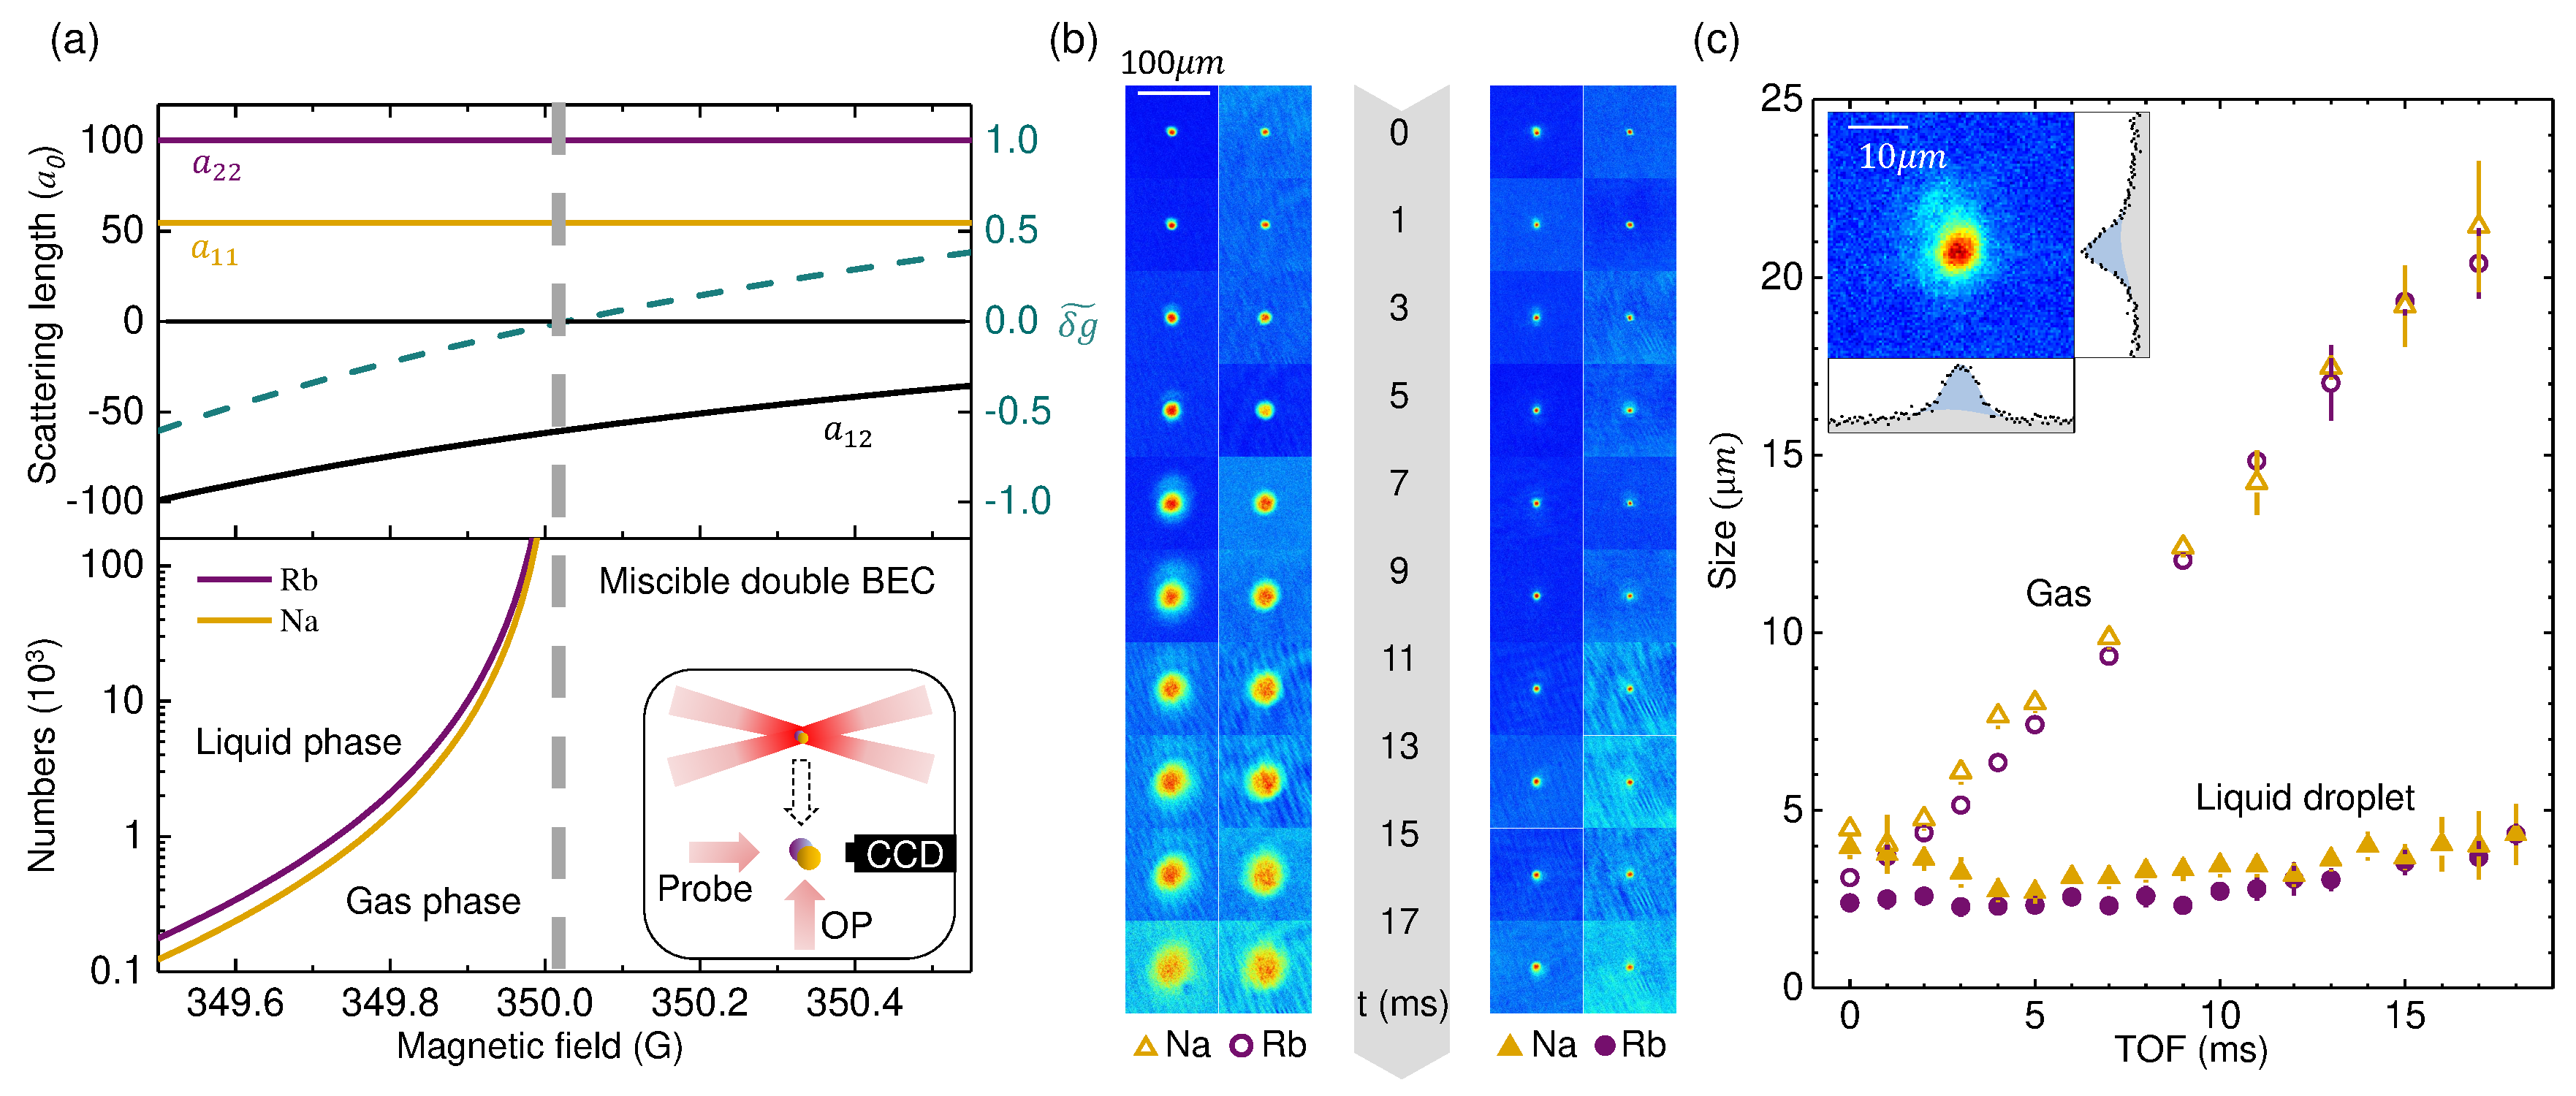
\includegraphics [width = \linewidth]{fig1.pdf}
\end{center}
\caption[Creation and detection of Na-Rb mixtures for investigating LHY effects]{Creation and detection of Na-Rb mixtures for investigating LHY effects. (a) In the upper panel, the purple, yellow, and black solid lines are scattering lengths between Na-Na($a_{11}$), Rb-Rb($a_{22}$) and Na-Rb($a_{12}$), respectively. The dashed green curve is $\widetilde{\delta g}$. The dashed vertical line indicates the magnetic field for $\widetilde{\delta g} = 0$. In the lower panel, the phase diagrams at different atomic numbers and magnetic fields are shown. Inset: schematic detection method of the droplet in free space. (b) Images of the mixture during the TOF expansion in the gas phase at 350.451 G (left) and the droplet phase at 349.849 G (right). (c) Cloud sizes obtained from (b) reveal the very different behaviors of the two phases. Data points for $^{87}$Rb are shown in purple, while those for $^{23}$Na are in yellow. Inset: in the droplet phase, 
bimodal distributions are observed for the cloud with excess atoms. A double Gaussian fitting is used to extract the droplet size in this case.
}
\label{fig1}
\end{figure}
%% add figure1 here

For convenience, we define a dimensionless parameter $\widetilde{\delta g} \equiv \delta g/\overline{g}$ to characterize the total $E_{\rm MF}$, with $\overline{g} = (g_{11}+g_{22})/2$. For the current system, the critical magnetic field for $\widetilde{\delta g} = 0$ (and also $\delta g= 0$) is $B_c = 349.978$~G, which corresponds to a critical interspecies scattering length $a^c_{12} = -63.1 a_0$. As shown in Fig.~\ref{fig1}(a) (lower panel), for each value of $\widetilde{\delta g} < 0$, the double BEC will undergo a transition from gas phase to droplet phase as the atom numbers are increased. With our atom numbers around $10^4$ for both species, the theory predicts an observation window for the droplet phase for $\widetilde{\delta g}$ from $-0.061$ to $-0.189$ (349.910 G to 349.780 G). For $\widetilde{\delta g}$ from 0 to $-0.061$, droplet formation is still possible but atom numbers much larger than currently available are needed.

\subsection{Experiment method and time sequence}

%imaging method
In the first experiment, we study the Na-Rb quantum droplet in free space by releasing the sample from the optical trap. We probe the system during the time of flight (TOF), as depicted in the inset of Fig.~\ref{fig1}(a). To probe the atoms in situ at each TOF, we implement a two-species high-field detection protocol which consists of a partial optical pumping process followed by standard absorption imaging on the cycling transitions~\cite{jia2020}. This partial imaging method is necessary as the droplets have very high optical depth and are difficult to detect directly~\cite{ramanathan2012partial,semeghini2018self}. Both the partial optical pumping and the absorption imaging are calibrated using standard methods~\cite{reinaudi2007strong,hueck2017calibrating}. The measured resolutions ($1/\sqrt{e}$ half Gaussian widths) of our imaging system are $0.6~\mu$m and $0.8~\mu$m for $^{23}$Na at 589 nm and $^{87}$Rb at 780 nm, respectively, which are just enough to resolve the droplet. To maintain the imaging resolutions, we mount the objective and the probe light optics on high-precision vertical translational stages to keep the optical axis of the imaging system always aligned with the droplet.

%experiment method and time sequence
Figure \ref{droplet_time_sequence} shows the time sequence we produce quantum droplet. While shutting down the optical trap provides a direct way of probing the droplet in free space, the non-adiabatic nature of the process can cause problems. Due to the confinement, the in-trap sample is smaller in size than the free-space droplet in its ground state, while the total energy of the system is much larger. In the worst scenario, the energy of the initial state upon release from the trap is larger then the energy barrier of the expansion and a stable droplet can never be formed. To mitigate this problem, the crossed optical dipole trap is configured in a nearly spherical shape with measured trap oscillation frequencies of 78 Hz (86 Hz) for $^{87}$Rb ($^{23}$Na). This is in accordance with the understanding that a quantum droplet with isotropic short-range interactions should be spherical in free space. In addition, a carefully designed magnetic field control sequence is used to improve the mode matching. These steps allow us to observe droplet formation reliably for $\widetilde{\delta g}$ from $-0.094$ to $-0.189$. However, for $\widetilde{\delta g}$ from $-0.061$ to $-0.094$, due to the smaller binding energy, droplets can be observed only by a more sophisticated mode-matching method, aided by fast magnetic field quenching at the instant of releasing the samples from the trap. For this method to work, the starting magnetic field must be selected carefully so that the size of the in-trap sample matches that of the free-space droplet at the end of the magnetic field quenching.

% time sequence
\begin{figure}[hbt]
\begin{center}
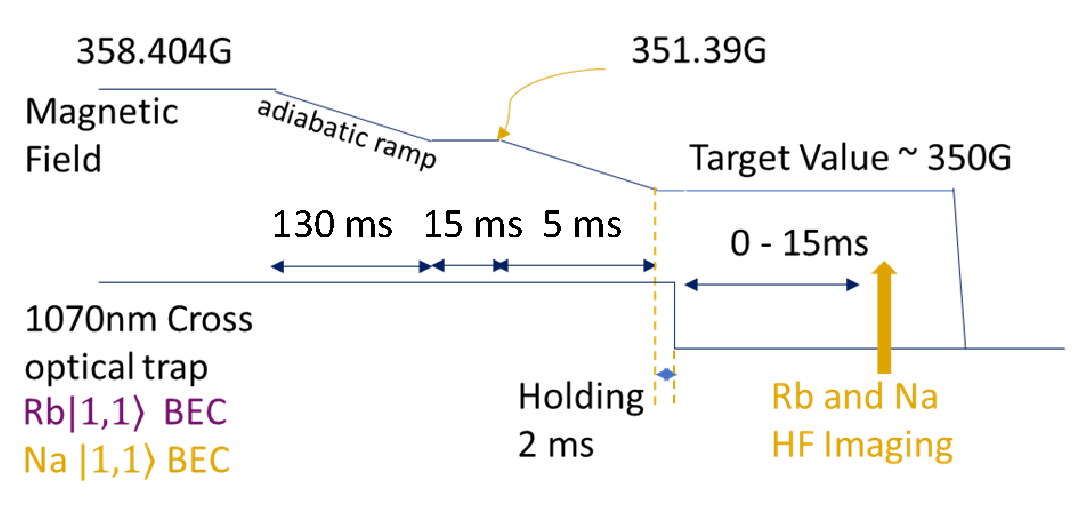
\includegraphics[width = 0.8\linewidth]{figures/droplet_time_sequence.pdf}
\end{center}
\caption[Time sequence for producing quantum droplet]{Time sequence for producing quantum droplet.}
\label{droplet_time_sequence}
\end{figure}

\subsection{observing non-expansion signal}

Figure~\ref{fig1}(b) shows a side-by-side comparison of the $^{23}$Na and $^{87}$Rb clouds in the gas phase and the droplet phase following the TOF. The signature self-bound behavior of the droplet can be observed clearly by comparing its dramatically different TOF expansion with that in the gas phase. For $\widetilde{\delta g}=-0.119$ (349.849 G), where the droplet phase is expected, the sizes of both clouds stay nearly the same during the TOF. For $\widetilde{\delta g}=+0.344$ (350.451 G), by contrast, the system remains in the gas phase, and the sizes increase steadily with TOF.

% fitting by Gaussian and double-Gaussian
To extract quantitative information, we fit the images with 2D Gaussian functions. In the droplet, the size should be the same for the two species; their densities and thus numbers should follow the ratio $N_{2}/N_{1} = \sqrt{g_{11}/g_{22}}=1.51$~\cite{petrov2015}. When this ratio is not maintained, the droplet part shows up as a dense central peak, and the excess atoms of one species appear as a much larger-sized and expanding gaseous background surrounding the droplet [inset of Fig.~\ref{fig1}(c)]. For this kind of ``bimodal'' distribution, the droplet parameters are extracted with a double 2D Gaussian fitting. Fig.~\ref{fig1}(c) shows the starkly different expansion behaviors in the droplet and the gas phases obtained from the images in Fig.~\ref{fig1}(b).

%% add figure2 here
\begin{figure}[htb]
\begin{center}
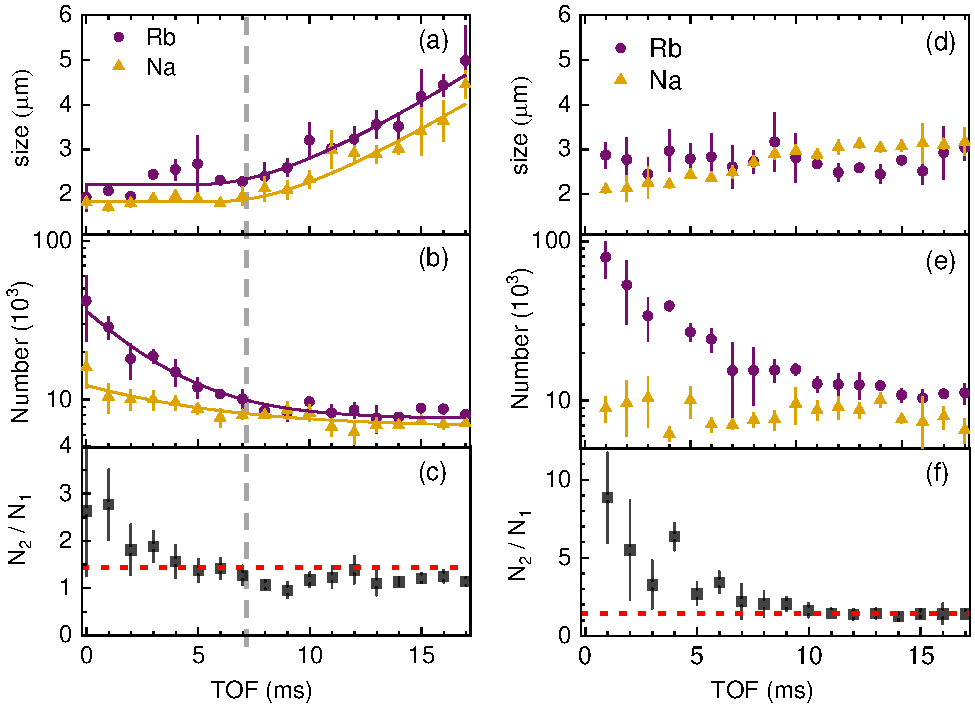
\includegraphics [width =0.95 \linewidth]{fig2.pdf}
\end{center}
\caption[Evolution of the Na-Rb droplet in free space]{Evolution of the Na-Rb droplet in free space. (a), (b), and (c) show the size, atom numbers, and the $^{87}$Rb to $^{23}$Na number ratio at $\widetilde{\delta g} = -0.116$ (349.852 G) following the TOF. The droplet is created by directly releasing the sample from the trap. The vertical bar marks the approximate time of the liquid-to-gas phase transition. (d), (e), and (f) show the evolution for the droplet created with the additional magnetic field quenching for $\widetilde{\delta g} = -0.089$ (349.880 G). The red dashed lines in (c) and (f) mark the theoretical number ratio $N_2/N_1=1.51$.}  
\label{fig2}
\end{figure}

%Explanation of Fig#2
%droplet formation
For the droplets formed by direct trap release from $\widetilde{\delta g} = -0.094$ to $-0.189$, we observe two distinctively different dynamics in the evolution of the $^{23}$Na and $^{87}$Rb samples during the TOF. As an example, Fig.~\ref{fig2}(a), (b) and (c) show the sizes, atom numbers, and number ratio of the droplet sample for $\widetilde{\delta g}=-0.116$ (349.852~G).
During the first 10 ms, the $^{23}$Na and $^{87}$Rb sizes increase very little, while atom losses are observed for both species.
Bimodal distributions are observed from 0 ms to 5 ms as the initial number ratio is far from 1.51. After 5 ms expansion, the gaseous atoms surrounding the droplet are already too dilute to be detected. 

%droplet to the gas phase transition
After about 10 ms, the sample sizes start to increase while the atom numbers stay nearly constant.
This is consistent with a phase transition from droplet to gas when the atom numbers are reduced to below the critical values [see Fig.~\ref{fig1}(a)]. We fit the size evolution empirically with $\sigma(t>t_0)=\sqrt{\sigma_0^2+v^2(t-t_0)^2}$ and $\sigma(t<t_0)=\sigma_0$, and obtain a lifetime in the droplet phase of about $t_0 = 7$ ms. Here $v$ is the expansion velocity of the gas-phase sample. Similarly, as illustrated in Fig.~\ref{fig2}(b), the critical atom numbers for the phase transition can be obtained by fitting the $^{23}$Na and $^{87}$Rb number evolution data with an 
exponential decay function with the critical number as the offset.

For several values of $\widetilde{\delta g}$ between $-0.061$ and $-0.094$, we have created longer-lived droplets by the magnetic field quenching method. As shown in Fig.~\ref{fig2}(d), (e) and (f), during the accessible TOF, the droplet size stays nearly the same although number losses are still observed. After 10 ms, the number ratio becomes close to 1.51 and the number loss slows down significantly. As the lifetime is longer than the usable TOF of 18 ms, we have not been able to measure the real lifetime and the critical numbers in this range of $\widetilde{\delta g}$. More detailed investigations, e.g., by levitating the droplet, are warranted in the near future.

\subsection{Characterization of liquid-gas phase transition}

Figure~\ref{fig3} shows the critical $^{23}$Na and $^{87}$Rb atom numbers for $\widetilde{\delta g}$ from $-0.146$ to $-0.247$. Although the range of $\widetilde{\delta g}$ is small, a four-fold change in the measured critical numbers is observed. The critical numbers calculated using coupled eGPEs with the LHY term included (dashed curves) show large discrepancies with the measurements. The agreement is greatly improved by also including the small post-compensation residual magnetic field gradient in the eGPEs (solid curves); the additional term nearly doubles  the critical numbers. This can be understood from the different magnetic dipole moments and masses of $^{23}$Na and $^{87}$Rb, which cause their centers of mass to separate in a magnetic field gradient. This decreases the density overlap and lowers the attractive interspecies mean-field energy while leaving the intraspecies energy nearly intact. Effectively, this increases the critical numbers compared to the ideal case of zero gradient.

%% add figure3 here
\begin{figure}[htb]
\begin{center}
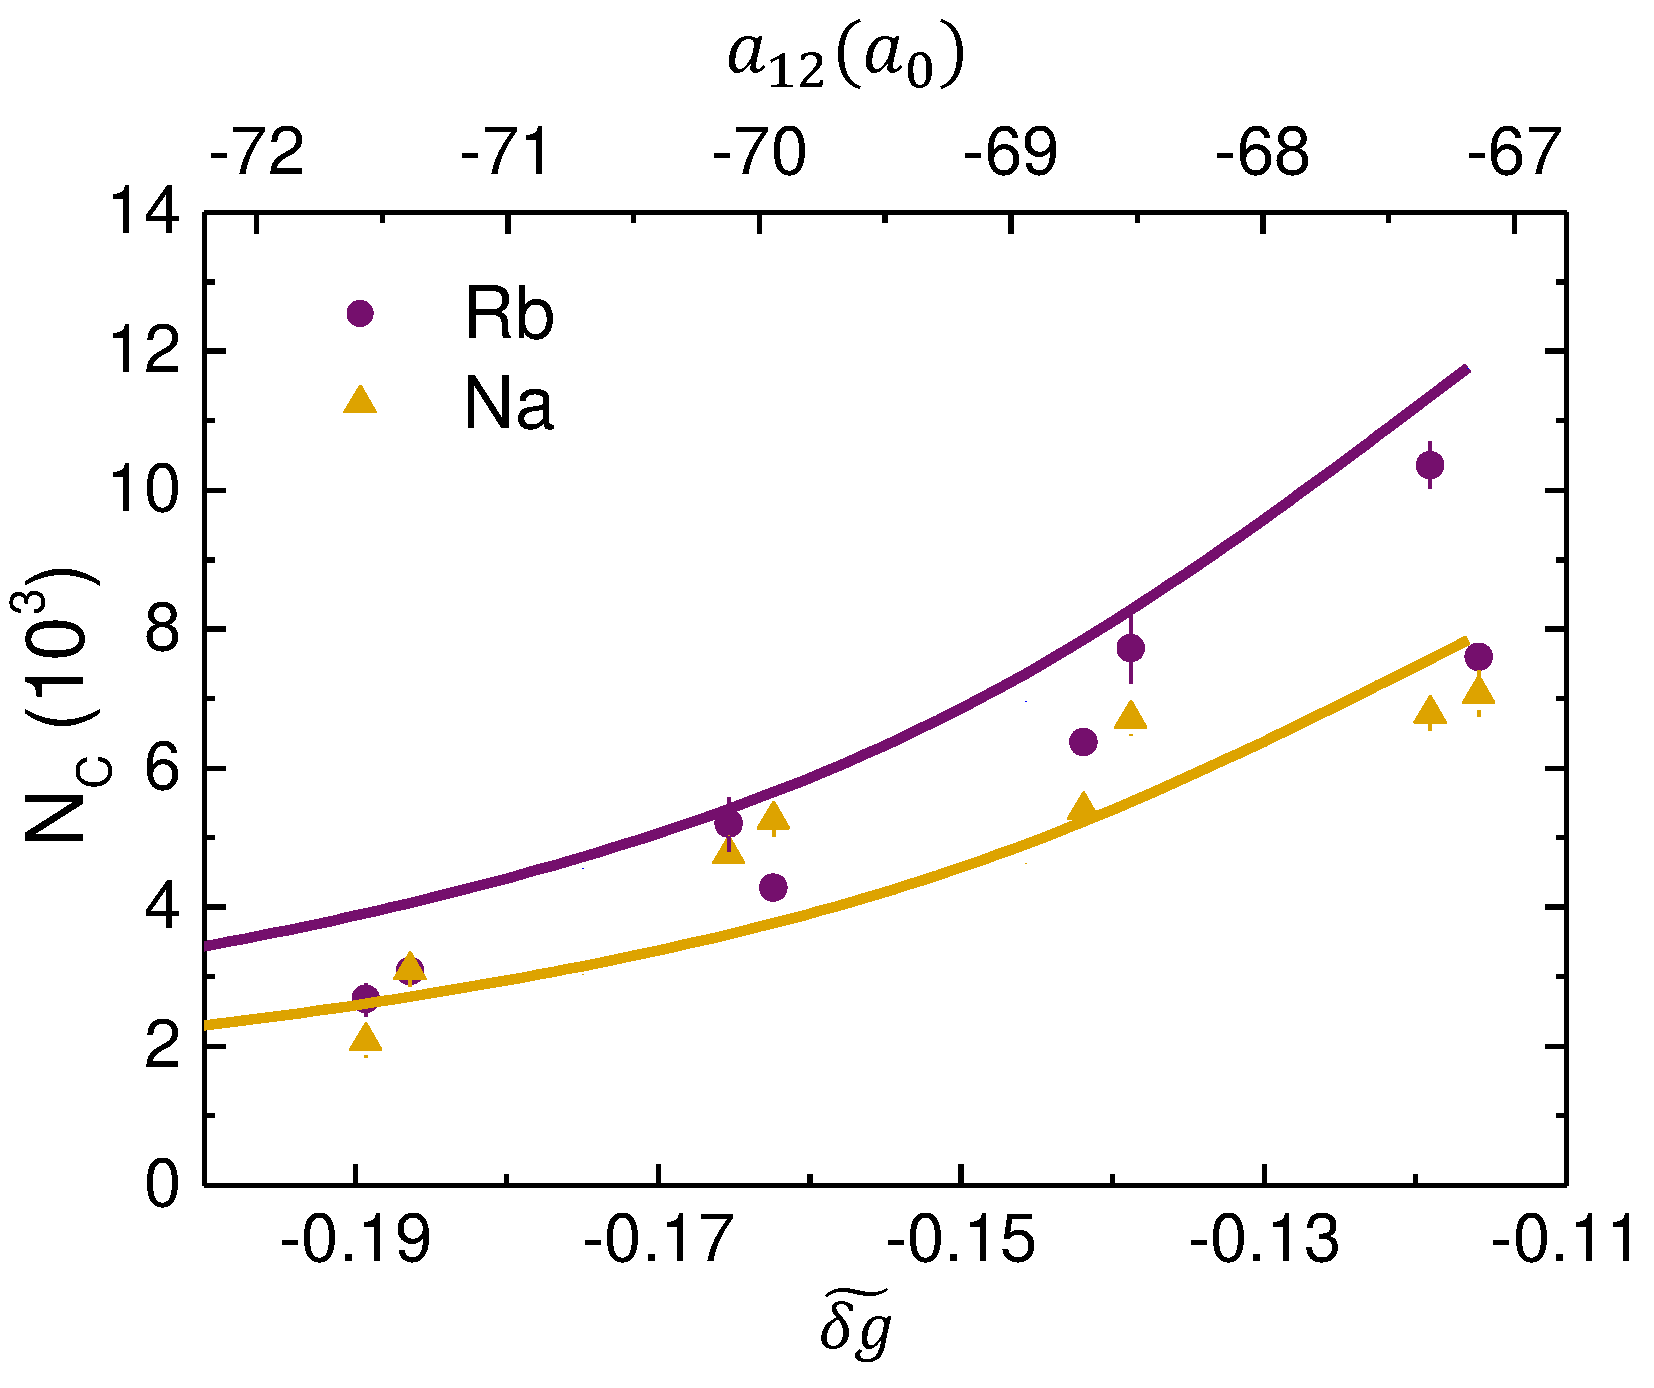
\includegraphics [width =0.85 \linewidth]{fig3.pdf}
\end{center}
\caption[Critical atom numbers for the liquid-to-gas phase transition as a function of $\widetilde{\delta g}$]{Critical atom numbers for the liquid-to-gas phase transition as a function of $\widetilde{\delta g}$. The solid lines are calculated from coupled eGPEs with the residual magnetic field gradient included.}
\label{fig3}
\end{figure}
%% add figure3 here

% about loss
A major cause of the atom losses is three-body recombination as a result of the high number densities in the droplet~\cite{cabrera2018quantum,semeghini2018self,DErrico2019}. For droplets with $\widetilde{\delta g}$ from $-0.094$ to $-0.189$, another possible loss mechanism is self-evaporation due to the imperfect matching between in-trap and free-space modes~\cite{Ferioli2020}. The short lifetimes in this region are the combined result of these loss mechanisms. In contrast, the droplet at $\widetilde{\delta g} = -0.089$ [see Fig.~\ref{fig2}(d), (e), and (f)] has relatively lower number densities and is formed with nearly optimal mode matching, and is thus longer lived. Nevertheless, for both cases, the stabilized number ratios after 10 ms TOF are very close to 1.51 despite the different creation procedures and the large initial number mismatches [Fig.~\ref{fig2}(c) and (f)].

\section{Lee-Huang-Yang gas}
\label{sec:LHY_gas}

We now turn to the gas-phase double BEC and release the sample directly from the trap (without the additional magnetic field quenching) for $\widetilde{\delta g}$ from +0.344 to $-0.094$. To characterize the LHY effect, we measure the release energy $E_{\rm rel}=E_{\rm kin}+E_{\rm int}$ from the TOF expansion~\cite{Holland1997,Mewes1996}. Here $E_\text{\rm kin}$ is the quantum pressure and $E_{\rm int}=E_{\rm MF}+E_{\rm LHY}$ is the total interaction energy. When $E_{\rm MF}$ is tuned to zero, $E_{\rm LHY}$ becomes the only interaction term in $E_{\rm rel}$. For negative $E_{\rm MF}$, the fact that the sample expands rather than collapses is also a direct manifestation of the LHY effect.

When we using TOF measurement on condensate from a harmonic trap, we lose the trap energy suddenly and the kinetic energy (quantum pressure) and the interaction energy converts to kinetic energy of motion after long-time evolution. So, we have the release energy
\begin{equation}
E_{\text{release}}=E_{\text{kin}}+E_{\text{MF}}=N \hbar  \omega _0\left(\frac{3}{4}\frac{1}{w^2}+\frac{1}{\sqrt{2\pi }}\frac{a_SN}{a_{\text{ho}}}\frac{1}{w^3}\right)
\end{equation}
put the numerical solution of $w$ into the release energy, we have for $g=0 \text{case}$, we have $E_{\text{release}}=\frac{3}{4}\hbar \omega _0$ With increasing $\chi$, we have larger size (larger $w$), and finally, when reach $\chi >>1$ limit, we turn to the Thomas-Fermi limit.

\subsection{Expansion of gas phase sample and Release energy}
%introduce the LHY gas, explain the difference between liquid droplet and LHY gas
In the previous sections, we describe a liquid phase droplet sample made of $^{23}\rm Na$--$^{87}\rm Rb$ BEC mixture. Now we turn to study the gas phase (LHY gas) of this mixture, in which the Lee-Huang-Yang effects still play an important role. The mainly difference between a droplet and a LHY gas sample is whether the kinetic energy dominates the Hamiltonian. For droplet sample, the competition mainly comes from the attractive mean-field term and the repulsive LHY term. When the atomic number drops down, and both mean-field and LHY energy goes down, finally the kinetic energy gets not negligible. After the balance point of density disappeared, as we describe about the liquid-gas phase transition, the sample turns to a gas-phase sample.

by directly releasing the sample from the trap for $\widetilde{\delta g}$ from +0.322 to -0.146.
To characterize the LHY effect in this situation, we measure the release energy $E_{\rm rel}=E_{\rm kin}+E_{\rm int}$ from the TOF expansion~\cite{Holland1997,Mewes1996}. Here $E_\text{\rm kin}$ is the quantum pressure and $E_{\rm int}=E_{\rm MF}+E_{\rm LHY}$ is the total interaction energy. When $E_{\rm MF}$ is tuned to zero, $E_{\rm LHY}$ becomes the only interaction term in $E_{\rm rel}$. For negative $E_{\rm MF}$, the expansion of the sample, instead of collapsing, is also a direct manifestation of the LHY effect. 

We prepared the trapped double BEC and measured $E_{\rm rel}$ for both species from their TOF expansion velocities~\cite{Holland1997} for several different $\widetilde{\delta g}$. The resulting total $E_{\rm rel}$ is shown as open squares in Fig.~\ref{fig4}. In general, $E_{\rm rel}$ depends on $\widetilde{\delta g}$, $N_1$ and $N_2$, and the density overlap between the two species. However, within the range of $\widetilde{\delta g}$, the densities of the double BEC are still rather high even in the gas phase, and significant three-body losses are still observed during the TOF. Thus, it is difficult to maintain constant $N_1$ and $N_2$ during the TOF for different $\widetilde{\delta g}$, even though great efforts have been taken to keep the initial atom numbers in the trap fixed. However, since $E_{\rm rel}$ is a measure of the energy per atom, it is not affected severely by the loss. 

\begin{figure}[hbt]
\begin{center}
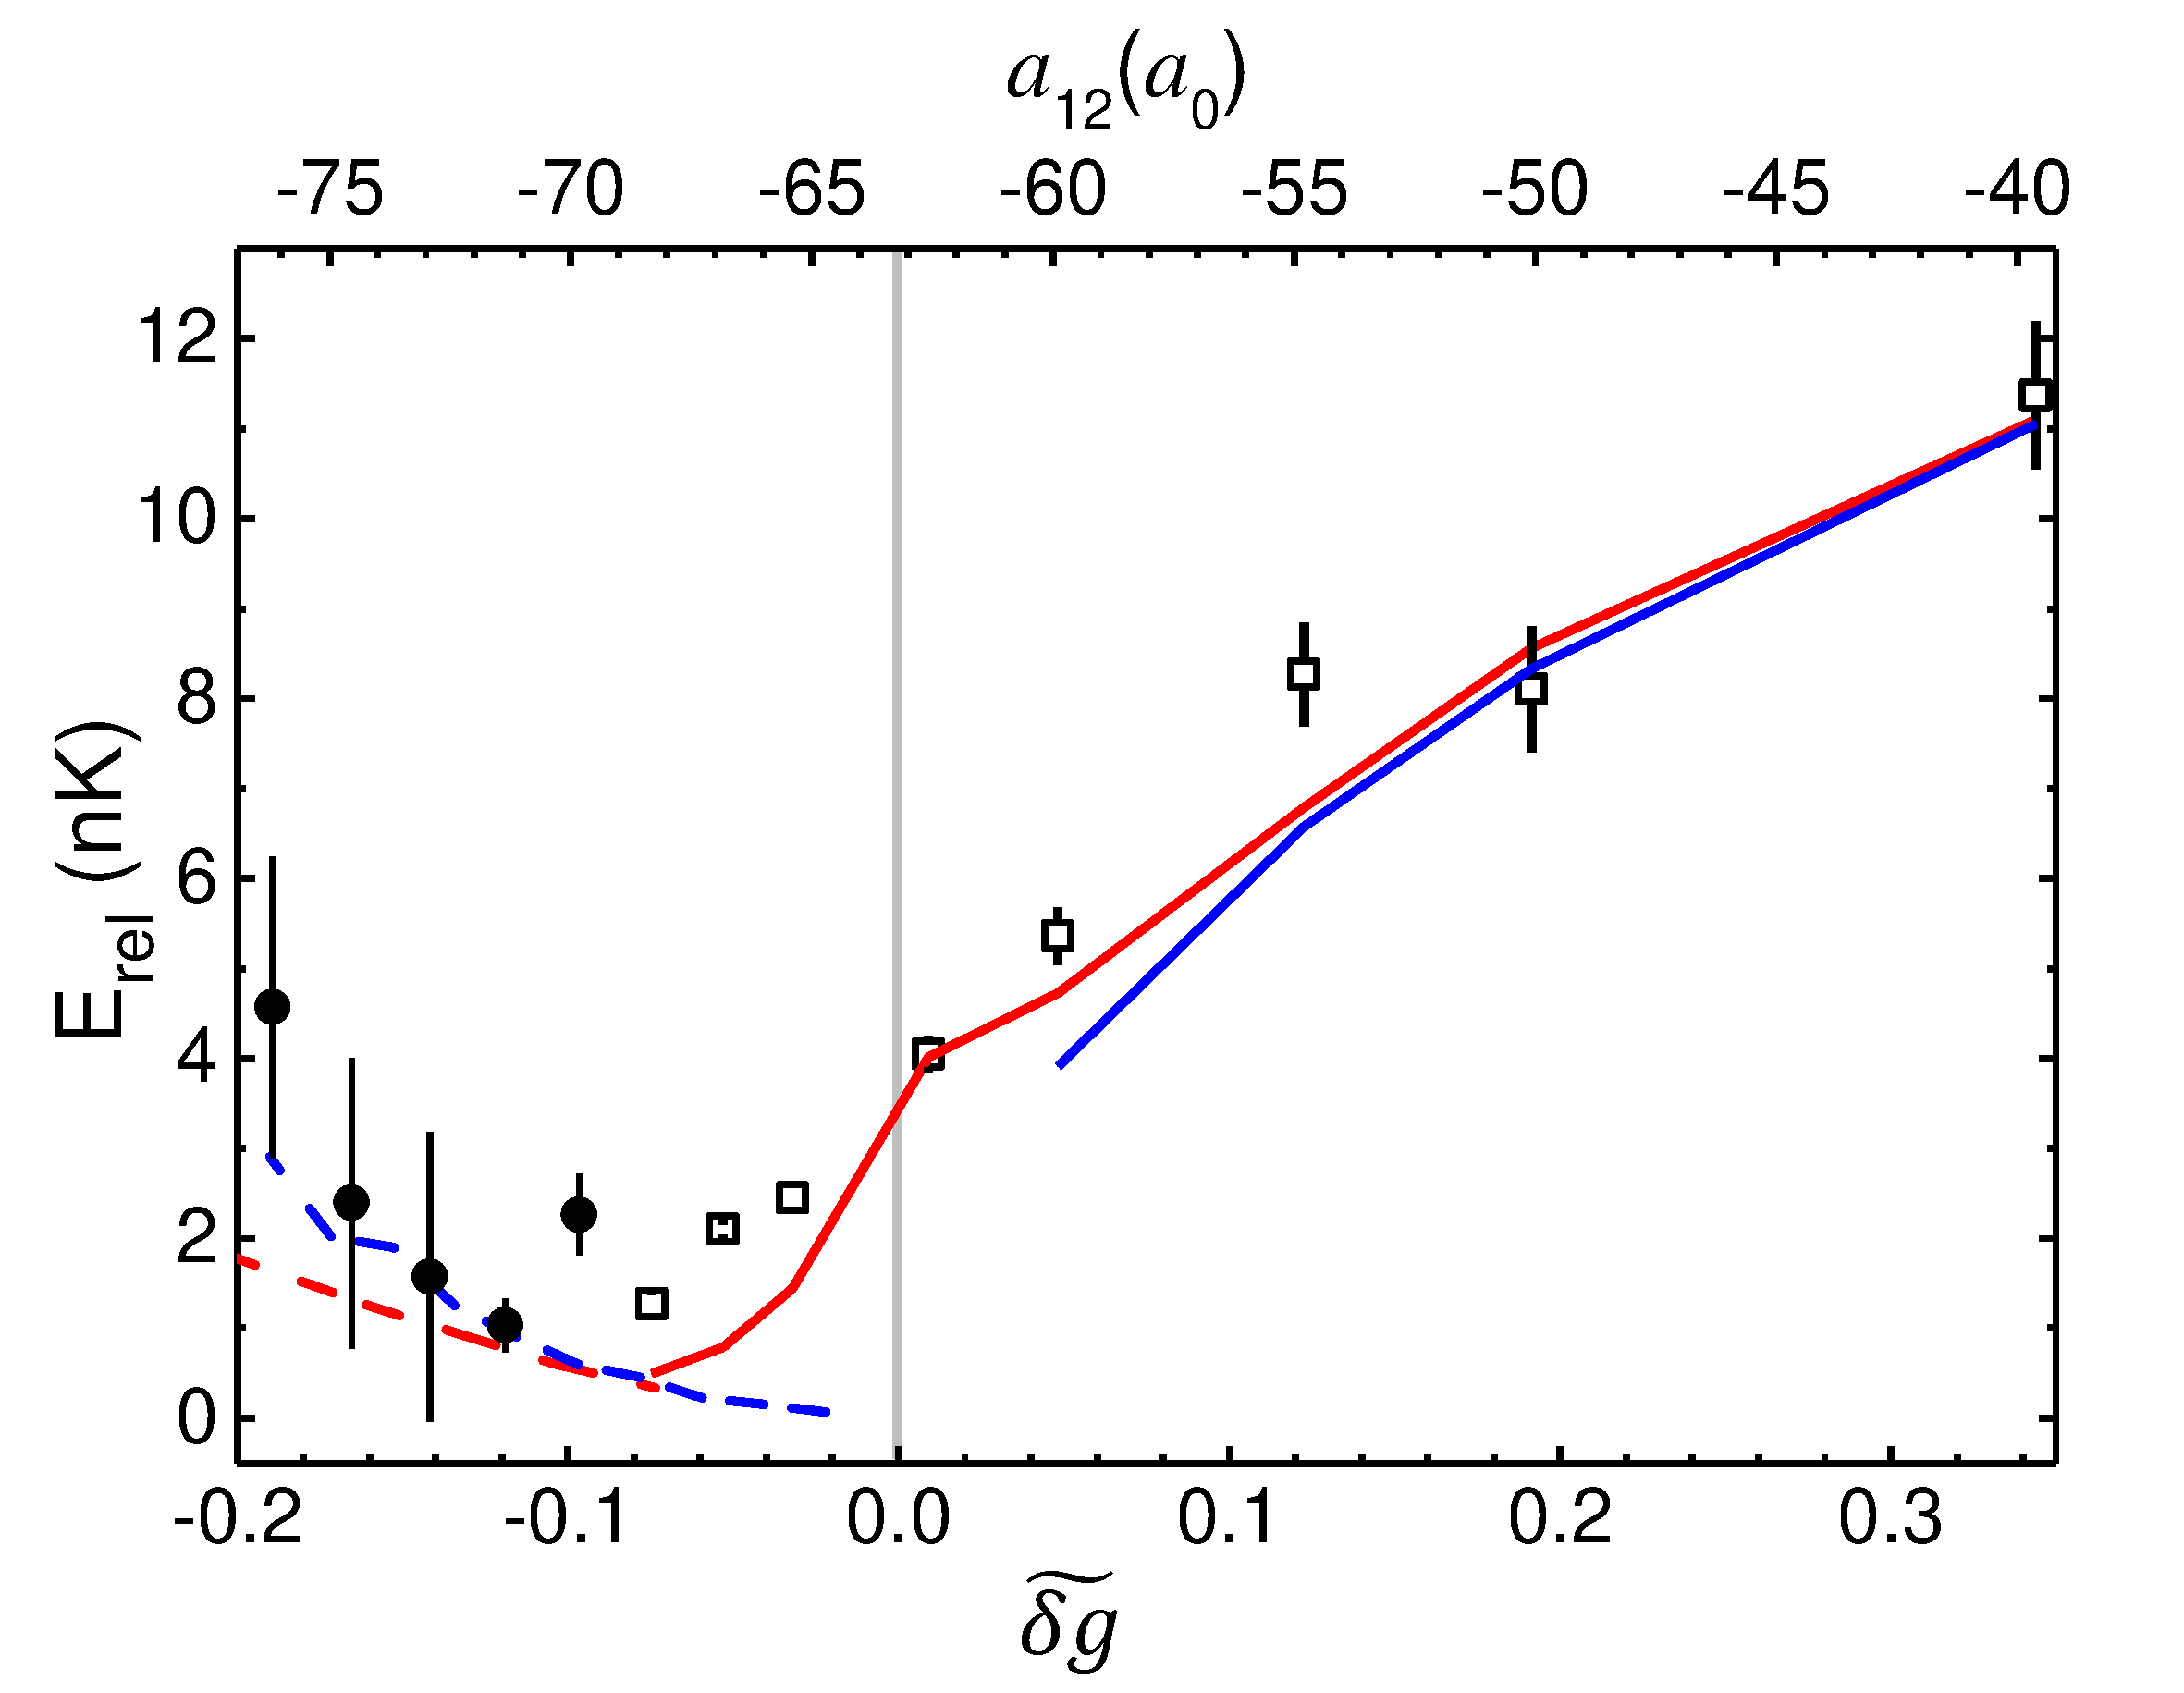
\includegraphics [width =0.85 \linewidth]{fig4.pdf}
\end{center}
\caption[Measurement of the release energy as a function of $\widetilde{\delta g}$]{Measurement of the release energy as a function of $\widetilde{\delta g}$. The open squares represent $E_{\rm rel}$ of the gas phase mixtures released from the trap directly, while the solid circles are $E_{\rm rel}$ of the gas samples formed following the liquid-gas phase transition. The red solid (blue solid) curve is the calculated $E_{\rm rel}$ with (without) the LHY terms for the first case with GPEs and the red dashed curve is $E_{\rm rel}$ for the second case from variational theory.}  
\label{fig4}
\end{figure}

We calculated the $E_{\rm rel}$ with the eGPEs for the corresponding atom numbers at the end of the TOF and found a good match for both the $E_{\rm MF}\gg E_{\rm LHY}$ and the $E_{\rm MF} \approx 0$ regions (red solid curve in Fig.~\ref{fig4}). We note that without the LHY term, the calculation fails for $\widetilde{\delta g} < 0$ due to the collapse (blue solid curve in Fig.~\ref{fig4}). At the $\widetilde{\delta g} \approx 0$ point with $E_{\rm MF}$ almost canceled, the energy difference between the two calculations is about $1$~nK. This is essentially the magnitude of $E_\text{\rm LHY}$, if we assume $E_{\rm kin}$ does not change dramatically in these two cases.   

The gas phase mixture formed following the liquid-to-gas phase transition is also of great interest. As shown in Fig.~\ref{fig2}(a), its expansion velocity can be measured and converted into another $E_{\rm rel}$ even though there is no trap involved. These results are shown in Fig.~\ref{fig4} as solid circles for $\widetilde{\delta g}$ from -0.146 to -0.247. Compared with the gas phase mixture released from the trap, the $E_{\rm rel}$ here has a completely opposite dependence on $\widetilde{\delta g}$. 

This behavior can be qualitatively understood from the change of the total energy of the droplet ($E_\text{tot}$) during the phase transition. For large enough atom numbers, $E_{\rm tot}$ has a negative minimum, and the system is in the droplet phase. Following the number loss, $E_{\rm tot}$ increases gradually. The droplet becomes meta-stable when $E_{\rm tot}$ is above zero, and the system eventually enters the gas phase when the energy minimum disappears. The measured $E_{\rm rel}$ here reflects $E_\text{tot}$ at the phase transition point which also includes contributions from $E_{\rm LHY}$, $E_{\rm MF}$, and $E_{\rm kin}$.

For more negative $\widetilde{\delta g}$, the critical atom numbers at the phase transition point are smaller, but the sample size $\propto |\widetilde{\delta g}|^{-3/2}$ shrinks much steeper. As result, the increase of the positive $E_{\rm LHY}$ and $E_{\rm kin}$ terms are faster than the decrease of the negative $E_{\rm MF}$ term. $E_{\rm tot}$ is thus positive and the measured $E_{\rm rel}$ also follows the same trend and increases for more negative $\widetilde{\delta g}$. We note that without $E_{\rm LHY}$, the magnitude of $E_{\rm MF}$ is larger than $E_{\rm kin}$ and the system will collapse. This picture is confirmed by the variational calculation as depicted by the red dashed curve in Fig.~\ref{fig4}.   

\section{Mode matching when producing droplet sample}
\label{sec:mode_match}

\subsection{In-trap vs. free-space sample}

During the release of the double BEC sample from the optical trap, the trap energy suddenly is removed suddenly but the size of the sample has no time to adapt to the new value. As shown in Fig.~\ref{figS1}, in general the in-trap size is smaller than the size of the ground-state free-space droplet at the energy minimum. The sample size will thus start to expand after released from the trap and its total energy (per particle) $E_{\rm tot} = E_{\rm kin} + E_{\rm int}$ will also start to evolve following the red curves. For the cases with very small $|\widetilde{\delta g}|$ [Fig.~\ref{figS1}(a)], $E_{\rm tot}$ is higher than the energy barrier at the right hand side. In this case, the sample will just keep expanding after crossing the maximum point and never forms the droplet. While in Fig. \ref{figS1}(b), with $|\widetilde{\delta g}|$ large enough, the negative $E_{\rm tot}$ of the released sample is not enough to overcome the energy barrier and the droplet can be formed, but its size will undergo a small-amplitude oscillation.

%% add figure-S1
\begin{figure}[hbt]
\begin{center}
\includegraphics [width = \linewidth]{figS1.pdf}
\end{center}
\caption[Droplet formation by directly releasing the trapped sample.]{Droplet formation by directly releasing the trapped sample. The blue dashed curves represent $E_{\rm tot} = E_{\rm kin}+E_{\rm pot}+E_{\rm int}$ of the trapped double BEC, and the red solid curves are $E_{\rm tot}$ in free space (i.e., $E_{\rm kin}+E_{\rm int}$). (a) For very small $|\widetilde{\delta g}|$, the free-space $E_{\rm tot}$ (the red open circle) is higher than the barrier height on the large size side (the red solid dot). In this case, the sample will keep expanding and never forms the droplet. (b) For $|\widetilde{\delta g}|$ large enough, the sample does not have enough energy and will be confined near the energy minimum to form the droplet.}
\label{figS1}
\end{figure}

\subsection{producing weak bound droplet by quenching B-field}

To improve the mode matching, we used a nearly spherical shape trap for matching the sphere shape of the quantum droplet. In addition, as the in-trap size of the double BEC also depends strongly on $\widetilde{\delta g}$, the magnetic field is controlled in a carefully designed sequence. After the double BEC is created, the magnetic field is first ramped up quickly across the Feshbach resonance to $358.4$~G where $a_{12}$ has a small positive value of $46.1a_0$. After 350 ms for the system to stabilize, the magnetic field is ramped down to 350.451 G in 130 ms. This is just 0.424 G above $B_c$ and the corresponding $a_{12}$ is $-39.5a_0$ ($\widetilde{\delta g} = +0.322$). Here the double BEC is miscible and the attractive interaction increases the spatial overlap of the two condensates and also increases the in-trap densities substantially. Both effects significantly improve the mode matching and facilitate the free-space droplet formation. At this point, rapid atom losses are already observed; thus, the magnetic field holds here for only 10 ms. Afterwards, the magnetic field is ramped to a target value within 5 ms before the droplet is detected in free space. As depicted in Fig.~\ref{figS1}(b), although droplet can be observed after these improvements for $|\widetilde{\delta g}|$ large enough, the mode matching is not perfect. For $\widetilde{\delta g}$ from 0 to -0.146, with the current atom numbers, the droplet cannot be observed by simply releasing the double BEC from the trap. As shown in Fig.~\ref{figS2}(a), even better mode matching can be achieved by finding a $\widetilde{\delta g}$ value where the in-trap size matches with the target droplet size and quenches $\widetilde{\delta g}$ at the same time when the trap is shut off. To achieve the fast magnetic field quenching necessary for this method, we added a small magnetic coil which is capable of covering the magnetic field range in less than 10 $\mu$s. Fig.~\ref{figS2}(b) and (c) show two droplets formed with this method. For case (b) with $\widetilde{\delta g} = -0.141$, the droplet lifetime is longer than the available observation time. For case (c) with $\widetilde{\delta g} = -0.110$, the liquid-to-gas phase transition is observed after about 7 ms. This short lifetime is probably limited by the atom numbers since at this $\widetilde{\delta g}$, the critical atom numbers are much larger.

\begin{figure}[hbtp]
\begin{center}
\includegraphics [width = 0.85 \linewidth]{figS2.pdf}
\end{center}
\caption[Producing long-lived droplet by magnetic field quench]{Producing long-lived droplet by magnetic field quench. (a) For some weakly bound droplet, it is possible to find a $\widetilde{\delta g}$ 
value where the in-trap gas-phase sample size (blue dashed curve) is the same as the size of the free-space droplet (red solid curve). Quenching $\widetilde{\delta g}$ at the instant of releasing the sample, as depicted by the black dashed arrow, will lead to a near perfect mode matching. (b) and (c) show the experimentally measured droplet signals for $\widetilde{\delta g} = -0.141$ (349.880 G) and $\widetilde{\delta g} = -0.110$ (349.910 G) created with this method. At these magnetic fields, no 
droplet can be observed without the quench as they fall in the situation as described in Fig.~\ref{figS1}(a).}
\label{figS2}
\end{figure}

%\section{producing Feshbach molecule from droplet}
%\label{sec:droplet_molecule}
%\chapter{Towards low dimension droplet}
\label{chap_LowD}

\section{Two-dimensional quantum droplet}
\subsection{2D scattering and interaction}
\subsection{quasi-2D and quasi-2D condition}
\subsection{quasi-2D droplet}
\subsection{Experiment Method and apparatus}
\subsection{}


\section{One-dimensional quantum droplet}
\chapter{Conclusion and Outlooks}
\label{chap:conclusion}

% epigraph
\setlength{\unitlength}{1pt}
\setlength{\epigraphwidth}{10cm}
\epigraph{What is a stupid question? If there is only one answer to the question instead of other possibility, it is a stupid question.}{--- Steven N. S. Cheung\\ \textit{Way of thinking (1984)}}

\section{Conclusion}
\section{Outlooks}

\chapterend



%=======================================================


%=======================================================
% Appendix and bibliography
\appendix
\includepdf[landscape=true,addtotoc={1,section,1,title in toc,cc},pages=1,offset=0cm 0.5cm]{FastCoilDriver_SCH.pdf}
\includepdf[addtotoc={1,section,1,title in toc,cc},pages=1-4,offset=0cm 0.5cm]{FastCoilDriver-SimuTinati.pdf}

% add mechanical design for image system up-down

% add 15x image system design 

% add ECDL 2D schematic
%\chapter{Extened Gross-Pitaevski equation simulation: GPELAB}
\label{chap:eGPELAB}

%\input{sections/S3_MOLSCAT}
\chapter{Camera comparison and absorption image SNR analysis}

\section{Absorption SNR analysis}

When doing absorption image, we typically take three images, noted as:
\begin{itemize}[noitemsep,topsep=0pt]
    \item \(C_{\text{in}}(x,y)\) as input light distribution on the atom
    \item \(C_{\text{out}}(x,y)\) as output(after absorption) light
    \item \(C_{\text{bg}}(x,y)\) as the background
\end{itemize}
formula of OD is
\begin{equation}
\text{OD}(x,y)=n_{\text{col}}(x,y)\sigma _0^*=\text{Log}\left[\frac{C_{\text{in}}(x,y)-C_{\text{bg}}(x,y)}{C_{\text{out}}(x,y)-C_{\text{bg}}(x,y)}\right]+\frac{C_{\text{in}}(x,y)-C_{\text{out}}(x,y)}{C_{\text{sat}}^{\text{eff}}}
\end{equation}
where
\begin{itemize}[noitemsep,topsep=0pt]
    \item \(C(x,y)=I(x,y)\times \frac{A_{\text{pix}}}{M^2}\times \frac{\lambda }{h c}\times T\times \text{QE}\times \tau \times \frac{1}{\text{ADC}}\)
    \item \(I(x,y)\) is the intensity distribution of light on atom
    \item \(A_{\text{pix}}\) is the pixel size of camera, \(\frac{A_{\text{pix}}}{M^2}\) is the real pixel size with counting magnification of image system.
    \item $\lambda $ is the probe light wavelength
    \item T is the transmission rate of the image system
    \item QE is the quantum efficiency of the camera
    \item ADC is the ADC conversion efficiency of the camera
    \item $\tau $ is the exposure time
\end{itemize}

The Noise is
\begin{equation}
\begin{split}
\sigma _{\text{OD}}^2&=\left(\frac{\partial \text{OD}}{\partial C_{\text{in}}}\right){}^2\sigma _{C_{\text{in}}}^2+\left(\frac{\partial \text{OD}}{\partial C_{\text{out}}}\right){}^2\sigma _{C_{\text{out}}}^2+\left(\frac{\partial \text{OD}}{\partial C_{\text{bg}}}\right){}^2\sigma _{C_{\text{bg}}}^2\\
&=\left(\frac{1}{C_{\text{sat}}^{\text{eff}}}+\frac{1}{C_{\text{in}}-C_{\text{bg}}}\right){}^2\sigma _{C_{\text{in}}}^2+\left(\frac{1}{C_{\text{sat}}^{\text{eff}}}+\frac{1}{C_{\text{out}}-C_{\text{bg}}}\right){}^2\sigma_{C_{\text{out}}}^2\\
&+\left(\frac{1}{C_{\text{in}}-C_{\text{bg}}}-\frac{1}{C_{\text{out}}-C_{\text{bg}}}\right){}^2\sigma _{C_{\text{bg}}}^2
\end{split}
\end{equation}

Then, The Signal to Noise ratio is
\begin{equation}
\begin{split}
\text{SNR}&=\frac{\text{Log}\left[\frac{C_{\text{in}}-C_{\text{bg}}}{C_{\text{out}}-C_{\text{bg}}}\right]+\frac{C_{\text{in}}-C_{\text{out}}}{C_{\text{sat}}^{\text{eff}}}}{\sqrt{\alpha^2+\beta^2+\gamma^2}}\\
\alpha^2&=\left(\frac{1}{C_{\text{sat}}^{\text{eff}}}+\frac{1}{C_{\text{in}}-C_{\text{bg}}}\right){}^2\sigma_{C_{\text{in}}}^2\\
\beta^2&=\left(\frac{1}{C_{\text{sat}}^{\text{eff}}}+\frac{1}{C_{\text{out}}-C_{\text{bg}}}\right){}^2\sigma _{C_{\text{out}}}^2\\
\gamma^2&=\left(\frac{1}{C_{\text{in}}-C_{\text{bg}}}-\frac{1}{C_{\text{out}}-C_{\text{bg}}}\right){}^2\sigma
_{C_{\text{bg}}}^2
\end{split}
\end{equation}

Put noise formula into the above SNR, we have

\begin{equation}
\begin{split}
\text{SNR}&=\frac{\text{Log}\left[\frac{C_{\text{in}}-C_{\text{bg}}}{C_{\text{out}}-C_{\text{bg}}}\right]+\frac{C_{\text{in}}-C_{\text{out}}}{C_{\text{sat}}^{\text{eff}}}}{\sqrt{X^2+Y^2+Z^2+W^2}}\\
X^2&=\left[\left(\frac{1}{C_{\text{sat}}^{\text{eff}}}+\frac{1}{C_{\text{in}}-C_{\text{bg}}}\right){}^2+\left(\frac{1}{C_{\text{sat}}^{\text{eff}}}+\frac{1}{C_{\text{out}}-C_{\text{bg}}}\right){}^2\right.\\
&\left.+\left(\frac{1}{C_{\text{in}}-C_{\text{bg}}}-\frac{1}{C_{\text{out}}-C_{\text{bg}}}\right){}^2\right]\sigma_{\text{readout}}^2\\
Y^2&=\left(\frac{1}{C_{\text{sat}}^{\text{eff}}}+\frac{1}{C_{\text{in}}-C_{\text{bg}}}\right){}^2\sigma _{\text{in}-\text{signal}}^2\\
Z^2&=\left(\frac{1}{C_{\text{sat}}^{\text{eff}}}+\frac{1}{C_{\text{out}}-C_{\text{bg}}}\right){}^2\sigma_{\text{out}-\text{signal}}^2\\
W^2&=\left(\frac{1}{C_{\text{in}}-C_{\text{bg}}}-\frac{1}{C_{\text{out}}-C_{\text{bg}}}\right){}^2\sigma _{\text{bg}-\text{signal}}^2
\end{split}
\end{equation}

\begin{table}[hbt]
\caption[Cameras parameter table]{Camera parameter table}
\label{camera_test}
\begin{tabular}{|l|l|l|l|l|}
\hline
                                                                               & PCO-Pixelfly & GS3-U3-15S5M-C & BFS-PGE-31S4 & PCO-sCOS \\ \hline
Wavelength(nm)                                                                 & 589/780      & 589/780        & 589/780      & 589/780  \\ \hline
QE(\%) on datasheet                                                            & 58/25        & 72/35          & 70/30        & 61/35    \\ \hline
QE(\%) measured                                                                & -/22.0       & 56.6/-         & 47.2/27.0    &          \\ \hline
\begin{tabular}[c]{@{}l@{}}Readout noise(e)\\ on datasheet\end{tabular}        & 6            & 8.31           & 2.29         & 1.1      \\ \hline
\begin{tabular}[c]{@{}l@{}}Readout noise(e)\\ measured\end{tabular}            &              &                & 0.53         &          \\ \hline
\begin{tabular}[c]{@{}l@{}}Dark noise rate\\ on datasheet\end{tabular}         & 1 e/s        &                &              & 0.8 e/s  \\ \hline
\begin{tabular}[c]{@{}l@{}}Dark noise rate\\ measured\end{tabular}             &              &                & 0.59 e/s     &          \\ \hline
\begin{tabular}[c]{@{}l@{}}A/D conversion(e/count)\\ on datasheet\end{tabular} & 1            & tunable        & tunable      & 0.46     \\ \hline
\begin{tabular}[c]{@{}l@{}}A/D conversion(e/count)\\ measured\end{tabular}     &              &                & 1/0.53       &          \\ \hline
\end{tabular}
\end{table}
\newpage
\setstretch{1}
\bibliography{database}
%=======================================================
\end{document}